
% Chargement de la classe Framaquette
\documentclass{framatexclass}

% Thermodynamique
\usepackage{framabook_thermo} 			% styles spéciaux thermo
\usepackage{framabook_metathermo} 		% contenus spéciaux thermo

%\usepackage{showframe}			% pour débugger la maquette
%\includeonly{10/chapitre_10}	% pour n’inclure qu’un chapitre

\begin{document}

\frontmatter
% Blabla disclaimer temporaire
	\widecenteredpagegeometry
	\thispagestyle{empty}
		\vspace*{\stretch{1}}
			\begin{center}
				{\Large\textit{Work in Progress}}

				Ce document est un prototype. Un wiki de travail est en ligne à l’adresse\\
				\href{http://dokuwiki.framabook.org/doku.php?id=framabookthermodynamique}{dokuwiki.framabook.org/doku.php?id=framabookthermodynamique} ;
				
				Le code source du livre et ses mises à jour sont consultables à l’adresse 
				\href{https://github.com/ariadacapo/thermodynamique}{github.com/ariadacapo/thermodynamique}

				Mise à jour de ce document : \today
			\end{center}
		\vspace*{\stretch{1}}
	\restoregeometry
	

% Page de titre intérieure
	\newgeometry{left=1cm,right=1cm,top=1cm,bottom=1cm}
\begin{titlepage}
\vspace*{4cm}
\begin{center}
	\vspace{1em}\par \rule{15cm}{.1pt}
	{\HUGE Thermodynamique\\ de l’ingénieur}
	\vspace{1em}\par \rule{15cm}{.1pt}

	\vspace{4cm}
	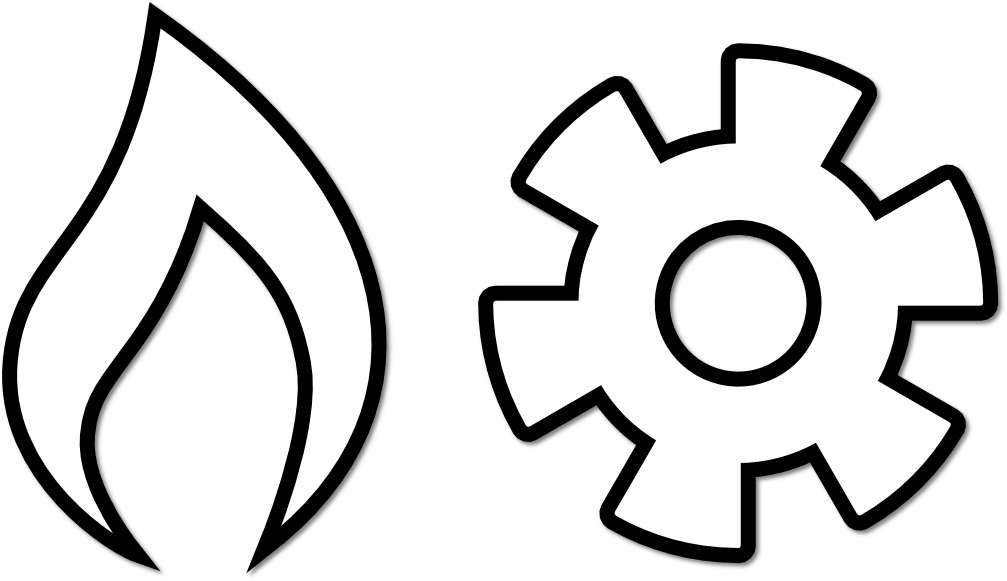
\includegraphics[width=8cm]{images/thermodynamics.png}
	\vspace{2cm}

	{\huge Olivier Cleynen}
	
	\hspace{0.5cm}
\includegraphics[width=60mm]{images/Logo_framabook_grand.png}
\end{center}

\clearpage


\restoregeometry\pagestyle{empty}
\vspace*{5cm}
	Framasoft est un réseau d’éducation populaire, issu du monde éducatif, consacré principalement au logiciel libre. Il s’organise en trois axes sur un mode collaboratif : promotion, diffusion et développement de logiciels libres, enrichissement de la culture libre et offre de services libres en ligne.\\
	Pour plus d’informations sur Framasoft, consultez \href{http://framasoft.org/}{http://framasoft.org/}.
	
	Se démarquant de l’édition classique, les Framabooks sont dits «~livres libres~» parce qu’ils sont placés sous une licence qui permet au lecteur de disposer des mêmes libertés qu’un utilisateur de logiciels libres. Les Framabooks s’inscrivent dans cette culture des biens communs qui favorise la création, le partage, la diffusion et l’appropriation collective de la connaissance.\\
	Pour plus d’informations sur le projet Framabook, consultez \href{http://framabook.org/}{http://framabook.org/}.

\vspace*{\stretch{4}}
\begin{center}
		\noindent Copyright 2015 Olivier Cleynen, Framasoft (collection Framabook)\\
		\textit{Thermodynamique de l’ingénieur} est placé sous licence Creative Commons :\\
		\ccLogo\ \ccAttribution\ \ccShareAlike \ \ \href{https://creativecommons.org/licenses/by-sa/4.0/deed.fr}{Attribution -- Partage dans les Mêmes Conditions 4.0}.\\
		Les termes de la licence sont détaillés en annexe~\ref{ch_remix} p.\pageref{ch_remix}.
		
		{\footnotesize Couverture : schéma \ccbysa par Olivier Cleynen, dérivé d’\wcfile{HOP ATR42 F-GPYC 25sep14 LFBO-2.jpg}{une photo} \ccbysa par \wcu{Gyrostat}. Pingouin du logo Framasoft \lal \href{http://www.le-terrier.net/pingouin/pingouin.html}{par LL de Mars}.\par}

		\noindent Dépôt légal : Avril 2015\\
		Prix : 19 euros\\
		ISBN : 979-10-92674-08-8
\end{center}


\end{titlepage}
\pagestyle{fancy}\restoregeometry

	
% Auteurs
	\clearpage
\pagestyle{empty}

\chapter*{Auteurs} % comme tout le monde s’en fout, on ne les met pas dans la TOC
\thispagestyle{empty}

	../../contenu/Annexes/contenu_auteurs.tex

\pagestyle{fancy}

		%ce fichier appelle contenu_auteurs.tex

% Table des matières
	\clearpage
\widecenteredpagegeometry
\pagestyle{empty}

	\tableofcontents{}\thispagestyle{empty}

\restoredefaultfootersandheaders
\restoregeometry


% Organisation de l’ouvrage
	Ce livre a pour objectif de vous permettre de comprendre, décrire et quantifier le fonctionnement des machines thermodynamiques, c’est-à-dire les réfrigérateurs, les pompes à chaleur, et surtout les moteurs. Il est conçu pour être abordable en première année d’études supérieures et couvert en deux semestres environ. Il est destiné à de futur/es ingénieur/es curieux/ses de comprendre le pourquoi et le comment des machines qui les entourent et des équations qu’ils ou elles utilisent.

Il y a dix chapitres dans ce livre. Le \coursun recense les notions indispensables à notre étude, comme l’énergie, le travail, la chaleur et la température.

Le chapitre le plus important est le \courssix~: c’est là que nous apprenons à transformer de la chaleur en travail et réciproquement. Cependant, pour pouvoir appliquer les concepts de ce chapitre à des cas concrets —~par exemple pour pouvoir prédire par le calcul l’efficacité d’un moteur~— nous avons besoin de plusieurs outils, auxquels sont consacrés les chapitres qui précèdent. Il nous faut d’abord disposer d’une méthode robuste de comptabilité de l’énergie : dans le \coursdeux nous comptabilisons les transferts dans une quantité fixe de fluide, et dans le \courstrois nous comptabilisons ces transferts dans un fluide en flux continu. Il nous faut également savoir prédire la température et quantifier l’énergie dans les fluides utilisés en pratique, ce que nous faisons pour l’air dans le \coursquatre et pour l’eau dans le \courscinq. Ainsi, à la fin du \courssixshort, vous saurez quantifier la transformation de chaleur et de travail au sein de tous types de machines.

Une particularité des machines thermodynamiques est qu’elles sont toutes très inefficaces. L’exploration des causes de ces inefficacités et la quantification de leurs limites théoriques font l’objet du \courssept. Cette exploration culmine avec le \courshuitshort où nous apprenons à nous servir de l’\textit{entropie}, un extraordinaire et puissant concept physique, pour décrire les transformations dans nos machines.

Avec ces notions, vous serez à même de comprendre et quantifier le fonctionnement de deux grands types de moteurs utilisés dans l’industrie : les centrales à vapeur, décrites dans le \coursneuf, et les moteurs à combustion interne, décrits dans le \coursdix.

\onlyamphibook{\clearpage\thispagestyle{empty}}%handmade
\begin{center}
	\onlyframabook{\vspace{1cm}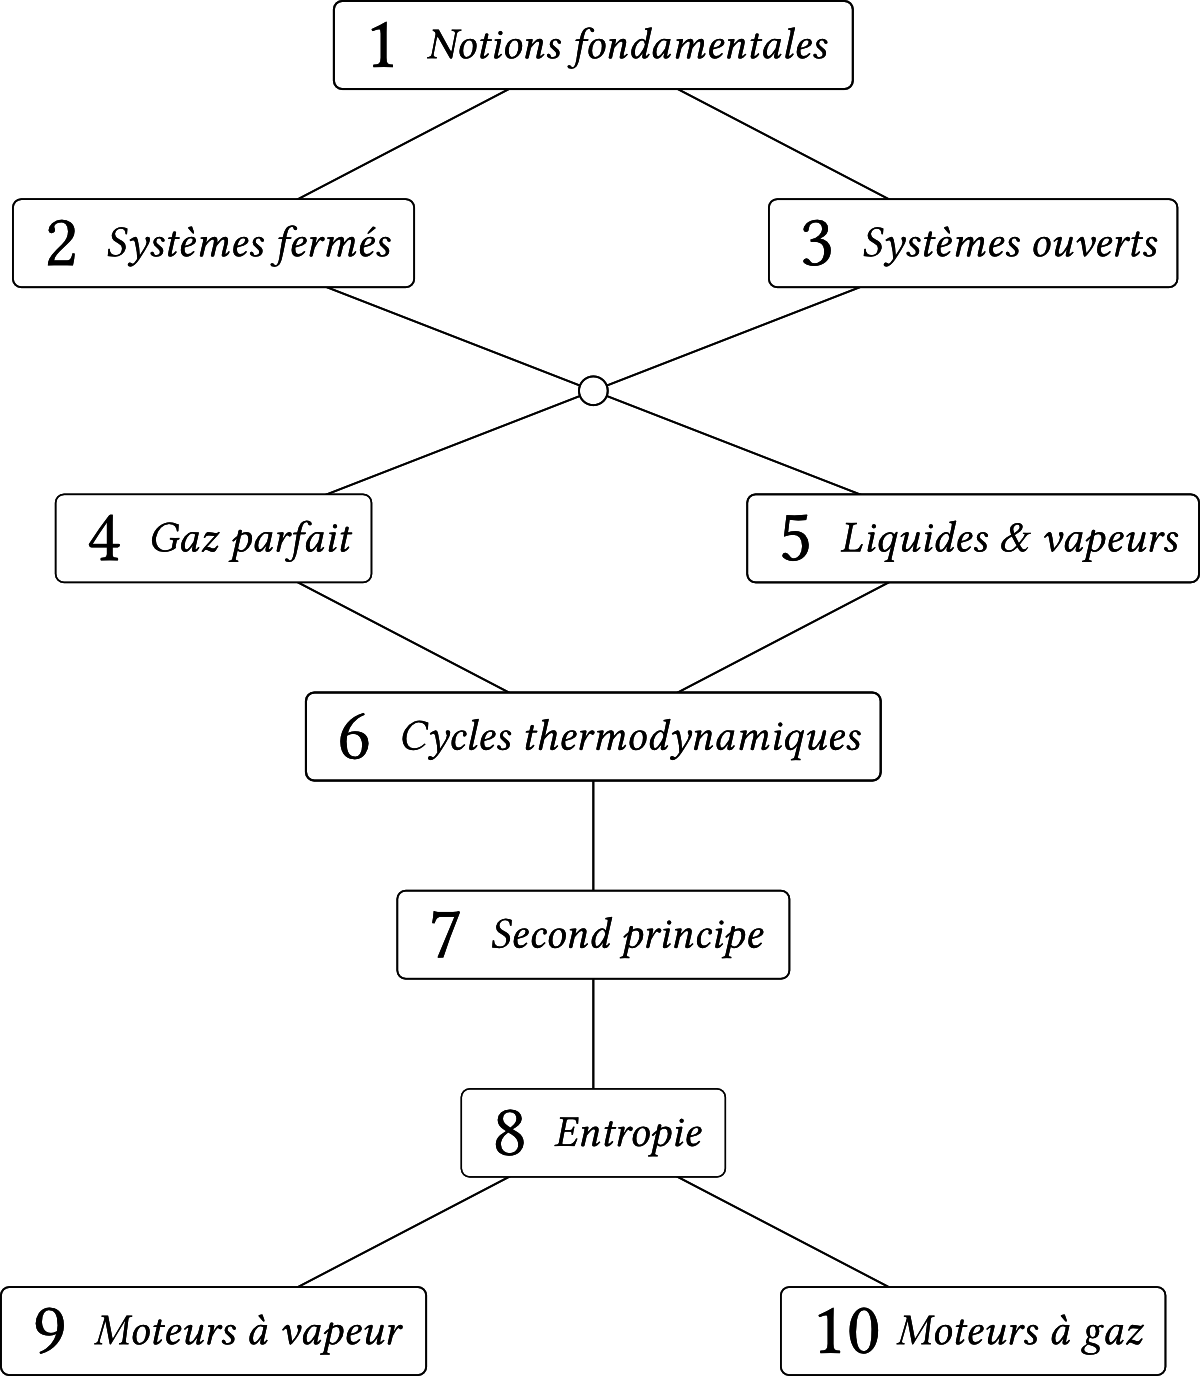
\includegraphics[width=0.7\textwidth]{images/plan_general_chapitres.png}\vspace{1cm}}%handmade
	\onlyamphibook{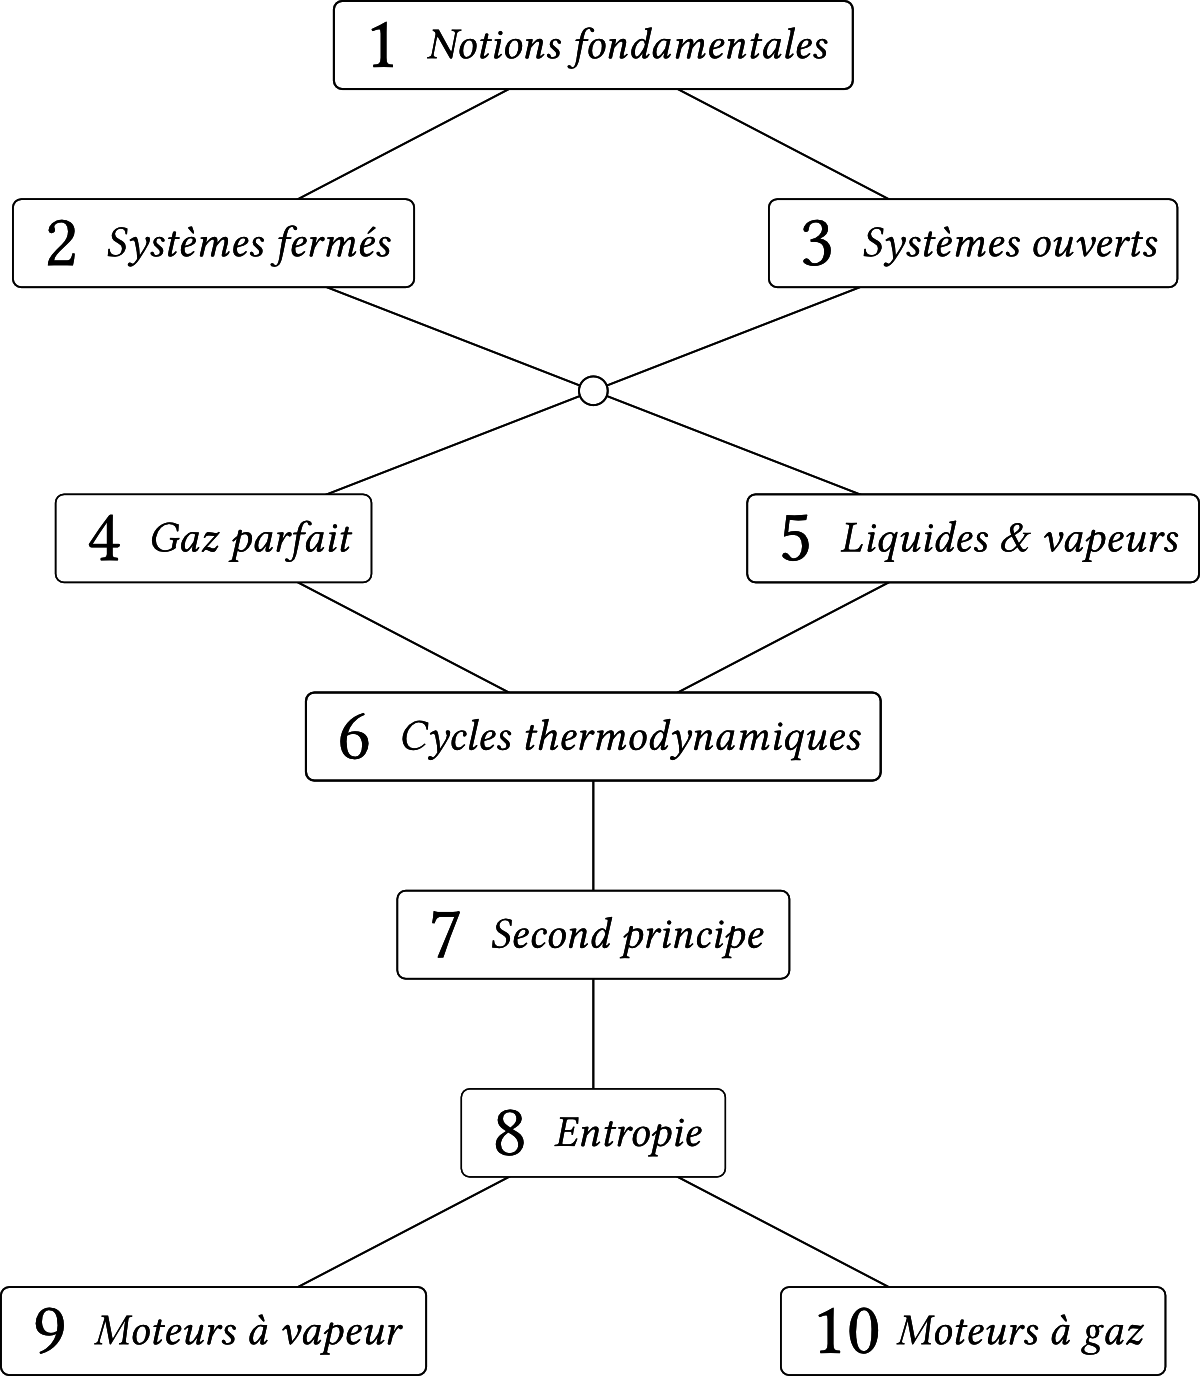
\includegraphics[width=0.65\textwidth]{images/plan_general_chapitres.png}}
\end{center}

À la fin de chaque chapitre, une série de problèmes concrets est présentée. Ces exercices sont là pour votre entraînement, mais aussi pour votre motivation : ils présentent le type de problème que nous cherchons à résoudre avec le chapitre. Afin de vous permettre de vous former seul/e, la solution de chaque exercice est brièvement décrite en dernière page. Je vous conseille de ne jamais y avoir recours avant d’avoir transpiré au moins une heure, car une fois que l’on a lu la méthode de résolution, il est impossible de faire comme si l’on ne la connaissait pas !

Vous trouverez aussi à la fin de chaque chapitre une courte section historique. Ces petits éléments de contexte nous ont semblé, à moi-même et Philippe Depondt, pouvoir contribuer à votre culture de scientifique et d’ingénieur/e. 

Enfin, le livre que vous avez entre les mains est véritablement \emph{à vous} : il est publié sous une licence libre dont les termes sont détaillés en annexe~\ref{ch_remix}. Il me paraît en effet important que vous puissiez non seulement le partager librement et gratuitement (en le photocopiant, en en faisant des copies numériques, etc.) mais aussi le remixant d’une façon ou d’une autre (en l’améliorant, le raccourcissant ou l’adaptant à d’autres formes par exemple) en fonction de vos besoins, vous appropriant ainsi véritablement son contenu.

Mon espoir est qu’après avoir utilisé ce livre, le son d’une turbomachine en fonctionnement ne puisse vous laisser ni perplexe ni insensible. Bon courage !

\begin{flushright}Olivier Cleynen\\ \textit{février 2015}\end{flushright}

	
% Intro
	\clearpage
\pagestyle{empty}

\chapter*{Introduction} % comme tout le monde s’en fout, on ne la met pas dans la TOC
\thispagestyle{empty}

	La thermodynamique est l’étude de la conversion de l’énergie entre deux formes, chaleur et travail. Pourtant, ses débuts remontent bien avant que ces trois concepts ne soient établis : pendant longtemps il ne s’est agi que de se pencher sur \emph{la nature de la chaleur}. Autrement dit, que veut dire «~chaud~» exactement ? Peut-on le mesurer ?

Les premières réflexions sur la nature de la matière, et celle du feu, datent de la Grèce antique, et donnent déjà naissance à la théorie atomique. Mais il ne s’agit alors que de constructions philosophiques, plus fondées sur une vision spirituelle organisée du monde que sur de réels travaux d’observation.

Il faudra attendre les années 1600 pour que débutent de sérieux travaux de recherche. C’est la température, dont on se fait plus facilement une idée que de la chaleur, qui est d’abord le centre  d’intérêt. La conception du thermomètre soulève en effet de nombreux problèmes d’ingénierie et de physique : comment lier cette idée de «~température~» à un phénomène observable directement, de façon prévisible et reproductible ?

Pendant ces années et jusqu’en 1850, la thermodynamique reste à l’échelle macroscopique –~il n’est pas encore question d’atome ou de molécule. Elle suscite beaucoup d’intérêt parce qu’elle aborde directement les phénomènes de frottement et de transfert de chaleur, qui ne se produisent jamais que dans un seul sens, et auxquels une vision mécanique newtonienne de l’univers ne peut fournir d’explication.

Le grand essor des machines thermiques, au début du \textsc{xix}\ieme siècle, prend la science de court. Les premiers moteurs pompent l’eau hors des mines, mais la thermodynamique –\ qui ne porte alors même pas son nom\ – ne sait pas expliquer comment. Il faudra une trentaine d’années avant que la théorie ne rattrape la pratique, et que l’on établisse une vision cohérente de la thermodynamique permettant, par exemple, de prévoir le rendement d’un moteur.

En 1865, Clausius clôture près d’un siècle de tâtonnements en explicitant les grandes bases de ce que l’on commence à appeler «~thermodynamique~» : c’est ce que nous connaissons aujourd’hui sous le nom des deux principes. Il généralise, ce faisant, ses observations sur un ballon de gaz à l’univers tout entier. 
De leur côté, Maxwell et Boltzmann réconcilieront la thermodynamique avec la physique telle que nous la connaissons aujourd’hui. Au fur et à mesure du \textsc{xx}\ieme siècle, le concept d’incertitude se fait accepter et la thermodynamique devient affaire de probabilités et de quantification du désordre ; elle sert même à poser les bases de la théorie de l’information.

Entre temps, la révolution industrielle a eu lieu. Délaissant la pompe à eau, le moteur thermique est passé à la propulsion des locomotives, puis navires, automobiles, génératrices de courant, et aéronefs. Notre mode de vie, dans lequel la force physiologique humaine n’a plus la moin\-dre importance, montre à quel point  nous som\-mes devenus dépendants de la puissance et de la précision qu’il permet. Le moteur à chaleur, en somme, est la raison pour laquelle notre environnement diffère tant de celui de nos ancêtres, et de celui que connaîtront nos descendants. La thermodynamique permet de comprendre le fonctionnement déroutant de cet engin à la fois banal et effroyable.

Au cours de cette série de dix chapitres sur la \textit{thermodynamique de l’ingénieur}, nous passerons du comportement élémentaire des fluides à la théorie des moteurs –\ l’objectif étant de fournir à l’étudiant/e une bonne compréhension du fonctionnement des machines à chaleur et une base solide pour pouvoir aborder la conception moteur et la mécanique des fluides.



\pagestyle{fancy}

		%ce fichier appelle contenu_introduction.tex


\mainmatter
\renewcommand{\nomducours}{\nomcoursun}
\renewcommand{\sousnomducours}{\sousnomcoursun}
\renewcommand{\chapterlabel}{chap_un}

\olivierschapterpage{\nomducours}{\sousnomducours}

\olivierscontentpage{\contentsummarycoursun}

\section*{Introduction}
Nous posons ici les concepts indispensables dont nous nous servirons dans les chapitres à venir, en tentant de répondre à deux questions :
\begin{itemize}
	\item Que représente l’énergie ?
	\item Quelles formes d’énergie manipule-t-on dans une machine ?
\end{itemize}
\dontbreakpage \vspace{2em}
\section{Démarche}

	L’objectif de cet ouvrage est de décrire les caractéristiques physiques des principaux moteurs de l’industrie. Pour pouvoir décrire leurs performances et leurs limites, il nous faut commencer un étage plus bas, en nous posant d’abord des questions comme :
	
		\begin{itemize}
			\item Comment et pourquoi un moteur peut-il fonctionner ? Comment transformer de la chaleur en travail ?
			\item Comment peut-on refroidir un objet ? Comment peut-on inverser le sens spontané des transferts de chaleur ?
		\end{itemize}

	Or, pour pouvoir donner des réponses solides à ces questions, il faut bien maîtriser les notions de chaleur, de température, et de travail ; ainsi nous devons d’abord descendre encore quelques étages plus bas :
	
		\begin{itemize}
			\item Comment quantifie-t-on la chaleur et le travail dans une machine ?
			\item Comment un fluide peut-il recevoir ou fournir de l’énergie ?
			\item Que représentent l’énergie, la chaleur, et la température ?
		\end{itemize}

	Ces questions sont le cœur de ce que nous appelons \vocab{thermodynamique}, c’est-à-dire l’étude de la nature de la chaleur. Nous allons devoir commencer tout en bas, et nous remonterons progressivement jusqu’à pouvoir enfin expliquer pourquoi l’efficacité d’un moteur Diesel dépasse rarement \SI{40}{\percent}. En route !
	
\section{Notion d’énergie}

	\subsection{L’énergie}
	\label{ch_energie}
	
		Nous nous attaquons d’emblée à l’une des notions les plus difficiles de toute la physique : l’\vocab{énergie}.
		
		Nous observons que dans tous les phénomènes, lors de toutes les transformations que nous pouvons observer dans l’univers, il existe une grandeur qui ne varie pas. Cette grandeur quantifie une propriété abstraite (énergie vient du grec \textgreek{ἐνέργεια}, \textit{energeia}, soit «~activité~», «~opération~») qui peut prendre de multiples formes. %On peut penser la notion d’énergie comme étant la capacité à mettre un objet en mouvement.
		
		Nous avons appris à compter la quantité d’énergie présente dans n’importe quel volume arbitraire, et nous nous attachons à contrôler sa transformation d’une forme à une autre. Par exemple, l’énergie électrique stockée dans une batterie peut être transformée en travail dans un moteur électrique, ce qui peut servir à actionner un ascenseur, qui peut soulever une charge. Lors de toutes ces évolutions, la quantité totale d’énergie reste la même (\cref{fig_crashed_car}), un fait qui nous permet par exemple de quantifier la taille minimale de batterie nécessaire pour soulever une charge donnée.
		
		\begin{figure}
			\begin{center}
				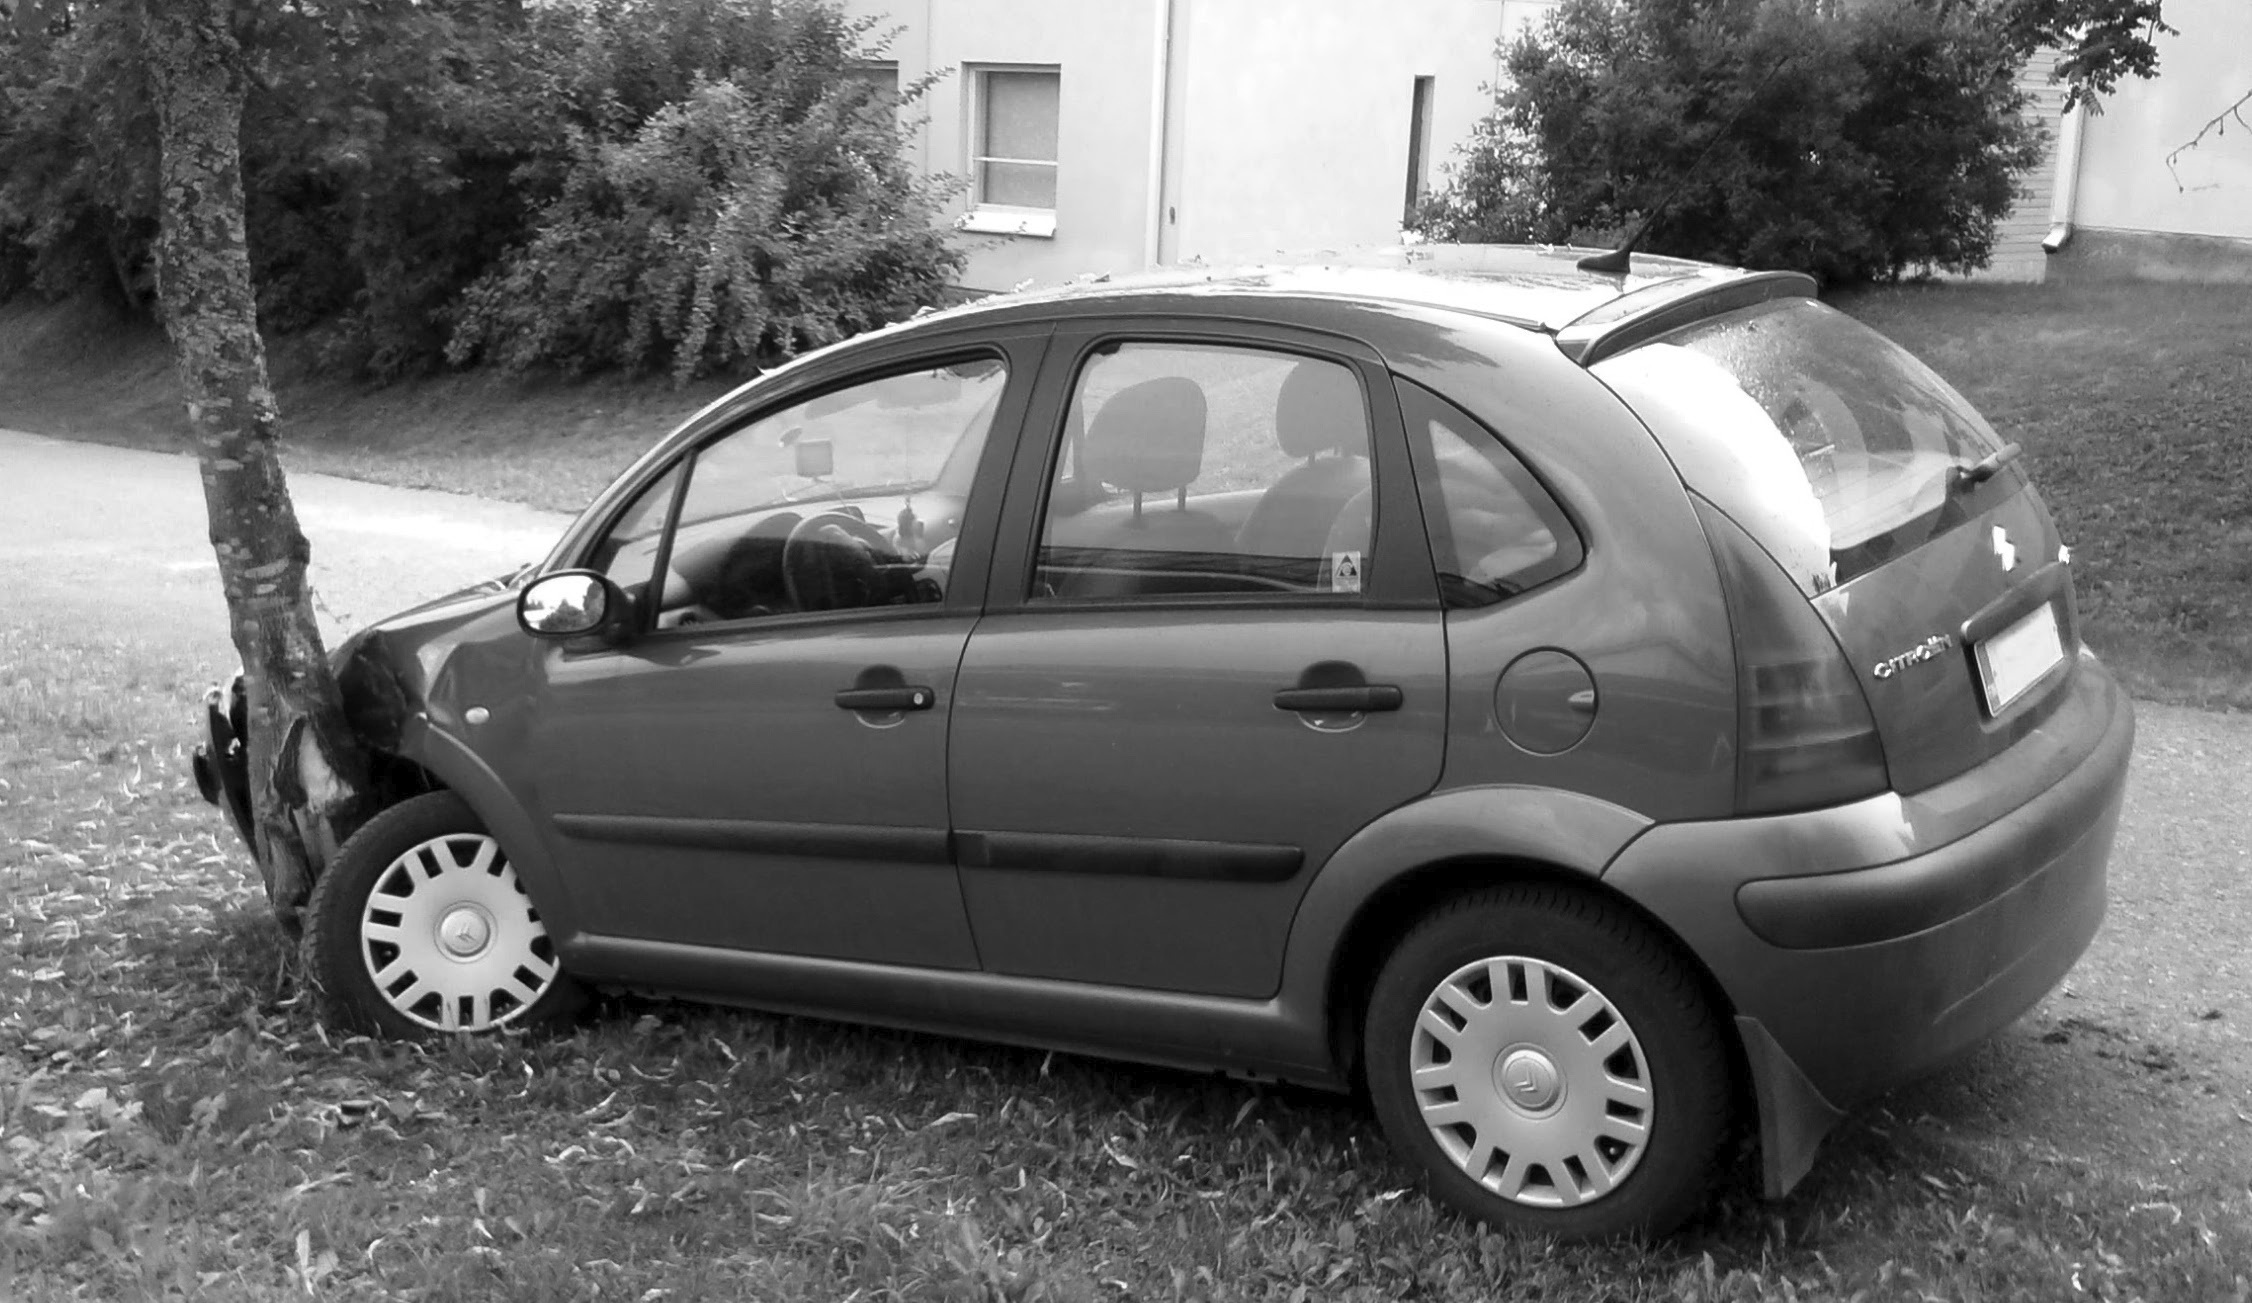
\includegraphics[width=0.5\textwidth]{images/crashed_citroen_c3.jpg}
			\end{center}
				\supercaption{L’énergie chimique stockée dans le carburant qui a été consommé est exactement égale à l’énergie rejetée par le pot d’échappement, plus l’énergie dissipée par frottement, plus l’énergie cinétique de la voiture en route. Toute cette énergie est transformée en chaleur, \emph{mais jamais détruite}, une fois la voiture arrêtée (quelqu’en soit le moyen !).}{Photo dérivée d’\wcfile{Crashed Citroën C3 (2).jpg}{une photo} \ccbysa par \wcun{Tommi_Nummelin}{Tommi Nummelin}}
			\label{fig_crashed_car}
		\end{figure}
		
		Ainsi, l’énergie est surtout un concept que nous utilisons pour lire les transformations que nous observons dans le monde : nous pourrions dire que c’est «~ce qui ne change pas lorsque les choses se transforment~». Pour l’ingénieur, elle représente surtout la capacité d’un corps à en mettre un autre en mouvement, de façon unifiée (par exemple avec un déplacement) ou désordonnée (par exemple avec une excitation chaotique).

		Nous mesurons l’énergie en \si{joules} (\si{\joule}).
	
	\subsection{Le premier principe}
		\label{ch_premier_principe}

		Le \vocab{premier principe de la thermodynamique} affirme simplement :

		\begin{principe}
				L’énergie est indestructible.
		\end{principe}

			\thermoquotebegin{O}
			Il est important de réaliser que dans la physique d’aujourd’hui, nous n’avons aucune connaissance de ce \emph{qu’est} l’énergie. Nous n’avons pas de représentation comme quoi l’énergie viendrait en petit paquets d’une certaine quantité. Cependant des formules permettent de calculer une quantité numérique, et lorsque nous les additionnons toutes, nous obtenons toujours le même nombre. C’est une chose abstraite en cela qu’elle ne nous donne pas le mécanisme ou les \emph{raisons} des différentes formules.
		\thermoquoteend{Richard Feynman, 1963}{\textit{The Feynman Lectures on \mbox{Physics}} \mbox{\cite{feynman1963, feynman1963fr}}}

		On peut aussi écrire que «~l’énergie de l’univers est constante~», ou «~l’énergie se conserve toujours~» : elle ne peut être ni créée ni détruite. Autrement dit, lorsqu’un objet reçoit un \si{joule} d’énergie, il peut soit l’emmagasiner, soit le re-fournir à l’extérieur ; mais en aucun cas il ne peut le détruire.

		Il n’y a que deux principes importants en thermodynamique ; le second (auquel nous consacrons les chapitres~\sept et~\huit) porte lui aussi sur la nature de l’énergie. Leurs implications sont énormes et ils sont le fruit d’un travail intellectuel profond et laborieux, long de plusieurs siècles. Il n’existe pas de preuve ou de démonstration de leur véracité, mais toutes nos observations et expériences les corroborent, de sorte qu’ils sont aujourd’hui universellement acceptés.
		
		Nous exprimerons quantitativement le premier principe de deux façons différentes, l’une pour un système fermé (au \coursdeuxshort, \cref{eq_premier_principe_sf_min}) et l’autre pour un système ouvert (au \courstroisshort, \cref{eq_petite_sfee_deltas_h}).
	
	
	\subsection{Formes d’énergie}
	
		Les différentes formes d’énergie que nous identifions usuellement ont été mises au jour une à une au cours de l’histoire de la physique.
		
		L’\vocab{énergie cinétique} est possédée par un corps du fait de sa vitesse (\textit{cf.} \cref{ch_energie_mecanique} plus bas). C’est la forme d’énergie la plus facile à identifier. Elle a longtemps été nommée \textit{vis viva} («~force vive~»).
		
		L’\vocab{énergie potentielle} est stockée avec l’interaction entre deux objets liés par une force conservative\footnote{Une force est dite \vocab{conservative} lorsqu’elle reste la même dans un sens comme dans un autre. Par exemple, le poids est conservatif (il est le même que l’on monte ou que l’on descende) mais le frottement ne l’est pas (il s’oppose toujours au mouvement).}. À l’échelle macroscopique, la forme la plus palpable est l’énergie potentielle d’altitude, issue du travail fourni à une masse contre son poids (c’est ce travail qui rend plus fatigante la montée d’escaliers que leur descente, par exemple). En écrasant un ressort, on y stocke de l’énergie potentielle de compression, que l’on récupère en le détendant.

		L’\vocab{énergie chimique} est une combinaison d’énergie potentielle et d’énergie cinétique \emph{entre atomes}. Le métabolisme humain, ainsi que la combustion des hydrocarbures avec l’oxygène atmosphérique utilisée dans presque tous nos véhicules, sont tous deux fondés sur des transferts énergétiques chimiques.
		
		Au cours du \textsc{xx}\ieme siècle, on a découvert au niveau sub-atomique que la masse était aussi une forme d’énergie (ainsi le fameux $E = m c^2$ lie masse et énergie). L’énergie rayonnante (électromagnétique) est également identifiable au niveau sub-atomique. Ces formes d’énergie ne nous concernent pas dans cet ouvrage.

		En thermodynamique, nous allons nous concentrer sur trois formes d’énergie, identifiables à l’échelle macroscopique :
		
		\begin{description}
			\item [L’énergie interne] notée $U$, un concept que nous utilisons pour regrouper toute l’énergie cinétique et potentielle des molécules d’un corps. Elle représente la quantité totale d’énergie mécanique stockée à l’intérieur d’un objet ;
			\item [La chaleur] notée $Q$, qui est un transfert représentant la transmission d’énergie cinétique de manière chaotique d’un corps vers un autre ;
			\item [Le travail] noté $W$, qui est un transfert représentant la transmission d’énergie de manière cohérente d’un corps vers un autre.
		\end{description}

		D’une façon générale, l’ingénieur/e thermodynamicien/ne souhaite capter de la chaleur à des corps qu’il/elle veut refroidir, ou bien fournir du travail à des corps qu’il/elle veut déplacer. Nous allons donc étudier en détail ces transferts.
	
	\subsection{La puissance}

		La \vocab{puissance} représente un débit d’énergie dans le temps. Son unité \textsc{si} est le \si{joule} \si{par} \si{seconde}, c’est-à-dire le \si{watt} (\si{\watt}) :
		\begin{equation}
		\SI{1}{\watt} \equiv \SI{1}{\joule\per\second}
		\label{def_puissance}
		\end{equation}

		\begin{figure}
			\begin{center}
			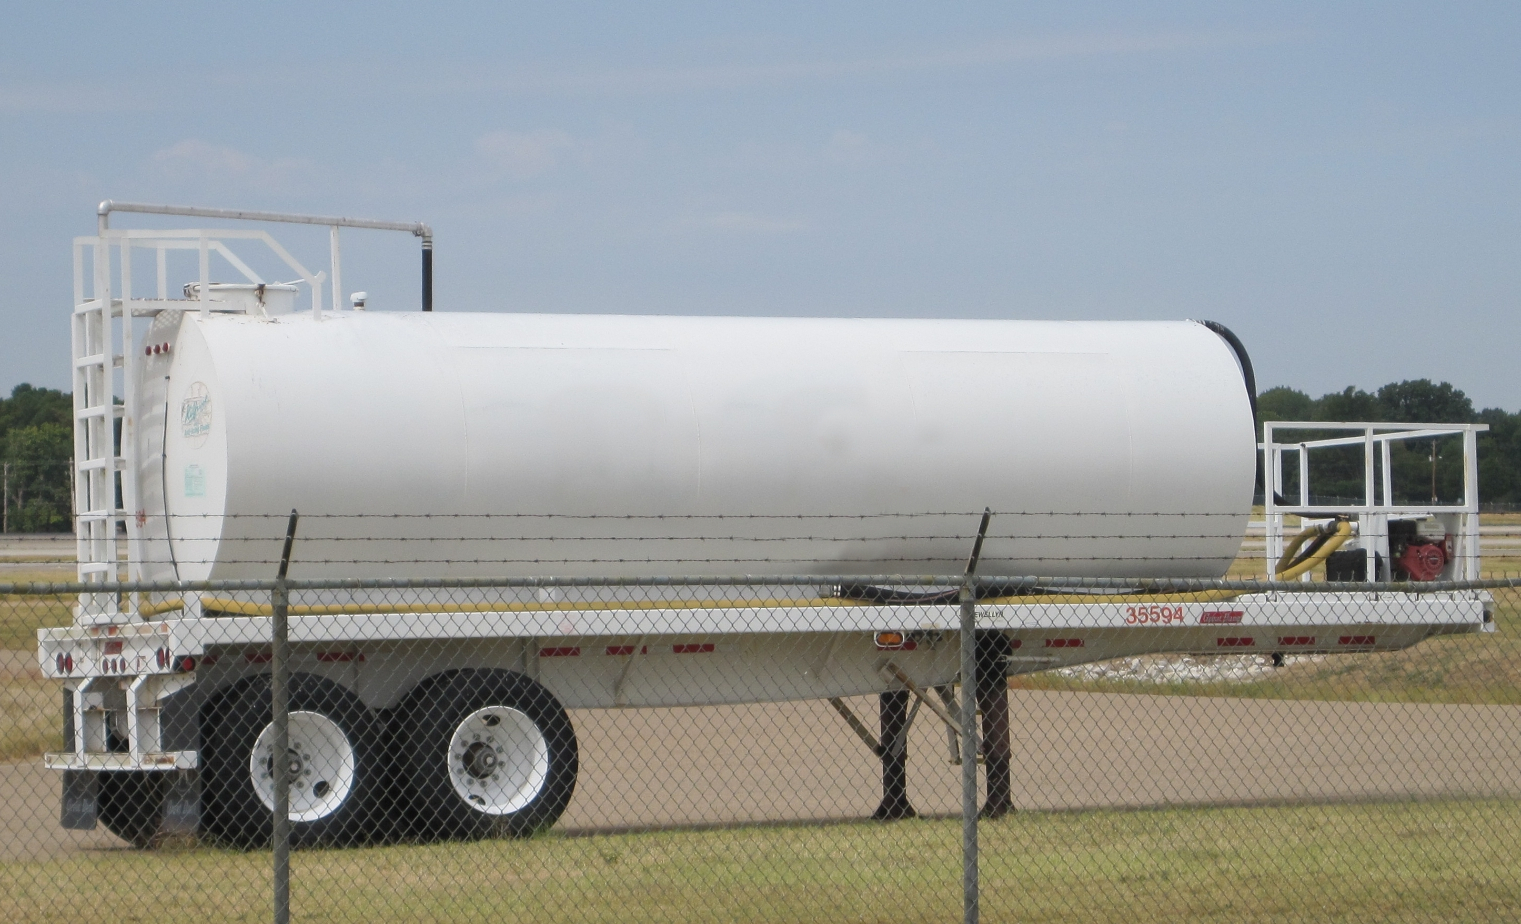
\includegraphics[height=0.31\textwidth]{images/fueltank.jpg}
			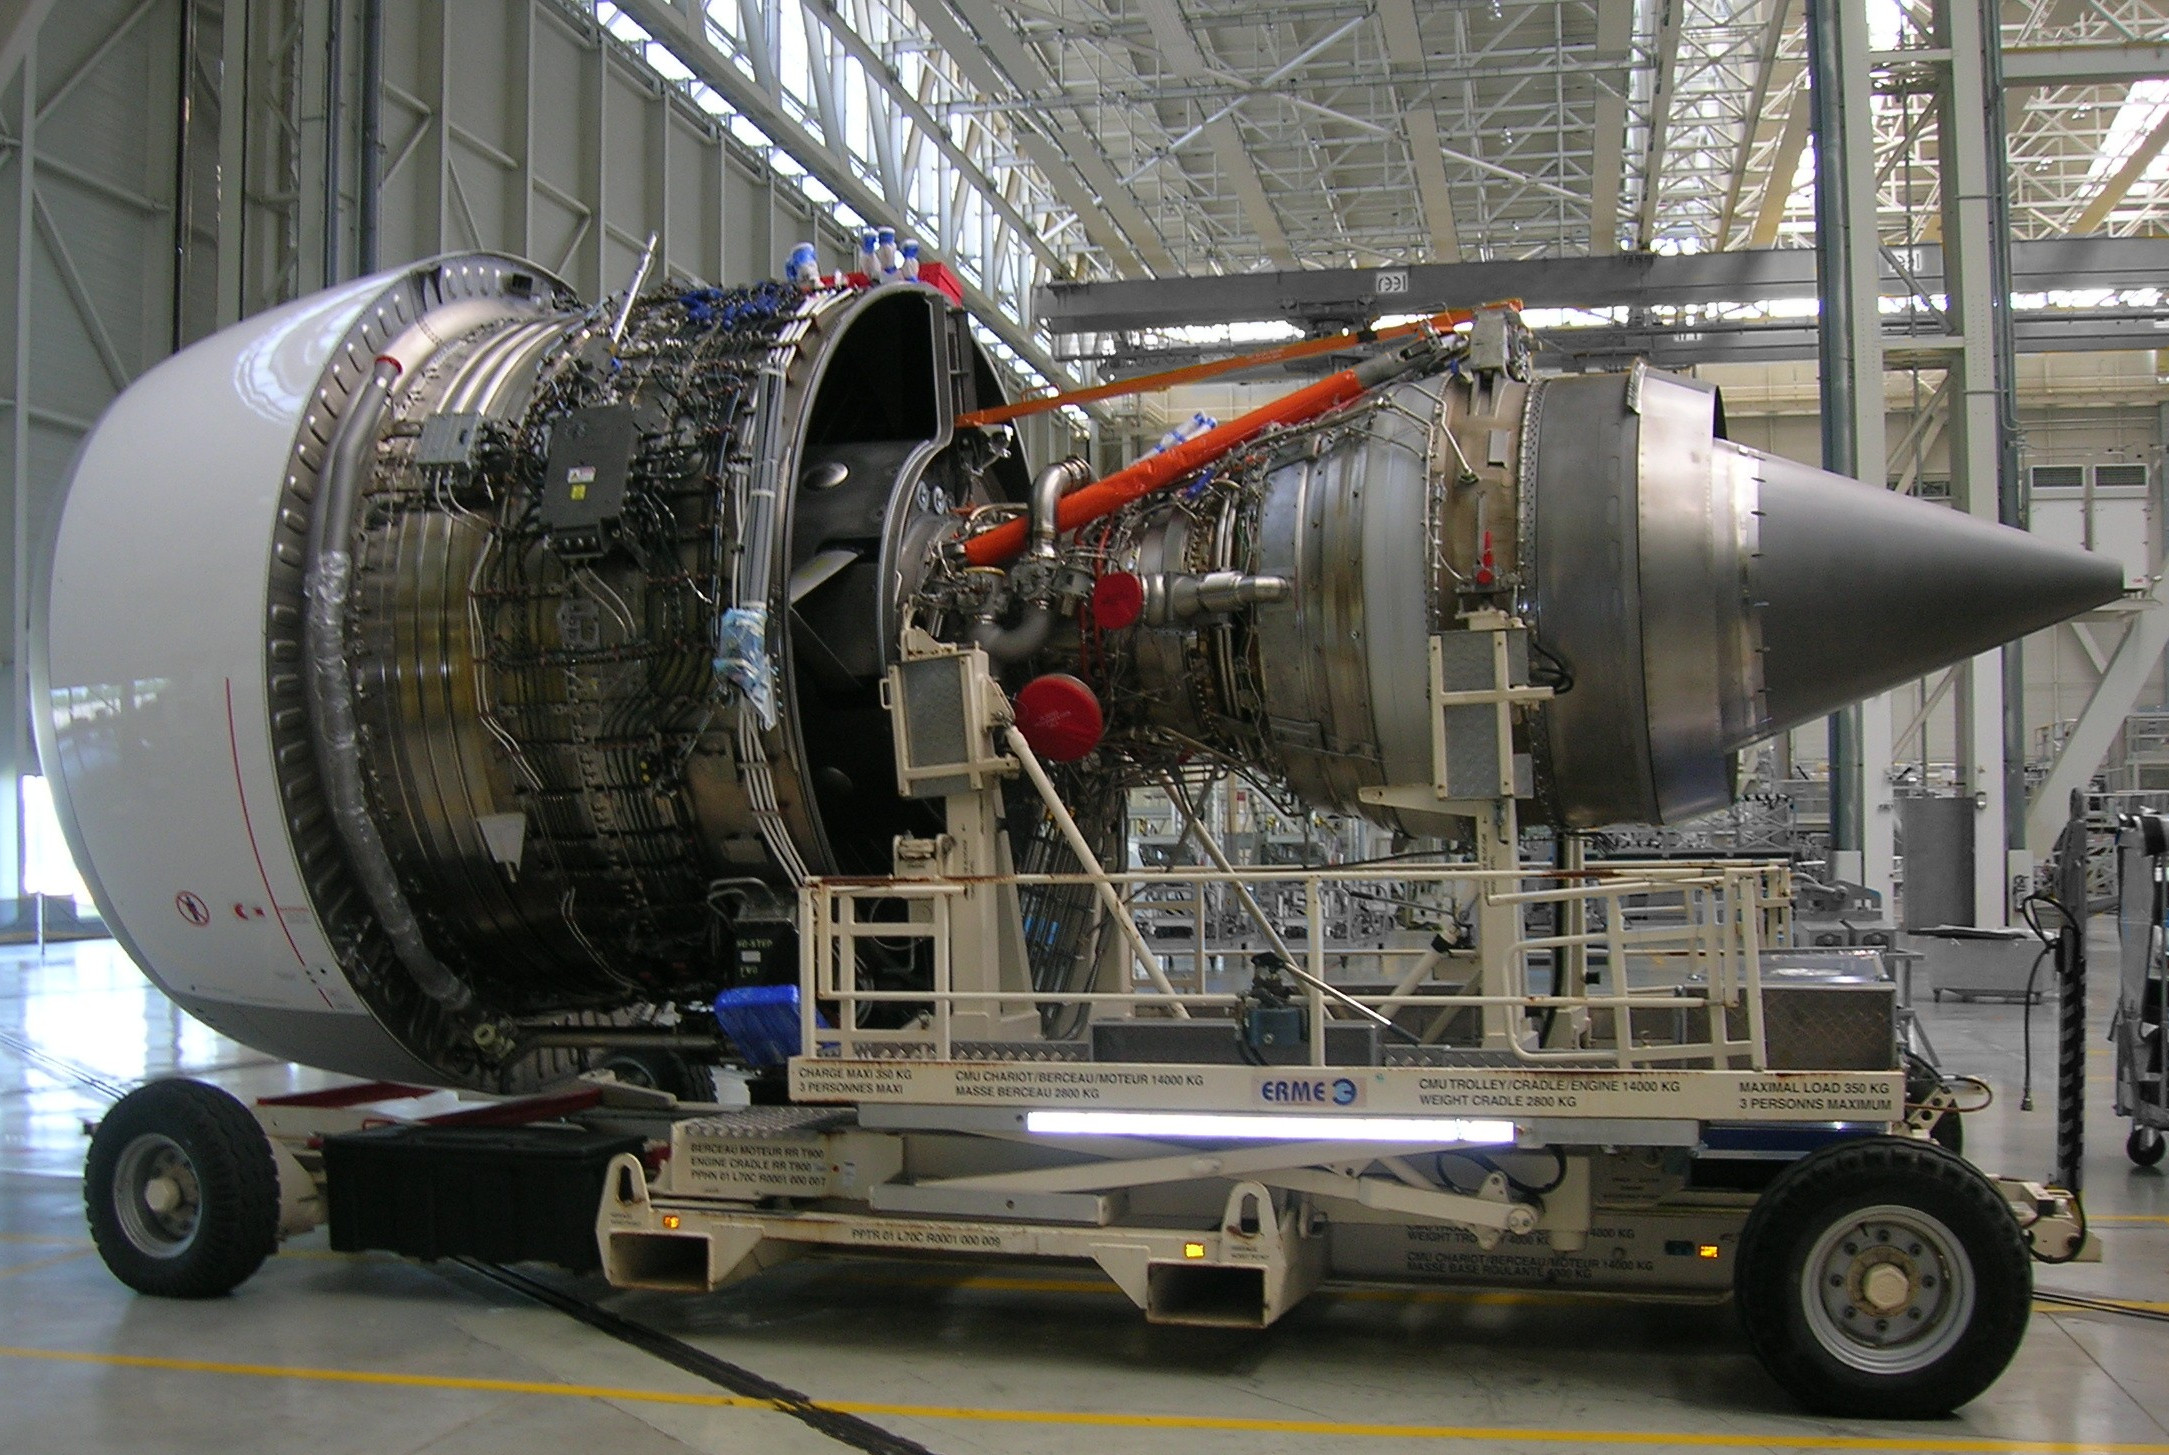
\includegraphics[height=0.31\textwidth]{images/trent900.jpg}
			\end{center}
			\supercaption{Une remorque, de puissance nulle ($\dot Q = \SI{0}{\watt}$) mais capable de restituer beaucoup d’énergie. La combustion de~\SI{20}{\tonne} de kérosène dégage environ $Q = \SI{900}{\giga\joule}$ sous forme de chaleur ; \\
				Un turboréacteur à soufflante \textit{Trent 900}, de très grande puissance (capable de fournir $\dot W = \SI{20}{\mega\watt}$ à un avion de ligne) mais dépourvu d’énergie (\SI{0}{\joule}).}{Photo turboréacteur dérivée d’\wcfile{Airbus_Lagardère_-_Trent_900_engine_MSN100_(2).JPG}{une photo} \cczero par \wcu{Dr Brains}\\ Photo remorque dérivée d’\wcfile{FedEx_Express_fuel_tank_trailer_at_Memphis_International_Arirport.jpg}{une photo} \ccby Thomas R Machnitzki}
			\label{fig_energie_puissance}
		\end{figure}
		
		D’autres unités sont souvent utilisées, comme le cheval-vapeur%
			\footnote{Un cheval-vapeur correspond approximativement à la puissance que peut fournir sous forme de travail un cheval puissant en plein effort. Nous devons la création de cette unité à… James Watt (\S\ref{ch_cheval_vapeur}). Attention, il existe plusieurs définitions incompatibles de l’unité \textit{cheval}. L’\cref{eq_equivalence_cheval} correspond à la norme \textsc{din} 66036 utilisée dans l’industrie automobile.} :
		\begin{equation}
			\SI{1}{ch_M} = \SI{735,5}{\watt}
			\label{eq_equivalence_cheval}
		\end{equation}

		Nous noterons les puissances en apposant un point au-dessus du symbole de l’énergie ; ainsi on note $\dot{E}$ \ une puissance (par exemple mécanique) apportant une quantité d’énergie $E$ chaque seconde.

		Dans le langage courant, le terme \textit{puissance} est utilisé pour quantifier \textit{la puissance maximale utile} d’un système. Par exemple, une automobile dont on dit qu’elle est «~de puissance 100~chevaux~» a un moteur capable de lui fournir, pendant quelques instants, une puissance de $\dot W_{\text{méca.}} = \SI{100}{ch}$ -- mais pour cela, le moteur reçoit environ $\dot Q_{\text{combustion}} = \SI{300}{ch}$ sous forme de chaleur. En outre, sur route, la puissance mécanique moyenne fournie par le moteur ne dépasse probablement pas~\SI{20}{ch}.

	\subsection{L’énergie et la puissance massiques}
	\label{ch_valeurs_spécifiques}

		Dans de nombreuses applications en thermodynamique, il est intéressant de quantifier les transferts énergétiques indépendamment de la quantité de masse à l’intérieur de la machine.

		Par exemple, si l’on souhaite comparer le \emph{fonctionnement} du moteur d’une moto et de celui d’un camion, il sera judicieux de diviser chacun des transferts énergétiques (pendant la compression, la combustion, la détente) par la quantité d’air dans les cylindres, pour s’affranchir des effets d’échelle.

		À cet effet, nous utilisons des grandeurs dites \vocab{spécifiques} (dites parfois \vocab{massiques}) ; et nous les noterons en minuscules.

		\begin{description}
		
			\item[L’énergie spécifique] (parfois appelée énergie massique), se mesure en \si{joules} \si{par} \si{kilogramme}~(\si{\joule\per\kilogram}) :
				\begin{equation}
					e \equiv \frac{E}{m}
				\label{def_énergie_spécifique}
				\end{equation}
				\begin{equationterms}
					\item où \tab $e$ \tab est l’énergie spécifique (\si{\joule\per\kilogram}),
					\item 	\tab $E$ \tab l’énergie (\si{\joule}),
					\item et \tab $m$	\tab la masse du système que l’on étudie (\si{\kilogram}).
				\end{equationterms}
		
				\begin{anexample}
					Un injecteur d’essence dans un moteur de voiture doit fournir une quantité de chaleur spécifique $q_{\text{comb.}} = \SI{300}{\kilo\joule\per\kilogram}$ quelle que soit la quantité d’air dans le cylindre. Quelle sera l’énergie fournie lorsque $m_\text{air} = \SI{0,5}{\kilogram}$ et lorsque $m_\text{air} = \SI{1}{\kilogram}$ ?
		
					\begin{answer}Il faudra $Q_{\text{comb.}1} = m_1 q_{\text{comb.}} = \num{0,5} \times \num{300e3} = \num{150e3} = \SI{150}{\kilo\joule}$ dans le premier cas, et $Q_{\text{comb.}2} = m_2 q_{\text{comb.}} = \SI{300}{\kilo\joule}$ dans le second.\end{answer}
					\end{anexample}

		\item[La puissance spécifique] (parfois également appelée puissance massique), a les mê\-mes unités : on divise des \si{watts} (\si{joules} \si{par} \si{seconde}) par un débit de masse (\si{kilos} \si{par} \si{seconde}).
			\begin{equation}
				e \equiv \frac{\dot{E}}{\dot{m}}
				\label{def_puissance_spécifique}
			\end{equation}
			\begin{equationterms}
				\item où \tab $e$ 		\tab est la puissance spécifique (\si{\joule\per\kilogram}),
				\item 	\tab $\dot{E}$ \tab la puissance (\si{\watt}),
				\item et \tab $\dot{m}$ \tab le débit de masse traversant le système (\si{\kilogram\per\second}).
			\end{equationterms}

			\begin{anexample}
				Une chambre de combustion dans un turboréacteur doit fournir une quantité de chaleur spécifique $q_{\text{comb.}} = \SI{300}{\kilo\joule\per\kilogram}$ quel que soit le débit d’air traversant le moteur. Quelle sera la puissance fournie lorsque $\dot{m}_\text{air} = \SI{0,5}{\kilogram\per\second}$ et lorsque $\dot{m}_\text{air} = \SI{1}{\kilogram\per\second}$ ?
		
				\begin{answer}Il faudra une puissance $\dot{Q}_{\text{comb.}1} = \dot{m}_1 q_{\text{comb.}} = \num{0,5} \times \num{300e3} = \num{150e3} = \SI{150}{\kilo\watt}$ dans le premier cas, et $\dot{Q}_{\text{comb.}2} = \dot{m}_2 q_{\text{comb.}} = \SI{300}{\kilo\watt}$ dans le second.
					\begin{remark}La puissance $\dot{Q}$ et le débit de masse $\dot{m}$ sont notés avec un point (débit dans le temps) mais pas la puissance spécifique $q$, qui est mesurée en \si{\joule\per\kilogram} comme la chaleur spécifique.\end{remark}\end{answer}
			\end{anexample}
		
		\end{description}

		Il faut noter qu’en pratique l’adjectif «~spécifique~» ou «~massique~» est souvent omis même si la quantité (ou le débit) de masse est inconnue, et que beaucoup d’auteurs n’utilisent pas la notation en minuscules.
		
\section{L’énergie mécanique}
\label{ch_energie_mecanique}

	L’étudiant/e n’aura aucun mal à quantifier l’\vocab{énergie cinétique} :
	\begin{equation}
	E_{c} = \frac{1}{2} \ m \ C^2
	\label{eq_énergie_cinétique}
	\end{equation}
	\begin{equationterms}
		\item où \tab $E_{c}$ 	\tab est l’énergie cinétique (\si{\joule}),
		\item 	\tab $m$ 		\tab la masse du corps (\si{\kilogram}),
		\item et	\tab $C$			\tab la vitesse (\si{\metre\per\second}).
	\end{equationterms}

	On définit bien sûr de façon correspondante l’\vocab{énergie cinétique spécifique} :
	\begin{equation}
		e_{c} \equiv \frac{E_{c}}{m} = \frac{1}{2} \ C^2
		\label{def_énergie_cinétique_spécifique}
	\end{equation}


	En thermodynamique, nous nous intéressons surtout aux variations d’énergie des fluides dans les machines. L’énergie cinétique des gaz varie de façon négligeable dans les moteurs à pistons/cylindres ; mais elle joue le rôle principal au sein des turboréacteurs, comme nous le verrons au \coursdix.

	L’expression de l’\vocab{énergie potentielle d’altitude} ne devrait pas non plus faire sourciller l’étudiant/e :
	\begin{IEEEeqnarray}{rCl}
		E_p 	& = & m \ g \ z	\\
		e_p 	&\equiv& \frac{E_p}{m}  = g \ z
		\label{eq_énergie_potentielle}
	\end{IEEEeqnarray}
	\begin{equationterms}		
		\item où \tab $g$ \tab est l’accélération gravitationnelle (usuellement \SI{9,81}{\metre\per\second\squared}),
		\item et \tab $z$ \tab l’altitude par rapport au point de référence (\si{\metre}).
	\end{equationterms}

	Nous montrerons que dans les machines, la variation de l’énergie potentielle d’altitude de l’air est toujours négligeable ; et que c’est souvent aussi le cas pour l’eau.

	Énergie cinétique et potentielle d’altitude sont souvent rassemblées en un seul terme, nommé \vocab{énergie mécanique} :
	\begin{equation}
		e_{m} \equiv e_{c} + e_p = \frac{1}{2}C^2 + g \ z
		\label{def_énergie_mécanique_spécifique}
	\end{equation}

		\begin{anexample}
			Un/e cycliste descend une route de montagne en roue libre. À un point d’altitude~\SI{540}{\metre}, sa vitesse est de~\SI[per-mode = symbol]{10}{\kilo\metre\per\hour}. Quelques instants plus tard, en passant un point d’altitude~\SI{490}{\metre}, sa vitesse est de~\SI[per-mode = symbol]{45}{\kilo\metre\per\hour}. La masse du/de la cycliste et de son équipement est de~\SI{70}{\kilogram}.
			
			Quelle quantité d’énergie a-t-il/elle dissipé sous forme de frottements ?
			
				\begin{answer}
					L’énergie mécanique du/de la cycliste a varié de $\Delta E_m = E_{m 2} - E_{m 1} = m (e_{m 2} - e_{m 1}) = m (g z_2 - g z_1 + \frac{1}{2} C_2^2 - \frac{1}{2} C_1^2) =  m \left[ g (z_2 - z_1) + \frac{1}{2} (C_2^2 - C_1^2)\right] = 70 \left[ \num{9,81} (490 - 540) + \frac{1}{2} \left( \left(\frac{\num{45e3}}{\num{3600}}\right)^2 - \left(\frac{\num{10e3}}{\num{3600}}\right)^2\right) \right] = 70 \left[ \num{-490,5} + \num{74,3} \right] = \SI{-2,91e4}{\joule} = \SI{-29,1}{\kilo\joule}$.
					
					Le/la cycliste a donc perdu~\SI{29,1}{\kilo\joule} d’énergie mécanique. Cette quantité a été transmise à l’atmosphère, sous forme de turbulence et de chaleur, et aux roulements et pneus du vélo, sous forme de chaleur.
						\begin{remark}Les variations d’énergie peuvent très bien être négatives. L’énergie cinétique est par contre toujours positive. \end{remark}
						\begin{remark}Le passage du vélo dans l’air provoque des agitations observables à l’échelle macroscopique que nous nommons \vocab{turbulence}. Après un court laps de temps, cette énergie cinétique s’est dissipée à l’échelle microscopique, de sorte que l’on a réchauffé l’atmosphère. \end{remark}
				\end{answer}
		\end{anexample}



\section{Le travail}
\label{ch_travail_fdl}

	Le \vocab{travail} est un transfert d’énergie. Un objet fournit un travail (et perd ainsi de l’énergie) lorsqu’il exerce une force le long d’un déplacement. En mécanique, ce travail est quantifié à l’aide de vecteurs :
	\begin{equation}
		W \equiv \vec F \cdot \vec l
		\label{def_travail}
	\end{equation}
	\begin{equationterms}		
		\item où \tab $W$ 		\tab est le travail (\si{\joule}),
		\item 	\tab $\vec F$ 	\tab le vecteur représentant la force (de norme $F$ en \si{\newton}),
		\item et \tab $\vec l$ 	\tab le vecteur représentant le déplacement effectué (de norme $l$ en \si{\metre}).
	\end{equationterms}

	En thermodynamique, nous allons utiliser cette \cref{def_travail} pour quantifier le travail effectué par des fluides. Pour cela nous allons apporter trois contraintes :
	
	\begin{itemize}
		\item Nous mesurerons le déplacement \emph{avec la longueur de l’objet qui fournit le travail} ;
		\item Nous ne nous intéresserons qu’aux cas où les vecteurs $\vec F$ et $\vec l$ sont colinéaires ;
		\item Nous tiendrons compte du fait que $\vec F$ peut varier en fonction de $\vec l$.
	\end{itemize}


	Avec ces trois contraintes l’\cref{def_travail} devient :
		\begin{equation*}
		W_\fromatob = \int_\A^\B {\diff W} = \int_\A^\B {\vec F \cdot \diff \vec l}
		\end{equation*}

	Comme $\diff \vec l$ est mesuré à partir de la longueur de l’objet qui travaille, $\diff l$ sera négatif lorsque $W$ est positif (l’objet recevant alors du travail, en voyant sa longueur diminuer). Enfin, $\vec F$ étant dans notre cas toujours colinéaire à $\diff \vec l$, nous pouvons écrire :
		\begin{equation}
		W_\fromatob = -\int_\A^\B {F \diff l}
		\label{eq_travail_fdl}
		\end{equation}
	\begin{equationterms}		
		\item où \tab $W_\fromatob$ 	\tab est le travail effectué entre deux points A et B (\si{\joule}),
		\item 	\tab $F$ 				\tab est la force (\si{\newton}),
		\item et \tab $\diff l$ 		\tab est la variation infinitésimale de la longueur de l’objet considéré (\si{\metre}).
	\end{equationterms}

	Sur un graphique représentant la force en fonction de la distance, ce travail $W_\fromatob$ est représenté par la surface sous la courbe de A à B (\cref{fig_force-déplacement-aire}). La forme de la courbe, c’est-à-dire la relation $F_{(l)}$ entre $F$ et $l$ au fur et à mesure de l’évolution, déterminera la quantité $W_\fromatob$.
	
	\begin{figure}
	\begin{center}
		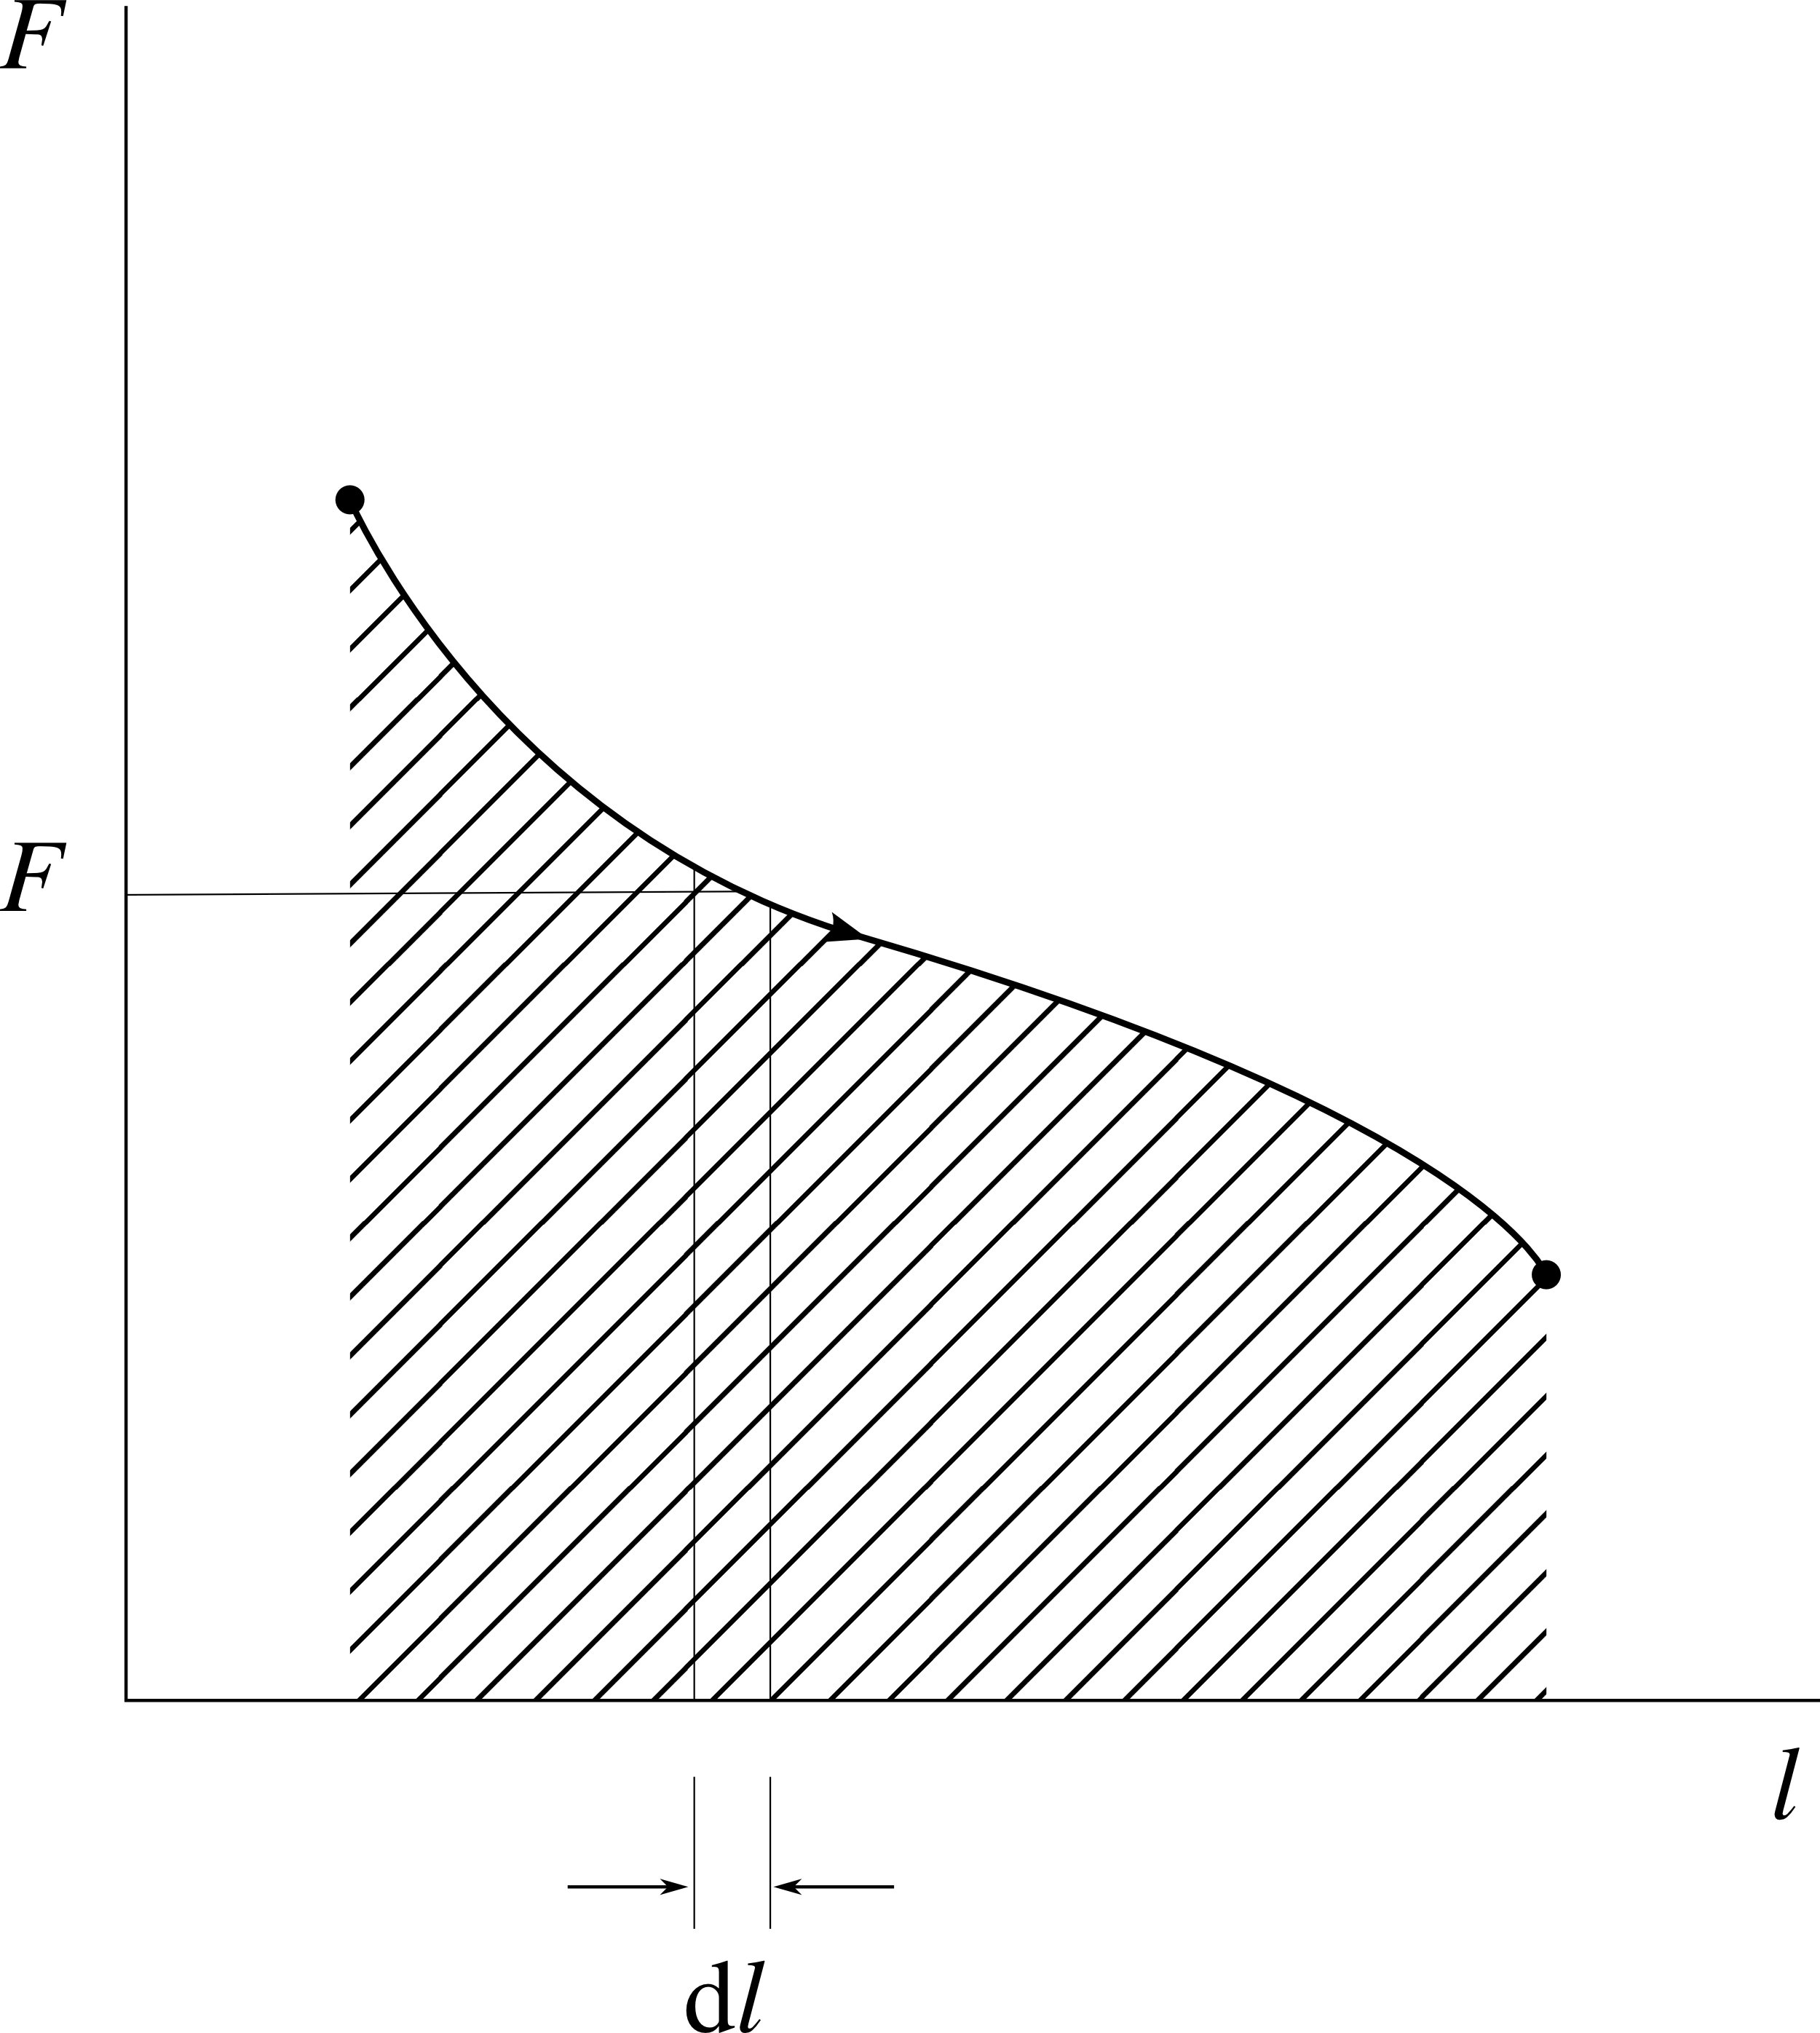
\includegraphics[width=\didacticpvdiagramwidth]{images/fl.png}
	\end{center}
	\supercaption{Le travail fourni par un objet peut être visualisé avec l’aire sous la courbe force-déplacement. Dans le cas montré ici, l’objet voit sa longueur $l$ augmenter, et le travail sera négatif (fourni par l’objet).}{schéma \cczero \oc}
	\label{fig_force-déplacement-aire}
	\end{figure}

		\clearfloats
		\begin{anexample}
			Un ressort est comprimé depuis une longueur de~\SI{30}{\centi\metre} jusqu’à une longueur de~\SI{5}{\centi\metre}. Le ressort est tel qu’il exerce une force (en \si{newtons}) indépendante de sa longueur et égale à
				\begin{equation*}
					F_{(l)} = \SI{6e3}{\newton}
				\end{equation*}
			Quelle est l’énergie fournie au ressort sous forme de travail pendant la compression ?
				
				\begin{answer}
					Le transfert de travail s’obtient avec l’\cref{eq_travail_fdl}, en prenant soin de poser les bornes en unités \textsc{si} :
					$ W_\fromatob = - \int_\A^\B F_{(l)} \diff l = - \int_\A^\B \num{6e3} \diff l = - \num{6e3} \int_\A^\B \diff l = - \num{6e3} \left[l\right]_{l_\A}^{l_\B } = -\num{6e3} (\num{0,05} - \num{0,3}) = \SI{+1,5e3}{\joule} = \SI{+1,5}{\kilo\joule}.$
						\begin{remark} Le signe du travail transféré est positif : le ressort a \emph{reçu} de l’énergie. Cela ne nous surprend pas : sa longueur a diminué, pendant qu’il se faisait comprimer.\end{remark}
						\begin{remark} Les ressorts possédant une telle caractéristique (indépendante de leur longueur) sont souvent des ressorts en ruban, comme ceux alimentant les montres mécaniques. \end{remark}
				\end{answer}
		\end{anexample}

		\begin{anexample}
			Un autre ressort est comprimé depuis une longueur de~\SI{30}{\centi\metre} jusqu’à une longueur de~\SI{5}{\centi\metre}. Il est tel qu’il exerce une force (en \si{\newton}) liée à sa longueur $l$ (en~\si{\metre}) par la relation :
				\begin{equation*}
					F_{(l)} = \num{9e3} - \num{14e3} \ l
				\end{equation*}
			Quelle est l’énergie fournie au ressort sous forme de travail pendant la compression ?
				
				\begin{answer}
					Le travail effectué s’obtient toujours avec l’\cref{eq_travail_fdl}, dont l’intégrale est à peine plus complexe :
					$ W_\fromatob = - \int_\A^\B (\num{9e3} - \num{14e3} l) \diff l = - \left[\num{9e3} \ l - \frac{1}{2} \num{14e3} \ l^2\right]_{l_\A}^{l_\B } = -\num{e3} \left[9 l - 7 l^2\right]_{\num{0,3}}^{\num{0,05}} =  -\num{e3} (\num{0,4325} - \num{2,07}) = \SI{+1,6375e3}{\joule} = \SI{+1,638}{\kilo\joule}.$
						\begin{remark} Les ressorts possédant une telle caractéristique (force proportionnelle à la distance) sont souvent à spires régulières. \end{remark}
				\end{answer}
		\end{anexample}

		\begin{anexample}
			Un autre ressort est comprimé depuis une longueur de~\SI{30}{\centi\metre} jusqu’à une longueur de~\SI{5}{\centi\metre}. Il est tel qu’il exerce une force (en~\si{\newton}) liée à sa longueur $l$ (en~\si{\metre}) par la relation :
				\begin{equation*}
					F_{(l)} = \num{14e3} - \num{12e3} \ l^{\num{0,3}}
				\end{equation*}
			Quelle est l’énergie fournie au ressort sous forme de travail pendant la compression ?
				
				\begin{answer}
					Le travail effectué s’obtient encore et toujours avec l’\cref{eq_travail_fdl},\\
					$ W_\fromatob = - \int_\A^\B (\num{14e3} - \num{12e3} \ l^{\num{0,3}} ) \diff l = - \num{e3} \left[\num{14} \ l - \frac{1}{\num{0,3}+1} 12 \ l^{\num{0,3}+1} \right]_{\num{0,3}}^{\num{0,05}} = -\num{e3} \ (\num{0,5121} - \num{2,2703}) = \SI{+1,7582e3}{\joule} = \SI{+1,758}{\kilo\joule}.$
						\begin{remark} Les ressorts possédant une telle caractéristique sont à spires progressives : très souples au départ, mais augmentant rapidement en dureté. Ils sont souvent utilisés dans les suspensions d’automobiles. Nous verrons au \coursdeux que les gaz on une caractéristique similaire.\end{remark}
				\end{answer}
		\end{anexample}



\section{La chaleur}

	\subsection{La température}
	\label{ch_définition_température_cours1}

		Nous définissons temporairement la \vocab{température} comme étant le potentiel d’un corps à fournir ou recevoir de la chaleur.

		La température d’un corps est une grandeur qui indique son niveau d’excitation interne. Plus ses molécules possèdent d’énergie cinétique, avec des vitesses de direction différente, et plus sa température sera grande.

		Lorsque les molécules constituant un corps sont parfaitement immobiles les unes par rapport aux autres, le corps n’a plus de vibration interne : cet état définit la température zéro. À l’inverse, l’échelle de température est ouverte vers l’infini. On ne définit pas de point de température maximale.

		On ne peut pas mesurer simplement «~l’énergie cinétique moyenne des molécules~» d’un corps et il s'ensuit qu’il est très difficile de définir rigoureusement une échelle de température (par exemple, ce que représente une température «~deux fois plus grande~»). Nous reviendrons sur la notion même de température au \coursquatre et nous la définirons tout à fait au \courssept. Nous admettrons, dans cette attente, la définition donnée plus haut.

		La température se mesure en \si{kelvins} (\si{\kelvin}), sur une échelle créée pour les besoins de la thermodynamique et fort peu modestement qualifiée d’\vocab{absolue}.

		L’étudiant/e aura probablement l’habitude d’utiliser une échelle en \si{degrés} \si{Celsius}~(\si{\degreeCelsius}). Elle précède l’échelle absolue en \si{kelvins}, mais a été habilement redéfinie et synchronisée avec cette dernière en 1848%
			\footnote{Nous aurons l’occasion d’étudier ce magnifique tour de passe-passe au \courssept.}%
		. Il suffit de soustraire 273,15 unités à une température absolue (en \si{kelvins}) pour lire une température en \si{degrés} \si{Celsius} :
		\begin{equation}
			T(\si{\degreeCelsius})\ \equiv \ T(\si{\kelvin}) - 273,15
			\label{def_température_kelvins_celsius}
		\end{equation}

		Les puristes remarqueront que l’unité est nommée \si{kelvin} et non «~degré Kelvin~». Quelques températures indicatives sont recensées dans le \cref{tab_temperatures}.

		\begin{table}
		\centering
		\renewcommand{\tabcolsep}{0.8em}
		\renewcommand{\arraystretch}{1.3}
		\sisetup{table-number-alignment=center-decimal-marker} %in this table, we don’t care about alignment
		\begin{footnotesize}
		\begin{spacing}{1}
		\begin{innersidebox}
		\begin{tabularx}{15.5cm}{@{}S@{}S|p{8.5cm}@{}} % the @{something} kills the inter-column space and replaces it with "something"
% last column width has to be set manually ; will break if margins change.
% L column in tabulary solves this but tabulary precludes using arydshln
			\toprule
			{\si{kelvins}} & {\si{degrés} \si{Celsius}} & ~ 	\\ % accolades allow escaping from the S column number alignment rules
			\midrule
			0		& -273,15	&	Zéro absolu (par définition) \\
			10e-11	& -273.1499999999	& Température la plus basse jamais atteinte (quelques particules seulement) \\
			4,22	& -268,93	& Ébullition de l’hélium à pression atmosphérique \\
			44	& -229		& Température moyenne de la surface de Pluton* \\
			184	& -89,4		& Température atmosphérique minimale enregistrée sur Terre* \\
			273,15	& 0		& Fonte de l’eau à pression atmosphérique \\
			327	& 54		& Température atmosphérique maximale enregistrée sur Terre* \\
			373,15	& 100		& Ébullition de l’eau à pression atmosphérique \\
			400	& 127		& Température du nez d’un Concorde en croisière* \\
			483	& 200		& Four domestique ordinaire* \\
			485	& 210		& Auto-inflammation du carburant diesel* \\
			753	& 480		& Température des bords d’attaque d’un \wfd{Lockheed SR-71 Blackbird}{\textsc{sr}-71} en croisière* \\
			1100	& 830		& Feu de bois* \\
			1900	& 1600		& Température du bouclier d’une navette spatiale en rentrée atmosphérique* \\
			2500	& ~		& Filament d’une lampe à incandescence \\
			5000	& ~		& Fonte du diamant (à~\SI{12}{\giga\pascal}) \\
			5800	& ~		& Surface du soleil \\
			16e6	& ~		& Centre du soleil \\
			350e6	& ~		& Au sein de la déflagration d’une arme nucléaire \\
			3e9	& ~		& Cœur d’une grosse étoile à son dernier jour \\
			1e12	& ~		& Particules en collision au sein du RHIC \\
			1.417e32	& ~	& L’univers \SI{5,391e-44}{\second} après le Big Bang \\
			\hline
		\end{tabularx}
		\end{innersidebox}
		\end{spacing}
		\end{footnotesize}
		\caption{Quelques exemples de températures. Les astérisques dénotent une conversion approximative (liée à la précision des valeurs).}
		\sisetup{table-number-alignment=center} % back to setting specified in our stylesheet
		\label{tab_temperatures}
		\end{table}
		
		
	\subsection{La chaleur}
	
		\thermoquotebegin{O}
			Ces résultats sont inexplicables si nous considérons que la chaleur est une substance.\nolinebreak\makebox(18,5){\color{gray}\scalebox{2}{»}}\par\vspace{-0.3cm}\begin{flushright}James Joule, 1845\\\textit{On the Changes of Temperature Produced by the Rarefaction and Condensation of Air}~\cite{joule1845}\end{flushright}\vspace{-1em}
		%\thermoquoteend{James Joule, 1845}{\textit{On the Changes of Temperature Produced by the Rarefaction and Condensation of Air}~\cite{joule1845}}
		%\thermoquotebegin{O}
		\makebox(18,5){\color{gray}\scalebox{2}{«}}
			Ces circonstances […] nécessitent une comparaison entre travail et chaleur, qu’il nous faut effectuer en partant de l’hypothèse divergente que la production de travail est due non seulement à un changement dans la \emph{distribution} de la chaleur, mais aussi à une \emph{consommation} de celle-ci ; et inversément, que par la consommation de travail la chaleur puisse être \emph{produite}.
		\thermoquoteend{Rudolf Clausius, 1850}{\textit{Über die bewegende Kraft der Wärme und die Gesetze, welche sich daraus für die Wärmelehre selbst ableiten lassen} \mbox{\cite{clausius1850, clausius1850en, clausius1868fr1}}}

		Lorsque l’on met deux corps de températures différentes en contact, leurs températures ont tendance à s’égaliser au cours d’un transfert spontané d’énergie. Nous appelons cette forme d’énergie la \vocab{chaleur}.

		La chaleur, notée $Q$, est \textbf{une forme d’énergie} (mesurée en \si{joules}). À l’échelle macroscopique, c’est un transfert d’énergie sous forme chaotique. On peut le provoquer de plusieurs façons, dont les plus pertinentes pour l’ingénieur/e sont :

		\begin{itemize}
		
			\item la perte d’énergie interne d’un corps, par mise en contact avec un corps de température plus basse ;

			\item le frottement ;
			
			\item la disparition de masse au sein d’une réaction nucléaire ;
			
			\item la transformation d’énergie potentielle entre atomes, par réaction chimique (en particulier la combustion d’hydrocarbures avec l’oxygène atmosphérique).

		\end{itemize}
		
		De même que l’on note $Q$ la chaleur (\si{\joule}), on note $q$ la \vocab{chaleur spécifique} (\si{\joule\per\kilogram}).
		
		La notion de chaleur est très difficile à appréhender. On l’a longtemps crue être un fluide (le \textit{calorique}) de densité très faible, capable d’imprégner tous les matériaux. Cette théorie a été abandonnée au milieu du \textsc{xix}\ieme siècle, lorsque l’on a mis en évidence que \textit{la chaleur n’est pas conservée}, c’est-à-dire qu’elle a une capacité à disparaître ou apparaître. Par exemple, un moteur en marche reçoit de la chaleur (par combustion) mais il en rejette moins qu’il n’en a reçu. Il en transforme une partie en travail, que l’on utilise par exemple pour propulser un véhicule. \\
		À l’échelle microscopique (lorsque l’on considère le mouvement individuel des particules) les concepts de température et de chaleur sont plus difficiles encore à définir ; mais cela dépasse le domaine d’étude de cet ouvrage\footnote{Pour mieux définir les frontières entre les échelles macroscopique et microscopique dans la thermodynamique de l’ingénieur, les étudiants les plus rigoureux pourront par exemple consulter l’ouvrage d’Alexandre Watzky~\cite{watzky2007}. Richard Feynman~\cite{feynman1963, feynman1963fr} explore à plusieurs reprises ces changements d’échelle et leurs implications.}\nolinebreak.


	\subsection{La capacité thermique}
	\label{ch_capacite_thermique}

		Lorsque l’on fournit la même quantité de chaleur à deux corps différents, leur température peut augmenter de différente façon -- par exemple, il faut moins de chaleur pour augmenter de~\SI{1}{\degreeCelsius} la température d’un \si{kilogramme} d’acier que d’un \si{kilogramme} d’aluminium. Cette propension de la température à augmenter est nommée \vocab{capacité thermique} (ou \vocab{capacité calorifique}).

		On définit la capacité thermique massique d’un corps comme la quantité de chaleur nécessaire pour augmenter d’un \si{kelvin} la température d’un \si{kilogramme} de ce corps :
		\begin{equation}
			c\ \equiv \ \frac{\diff q}{\diff T} = \frac{1}{m} \frac{\diff Q}{\diff T}
			\label{eq_def_capacité_calorifique_massique}
		\end{equation}
		\begin{equationterms}
			\item où \tab $c$			\tab\tab est la \vocab{capacité thermique massique} du corps considéré (\si{\joule\per\kilogram\per\kelvin}),
			\item 	\tab $\diff q$ \tab est une quantité spécifique infinitésimale de chaleur (\si{\joule\per\kilogram}),
			\item et \tab $\diff T$ \tab est une variation infinitésimale de température (\si{\kelvin} ou \si{\degreeCelsius}).
		\end{equationterms}

		La capacité calorifique massique des solides est en général invariante. Par contre pour les fluides, que nous utilisons beaucoup dans les machines, ce n’est pas si simple :

		\begin{itemize}

			\item En faisant travailler un gaz (c’est-à-dire en le laissant pousser sur une paroi mobile), on augmente nettement sa capacité calorifique massique. Nous quantifierons ces propriétés au \coursquatre ;

			\item La capacité calorifique massique des liquides et vapeurs devient infinie~(!) pendant l’ébullition, qui a lieu sur une plage particulière de propriétés. Hors de cette plage, la capacité redevient finie mais elle varie avec la température. Nous décrirons ces comportements au \courscinq.

		\end{itemize}

		\begin{anexample}
			La capacité calorifique massique de l’acier solide est constante (indépendante de la température) et a pour valeur $c_{\text{acier}} = \SI{475}{\joule\per\kilogram\per\kelvin}$.
			
			Combien faut-il de chaleur pour faire passer un bloc de~\SI{50}{\kilogram} d’acier depuis une température $T_\A = \SI{5}{\degreeCelsius}$ jusqu’à une température $T_\B = \SI{18}{\degreeCelsius}$ ?
				\begin{answer}
					Nous utilisons la définition \ref{eq_def_capacité_calorifique_massique} pour écrire, dans le cas général :
						\begin{IEEEeqnarray*}{rCl}
							c_{\text{acier}} 				&=& \frac{1}{m_{\text{acier}}} \frac{\diff Q}{\diff T}\\
							\diff Q 							&=& c_{\text{acier}} \ m_{\text{acier}} \diff T\\
							Q_\fromatob						&=& \int_\A^\B m_{\text{acier}} \ c_{\text{acier}} \diff T
						\end{IEEEeqnarray*}
					Comme la capacité $c_{\text{acier}}$ est indépendante de $T$ cette intégrale devient simplement :
					$ Q_\fromatob = m_{\text{acier}} \ c_{\text{acier}} \int_\A^\B \diff T = m_{\text{acier}} \ c_{\text{acier}} (T_\B - T_\A ) = 50 \times 475 \times (18 - 5) = \SI{+3,0875e5}{\joule} = \SI{+308,8}{\kilo\joule}$.
						\begin{remark}Pendant l’intégration, $\int_\A^\B \diff T$ devient $\Delta T$ (une différence de température), tandis que $\int_\A^\B \diff Q$ devient seulement $Q_\fromatob$ (un transfert entre deux états). La chaleur n’est pas «~diminuée~», elle est transmise. Dans cet ouvrage, lorsque nous quantifions les transferts d’énergie, nous convenons d’en rendre le signe explicite.\end{remark}
						\begin{remark}Une conversion des deux températures en \si{kelvins} n’aurait pas changé la valeur du $\Delta T$. Le résultat serait bien sûr identique.\end{remark}
						\begin{remark}Avec une résistance électrique de la puissance d’un radiateur domestique ordinaire (\SI{2}{\kilo\watt}), il faudrait $\Delta t = \frac{Q_\fromatob}{\dot Q} = \frac{\num{308,8e3}}{\num{2e3}} = \SI{154}{\second}$ pour réchauffer l’acier, soit un peu plus de deux minutes. Nous verrons au \coursquatre que l’air à pression constante a une capacité calorifique massique trois fois plus grande que celle de l’acier.\end{remark}
				\end{answer}
		\end{anexample}


\section{Le chaud et le froid}

	Nous terminons ce chapitre en re-visitant quelques termes de langage courant tels que nous les comprenons en thermodynamique :

		\begin{description}

			\item \textit{Le chaud} --- Pour nous, «~chaud~» n’est pas une propriété des corps : plutôt que «~cet objet est chaud~» nous dirons qu’il est à haute température. Plutôt que «~cet objet s’échauffe/se refroidit~» nous dirons que sa température augmente ou diminue.\\
				Dans le langage courant, les expressions comme «~il fait chaud~» ou «~les grandes chaleurs~» font également allusion à la température.
			
			\item \textit{Chauffer} --- Pour nous, «~chauffer~» c’est fournir de la chaleur. On peut «~chauffer~» un corps pendant que sa température chute. On peut également faire augmenter la température d’un corps sans lui apporter de chaleur (\cref{fig_chauffer_refroidir}).

		\begin{figure}
			\begin{center}
			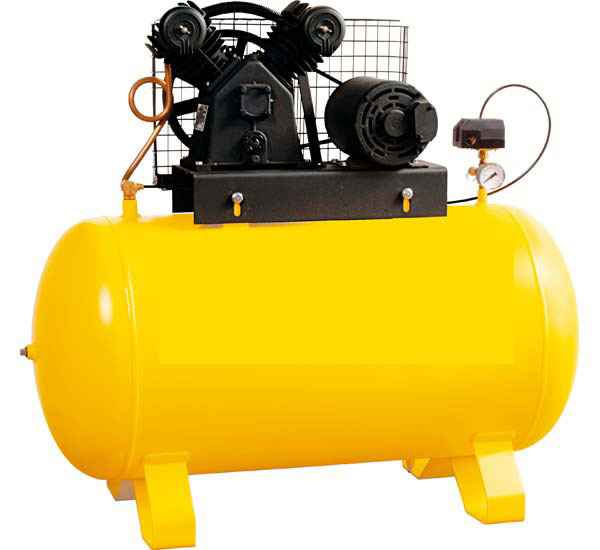
\includegraphics[height=0.38\textwidth]{images/air_piston_compressor.jpg}
			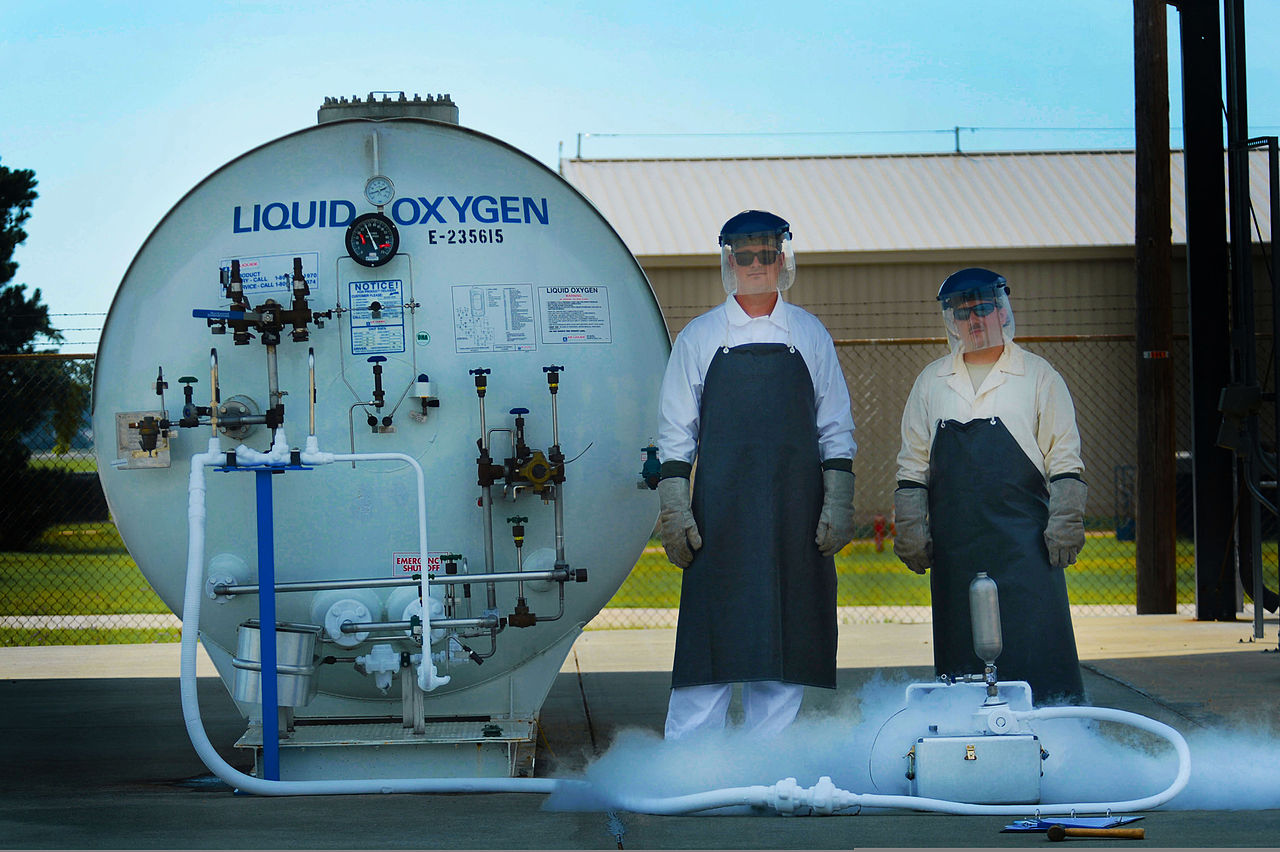
\includegraphics[height=0.38\textwidth]{images/liquid_oxygen_expansion.jpg}
			\end{center}
			\supercaption{Lorsqu’il est comprimé dans un compresseur, l’air perd de la chaleur au travers des parois et des aubes des cylindres ; et pourtant sa température augmente.\\
			À l’inverse, lorsqu’il est détendu dans une soupape, l’oxygène liquide reçoit de la chaleur de l’atmosphère (comme le mettent en évidence la condensation et le gel de l’eau atmosphérique sur les tuyaux) ; et pourtant sa température chute.}{\wcfile{Compressor3.jpg}{Photo compresseur} \ccbysa Fábio Teixeira\\ \wcfile{U.S. Air Force Tech. Sgt. Jason Powers, left, a noncommissioned officer in charge with the 20th Logistics Readiness Squadron (LRS), and Staff Sgt. Adam Rozell, a fixed facilities supervisor with the 20th LRS 140626-F-SX095-017.jpg}{Photo oxygène liquide} \pd Jensen Stidham / USAF}
			\label{fig_chauffer_refroidir}
		\end{figure}
			
			\item \textit{Le froid} --- Pour nous, la sensation de «~froid~» indique une faible température. Nous ne considérerons pas «~le froid~» comme étant quelque chose que l’on peut fabriquer ni mesurer. Nous dirons plutôt que nous prélevons de la chaleur d’un corps (par exemple, un réfrigérateur prend de la chaleur à un aliment tiède).
			
			\item \textit{Le feu} --- Le feu est le nom donné au dégagement de lumière (rayonnement électromagnétique) par un gaz à haute température. En thermodynamique, le «~feu~» n’a aucune propriété particulière. Il s’agit pour nous de la même chaleur qu’elle soit dégagée par combustion de bois, de kérosène, par frottement dans un frein, ou par une réaction nucléaire. Seule compte au final la température à laquelle elle est transmise !
			\end{description}

				\thermoquotebegin{o}
					Le principe à suivre pour construire une échelle de température peut tout d’abord paraître évident, puisqu’il peut apparaître qu’un thermomètre parfait ferait correspondre des ajouts de chaleur égaux à des élévations égales de température, mesurées par les graduations de son échelle. Il est toutefois désormais reconnu comme fait établi par l’expérience (par la variation des capacités calorifiques des corps) que la thermométrie sous ce précepte est impossible, et nous n’avons plus de principe sur lequel fonder une échelle thermométrique absolue.
				\thermoquoteend{William Thomson\\{\tiny(non encore couronné \textit{Baron Kelvin}…)}}{1848~\cite{kelvin1848}\vspace{2em}} %handmade vspace
				\vspace{-0.7em}~\vspace{-1.8em}%FIXME -- hack pour faire tenir la citation sur le côté
			\begin{description}
			\item \textit{Le thermomètre} --- Nous laissons à l’étudiant/e le loisir d’explorer le fonctionnement des \vocab{thermomètres} : comment peut-on \emph{savoir} dans l’absolu qu’une température est haute ou basse ?\\
				Nous nous contentons de remarquer que nous sommes nous-mêmes de très mauvais thermomètres : comme le corps humain s’efforce de se maintenir à température constante, nos sensations de «~chaud~» ou de «~froid~» sont intrinsèquement liées aux transferts de chaleur.

		\end{description}
		
	Même si ce vocabulaire nous place probablement au rang des scientifiques insociables relégués en bout de table, il nous équipe mieux pour affronter la suite, car au chapitre prochain, nous attaquons les \textit{systèmes fermés}.


\atstartofhistorysection
\onlyamphibook{\section[Un peu d’histoire : mesurer le degré de chaleur]{Un peu d’histoire :\\ mesurer le degré de chaleur}}
\onlyframabook{\section{Un peu d’histoire : mesurer le degré de chaleur}}
\label{ch_histoire_degre_chaleur_depondt}

\begin{center}\textit{Par Philippe Depondt\\ \begin{small}Université Pierre et Marie Curie, Paris\\ Contribution sous licence \ccbysa\end{small}}\end{center}

	Pour Aristote, au \textsc{iv}\ieme siècle avant J.C. en Grèce, le feu était l'un des quatre constituants de la matière avec l'eau, l'air et la terre. L'idée de mesurer quelque chose, le feu ou autre, c'est-à-dire de donner une valeur numérique à une grandeur, lui était parfaitement étrangère car sa physique était essentiellement non-mathématique~\cite{koyre1966} : ses théories étaient basées sur des observations \emph{qualitatives}. Or la synthèse des idées d'Aristote avec le christianisme avait été faite au \textsc{xii}\ieme siècle par Thomas d'Aquin et, depuis, ces idées étaient très largement dominantes dans le monde savant en Europe jusqu'au début du \textsc{xvii}\ieme siècle. Galilée en particulier devra, en effet, se déterminer en grande partie \emph{contre} ces idées.
	
	Les descriptions du monde restaient donc pour l'essentiel qualitatives. Les astronomes faisaient toutefois exception : depuis les Babyloniens, ils observaient le ciel, mesuraient aussi précisément que possible la position des étoiles et des planètes à des fins de prédictions astrologiques ou pour des raisons d'ordre religieux. Copernic, dans les premières années du \textsc{xvi}\ieme siècle s'appuie, pour établir son modèle héliocentrique du Monde, sur les mesures remontant à l'Antiquité, puis d'astronomes arabes du Moyen-Âge. Le premier «~laboratoire~» moderne, avec des instruments spécialisés dont la précision et la qualité est dûment vérifiée, un personnel qualifié, des protocoles d'observation rigoureux, des compte-rendus de mesure systématiques, etc., est l'observatoire que fit construire l'astronome danois Tycho Brahé sur l'île de Hveen entre le Danemark et la Suède à la fin du \textsc{xvi}\ieme siècle. Ce sont ces mesures remarquablement complètes et d'une extrême précision (moins d'une minute d'angle) qui ont permis la découverte par Johannes Kepler de ses trois lois qui constituèrent un des fondements de la dynamique de Newton.
	
	Dans le cas spécifique de la chaleur, Francis Bacon, le théoricien de la méthode inductive au début du \textsc{xvii}\ieme siècle, prend justement la chaleur comme exemple pour illustrer son propos. Il propose ainsi, dans le \textit{Novum Organum}, de recenser toutes les observations dans lesquelles la chaleur apparaît, toutes celles où elle n'apparaît pas et enfin celles où elle apparaît «~par degré~».\\
	Toutefois, les observations «~à la Bacon~» restent purement qualitatives ; mais, à peu près au même moment, on assiste à une explosion des tentatives de mesure réellement quantitatives du degré de chaleur.
	
	Il semble que le premier thermomètre ait vu le jour vers 1605 entre les mains d'un hollandais nommé Cornelius Drebbel~\cite{locqueneux1996} : basé sur des idées remontant à Héron d'Alexandrie (\textsc{i}\up{er}\xspace siècle après \textsc{j.c.}), il était constitué d'une sphère creuse en verre prolongée d'un tube orienté vers le bas et plongé dans un liquide coloré. Si la sphère était chauffée, le liquide était chassé vers le bas par dilatation de l'air, et au contraire, si elle était refroidie le liquide montait dans le tube : c'était donc un thermomètre à air. Ce thermomètre servit un peu plus tard à suivre la fièvre chez des malades, mais il avait l'inconvénient d'être aussi sensible aux variations de pression atmosphérique qu'à la température. Vers le milieu du siècle, les thermomètres à liquide s'avérèrent beaucoup plus fiables et aussi plus faciles d'emploi. La sphère de verre se trouvait désormais placée en bas du dispositif et était remplie d'un liquide coloré qui montait dans un tube gradué ; ce tube était d'abord ouvert, puis il apparut qu'en le fermant, on évitait l'évaporation du liquide. Ces perfectionnements avaient été fortement soutenus par la grand-duc Ferdinand II de Medicis et ces dispositifs furent ainsi appelés «~thermomètres de Florence~».
	Restait le problème des graduations. Le nombre de graduations était assez variable, 50, 60, 100..., les artisans se bornant à tenter de reproduire ce qu'ils avaient eux-mêmes déjà fait et dans le meilleur des cas des thermomètres construits par la même personne donnaient à peu près le même résultat. Faute d'échelle universellement acceptée,il était donc impossible de pouvoir réaliser des mesures en divers lieux avec des appareils différents pour les comparer.
	Dans les premières années du \textsc{xviii}\ieme siècle, Guillaume Amontons construit un thermomètre à air basé sur la mesure d'une différence de pression et non de volume (le volume du gaz change peu, la section du tube étant petite). Amontons ayant observé que si l'on continuait à chauffer de l'eau bouillante, son degré de chaleur n'augmentait pas, il utilise cette référence comme point fixe. Il fallait évidemment corriger les mesures par une mesure simultanée de la pression atmosphérique. Ce système permet à Amontons de faire une découverte majeure : si la pression augmente quand le degré de chaleur augmente, à l'inverse, elle diminue quand le degré de chaleur diminue ; au minimum, cette pression devient nulle, ainsi que le degré de chaleur. Le degré de chaleur correspondant est ainsi obtenu, en unités modernes, pour \SI{-239,5}{\degreeCelsius} ! Une première mesure du zéro absolu.
	
	Ces thermomètres restent toutefois d'un emploi délicat qui limite considérablement leur diffusion.	René-Antoine Ferchault de Réaumur, vers le milieu du \textsc{xviii}\ieme siècle, met au point un thermomètre à mélange eau-alcool dans lequel le degré d'alcool est précisément fixé afin d'assurer la reproductibilité de l'instrument. Il le gradue en choisissant deux références : la glace fondante et l'eau bouillante et il divise cet intervalle en 80 degrés. Cette échelle est appelée «~échelle de Réaumur~». 
	
	En 1724, à Dantzig, Daniel Gabriel Fahrenheit décrit un thermomètre qui utilise la dilatation du mercure et introduit une échelle pour laquelle la glace fondante est à \SI{32}{\degree} et la température du sang à \SI{96}{\degree} ; un mélange de glace, d'eau et de sel d'ammoniac lui donne le zéro de son échelle.
	
	En 1741,le suédois Anders Celsius reprend l'échelle de Réaumur mais la divise en 100 intervalles au lieu de 80 : cette échelle est assez largement diffusée en France et en 1794, au moment de l'adoption du système métrique par la Convention, c'est l'échelle de Celsius qui est adoptée comme échelle officielle.

	Le passage de la sensation subjective de chaud et de froid à la mesure objective de la température avec des instruments fiables et une échelle universelle, entraîna un grand nombre de constatations qui n'allaient jusqu'alors pas de soi : la température d'une cave n'est pas plus élevée en hiver qu'en été, le fer n'est pas plus froid que le bois, etc., et, somme toute, tout cela est assez récent !

\atendofhistorysection


\renewcommand{\subtitletextcodeone}{\begin{large}} % code temporaire un peu pourri en attendant de trouver un sous-titre
\renewcommand{\nomducours}{\nomcoursdeux}
\renewcommand{\sousnomducours}{\sousnomcoursdeux}
\renewcommand{\chapterlabel}{chap_deux}


\olivierschapterpage{\nomducours}{\sousnomducours}

\olivierscontentpage{\contentsummarycoursdeux}

\section*{Introduction}
\section{Pourquoi utiliser un système fermé ?}

		À partir de maintenant, nous voulons décrire et quantifier les transferts d’énergie dans les fluides. Nous pouvons adopter deux points de vue différents pour observer le fluide :
		\begin{itemize}
			\item Soit nous «~découpons~» un petit morceau de masse, que nous suivons de près lorsqu’il évolue, puis nous quantifions l’énergie qui lui est transférée : c’est ce que nous appelons un \vocab{système fermé} ;
			\item Soit nous choisissons un morceau de volume fixe, qui est \emph{traversé} en permanence par un débit de masse, puis nous quantifions les transferts d’énergie vers le volume : c’est ce que nous appelons un \vocab{système ouvert}.
		\end{itemize}
		
		Bien sûr, ces deux méthodes sont équivalentes : elles vont produire les mêmes résultats. Le choix de l’une ou l’autre rendra simplement l’analyse et la quantification des transferts plus aisée.

		\begin{figure}
			\begin{center}
			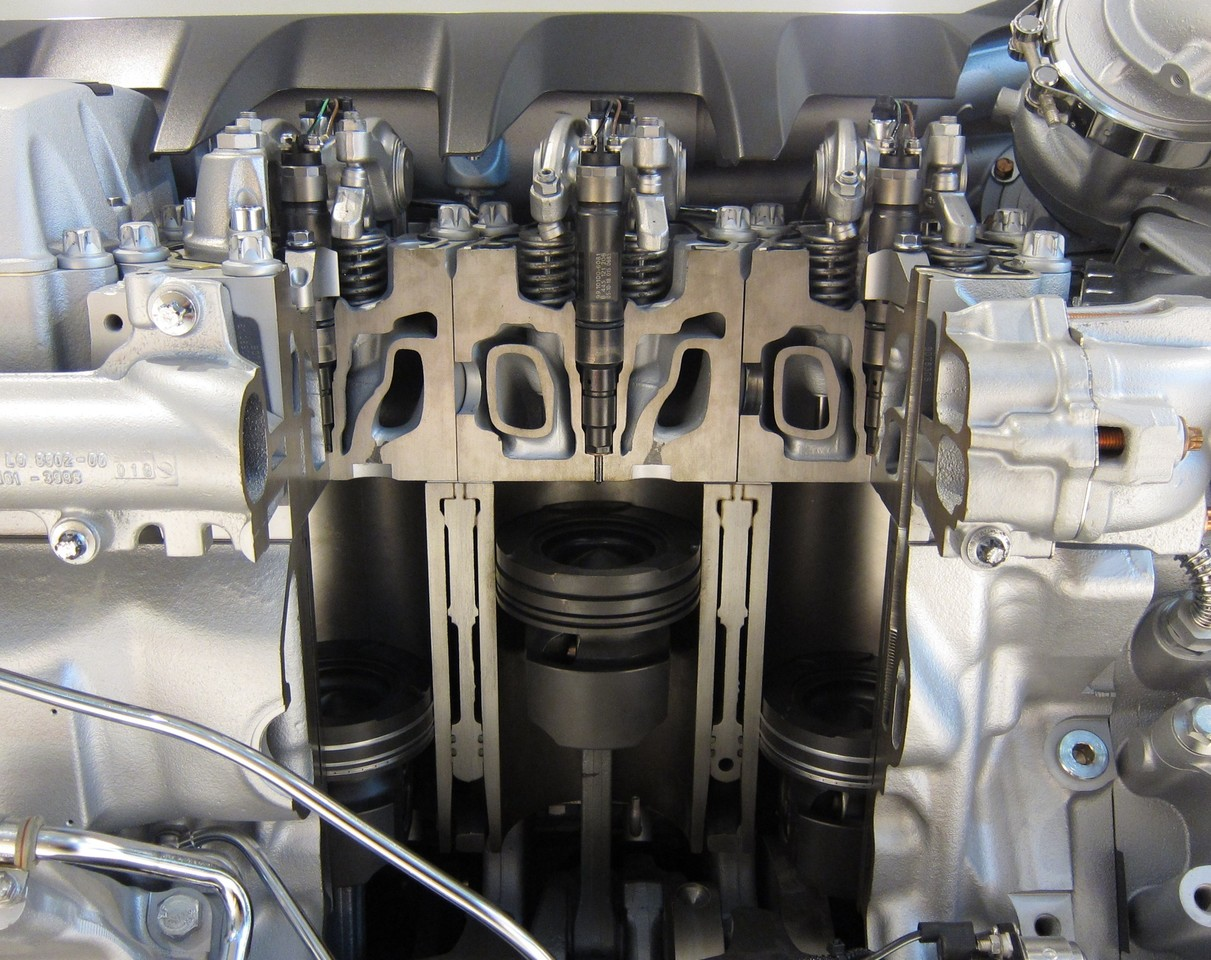
\includegraphics[width=8cm]{images/diesel_engine_cutaway.jpg}
			\end{center}
			\supercaption{Une découpe dans un moteur de camion laisse apparaître trois pistons dans leurs cylindres. Un système fermé est un bon outil pour étudier l’air emprisonné dans un cylindre. Le moteur photographié est un diesel \textsc{man} en V8.}%
				{\wcfile{Cutaway of a MAN V8 Diesel engine.jpg}{Photo} \ccbysa \olivier}
				\label{fig_diesel_engine_cutaway}
		\end{figure}
		
		L’utilisation d’un système fermé est judicieuse pour analyser les machines à mouvement alternatif (moteurs automobiles, pompes et compresseurs et généralement toutes les machines à pistons/cylindres). Ces machines divisent le fluide en petites quantités qui sont emprisonnées dans une enclave, dans laquelle elles sont chauffées, refroidies, comprimées ou détendues (\cref{fig_diesel_engine_cutaway}). Il est alors facile d’identifier une quantité de masse donnée et de quantifier les transferts qu’elle subit.
		
		À l’inverse, pour étudier ce qui se passe dans une tuyère de turboréacteur par exemple, nous aurions des difficultés pour identifier un groupe donné de particules et quantifier le changement de ses propriétés. Il sera alors judicieux d’utiliser un système ouvert, comme nous l’étudierons au \courstrois.
		
		Concrètement, dans ce chapitre, nous voulons quantifier le travail qu’on peut générer avec un fluide dans un cylindre. Un moteur de voiture fournit du travail parce que l’air dans les cylindres fournit plus de travail en se détendant au retour qu’il n’en a reçu à en se faisant comprimer à l’aller (\cref{fig_moteur_sf}). Comment peut-on générer cela ? Pour répondre à cette question, il nous faut une méthode robuste pour quantifier les transferts d’énergie.

		\begin{figure}
			\begin{center}
			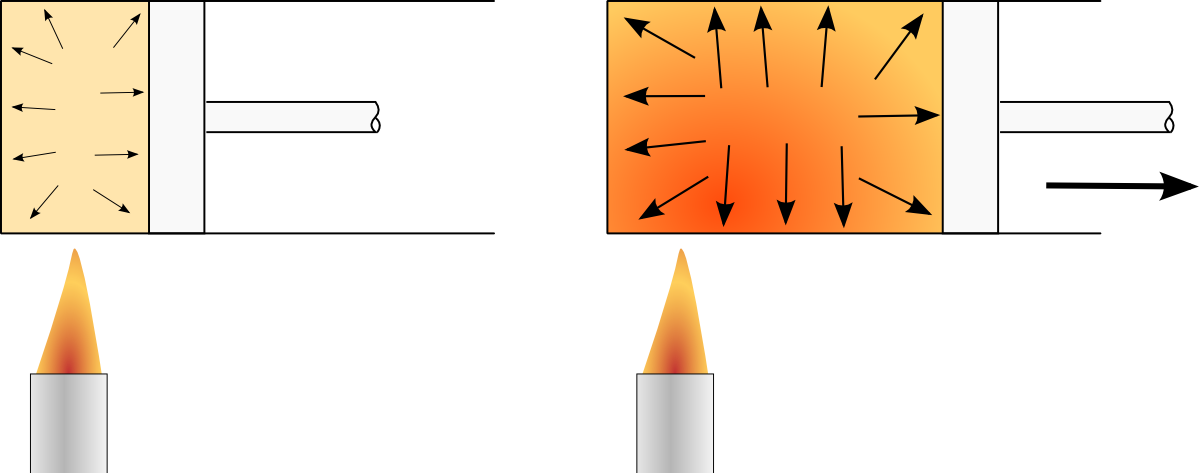
\includegraphics[width=\textwidth]{images/fonctionnement_base_moteur.png}
			\end{center}
			\supercaption{Principe de fonctionnement d’un moteur. Lorsque l’on fournit de la chaleur à un fluide dans un réservoir fermé, celui-ci augmente les forces qu’il exerce sur les parois du réservoir. En laissant le réservoir se déformer, on fait effectuer un travail au fluide.}{schéma \cczero \oc}
			\label{fig_moteur_sf}
		\end{figure}


\section{Conventions de comptabilité}
\label{ch_conventions_compta_sf}

	\subsection{Le système fermé}

			Nous appelons \vocab{système fermé} un sujet d’étude arbitraire dont les frontières sont imperméables à la masse : un ensemble donné de particules, de masse fixe. Toutes les propriétés de cet ensemble (pression, température, volume, etc.) peuvent être amenées à changer, mais il s’agit toujours des mêmes molécules, non mélangées à d’autres. Par exemple, un gaz prisonnier dans un cylindre et comprimé par un piston (\cref{fig_piston_m_cste}) est parfaitement décrit avec un système fermé.

		\begin{figure}
			\begin{center}
			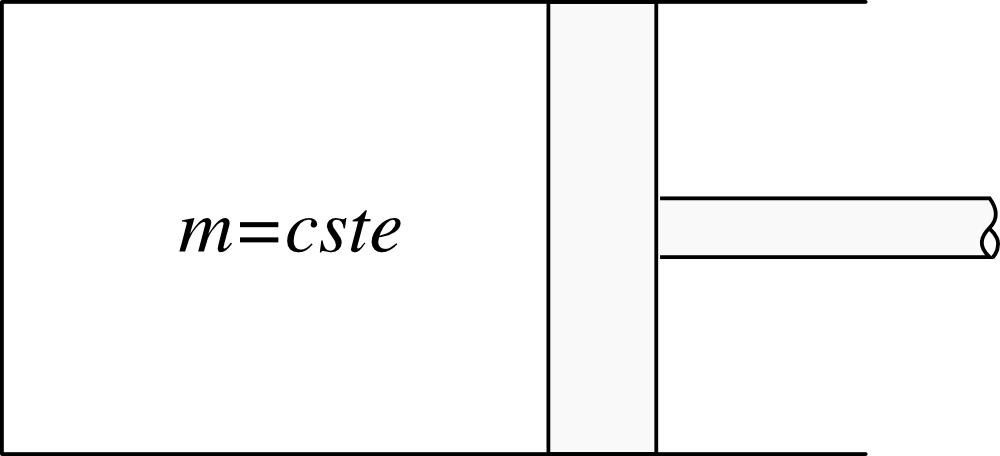
\includegraphics[width=6cm]{images/piston_cylindre.png}
			\end{center}
			\supercaption{Un système fermé typique : une quantité de masse fixe dans un réservoir fermé.
Une paroi mobile permet de la comprimer ; nous lui ferons également recevoir et perdre de la chaleur.}{schéma \cczero \oc}
			\label{fig_piston_m_cste}
		\end{figure}

	\subsection{Conventions de signe}
	\label{ch_convention_signe_sf}

		Pour quantifier les transferts nous utiliserons la convention de signe suivante, illustrée en \cref{fig_convention_signe_sf} :

		\begin{itemize}
			\item Lorsqu’ils sont positifs, les transferts $Q$ et $W$ traduisent une \emph{réception} par le système.
			\item À l’inverse, lorsqu’ils sont négatifs, les transferts $Q$ et $W$ indiquent une \emph{perte} du système. Le travail $W$ est alors fourni et la chaleur $Q$ émise.
		\end{itemize}

		\begin{figure}
			\begin{center}
				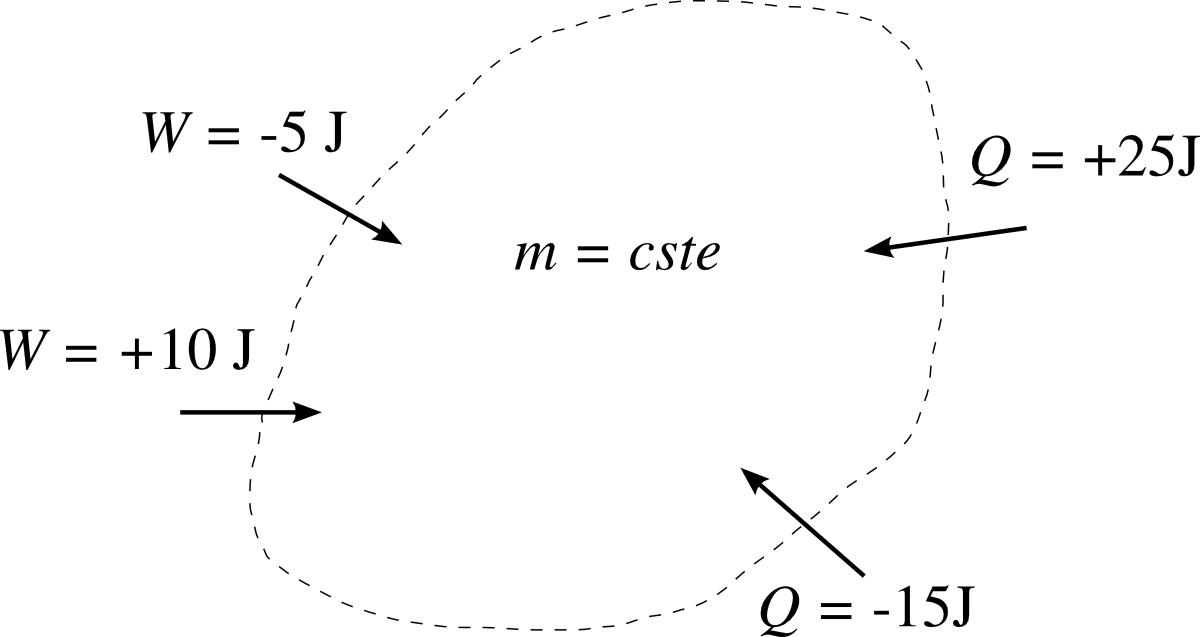
\includegraphics[width=9cm]{images/convention_systeme_ferme.png}
			\end{center}
			\supercaption{Conventions de signe pour un système fermé. Les flux entrants sont positifs, les flux sortants sont négatifs ; ils sont tous représentés avec des flèches rentrantes. La quantité de masse est fixe.}{schéma \cczero \oc}
			\label{fig_convention_signe_sf}
		\end{figure}

		Ainsi, dans les équations, nous pouvons systématiquement additionner les termes sans avoir à connaître le sens des transformations. Les transferts sont comptabilisés comme sur un compte bancaire : les dépenses sont négatives et les recettes positives.



\section{Le premier principe dans un système fermé}
\label{ch_premier_principe_sf}

	\thermoquotebegin{O}
		Appelons ainsi $Q$ la quantité totale de chaleur qui doit être impartie à un corps pendant son passage, d’une manière donnée, depuis une condition à une autre, (toute chaleur prélevée au corps étant comptée comme une quantité négative), alors nous la divisons en trois parties, parmi lesquelles la première est employée à augmenter la chaleur existant véritablement dans le corps, la seconde à produire le travail intérieur et la troisième à produire le travail extérieur. Il va de la seconde partie ce que nous avons déjà dit de la première : qu’elle est indépendante du chemin suivi dans le passage du corps d’un état à un autre, et nous pouvons en conséquence représenter ces deux parties ensemble par une fonction $U$, qui même si nous ne pouvons mieux la définir, nous savons à l’avance au moins être entièrement déterminée par les états initial et final du corps.
	\thermoquoteend{Rudolf Clausius, 1854}{\textit{Über eine veränderte Form des zweiten Hauptsatzes der mechanischen Wärmetheorie~\cite{clausius1854}}\vspace{1em}} %handmade vspace
	Le premier principe stipule que l’énergie est indestructible (\S\ref{ch_premier_principe}). Si on fournit \SI{100}{\joule} de travail à un système fermé et qu’il perd \SI{80}{\joule} sous forme de chaleur, c’est donc que «~son~» énergie a augmenté de~\SI{20}{\joule}. Nous nommons cette variation la \vocab{variation d’énergie interne}, $\Delta U$.
	
	Sous forme d’équation, le premier principe dans un système fermé se traduit par l’équation :
	\begin{equation}
		Q_{1 \to 2} + W_{1 \to 2} = \Delta U
		\label{eq_premier_principe_sf_maj}
	\end{equation}
	\begin{equationterms}
		\item pour un système fermé immobile ;
		\item où \tab $\Delta U = U_2 - U_1$ est la variation d’énergie interne (\si{\joule}),
		\item 	\tab $W_{1 \to 2}$ 	\tab est le travail reçu par le système (\si{\joule}),
		\item et \tab $Q_{1 \to 2}$ 	\tab est la chaleur reçue par le système (\si{\joule}).
	\end{equationterms}

	Malheureusement l’énergie interne $U$ est parfois très difficile à mesurer. Nous verrons dans les chapitres~\quatre et~\cinq que les corps emmagasinent cette énergie interne de différentes façons, et qu’elle est intimement liée à la température. L’énergie interne $U$, par définition, est toujours positive, mais sa variation $\Delta U$ ne l’est pas nécessairement.

	L’\cref{eq_premier_principe_sf_maj} peut être exprimée avec des grandeurs spécifiques :
	\begin{IEEEeqnarray}{rCl}
		m \ ( q_{1 \to 2} + w_{1 \to 2} )		& = & m \ \Delta u \nonumber \\
		q_{1 \to 2} + w_{1 \to 2} 				& = & \Delta u
	\label{eq_premier_principe_sf_min}
	\end{IEEEeqnarray}
	\begin{equationterms}
		\item pour un système fermé immobile ;
		\item où \tab $\Delta u = u_2 - u_1$ est la variation d’énergie interne spécifique (\si{\joule\per\kilogram}),
		\item 	\tab $w_{1 \to 2}$ 	\tab est le travail spécifique reçu par le système (\si{\joule\per\kilogram}),
		\item et \tab $q_{1 \to 2}$ 	\tab\tab est la chaleur spécifique reçue par le système (\si{\joule\per\kilogram}).
	\end{equationterms}
	
	Nous pouvons encore ré-écrire cette \cref{eq_premier_principe_sf_min} pour l’exprimer sous sa \vocab{forme différentielle} :
	\begin{IEEEeqnarray}{rCl}
		\diff q + \diff w	& = & \delta u
	\label{eq_premier_principe_sf_diff}
	\end{IEEEeqnarray}
	\begin{equationterms}
		\item pour un système fermé immobile ;
		\item où \tab $\delta u$ 	\tab\tab est la variation infinitésimale d’énergie interne spécifique (\si{\joule\per\kilogram}),
		\item 	\tab $\diff w$ 	\tab est le transfert infinitésimal de travail spécifique (\si{\joule\per\kilogram}),
		\item et \tab $\diff q$ 	\tab est le transfert infinitésimal de chaleur spécifique (\si{\joule\per\kilogram}).
	\end{equationterms}

	Dans cette \cref{eq_premier_principe_sf_diff}, les opérateurs $\diff$ et $\delta$ ont le même sens mathématique (celui de quantités infinitésimales) mais des significations phyiques différentes : $\diff w$ représente un \emph{transfert} infinitésimal qui s’intégrera en $w_{1 \to 2}$, tandis que $\delta u$ représente une \emph{variation} infinitésimale qui s’intégrera en $\Delta u = u_2 - u_1$.
	
	Lorsqu’un fluide est ramené à son état initial (même pression, même volume, même température), alors il contient exactement la même quantité d’énergie interne qu’auparavant. La totalité de l’énergie qu’il a reçue (sous forme de chaleur ou de travail) a donc nécessairement été rendue à l’extérieur sous une forme ou une autre. Nous exprimons cette affirmation ainsi :
	\begin{equation}
	Q_{\text{cycle}} + W_{\text{cycle}} = 0
	\label{eq_premier_principe_cycle}
	\end{equation}
	\begin{equationterms}
		\item pour un cycle thermodynamique complet,
		\item où \tab $W_{\text{cycle}}$ \tab est le travail reçu par le système (\si{\joule}),
		\item et \tab $Q_{\text{cycle}}$ \tab est la chaleur reçue par le système (\si{\joule}).
	\end{equationterms}

	Cette \cref{eq_premier_principe_cycle} est la raison pour laquelle on énonce souvent le premier principe de la façon suivante, sans pourtant apporter grand’chose à notre simple affirmation du \coursunshort :

	«~Lorsqu’un système a parcouru un cycle thermodynamique complet, la somme algébrique de la chaleur fournie et du travail effectué est nulle.~»



\section{Quantifier le travail avec un système fermé}

	Le calcul du travail avec les fluides est délicat. Nous allons procéder en trois étapes~de complexité croissante :

	\begin{itemize}
		\item En remplaçant le fluide par un ressort ;
		\item En comprimant le fluide de façon infiniment lente ;
		\item En comprimant le fluide de façon rapide.
	\end{itemize}



	\subsection{Le travail en fonction du volume, avec un ressort}
	\label{ch_travail_pdv}

		\begin{figure}
			\begin{center}
				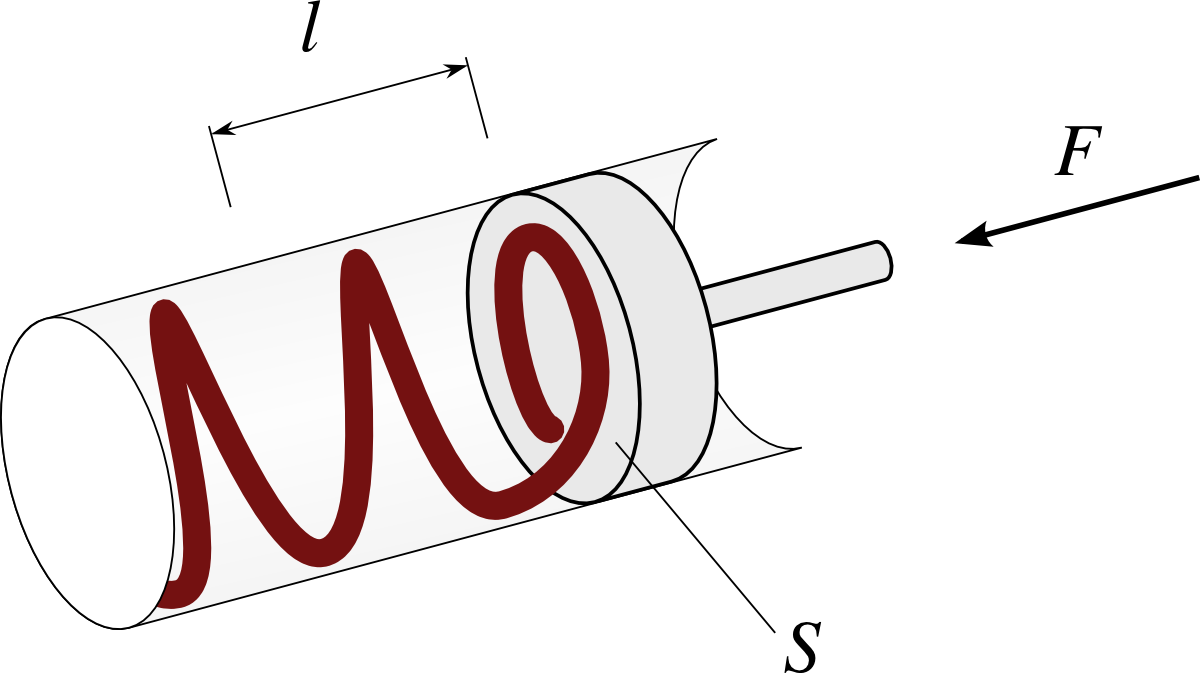
\includegraphics[width=12cm]{images/travail_cylindre_1.png}
			\end{center}
			\supercaption{Dans un premier temps, nous modélisons le fluide à l’intérieur du système avec un ressort métallique.}{schéma \ccbysa \olivier}
			\label{fig_piston_ressort}
		\end{figure}

		Commençons par imaginer que le fluide au sein d’un système fermé se comporte comme un ressort métallique (\cref{fig_piston_ressort}). C’est une modélisation intéressante pour débuter notre étude. Nous avions vu en \S\ref{ch_travail_fdl} que le travail fourni ou reçu par un ressort s’exprimait selon :
		\begin{equation*}
			W_\fromatob = - \int_\A^\B {F \diff l} \tag{\ref{eq_travail_fdl}}
		\end{equation*}

		Aujourd’hui, comme nous utilisons un fluide, nous voulons exprimer le travail en fonction des propriétés \vocab{pression} et \vocab{volume} plutôt que force et longueur.

		\clearfloats
		\begin{description}

			\item[La pression]{se définit comme une force divisée par une aire :
			\begin{equation}
				p \equiv \frac{F}{S}
				\label{def_pression}
			\end{equation}
			\begin{equationterms}
				\item où \tab $p$ \tab est la pression (\si{\pascal}),
				\item 	\tab $F$ \tab est la force (\si{\newton}),
				\item et \tab $S$ \tab est l’aire de la surface sur laquelle la force s’applique (\si{\metre\squared}).
			\end{equationterms}

			L’unité \textsc{si} de la pression est le~\si{Pascal},
			\begin{equation}
				\SI{1}{\pascal} \equiv \SI{1}{\newton\per\metre\squared}
			\end{equation}
			mais il est usuel d’utiliser le~\si{bar} pour unité :
			\begin{equation}
			\SI{1}{bar} \equiv \SI{1e5}{\pascal}
			\end{equation}

			Notons que la pression atmosphérique à faible altitude est de l’ordre du bar ($p_{\text{atm.std.}} \equiv \SI{1}{atm} \equiv \SI{1,01325}{bar}$). Attention, les manomètres indiquent parfois une pression jaugée, qui n’est pas la pression réelle. Cette différence est décrite dans l’annexe \ref{ch_annexe_pression}.
			}% end item

			\item[Le volume]{est également exprimable facilement. Si le système est déformé par un piston d’aire $S$, de sorte que sa longueur varie de $\diff l$, nous avons :
			\begin{equation}
			\diff V = S \diff l
			\label{eq_volume_surface_longueur}
			\end{equation}
			\begin{equationterms}
				\item où \tab $\diff V$ 	\tab est la variation infinitésimale du volume (\si{\metre\cubed}),
				\item 	\tab $S$ 			\tab\tab l’aire du piston déplacé (\si{\metre\squared}),
				\item et \tab $\diff l$ 	\tab\tab la variation infinitésimale de longueur du système correspondant au déplacement du piston (\si{\metre}).
			\end{equationterms}

			Dans le système d’unités \textsc{si} le volume se mesure en~\si{\metre\cubed} mais l’unité de mesure la plus courante est le~\si{litre} ($\SI{1}{\liter} \equiv \SI{e-3}{\metre\cubed})$.
			}% end item
		
		\end{description}


		Exprimons maintenant le travail d’un système fermé en fonction du volume et de la pression. En insérant les équations~\ref{def_pression} et~\ref{eq_volume_surface_longueur} dans l’\cref{eq_travail_fdl} nous obtenons :
		\begin{IEEEeqnarray}{rCl}
			W_\fromatob 	& = & - \int_\A^\B {F \diff l} = - \int_\A^\B {\frac{F}{S} S \diff l} 	\nonumber \\
			W_\fromatob 	& = & - \int_\A^\B {p \diff V} \label{eq_travail_pdV}
		\end{IEEEeqnarray}
		\begin{equationterms}
			\item pour un système fermé modélisé par un ressort,
			\item où \tab $W_\fromatob$ 	est le travail reçu par le système (\si{\joule}),
			\item 	\tab $p$ 				\tab\tab est la pression (homogène) intérieure (\si{\pascal}),
			\item et \tab $\diff V$ 		\tab la variation du volume (\si{\metre\cubed}).
		\end{equationterms}

		Pour pouvoir quantifier l’énergie stockée ou fournie par le système, il nous suffira donc de connaître la relation entre $p$ et $V$. Dans le cas présent, cette fonction $p_{(V)}$ est directement liée à la caractéristique $F_{(l)}$ du ressort. La dureté du ressort et sa géométrie (à spires régulières ou progressives) détermineront au final la quantité de travail stockée et fournie par le système.
		
		Un outil absolument formidable pour comprendre et analyser les transferts de chaleur est le \vocab{diagramme pression-volume}. Dans le cas où l’on modélise le fluide par un ressort, le travail peut être visualisé par l’aire sous la courbe d’une évolution (\cref{fig_p-v_ressort}).		

		\begin{figure}
			\begin{center}
				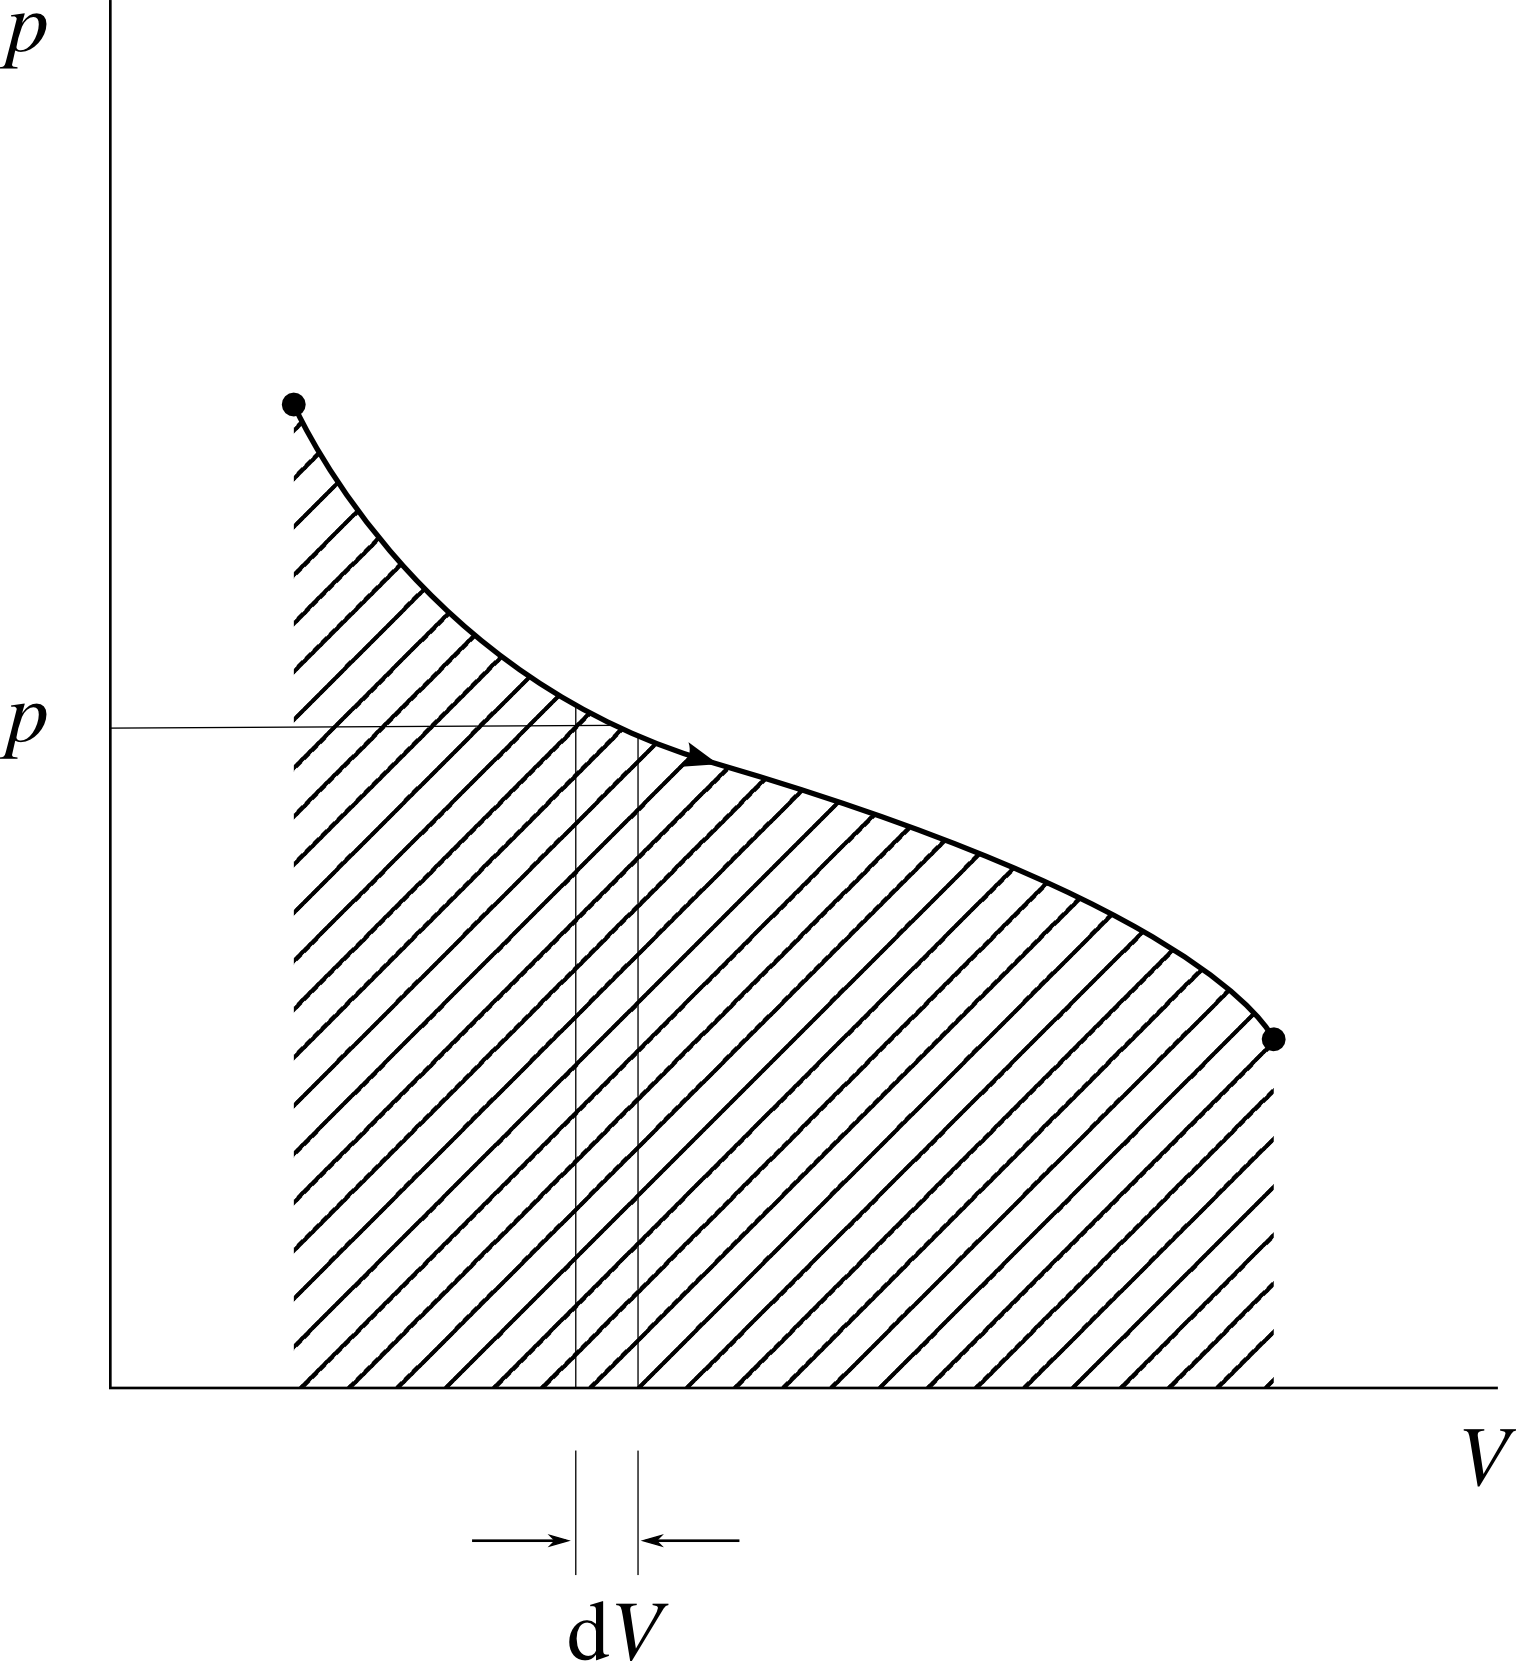
\includegraphics[width=8cm]{images/pv_ressort.png}
			\end{center}
			\supercaption{Diagramme pression-volume d’un système fermé modélisé par un ressort. Dans le cas représenté, le volume augmente (le piston s’éloigne). La grandeur $\diff V$ sera constamment positive, et le travail sera négatif : le système perd de l’énergie au profit du piston.\\
			Cette figure représente le même phénomène qu’en \cref{fig_force-déplacement-aire} avec des grandeurs différentes.}{}
			\label{fig_p-v_ressort}
		\end{figure}

		\begin{anexample}
			
			Un système fermé est constitué d’une boîte vide dans laquelle on a placé un ressort. La pression exercée par le ressort sur les parois de la boîte est constante à $p = \SI{e5}{\pascal}$ quelque soit son volume. On comprime la boîte depuis un volume $V_\A = \SI{2}{\liter}$ jusqu’à $V_\B = \SI{1}{\liter}$. Quel est le transfert de travail ?
				\begin{answer}
						Sur un diagramme pression-volume et de façon qualitative (c’est-à-dire sans représenter les valeurs numériques), l’évolution peut être représentée ainsi :
							\begin{center}
								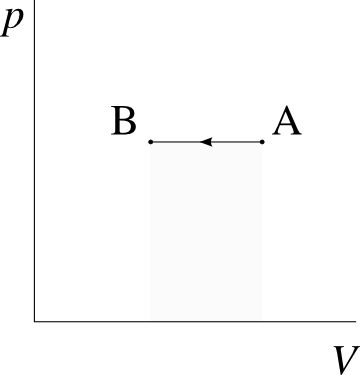
\includegraphics[width=3cm]{images/exe_pv_isobare.png}
							\end{center}
					Nous partons de l’équation \ref{eq_travail_pdV} : $W_{\A\to\B} = - \int_\A^\B p \diff V = - p_\text{cste.} \int_\A^\B \diff V = p_\text{cste.} \left[V\right]_{V_\A}^{V_\B } = - \num{e5} (\num{1e-3} - \num{2e-3}) = \SI{+100}{\joule}.$
					\begin{remark}Le signe est positif : la boîte («~le système~») reçoit du travail. Nous explicitons toujours le signe en quantifiant les transferts.\end{remark}
				\end{answer}
		\end{anexample}


		\begin{anexample}
			Un système fermé a une pression interne liée à son volume par la relation $p = \num{7e5} - \num{2e8} \ V$ (en unités \textsc{si}). On comprime la boîte depuis un volume $V_\A = \SI{2}{\liter}$ jusqu’à $V_\B = \SI{1}{\liter}$. Combien a-t-il reçu ou perdu d’énergie sous forme de travail ?
				\begin{answer}
						Sur un diagramme pression-volume et de façon qualitative, l’évolution peut être représentée ainsi :
							\begin{center}
								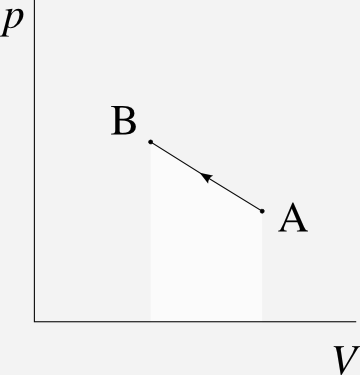
\includegraphics[width=3cm]{images/exe_pv_prop.png}
							\end{center}
					Encore une fois nous partons de l’\cref{eq_travail_pdV} : $W_{\A\to\B} = - \int_\A^\B p \diff V = - \int_\A^\B (\num{7e5} - \num{2e8} V) \diff V = - \left[\num{7e5}V - \frac{1}{2}\num{2e8} V^2\right]_{V_\A}^{V_\B } = - (\num{700} - 100 - \num{1400} + 400) = \SI{+400}{\joule}$ (positif : travail reçu par le système).
				\end{answer}
		\end{anexample}
		

	\subsection{Travail d’un fluide en évolution lente}

		Lorsque l’on comprime un fluide, les molécules qui le composent sont plus rapprochées les unes des autres (\cref{fig_molécules_compression_lente}) et les collisions entre elles et contre les parois deviennent plus fréquentes. À l’échelle macroscopique, cette augmentation se traduit par une augmentation de la pression.
		
		\begin{figure}
			\begin{center}
			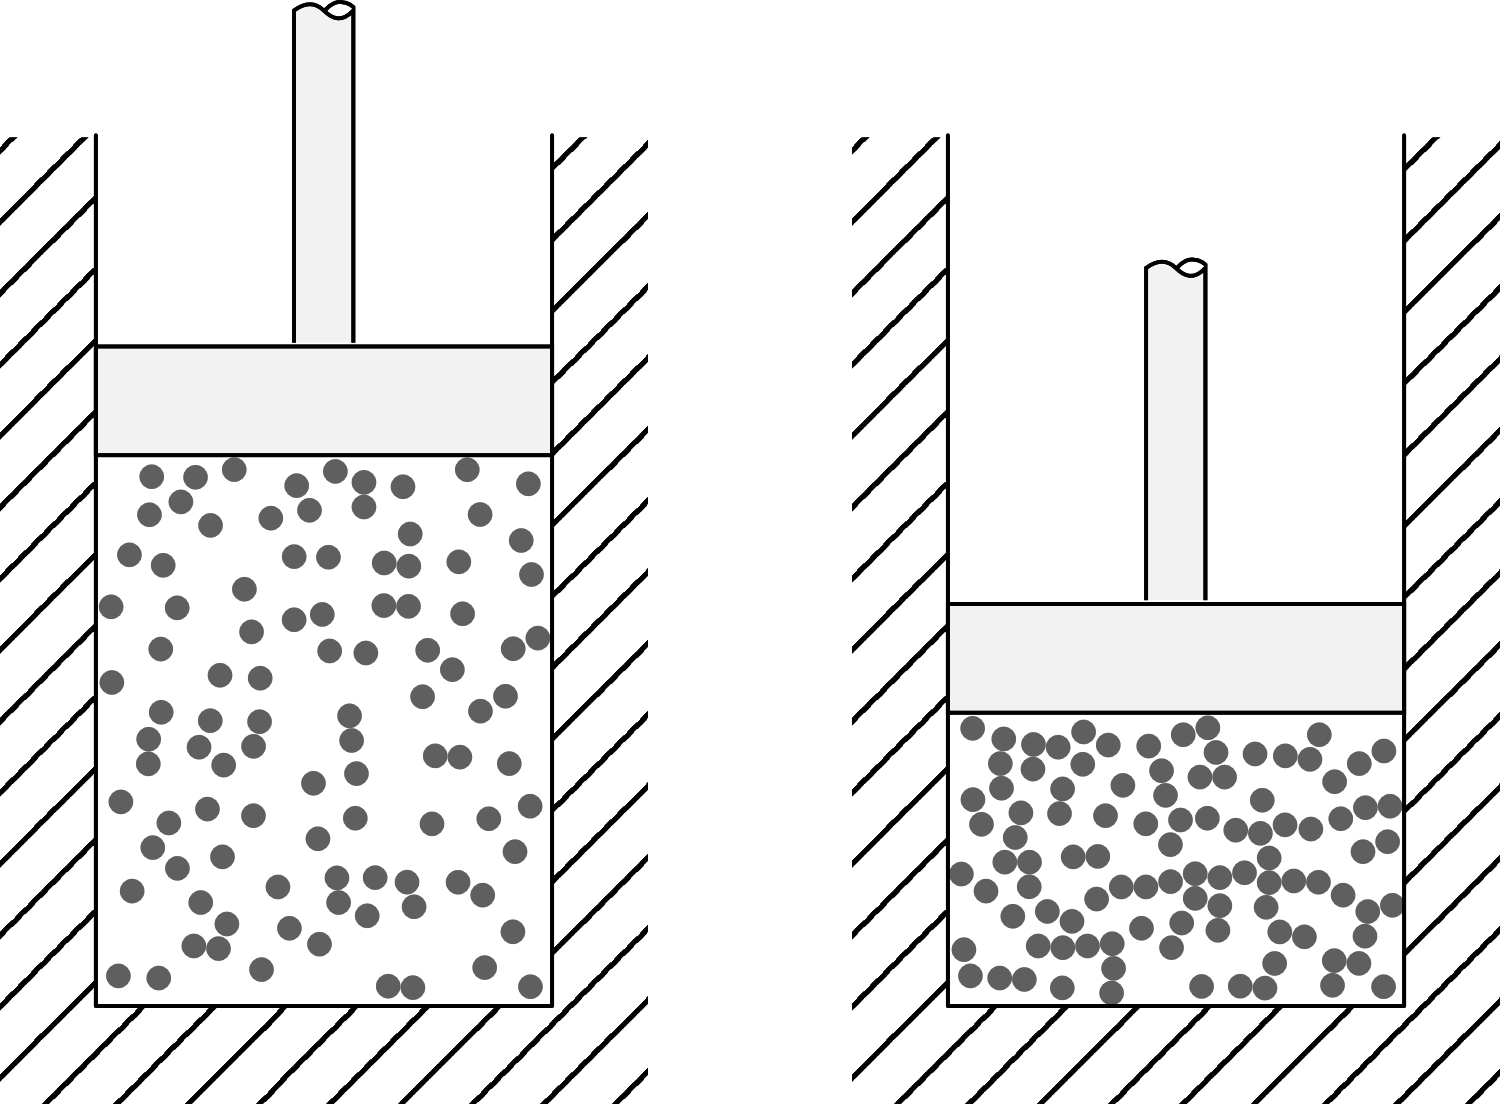
\includegraphics[width=9cm]{images/particules_compression_lente.png}
			\end{center}
			\supercaption{Une représentation simpliste d’un fluide que l’on \mbox{comprime} infiniment lentement sans le chauffer. Le fluide voit sa température et sa pression augmenter.}{schéma \cczero \oc}
			\label{fig_molécules_compression_lente}
		\end{figure}

		Nous constatons expérimentalement que lorsque le mouvement est infiniment lent, un fluide comprimé se comporte exactement comme un ressort (\cref{fig_piston_fluide_lent}). La précision «~lorsque le mouvement est infiniment lent~» est d’importance capitale, comme nous le verrons plus bas.

		\begin{figure}
			\begin{center}
			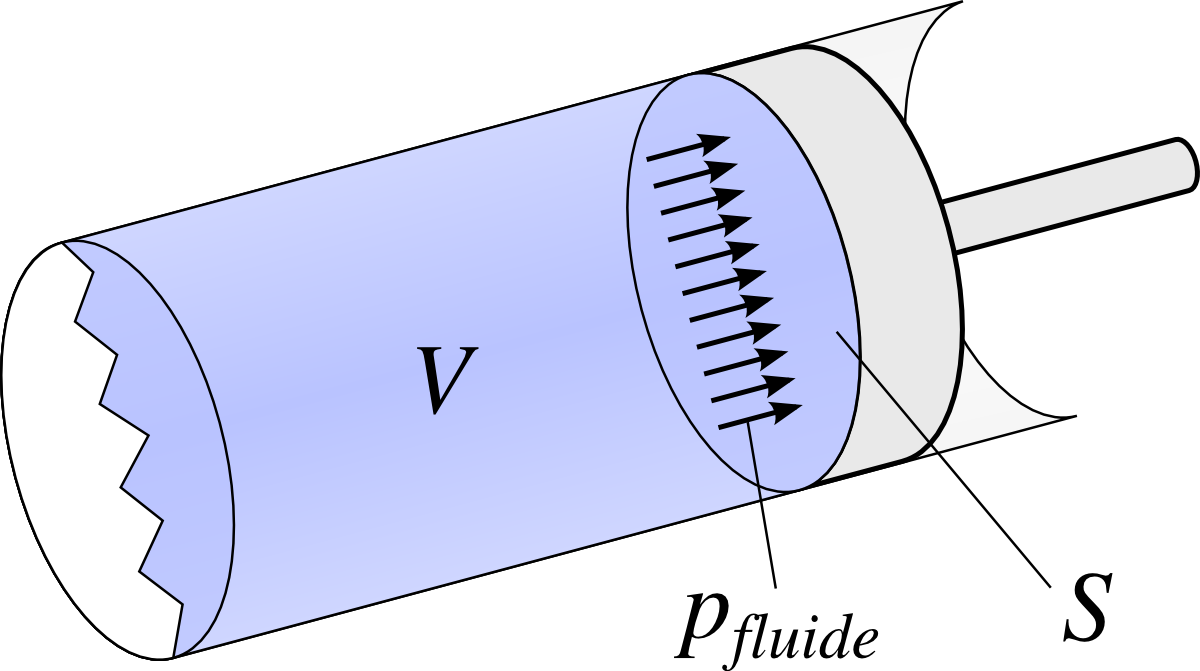
\includegraphics[width=10cm]{images/travail_cylindre_2.png}
			\end{center}
			\supercaption{Lorsque le mouvement du piston est infiniment lent, le fluide se comporte comme un ressort que l’on comprime.}{schéma \ccbysa \olivier}
			\label{fig_piston_fluide_lent}
		\end{figure}

		
		Si cette condition est respectée, nous pouvons exprimer le travail reçu ou perdu par le système de la même façon qu’avec le ressort de la section précédente :		
		\begin{IEEEeqnarray}{rCl}
			W_\fromatob 	& = & - \int_\A^\B {p \diff V}	\nonumber \\
			w_\fromatob 	& = & - \int_\A^\B p \diff v
			\label{eq_travail_pdv}
		\end{IEEEeqnarray}
		\begin{equationterms}
			\item pour un système fermé lorsque les variations de volume sont infiniment lentes ;
			\item où \tab $w_\fromatob$ 	\tab est le travail spécifique reçu par le système (\si{\joule\per\kilogram}),
			\item 	\tab $p$ 				\tab\tab est la pression (homogène) intérieure (\si{\pascal}),
			\item et \onlyamphibook{\tab} $\diff v $ 		\onlyamphibook{\tab} la variation du volume spécifique (\si{\metre\cubed\per\kilogram}). % floating quote messes with the tabs in Framabook, so they are commented out here.
		\end{equationterms}
		
		\thermoquotebegin{O}
			Cela posé, prenons un gaz quelconque à la température $T$ […]; représentons son volume $v_o$ par l’abscisse \textsc{ab}, et sa pression par l’ordonnée \textsc{cb}.[…] Le gaz, pendant sa dilatation, aura développé une quantité d’action mécanique qui aura pour valeur l’intégrale du produit de la pression, par la différentielle du volume, et qui sera représentée géométriquement par la surface comprise entre l’axe des abscisses, les deux coordonnées \textsc{cb}, \textsc{de}, et de la portion d’hyperbole~\textsc{ce}.
		\thermoquoteend{Benoît Paul Émile Clapeyron, 1834\\ {\tiny(le premier diagramme $p-v$…)}}{\textit{Mémoire sur la puissance motrice de~la~chaleur}~\cite{clapeyron1834}\vspace{6em}} %handmade vspace
		Sur un graphique représentant la pression en fonction du volume spécifique, ce travail $w_\fromatob$ est représenté par la surface sous la courbe de A à B, exactement comme la \cref{fig_p-v_ressort}. La forme de la courbe, c’est-à-dire la relation entre $p$ et $v$ au fur et à mesure de l’évolution, déterminera la quantité $w_\fromatob$ .

		\begin{figure}
			\begin{center}
			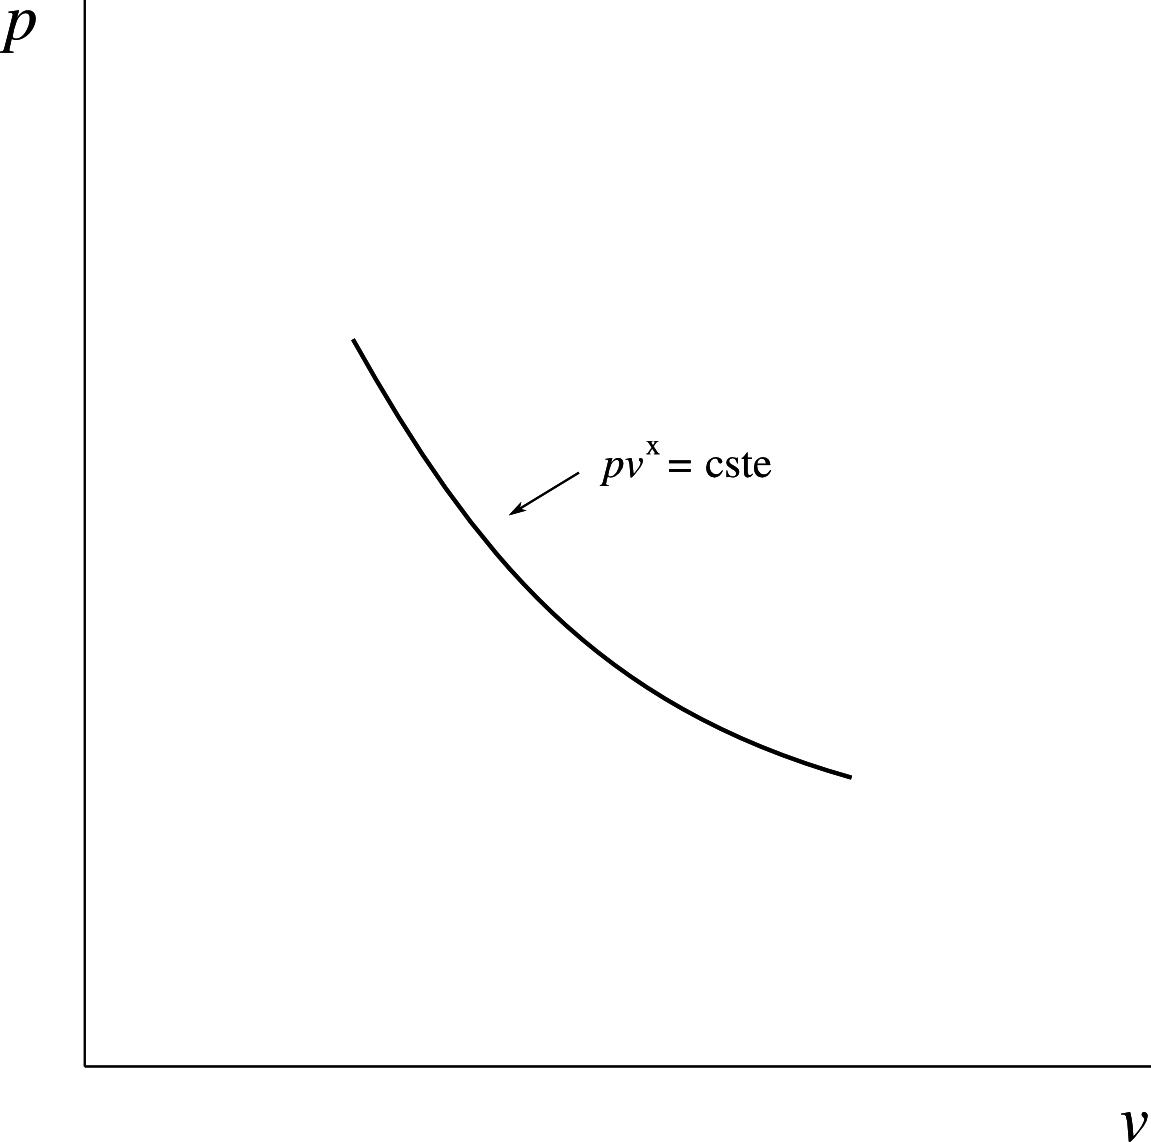
\includegraphics[width=\pvdiagramwidth]{images/pv_gaz_simple.png}
			\end{center}
			\supercaption{Propriétés d’un gaz lorsqu’on le comprime. La relation est similaire à celle que l’on obtiendrait avec un ressort à spires progressives.}{schéma \cczero \oc}
			\label{fig_p-v_pvx}
		\end{figure}

		\thermoquotebegin{O}
			S’il était vrai que la vapeur se dépensât par le cylindre à une pression égale à celle de la chaudière, ou qui fût à celle-ci dans un rapport fixe indiqué par un coefficient quelconque, puisqu’il faut toujours à une même locomotive le même nombre de tours de roue, ou le même nombre de coups de piston pour parcourir la même distance, il s’en suivrait que tant que ces machines travaillent à la même pression, elles devraient consommer dans tous les cas la même quantité d’eau pour la même distance.
		\thermoquoteend{François-Marie Guyonneau de~Pambour, 1839}{\textit{Théorie de la machine à vapeur} \cite{pambour1839}\vspace{4em}} %handmade vspace
		Comment les fluides se comportent-t-ils lorsqu’on les comprime --\ autrement dit, par quel type de «~ressort~» peut-on les modéliser ? On constate expérimentalement que, lorsqu’on les comprime, la plupart des gaz voient leur pression et leur volume liés par une relation de type $p\ v^{x} = \text{cste.}$ avec $x$ une constante lorsqu’on les comprime (\cref{fig_p-v_pvx})%
			\footnote{Toutefois, nous verrons au \courscinqshort que les liquides/vapeurs ne se comportent pas du tout comme cela sur une plage de propriétés donnée, même si la tendance globale reste la même.}%
		.

		Lorsqu’on apporte de la chaleur au fluide pendant qu’on le comprime, on «~durcit~» son comportement, et la pression augmente plus rapidement (\cref{fig_p-v_ajout_retrait_chaleur}). À~l’inverse, lorsqu’on lui prélève de la chaleur pendant la compression, la pression augmente moins rapidement. Ces transferts de chaleur font donc varier la quantité de travail à fournir pour comprimer le fluide entre deux volumes donnés.
		
		Le cas où l’on apporte pas de chaleur est nommé \vocab{adiabatique} : $Q = 0$. Attention : adiabatique ne veut pas dire «~à température constante~». Lorsque l’on comprime un fluide sans apport de chaleur, sa température augmente. Dans un moteur diesel, par exemple, l’air dans les cylindres peut atteindre \SI{900}{\degreeCelsius} avant la combustion -- ce qui est désirable, comme nous le verrons au \courssept.

		\begin{figure}
			\begin{center}
			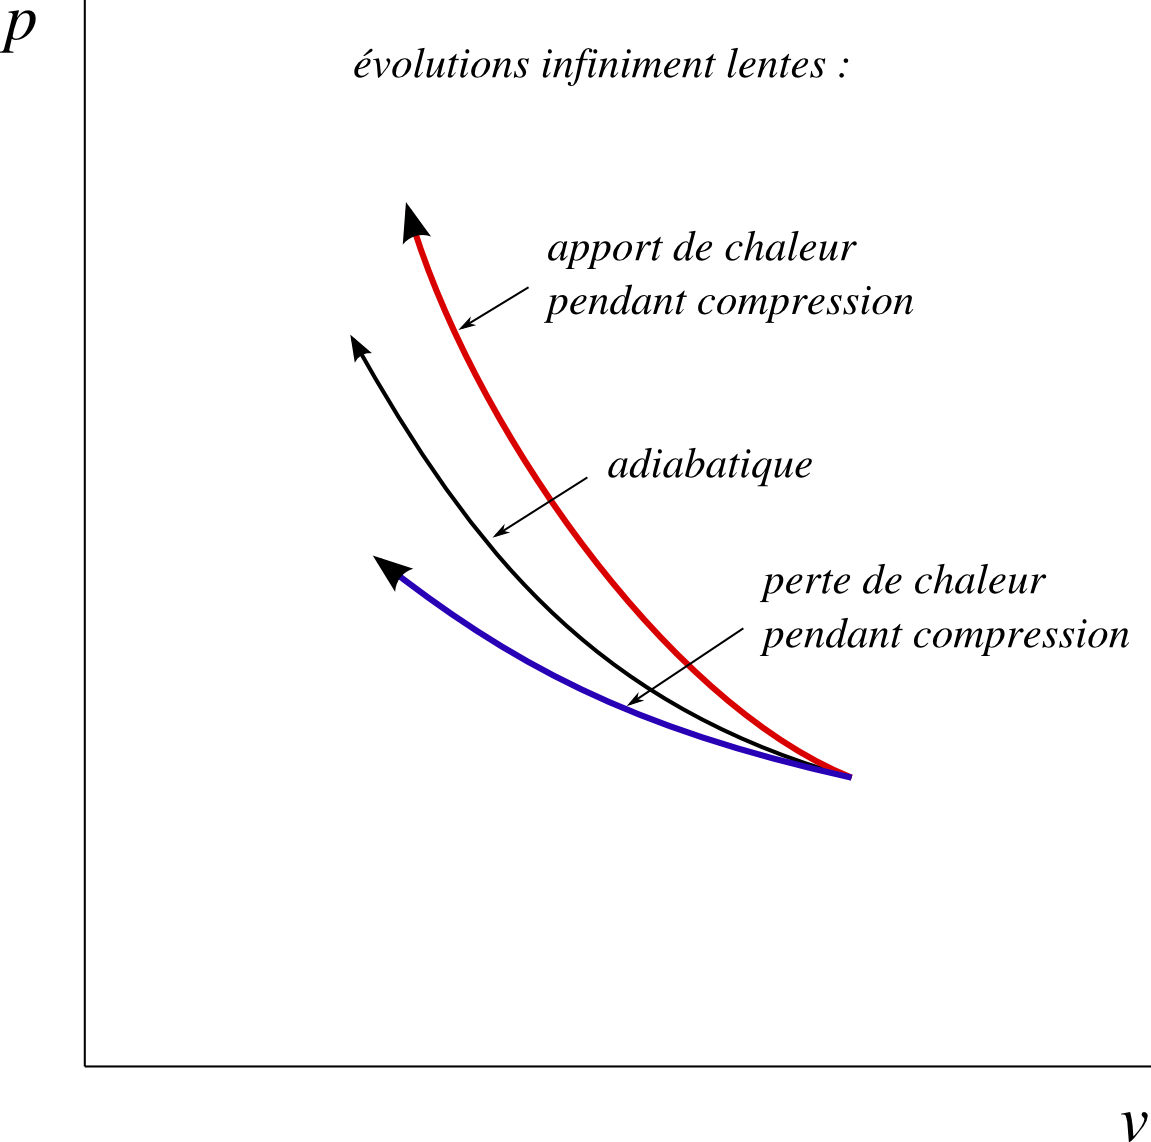
\includegraphics[width=\didacticpvdiagramwidth]{images/pv_transfert_chaleur.png}
			\end{center}
			\supercaption{Comportement d’un fluide lorsqu’on le comprime infiniment lentement.
Plus on lui apporte de chaleur pendant la compression, plus la pression augmente fortement. La courbe adiabatique représente le cas où aucun apport ni perte de chaleur n’a lieu ($Q = 0$).}{schéma \cczero \oc}
			\label{fig_p-v_ajout_retrait_chaleur}
		\end{figure}


		Dans les trois évolutions de la \cref{fig_p-v_ajout_retrait_chaleur}, la relation de type $p v^{x} = \text{cste.}$ reste une modélisation appropriée. Plus on apporte de chaleur pendant la compression, plus la pression augmente rapidement --\ l’exposant $x$ est alors plus important.

		Inversement, si l’on prélève de la chaleur pendant la compression, la pression augmente moins rapidement et on obtient une courbe plus proche de l’horizontale (avec un exposant $x$ plus faible). En prélevant suffisamment de chaleur, on peut même maintenir la pression constante, comme nous le verrons aux chapitres~\quatre et~\cinq. L’exposant $x$ est alors nul et on a $p = p_\text{cste.}$.
		
			\begin{anexample}
				Un gaz dans un cylindre est comprimé lentement par un piston. On observe que sa pression est liée à son volume par la relation $p v^{\num{1,2}} = k$ (en unités \textsc{si}, et où $k$ est une constante). Au début de la compression, ses propriétés sont $p_\A = \SI{1}{\bar}$ et $v_\A = \SI{1}{\metre\cubed\per\kilogram}$. On le comprime jusqu’à ce que son volume ait atteint $v_\B = \SI{0,167}{\metre\cubed\per\kilogram}$. \\
				Quelle quantité de travail spécifique le gaz a-t-il fourni ou reçu ?				
					\begin{answer}
						Sur un diagramme pression-volume et de façon qualitative, l’évolution peut être représentée ainsi :
							\begin{center}
								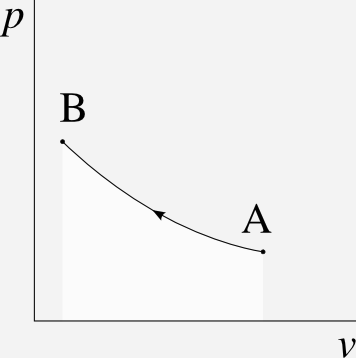
\includegraphics[width=3cm]{images/exe_pv_exp1.png}
							\end{center}
						Il nous faut d’abord calculer la valeur de $k$ pour connaître quantitativement la relation entre $p$ et $v$. Nous l’obtenons avec les conditions initiales : $k = p_\A v_\A^{\num{1,2}} = \num{e5} \times 1^{\num{1,2}} = \SI{e5}{\usi}$.
							\begin{remark} La grandeur de $k$ est déroutante : elle est mesurée en~\si{\pascal\metre\tothe{3,6}\per\kilogram\tothe{1,2}}. Cela n’a pas d’importance pour nous et il nous suffit (après avoir bien converti les unités d’entrée en \textsc{si}!) d’indiquer «~unités \textsc{si}~», ou~\si{\usi}.\end{remark}
						Maintenant, nous pouvons décrire $p$ en fonction de $v$ : $p = \num{e5} \times v^{\num{-1,2}}$. Il n’y a plus qu’à intégrer en partant de l’\cref{eq_travail_pdv} : $w_\fromatob = - \int_\A^\B p \diff v = - \int_\A^\B k v^{\num{-1,2}} \diff v = - k \left[\frac{1}{-1,2 + 1} v^{-1,2 - 1} \right]_{v_\A}^{v_\B } = \frac{\num{e5}}{0,2}\left[v^{-0,2}\right]_1^{\num{0,167}} = \SI{+2,152e5}{\joule\per\kilogram} = \SI{+215,2}{\kilo\joule\per\kilogram}$.
							\begin{remark}Le signe est positif : le gaz reçoit du travail.\end{remark}
							\begin{remark}Le résultat peut paraître grand, mais il faut se rappeler que c’est un travail spécifique (\S\ref{ch_valeurs_spécifiques}) qu’il faudra multiplier par la masse du gaz pour obtenir une quantité en joules. Aux conditions de départ (\SI{1}{\kilogram\per\metre\cubed}) un volume d’air de~\SI{1}{\liter} pèse à peine plus d’un~\si{gramme}. \end{remark}
					\end{answer}
			\end{anexample}

			\begin{anexample}
				Une masse de~\SI{0,3}{gramme} de gaz pressurisée dans un cylindre est détendue lentement en laissant un piston se déplacer. On sait que sa pression et son volume sont reliés par une relation de type $p v^{k_1} = k_2$ (où $k_1$ et $k_2$ sont deux constantes).\\
				Au début de la détente, la pression est à~\SI{12}{\bar} et le volume est de~\SI{0,25}{\liter}. Une fois détendu, le gaz arrive à pression ambiante de~\SI{1}{\bar} avec un volume de~\SI{1,76}{\liter}.\\
				Quel travail le gaz a-t-il dégagé pendant la détente ?				
					\begin{answer}
						Sur un diagramme pression-volume et de façon qualitative, l’évolution peut être représentée ainsi :
							\begin{center}
								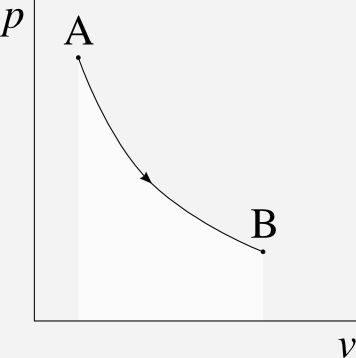
\includegraphics[width=3cm]{images/exe_pv_exp2.png}
							\end{center}
						Il nous faut d’abord connaître entièrement la loi reliant $p$ à $v$ ; ensuite nous procéderons à l’intégration $-\int p \diff v$ pendant l’évolution pour calculer le travail.\\
						Commençons par calculer les volumes spécifiques au départ et à l’arrivée : $v_\A = \frac{V_\A}{m} = \frac{\num{0,25e-3}}{\num{3e-4}} = \SI{0,833}{\metre\cubed\per\kilogram}$. De même, $v_\B = \frac{V_\B }{m} = \SI{5,867}{\metre\cubed\per\kilogram}$.
						Maintenant, nous pouvons calculer $k_1$ :		
							\begin{IEEEeqnarray*}{rCl}
								p_\A v_\A^{k_1} 	&=& p_\B v_\B ^{k_1}	\\
								\left(\frac{v_\A}{v_\B }\right)^{k_1} &=& \frac{p_\B }{p_\A}\\
								k_1 \ln\left(\frac{v_\A}{v_\B }\right) &=& \ln \left(\frac{p_\B }{p_\A}\right)\\
								k_1 &=& \frac{\ln\left(\frac{p_\B }{p_\A}\right)}{\ln\left(\frac{v_\A}{v_\B }\right)} = \frac{\ln\left(\frac{1}{12}\right)}{\ln\left(\frac{0,833}{5,867}\right)} = \num{1,2733}
							\end{IEEEeqnarray*}
						Et avec $k_1$, nous pouvons calculer $k_2 = p_\A v_\A^{k_1} = \num{12e5} \times \num{0,833}^{\num{1,2733}} = \SI{9,514e5}{\usi}$.
							\begin{remark}$k_1$ est un exposant et n’a pas d’unités. Les unités de $k_2$ ne nous intéressent pas.\end{remark}
							\begin{remark}Même si elle peut paraître laborieuse, cette démarche «~nous avons un modèle général pour la tendance, quels sont les paramètres pour ce cas particulier ?~» est très courante en physique, et extrêmement utile pour l’ingénieur/e.\end{remark}
						Nous savons maintenant décrire quantitativement les propriétés pendant l’évolution : $p v^{\num{1,2733}} = \num{5,914e5}$.	Il n’y a plus qu’à effectuer notre intégration habituelle : $w_\fromatob = - \int_\A^\B p \diff v = - k_2 \int_\A^\B v^{-k_1} \diff v = \frac{\num{-9,514e5}}{\num{-0,2733}} \left[v^{-0,2733}\right]_{\num{0,833}}^{\num{0,587}} = \SI{-3,333e6}{\joule\per\kilogram} = \SI{-3333}{\kilo\joule\per\kilogram}$. Nous multiplions par la masse de gaz pour obtenir le travail : $W_{\A\to\B} = m \ w_\fromatob = \SI{-1}{\kilo\joule}$.
							\begin{remark}Ce calcul peut être effectué de façon plus rapide, sans calculer les valeurs de $v_\A$, $v_\B $ et $k_2$. Toutefois, pour être certain/e de parvenir au résultat, il est plus sûr et plus facile de quantifier $p$ et $v$ (en \textsc{si}) à tous les stades de l’évolution avant de débuter une intégration.\end{remark}
					\end{answer}
			\end{anexample}
			
			\begin{anexample}
				Un gaz enfermé dans un réservoir hermétique est chauffé lentement. Son volume reste bloqué à~\SI{12}{\liter}, et sa pression évolue de~\SI{1}{\bar} jusqu’à \SI{40}{\bar}. Quel est le travail développé ?
					\begin{answer}
						Sur un diagramme pression-volume et de façon qualitative, l’évolution peut être représentée ainsi :
							\begin{center}
								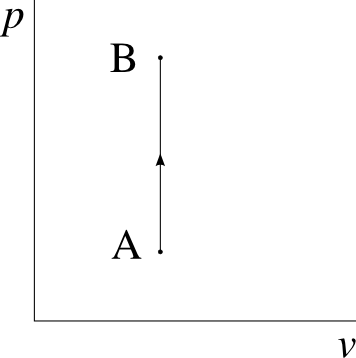
\includegraphics[width=3cm]{images/exe_pv_isochore.png}
							\end{center}
						Le travail est nul, bien sûr. Le volume ne changeant pas, $\diff V$ est nul pendant toute l’évolution. Nous pouvons chauffer ou refroidir à loisir, mais tant qu’aucune paroi n’est déplacée, il n’y aura pas de transfert de travail.
					\end{answer}
			\end{anexample}
			

	\subsection{Travail d’un fluide en évolution rapide}
	\label{ch_évolutions_irr_sf}

		\thermoquotebegin{O}
			Nous avons dit qu’à l’origine du mouvement l’équilibre de pression s’établit entre la chaudière et le cylindre, mais à mesure que la vitesse du piston s’accroît, celui-ci fuit en quelque sorte devant la vapeur sans lui donner le temps d’établir cet équilibre, et la pression dans le cylindre baisse \mbox{nécessairement}.
		\thermoquoteend{François-Marie Guyonneau de~Pambour, 1835}{\textit{Traité théorique et pratique des machines locomotives}~\cite{pambour1835}\vspace{3em}} %handmade vspace
		Les choses se compliquent lorsque nous comprimons et détendons notre fluide de façon rapide (\cref{fig_molécules_rapide}). Il se produit alors un phénomène complexe et d’importance critique en thermodynamique : \textbf{la pression sur la paroi est différente de la «~pression moyenne~» à l’intérieur du fluide}.

		\begin{figure}
			\begin{center}
			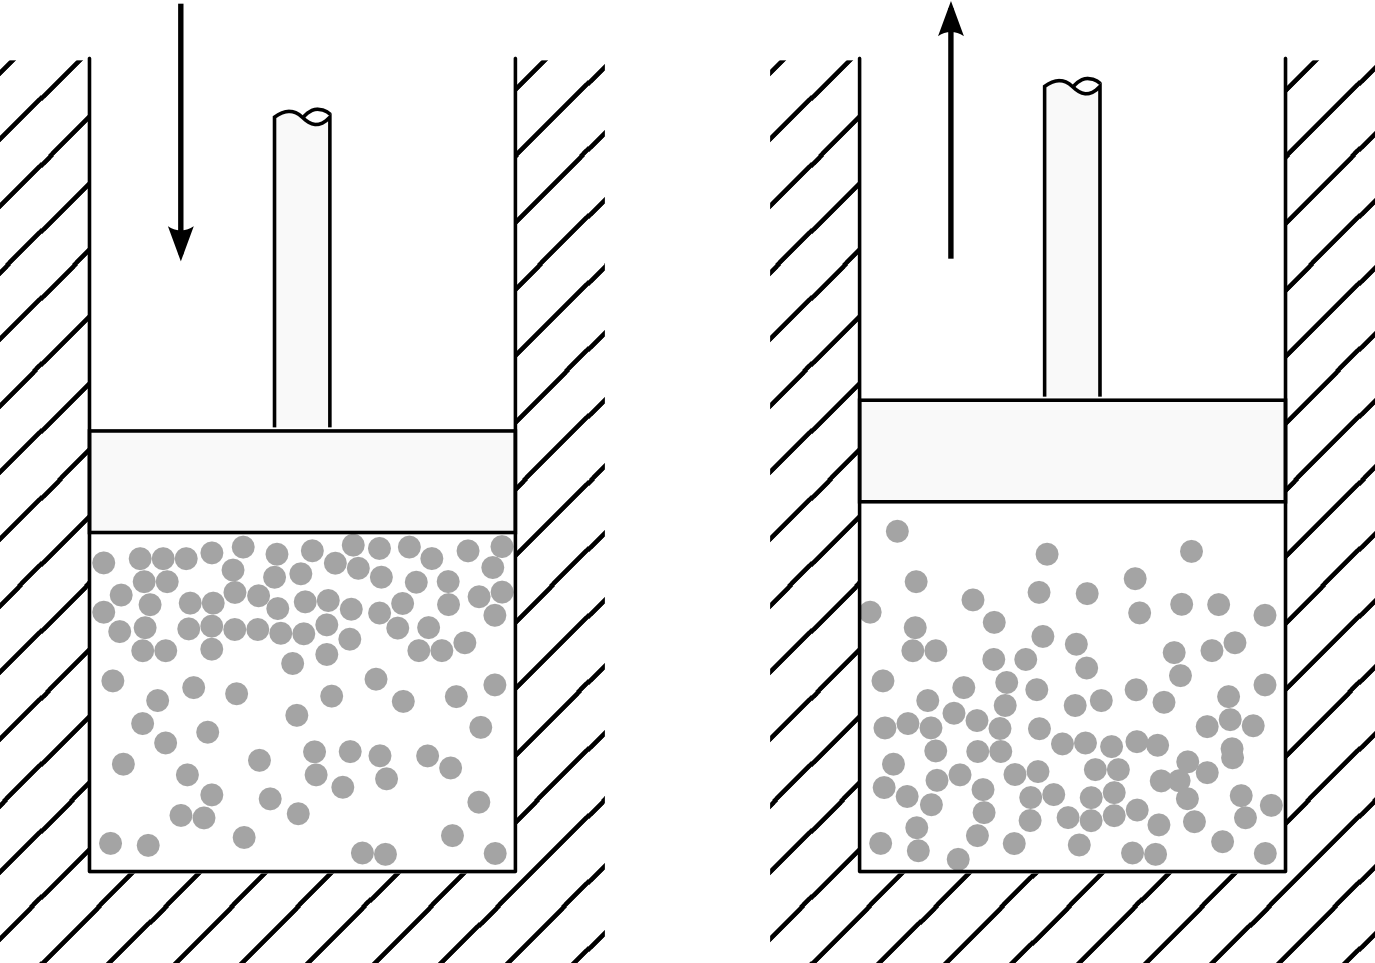
\includegraphics[width=9cm]{images/particules_compression_rapide.png}
			\end{center}
			\supercaption{Compression et détente irréversibles. Lorsqu’on comprime un fluide de façon brutale (schéma de gauche), la pression sur la paroi du piston est augmentée. Lors d’une détente brutale (schéma de droite) cette pression est diminuée.}{schéma \ccbysa \olivier}
			\label{fig_molécules_rapide}
		\end{figure}

		Pour décrire ce qui se passe à l’intérieur du fluide, nous pouvons prendre l’exemple de l’eau d’une baignoire que l’on pousse avec les mains --\ comme la paroi mobile dans le réservoir représenté en \cref{fig_baignoire}. Lorsque le piston est éloigné et rapproché brutalement, la pression sur ses parois n’est pas la même que lorsqu’il est déplacé lentement.

		\begin{figure}[htb!]%handmade: Là il faut poser les figures avant de continuer, sinon ça devient trop dur à suivre.
			\begin{center}
				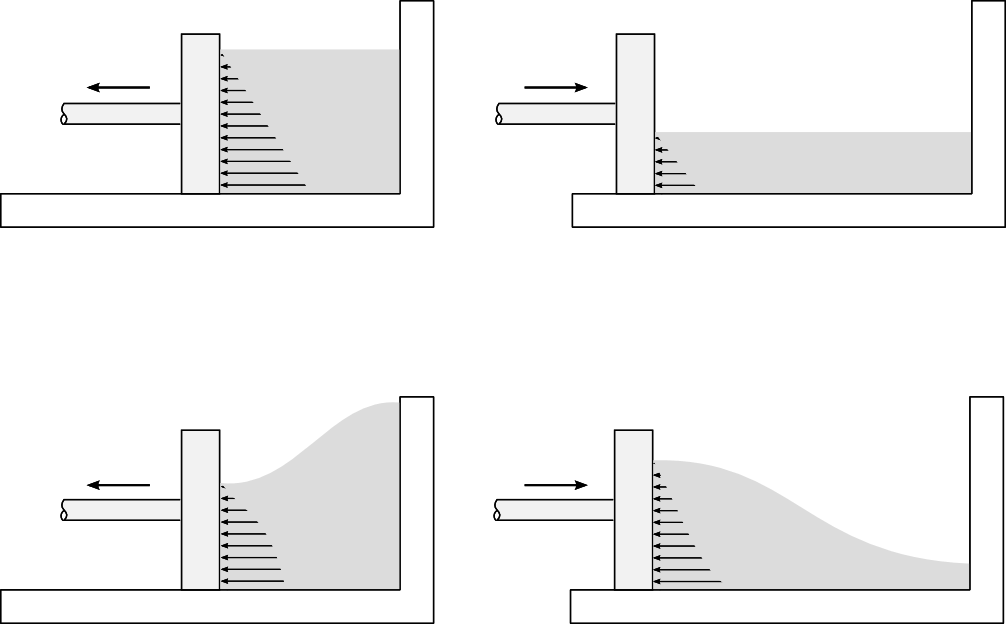
\includegraphics[width=\textwidth]{images/mouvement_rapide_niveau_eau.png}
			\end{center}
			\supercaption{Paroi mobile déplaçant une masse d’eau dans un réservoir : en haut, selon un mouvement infiniment lent ; en bas, avec un mouvement brutal. Les flèches représentent la pression appliquée sur la paroi mobile par l’eau.}{schéma \cczero \oc}%FIXME : vérifier seuil d’originalité, cette figure est repiquée de Çengel & al 2007
			\label{fig_baignoire}
		\end{figure}
		
		Dans chacun des cas, la quantité de travail consommé à la compression est plus grande et la quantité de travail fourni à la détente est plus petite.
		
		Nous nommons ce phénomène l’\vocab{irréversibilité}. Elle nous sera d’un grand embarras dans notre étude quantitative de la thermodynamique et elle rendra encore plus ardues nos conversions de travail et chaleur.

		Que se passe-t-il donc dans le cylindre empli de fluide, lorsqu’on ne le comprime pas de façon infiniment lente ? Lors d’une compression brutale, la pression sur la paroi du piston est plus grande que la pression moyenne à l’intérieur du cylindre (\cref{fig_piston_fluide_rapide}). On dépense \emph{plus d’énergie que nécessaire} pour effectuer le déplacement.

		\begin{figure}
			\begin{center}
				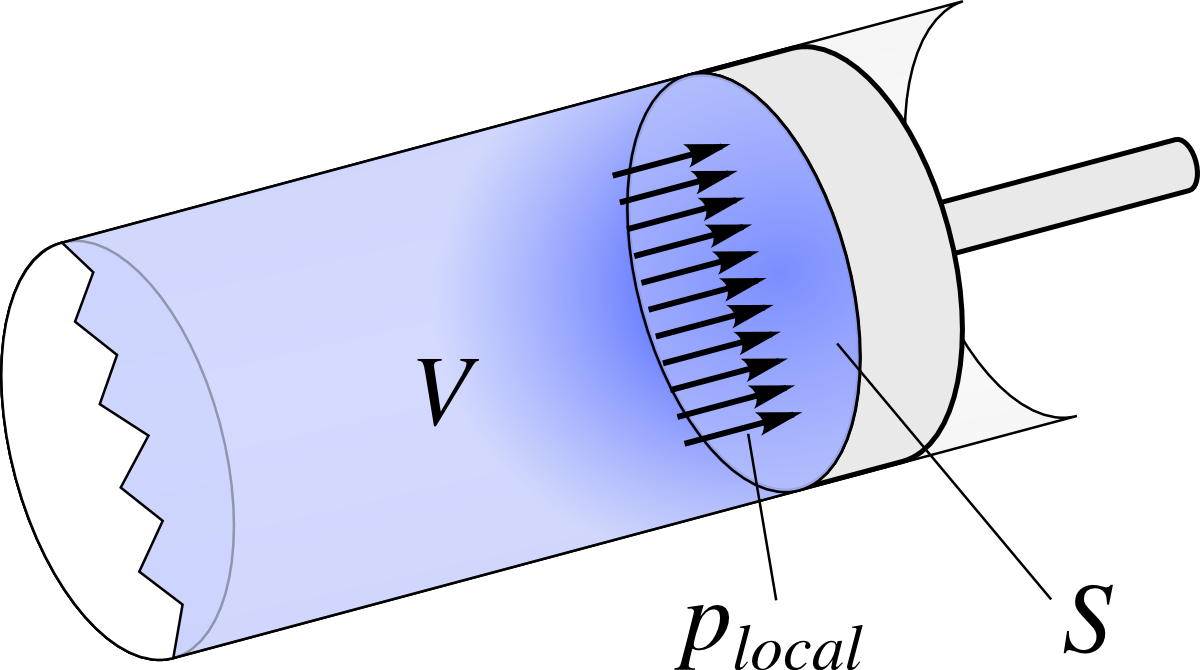
\includegraphics[width=10cm]{images/travail_cylindre_3.png}
			\end{center}
			\supercaption{Fluide comprimé de façon brutale. La pression locale à la surface du piston est supérieure à ce qu’elle aurait été avec un mouvement lent.}{schéma \ccbysa \olivier}
			\label{fig_piston_fluide_rapide}
		\end{figure}

		On pourrait ainsi dire que lorsqu’on le comprime et détend brutalement, un fluide se comporte comme un ressort «~fragile~», à l’intérieur duquel quelque chose se modifie : il n’est pas capable de rendre toute l’énergie mécanique qu’il a emmagasinée.

		Si le travail reçu n’est pas égal au travail restitué, alors où est passé l’excédent d’énergie ? Ce surcroît d’énergie, fourni sous forme de travail par le piston, est \emph{transformé en chaleur à l’intérieur du fluide} pendant les mouvements.

		\clearfloats % encore une fois, sinon c’est trop b****lique

		L’évolution tracée sur un diagramme pression-volume (\cref{fig_p-v_compression_irr}) est bien plus complexe que dans le cas d’une évolution infiniment lente. La pression moyenne à l’intérieur du fluide augmente plus rapidement qu’elle ne le ferait en mouvement lent.

		\begin{figure}
			\begin{center}
				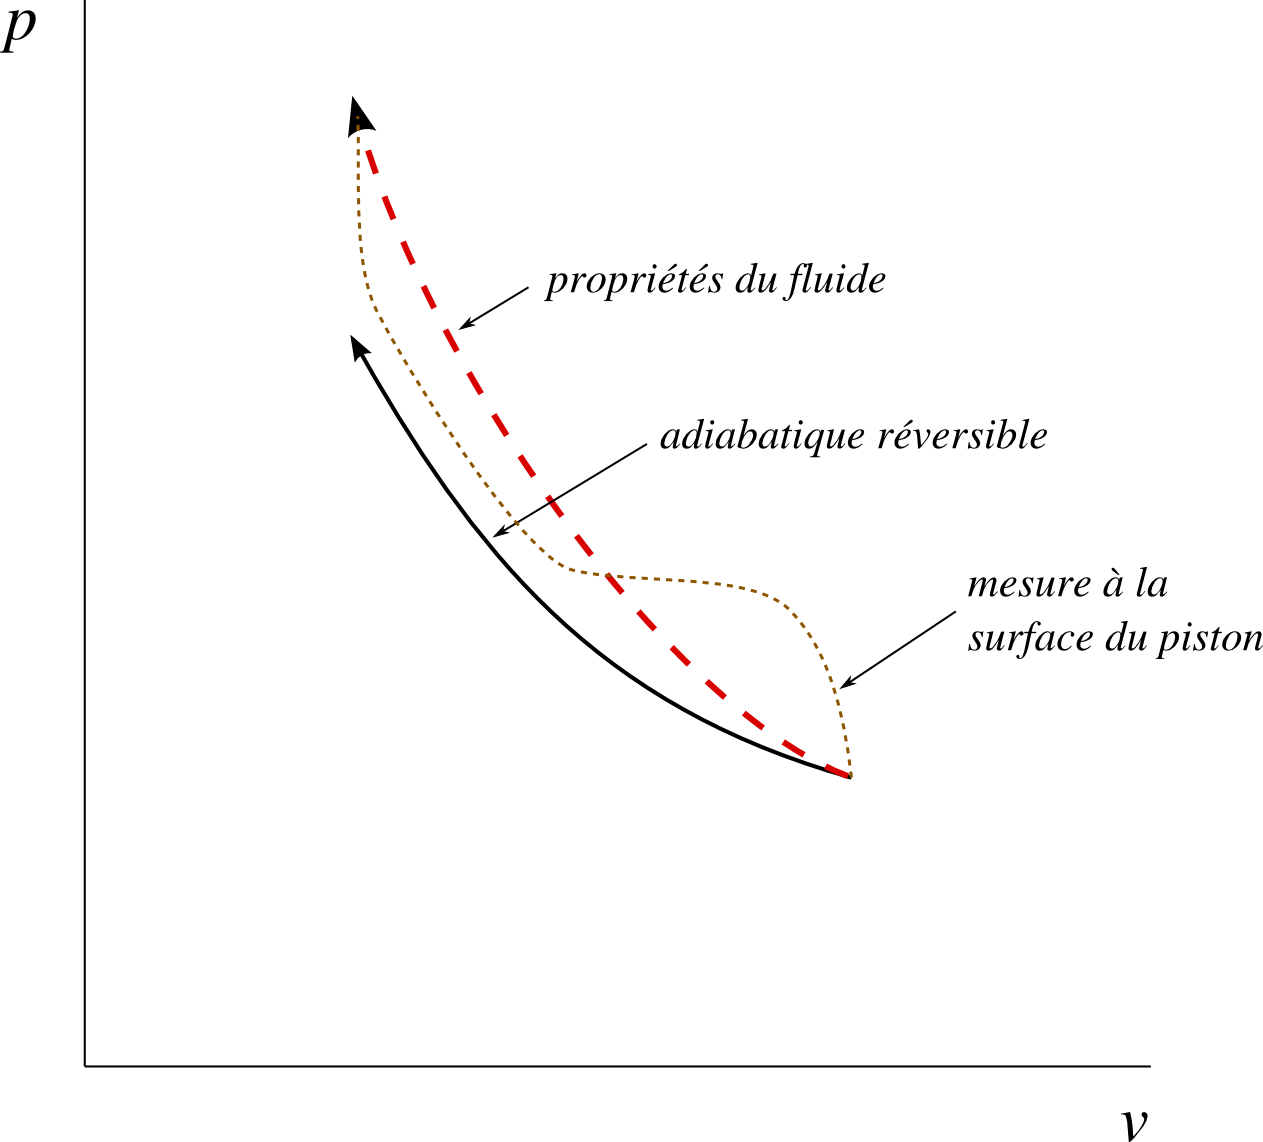
\includegraphics[width=\didacticpvdiagramwidth]{images/pv_compression_irreversible.png}
			\end{center}
			\supercaption{Compression irréversible adiabatique sur un diagramme pression-volume.\\
				Nous représentons l’évolution du gaz en pointillés : il ne s’agit pas d’une série d’états continue car la pression du fluide n’est pas homogène pendant le trajet.\\
				Le chemin qu’aurait suivi le fluide si la compression avait été infiniment lente est représenté avec un trait continu.\\
				Pendant la compression, le «~surcoût~» de travail fourni par le piston est transformé en chaleur (bien que le gaz soit parfaitement isolé).}{schéma \cczero \oc}
			\label{fig_p-v_compression_irr}
		\end{figure}

		Pendant la détente, le phénomène inverse se produit (\cref{fig_p-v_détente_irr}) : une zone de plus faible pression se forme au devant de la paroi du piston, et le travail fourni par le fluide au piston est plus faible qu’il ne l’aurait été dans le cas réversible.

		\begin{figure}
			\begin{center}
			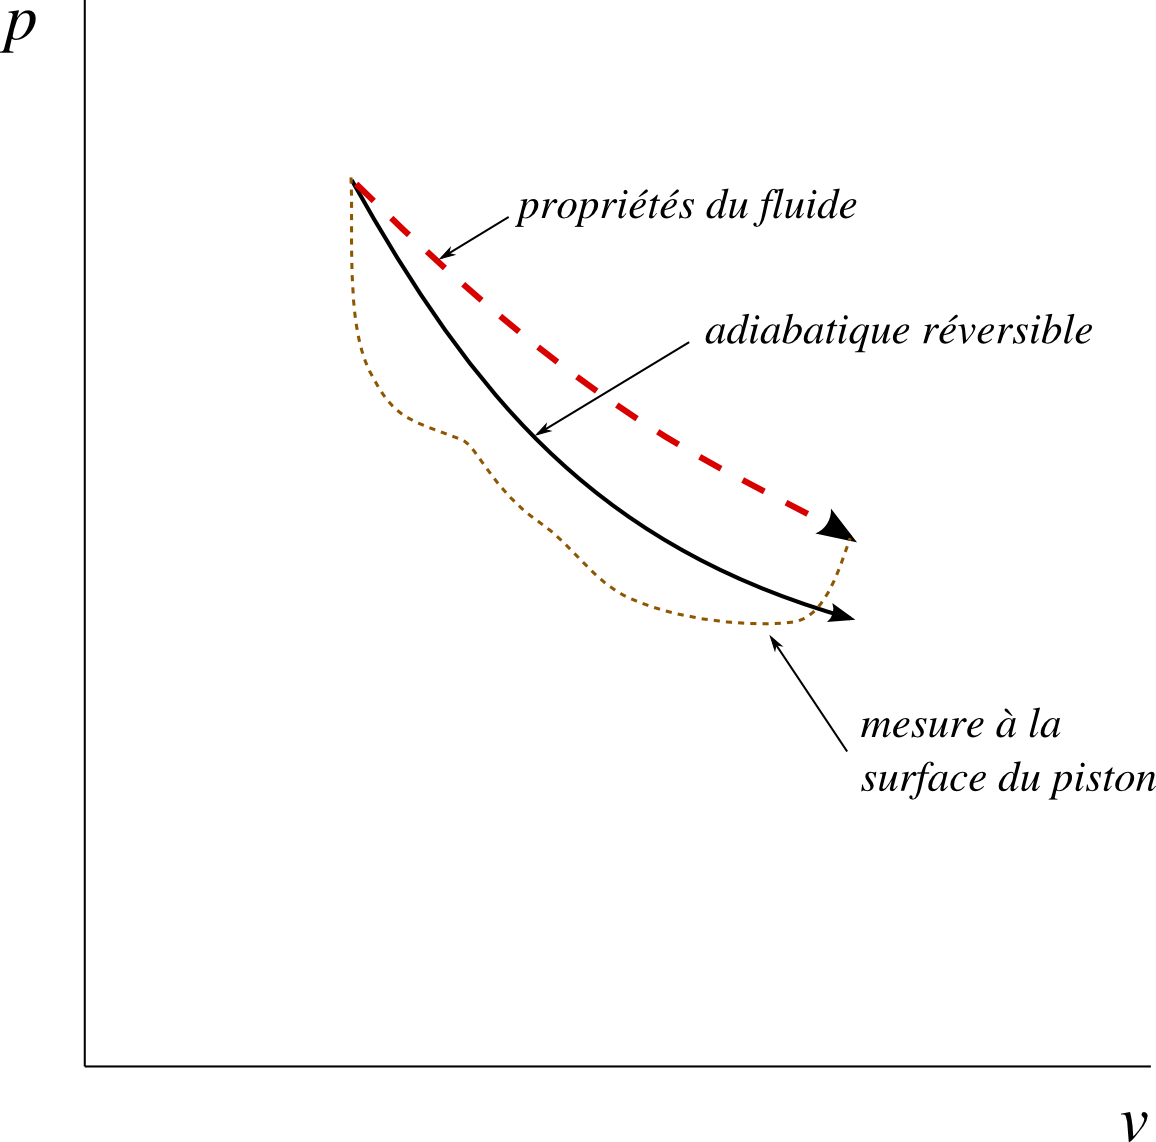
\includegraphics[width=9cm]{images/pv_detente_irreversible.png}
			\end{center}
			\supercaption{Détente irréversible adiabatique sur un diagramme pression-volume.\\ Le travail reçu par le piston est plus faible qu’il ne l’aurait été avec un mouvement lent. Le trajet suivi par le fluide est représenté en pointillés (la pression n’étant pas homogène pendant le mouvement).}{}
			\label{fig_p-v_détente_irr}
		\end{figure}

		D’un point de vue quantitatif, plus les mouvements sur le fluide seront brutaux, et plus l’évolution du fluide ressemblera à une évolution avec apport de chaleur («~durcissement~» du fluide et augmentation de l’exposant $x$ pendant les compressions, diminution de l’exposant $x$ pendant les détentes).

		Par contre, le travail fourni ou reçu par le fluide ne peut plus être simplement calculé par intégrale puisque la pression à l’intérieur du cylindre n’est pas du tout homogène. C’est la pression à la surface du piston qui permettrait de calculer ce travail. Malheureusement, aucune relation mathématique simple ne permet de décrire cette relation entre pression et volume. Il faut effectuer une mesure expérimentale à chaque fois.
		
			
			\begin{anexample}
				On enferme un gaz dans un cylindre hermétique et on effectue des allers-retours entre deux volumes donnés avec le piston, sans transférer de chaleur. Au départ, les allers-retours sont très lents. Ensuite, on effectue les allers-retours de façon très rapide.
				
				Quelle sera l’allure des évolutions sur un diagramme pression-volume ?
					\begin{answer}
						Lors des évolutions lentes, la pression passe toujours par les mêmes valeurs pendant les allers-retours :
							\begin{center}
								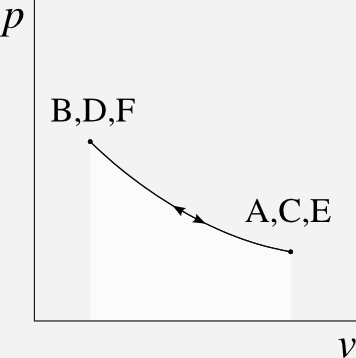
\includegraphics[width=3cm]{images/exe_pv_rev.png}
							\end{center}
						En revanche, pendant les évolutions rapides, à chaque trajet la pression finale est plus grande que ce qu’elle aurait été pendant un trajet lent :
							\begin{center}
								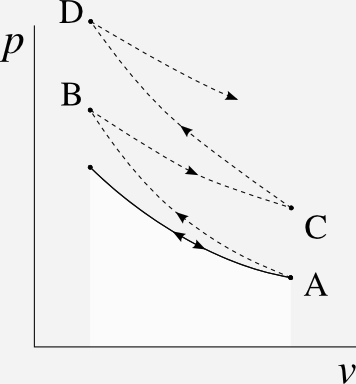
\includegraphics[width=3cm]{images/exe_pv_irr.png}
							\end{center}
						Ainsi, les propriétés s’élèvement progressivement sur le diagramme pression-volume : l’excédent de travail investi pendant les compressions, et le défaut de travail récupéré pendant la détente, se traduisent par une augmentation de l’énergie interne du gaz, dont la température augmente continuellement.
					\end{answer}
			\end{anexample}


	\subsection{La réversibilité}
	\label{ch_reversibilite}
	
		Prenons quelques instants pour réfléchir sur ce que nous venons de décrire. À chaque fois que nous comprimons un fluide «~trop vite~», il se passe quelque chose qui nous empêche de récupérer notre travail.
		
		Du point de vue de l’ingénieur/e, une évolution lente est un cas limite : celui où les dissipations sont minimisées. Par exemple, le travail qu’il faut investir pour comprimer un gaz jusqu’à~\SI{10}{\bar} est minimal lorsque la compression est réversible. De même, une turbine dans laquelle la détente est réversible extraira le maximum de travail d’un fluide comprimé. Et au contraire, dans un amortisseur automobile, on rend les évolutions très irréversibles pour qu’il fournisse lors du chemin retour un travail plus faible qu’à l’aller.
		
		\thermoquotebegin{O}
		D’où vient l’irréversibilité ? elle ne vient pas des lois de Newton. Si nous partons de l’idée que le comportement de toutes choses doit être en définitive compris en termes des lois de la physique et s’il apparaît également que toutes les équations ont cette propriété fantastique d’avoir une autre solution [valide] lorsque nous remplaçons $t$ par $-t$, alors chaque phénomène est réversible. Comment se fait-il alors que dans la nature, à une grande échelle, les choses ne soient pas réversibles ?
		\thermoquoteend{Richard Feynman, 1963}{\textit{The Feynman Lectures on \mbox{Physics}} \mbox{\cite{feynman1963, feynman1963fr}}\vspace{1em}} %handmade vspace
		Du point de vue de la physique, le phénomène d’irréversibilité est fascinant. En effet, nous partons de collisions de molécules, un phénomène tout à fait réversible, pour fabriquer une transformation irréversible : une évolution qui ne va que dans un sens ! Pour ramener le gaz dans l’état où il était avant de le comprimer brutalement, nous sommes obligés de lui prendre de la chaleur. Il est surprenant que sans aller à l’encontre des lois de Newton, nous ayons créé une situation où \emph{on ne peut pas revenir en arrière en «~faisant l’inverse~»}. Existe-t-il d’autres transformations irréversibles ? Peut-on quantifier l’irréversibilité ? Nous tenterons de répondre à ces questions dans les \courssept et \courshuit.

		En attendant, nous admettrons qu’il faut respecter trois conditions pour qu’une évolution soit réversible :

		\begin{enumerate}
			\item L’évolution doit se faire sans friction. Il ne doit pas y avoir de frottement dans les éléments mécaniques (par exemple, entre piston et cylindre).
			\item La pression dans le fluide doit être homogène. Le mouvement des parois doit donc être infiniment lent, et le fluide doit évoluer sans turbulence.
			\item La différence de température entre le fluide et son environnement doit être infiniment petite. Si de la chaleur est fournie ou rejetée, elle doit donc être transférée de façon infiniment lente.
		\end{enumerate}

		Ces trois conditions excluent évidemment toute évolution réelle --\ et en particulier, toute application pratique dans un moteur ! Toutefois, nous les utiliserons pour poser une limite théorique idéale à toutes les évolutions réelles que nous étudierons.



\section{Quantifier la chaleur avec un sy\-stème fer\-mé}

		Au risque de frustrer l’étudiant/e, il nous faut tout de suite avouer que \emph{nous ne savons pas quantifier directement les transferts de chaleur}. Nous allons toujours procéder par déduction : en quantifiant la variation d’énergie, et en y soustrayant les transferts sous forme de travail, on obtient la quantité de chaleur qui a été transférée. Mathématiquement, dans un système fermé, nous ne faisons que réutiliser l’\cref{eq_premier_principe_sf_maj} pour obtenir :
	\begin{IEEEeqnarray}{rCl}
		Q_{1 \to 2} 	& = & 	\Delta U \ - \  W_{1 \to 2} \\
		q_{1 \to 2} 	& = & 	\Delta u \ - \  w_{1 \to 2}
	\end{IEEEeqnarray}
	\begin{equationterms}
		\item pour un système fermé.
	\end{equationterms}
		
		Toute la difficulté pour quantifier un transfert de chaleur est maintenant de prédire et quantifier le changement de l’énergie interne, $\Delta U$. Pour les gaz, $U$ est quasiment proportionnelle à la température ; pour les liquides et vapeurs, la relation est plus complexe. Nous apprendrons à quantifier l’énergie dans les fluides aux \coursquatre et \courscinq.

\atstartofhistorysection
\section[Un peu d’histoire : le moteur compound]{Un peu d’histoire :\\ le moteur compound}

%	\textit{ou : la série de pistons transatlantique}
	Dans les années 1830, le moteur à vapeur vient de révolutionner le paysage et le réseau économique de la Grande-Bretagne. Tout y voyage alors par rail : passagers, récoltes, charbon, produits de l’industrie. Tout cela est tracté par des moteurs à vapeur, aux dimensions monumentales mais au rendement déplorable (on parle alors de trois pourcent). Ce n’est pas dramatique : le charbon et l’eau abondent, et il suffit d’arrêts ponctuels le long des lignes de chemin de fer pour réapprovisionner les machines.

	Sur les océans, la situation n’est pas la même : c’est encore la voile qui mène le jeu. Pour pouvoir joindre deux continents au moteur (c’est à dire sans louvoyer !), il faut résoudre deux problèmes.

	Le premier est que les moteurs consomment beaucoup d’eau. L’eau de mer, certes abondante, est inutilisable en l’état car les dépôts de sel et calcaire provoqués lors de son ébullition étouffent les chaudières et posent un grave risque d’explosion. Il faut donc la désaliniser si l’on veut l’insérer dans la chaudière, ce qui est très coûteux en énergie.

	Le problème sera résolu avec l’utilisation des \textit{condenseurs}, dont les locomotives étaient dispensées par économie de place. Désormais, lorsque la vapeur a effectué son travail dans les cylindres, elle n’est plus simplement jetée dans l’atmosphère, mais refroidie dans de grands condenseurs avant d’être comprimée puis ré-insérée dans la chaudière. L’eau circule donc de façon cyclique à travers tout le moteur --\ il n’est plus besoin que de pallier aux fuites.

	Le second problème est plus grave et plus difficile à résoudre : comment augmenter le rendement ? Ce n’est pas qu’une question financière : le premier navire transatlantique à vapeur, le \textit{SS Savannah}, termine sa traversée à la voile, alors qu’il n’était empli \emph{que} du charbon de son moteur !

	\begin{figure}
		\begin{center}
			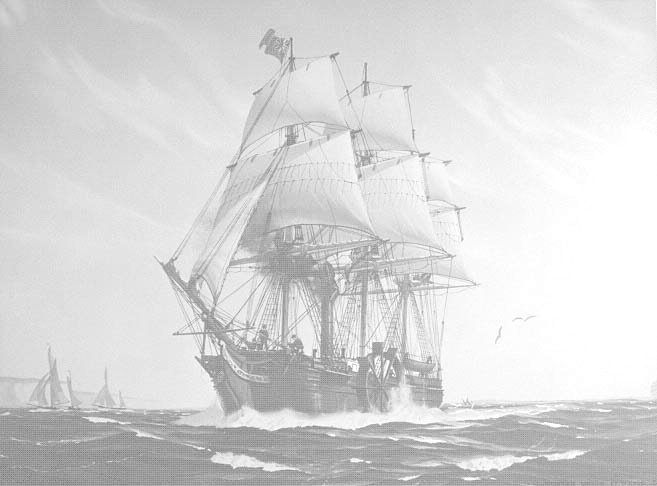
\includegraphics[width=0.7\textwidth]{images/ss_savannah.jpg}
		\end{center}
		\supercaption{\textit{SS Savannah}, première traversée atlantique à vapeur en 1819, terminée à la voile.}{Image \pd \wcfile{SS-Savannah.jpg}{par Hunter Wood, 1819}}
	\end{figure}

	Pour augmenter le rendement d’un moteur de capacité donnée, on cherche à augmenter la quantité de travail générée par chaque kilo de vapeur, qui peut être approximée par la relation~\ref{eq_travail_pdv} :

	\begin{equation*}
	w_\fromatob = - \int _{\A}^\B {p \diff v}
	\end{equation*}

	La première chose à faire est d’augmenter la pression $p_A$ de la vapeur, c’est à dire sa pression avant qu’elle ne débute sa détente dans les cylindres. Ce n’est pas chose facile : augmenter la pression de la chaudière augmente les contraintes structurelles qu’elle subit, donc son coût, et réduit son efficacité car les parois doivent être épaissies.

	On peut ensuite tenter d’augmenter le terme  $\Delta v $, c’est-à-dire la variation totale de volume lors du mouvement du piston. Autrement dit, il faut augmenter le volume balayé par les cylindres. Là encore, ce n’est pas chose facile. 
	
	D’une part, lorsque l’on augmente le diamètre des cylindres --\ ce qui augmente l’aire~$S$\ -- on soumet les pistons à une plus grande force $F_A$, pour une pression $p_A$ donnée (\ref{def_pression}) :
	\begin{equation*}
	p \equiv \frac{F}{S}
	\end{equation*}
	En augmentant la force transmise, on atteint rapidement les limites structurelles de la mécanique motrice.

	D’autre part, lorsque l’on augmente la longueur des cylindres, on rallonge également le moteur et on alourdit considérablement le mécanisme de bielle/ et vile\-brequin. D’autant que la pression et le volume de la vapeur sont liés l’un à l’autre : ils suivent approximativement une relation de type $p v^{x} = k$ pendant la détente. Autrement dit, plus le volume augmente, et plus la pression diminue : au fur et à mesure que l’on rallonge le cylindre, les gains en travail sont de plus en plus faibles.

	Le moteur \vocab{compound} répond à ce problème en utilisant plusieurs cylindres \textit{en série} (\cref{fig_cylindres_compound}). La vapeur à haute pression déplace d’abord un piston de petit diamètre (limitant ainsi la force exercée sur le mécanisme). Ensuite, elle est transférée dans un autre cylindre, de plus grand diamètre. Celui-ci permet d’obtenir une force identique avec une pression plus basse ; il balaie un plus grand volume.

	\begin{figure}
		\begin{center}
			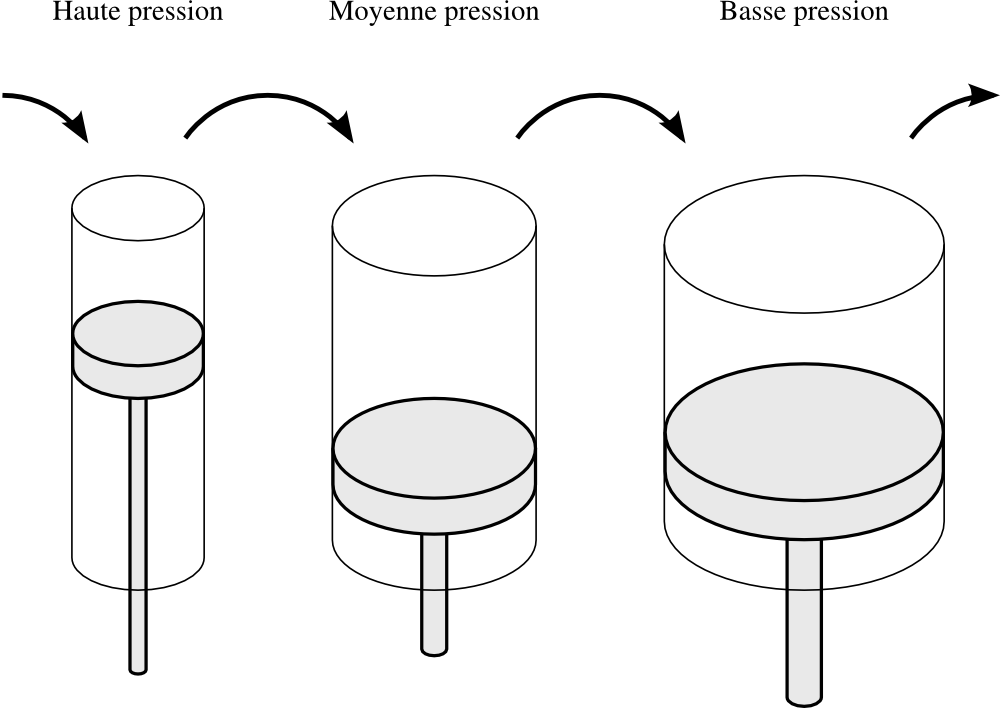
\includegraphics[width=0.8\textwidth]{images/cylindres_compound.png}
			\vspace{-1cm}
		\end{center}
		\caption{Cylindres en série, dits \textit{compound}.}
		\label{fig_cylindres_compound}
			\vspace{-0.5cm}
	\end{figure}

	Ainsi, en augmentant le volume total balayé par la vapeur en expansion, on peut extraire plus de travail de la vapeur compressée, sans surdimensionner le vilebrequin ni surcharger les pistons.

	Avec un tel moteur, la marine marchande est capable d’abandonner le cabotage : elle s’empare de la technologie qui connaît un succès immédiat. De deux cylindres en série (\vocab{double compound}) on passe à trois, et même parfois quatre (\vocab{quadruple compound}!), pour extraire à chaque fois plus d’énergie, sous forme de travail, de la vapeur.

	\begin{figure}
		\begin{center}
			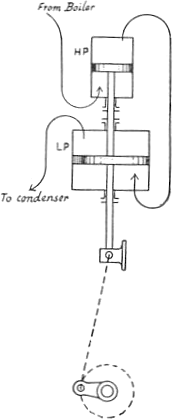
\includegraphics[height=11cm, max height=0.55\textheight]{images/ripper_compound_1.png}
			%\vspace{0.5cm}
			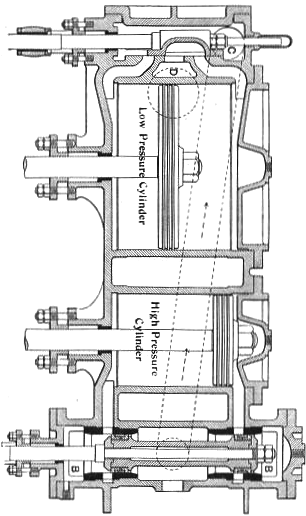
\includegraphics[height=10cm, max height=0.55\textheight]{images/ripper_compound_2.png}
		\end{center}
		\supercaption{Différents systèmes compound à vapeur.}{Images \pd \wcfile{Compound engine with both piston and slide valves (Heat Engines, 1913).png}{Prof. William Ripper, 1889}}
	\end{figure}

	L’enthousiasme gagne les armateurs, qui se targuent désormais ne plus devoir brûler qu’une feuille de papier pour déplacer une tonne de cargaison sur un mile. Même s’il s’entend que les tonnes sont unités impériales, et le papier, fort épais, l’avancée est faite. Voilà le thé des Indes bientôt dans les tasses londoniennes --\ l’empire britannique dispose des machines dont avait besoin son formidable réseau économique.
\atendofhistorysection


\renewcommand{\subtitletextcodeone}{\begin{large}} % code temporaire un peu pourri en attendant de trouver un sous-titre
\renewcommand{\nomducours}{\nomcourstrois}
\renewcommand{\sousnomducours}{\sousnomcourstrois}
\renewcommand{\chapterlabel}{chap_trois}

\olivierschapterpage{\nomducours}{\sousnomducours}

\olivierscontentpage{\contentsummarycourstrois}

\section*{Introduction}
Dans le précédent chapitre, nous avons quantifié les échanges d’énergie au sein des systèmes fermés. Ce \courstrois a pour but de répondre à une question similaire : comment quantifier les transferts d’énergie au sein d’un système lorsqu’il est traversé par un flux de masse ?
\dontbreakpage \vspace{2em}
\section{Pourquoi utiliser un système ouvert ?}
\index{système!fermé vs. ouvert}

	Dans de nombreuses machines, le fluide utilisé pour transférer de la chaleur et du travail circule de façon continue. Il peut alors être difficile d’identifier une quantité de masse fixe pour en faire un système fermé et y quantifier les transferts d’énergie. Par exemple, dans une tuyère de turboréacteur, l’air se détend et accélère continûment : à un instant donné il n’y a pas de volume identifiable qui aurait \emph{une} vitesse ou \emph{une} pression particulière.
	
	L’emploi d’un système ouvert nous est très utile pour comptabiliser l’énergie dans les flux. Plutôt que de séparer les étapes dans le temps (par exemple avant et après une compression) nous allons quantifier les transferts de travail et de chaleur en séparant les étapes dans l’espace (par exemple en amont et en aval du compresseur).

\section{Conventions de comptabilité}
\label{ch_conventions_compta_so}

	\subsection{Le système ouvert}

		\thermoquotebegin{O}
			Les difficultés de construction qui doivent être surmontées dans un moteur à gaz puissant, à cause des pressions énormes sur les pistons et de la dilatation des culasses (gare aux fissures !) sont bien connues. Une turbine à gaz sûre serait, de ce point de vue, une amélioration.
		\thermoquoteend{Aurel Stodola, 1904}{\textit{Die Dampfturbinen}~\cite{stodola1904, stodola1905}\vspace{3em}} %handmade vspace
		Nous appelons \vocab[système!ouvert, définition]{système ouvert} un sujet d’étude arbitraire dont les frontières sont perméables à la masse (\cref{fig_systeme_ouvert}). Son volume peut changer, et il peut posséder plusieurs entrées et sorties, chacune avec un débit et une pression différents.

		\onlyframabook{\begin{figure}}
		\onlyamphibook{\begin{figure}[htc]}%handmade pour poser la figure
			\begin{center}
				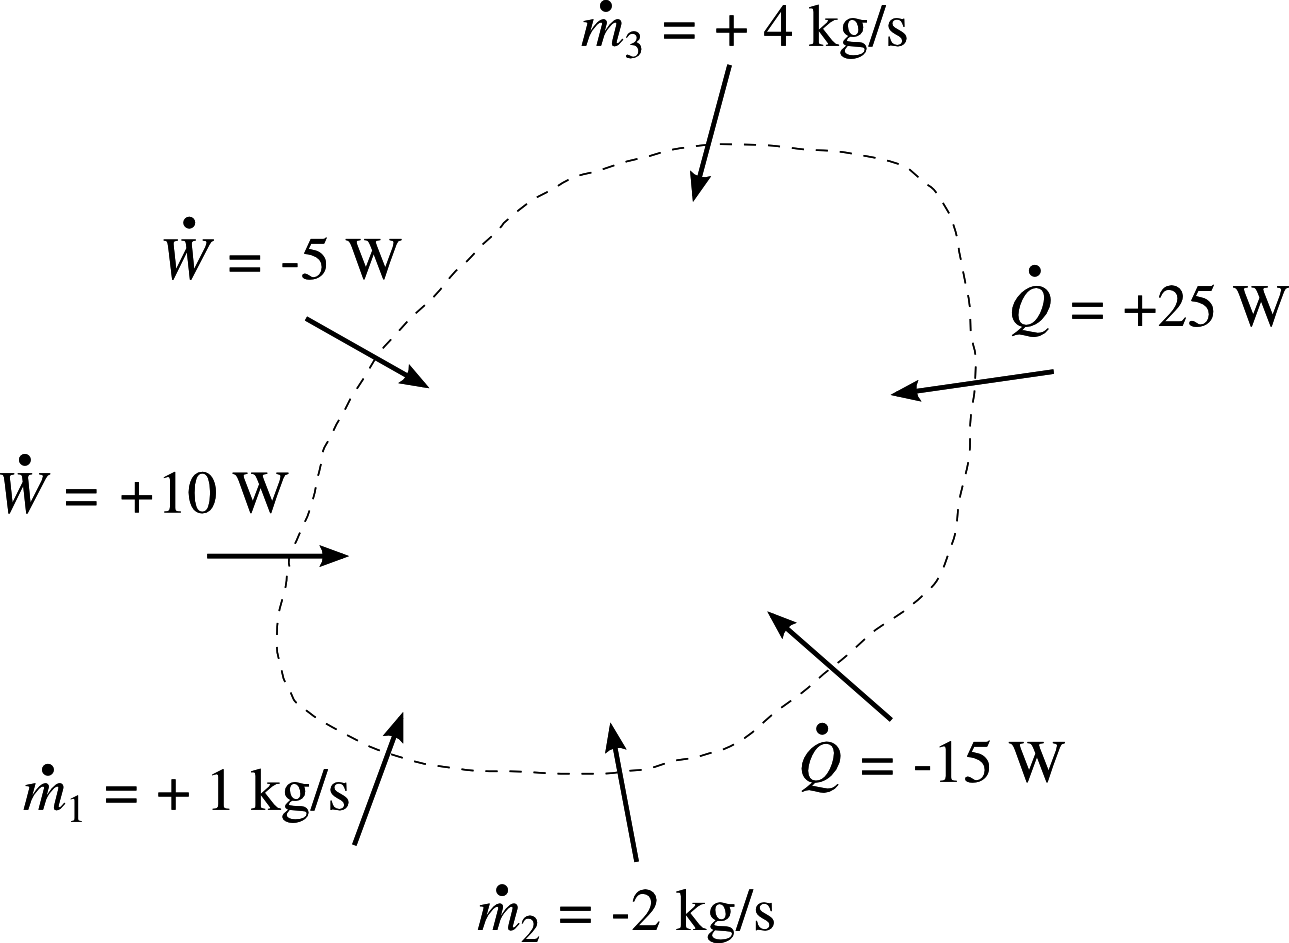
\includegraphics[width=8cm]{images/convention_systeme_ouvert.png}
			\end{center}
			\supercaption{Conventions de signe pour un système ouvert. Les flux entrants sont positifs, les flux sortants sont négatifs ; ils sont tous représentés avec des flèches rentrantes.}{schéma \cczero \oc}
			\label{fig_systeme_ouvert}
		\end{figure}

		Dans notre étude de la thermodynamique, nous n’allons utiliser que des systèmes ouverts :
		\begin{itemize}
			\item de volume fixe ;
			\item ne possédant qu’une seule entrée et qu’une seule sortie ;
			\item traversés par un débit de masse $\dot m$ constant (positif par convention).
		\end{itemize}
		Ces systèmes sont dits en \vocab{régime continu}\footnote{On dit aussi parfois \vocab[régime!permanent]{régime permanent} ou \vocab[régime!stationnaire]{stationnaire}.}.\index{continu, régime}\index{permanent, régime}\index{stationnaire, régime}

	\dontbreakpage %handmade, pour éviter un drôle de saut de page
	\subsection{Conventions de signe}

		Tout comme pour les systèmes ouverts, nous allons nous placer du point de vue du système pour quantifier les transferts :
			\begin{itemize}
				\item La réception de travail, de chaleur ou de masse se traduit par un transfert \emph{positif} ;
				\item La perte de travail, de chaleur ou de masse se traduit par un transfert \emph{négatif}.
			\end{itemize}
		
		Nous additionnons donc tous les transferts comme sur un relevé de compte en banque.


\section{Le premier principe dans un système ouvert}

	Nous avons vu que dans un système fermé le principe de conservation de l’énergie se traduisait par l’expression $q + w = \Delta u$ (\ref{eq_premier_principe_sf_maj}). Dans un système ouvert, la situation est un peu différente et nous devons tenir compte d’autres formes d’énergie.

	\subsection{Entrer et sortir du système : le travail d’écoulement}

		Imaginons un système ouvert en régime continu contenant une petite pompe à eau. Pour insérer l’eau dans la pompe à une pression donnée, il faut fournir de l’énergie au système. Au contraire, pour repousser l’eau à l’extérieur (à une pression plus haute), le système doit fournir de l’énergie. Comment quantifier cette énergie ?

		Considérons le cas d’un \vocab{élément de fluide}\index{fluide, élement de} (c’est-à-dire une petite quantité de fluide en transit, de volume $V_\text{élément}$) et qui pénètre à l’intérieur de notre système à la pression $p_1$ (\cref{fig_travail_ecoulement}).

		\begin{figure}
			\begin{center}
				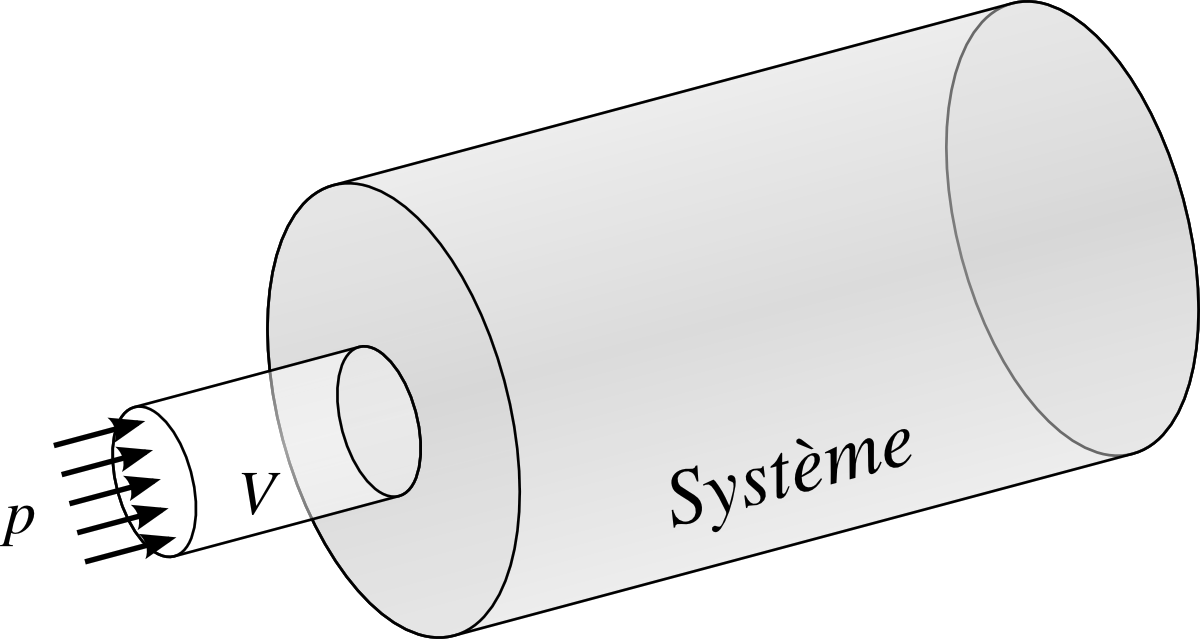
\includegraphics[width=8cm]{images/travail_insertion.png}
			\end{center}
			\supercaption{Un élément de fluide de volume $V_\text{élément}$ pénétrant à la pression~$p$ dans le système ouvert.}{schéma \cczero \oc}
			\label{fig_travail_ecoulement}
		\end{figure}

		Le travail $W_\text{insertion}$ reçu par le système lorsque l’élément est poussé à travers l’insertion est :
		\begin{IEEEeqnarray}{rCl}
			W_\text{insertion} 	& = & p_1 \ V_\text{élément}
		\end{IEEEeqnarray}
		\begin{equationterms}
			\item où \tab $W_\text{insertion}$ 	\tab est le travail d’insertion (\si{\joule}),
			\item et \tab $V_\text{élément}$ 	\tab\tab est le volume de l’élément de fluide (\si{\metre\cubed}).
		\end{equationterms}

		Si un tel volume de fluide pénètre chaque seconde dans le système, alors ce dernier reçoit une puissance sous forme de travail, que nous nommons \vocab[puissance!d’insertion]{puissance d’insertion}, $\dot{W}_\text{insertion}$. Nous l’exprimons parfois sous forme spécifique~(\S\ref{ch_valeurs_spécifiques}) :
		\begin{IEEEeqnarray}{rCl}
			\dot{W}_\text{insertion} 	& = & p_1 \ \dot{V}_1 = \dot m_1 \ p_1 \ v_1 = \dot m \ p_1 \ v_1\\
			w_\text{insertion} 			& = & p_1 \ v_1
			\label{eq_puissance_spé_insertion}	
		\end{IEEEeqnarray}
		\begin{equationterms}
			\item où \tab $\dot{W}_\text{insertion}$ 	\tab est la puissance d’insertion (\si{\watt}),
			\item 	\tab $w_\text{insertion}$ 			\tab\tab est la puissance spécifique d’insertion (\si{\joule\per\kilogram}),
			\item		\tab $\dot m_1$ 	est le débit net de masse en 1 (\si{\kilogram\per\second}),
			\item		\tab $\dot m$ 		\tab est le débit de masse traversant le système (toujours positif, \si{\kilogram\per\second}),
			\item 	\tab $\dot{V}_1$ 	\tab est le débit volumique de fluide (\si{\metre\cubed\per\second})
			\item et \tab $v_1$ 			\tab est le volume spécifique du fluide à l’entrée (\si{\metre\cubed\per\kilogram}).
		\end{equationterms}

		De la même façon, pour que le fluide sorte du système à son autre extrémité, il faut que le système fournisse continûment une puissance nommée \vocab[puissance!d’extraction]{puissance d’extraction} :
		\begin{IEEEeqnarray}{rCl}
			\dot{W}_\text{extraction} 	& = & - p_2 \ \dot{V_2} = \dot{m}_2 \ p_2 \ v_2 = - \dot{m} \ p_2 \ v_2 \\
			w_\text{extraction} 			& = & - p_2 \ v_2
		\end{IEEEeqnarray}
		\begin{equationterms}
			\item où le débit sortant $\dot m_2$ (négatif) est exprimé en fonction du débit $\dot m$ traversant le système (toujours positif, \si{\kilogram\per\second}).
		\end{equationterms}

		La somme nette de ces deux puissances aux frontières est nommée \vocab[puissance!d’écoulement]{puissance d’écoulement}, $\dot{W}_\text{écoulement} \equiv \dot{W}_\text{insertion} + \dot{W}_\text{extraction}$ . Son signe dépend des conditions d’opération -- l’étudiant/e est encouragé/e à se représenter et à formuler les conditions dans lesquelles la puissance d’écoulement peut être négative, nulle, ou positive.


	\subsection{Bilan énergétique}

		Essayons de concevoir un système ouvert en régime continu de la façon la plus générale possible, comme représenté en \cref{fig_système_ouvert}. Nous allons maintenant y comptabiliser tous les transferts d’énergie.

		\begin{figure}
			\begin{center}
				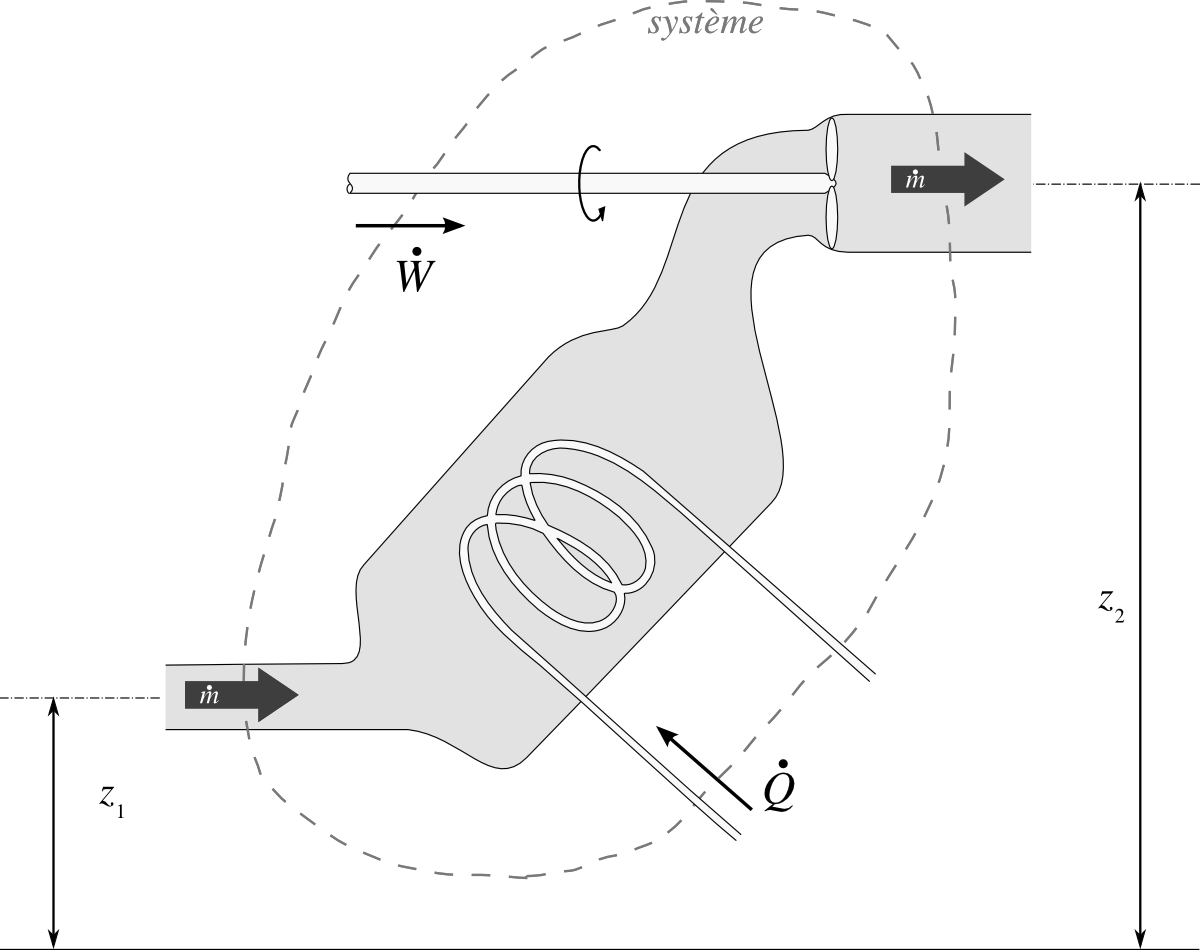
\includegraphics[width=\textwidth]{images/sfee.png}
			\end{center}
			\supercaption{Système ouvert arbitraire. Le système (dont les frontières sont en pointillés, en rouge) est traversé de gauche à droite par le fluide qui circule avec un débit de masse $\dot{m}$ constant. Il reçoit une puissance $\dot{W}_{1 \to 2}$ sous forme de travail et une puissance $\dot{Q}_{1 \to 2}$ sous forme de chaleur.}{schéma \cczero \oc}
			\label{fig_système_ouvert}
		\end{figure}

		Lorsqu’il pénètre dans le système, le fluide possède déjà une énergie interne~$u_1$ ; le système voit donc son énergie interne augmenter avec la puissance $\dot{U}_{1}$ :
		\begin{equation}
			\dot{U}_{1} = \dot{m} \ u_1
			\label{eq_w_int1}
		\end{equation}

		De même, le fluide possède une quantité d’énergie mécanique spécifique $e_\text{méca1}$ (\ref{def_énergie_mécanique_spécifique}) et le système reçoit donc également une puissance $\dot{E}_\text{méca1}$ :
		\begin{equation}
			\dot{E}_\text{méca1} = \dot m \ e_\text{méca1} = \dot{m} \ \left(\frac{1}{2} \ C_1^2 + g \ z_1\right)
			\label{eq_w_méc1}
		\end{equation}

		Ces expressions~\ref{eq_w_int1} et~\ref{eq_w_méc1} sont de signe opposé à la sortie du système, où nous leur attribuons l’indice~2.
		
		Nous avons donc fait le tour des formes d’énergie que l’on peut observer dans un système ouvert : travail d’écoulement, énergie interne, et énergie mécanique. Puisque le premier principe stipule que l’énergie est indestructible (\S\ref{ch_premier_principe}), l’ajout d’une puissance $\dot Q$ sous forme de chaleur ou $\dot W$ sous forme de travail ne peut faire varier que ces trois formes-là. Cela se traduit par l’équation :
		\begin{IEEEeqnarray}{rCl}
			\dot{Q}_{1 \to 2} + \dot{W}_{1 \to 2} + \left(\dot{W}_\text{insertion} + \dot{U}_{1} + \dot{E}_\text{méca1}\right) + \left(\dot{W}_\text{extraction} + \dot{U}_{2} + \dot{E}_\text{méca2}\right) = 0	\nonumber\\
			\label{eq_somme_puissances}
		\end{IEEEeqnarray}
		\begin{equationterms}
			\item où tous les termes sont exprimés en \si{watts}.
		\end{equationterms}

		Nous pouvons ré-exprimer l’\cref{eq_somme_puissances} en fonction de grandeurs directement mesurables :
		\begin{IEEEeqnarray}{rCl}
			\dot{Q}_{1 \to 2} + \dot{W}_{1 \to 2}  + \dot{m} \ \left(p_1 \ v_1 + u_1 + \frac{1}{2} C_1^2 + g \ z_1\right) &=& \dot{m} \ \left(p_2 \ v_2 + u_2 + \frac{1}{2} C_2^2 + g \ z_2\right)\nonumber\\
			\label{eq_grande_sfee}
		\end{IEEEeqnarray}
		ou encore :
		\begin{IEEEeqnarray}{rCl}
			\dot{Q}_{1 \to 2} + \dot{W}_{1 \to 2} 	& = & \dot{m} \left[ \Delta u + \Delta (p v) + \frac{1}{2} \Delta \left(C^2\right) + g \ \Delta z \right] 	\label{eq_grande_sfee_deltas} \\
			q_{1 \to 2} + w_{1 \to 2} 		& = & \Delta u + \Delta (p v) + \Delta e_\text{méca.}  \label{eq_petite_sfee_deltas}
		\end{IEEEeqnarray}
		\begin{equationterms}
			\item où les symboles $\Delta$ indiquent la variation des propriétés entre les points~1 et~2 du système.
		\end{equationterms}
		
		Les équations~\ref{eq_grande_sfee} et~\ref{eq_petite_sfee_deltas} sont extrêmement utiles en thermodynamique, puisqu’elles permettent de quantifier par déduction les puissances en jeu dans les écoulements. Elles nous permettent notamment de prédire les propriétés du fluide à la sortie d’un dispositif dont on connaît la puissance mécanique et les émissions de chaleur. Par exemple, on peut connaître l’énergie restante dans l’air à la sortie d’une turbine dont on connaît la puissance.
		
		\begin{anexample}
			Un compresseur de turboréacteur admet \SI{1,5}{\kilogram\per\second} d’air à une pression de~\SI{0,8}{\bar}, énergie interne de~\SI{192,5}{\kilo\joule\per\kilogram} et volume spécifique de~\SI{0,96}{\metre\cubed\per\kilogram}. Il compresse l’air jusqu’à \SI{30}{\bar}, le restituant avec une énergie interne de~\SI{542,3}{\kilo\joule\per\kilogram} et un volume spécifique de~\SI{6,19e-2}{\metre\cubed\per\kilogram}. La vitesse et l’altitude de l’air sont inchangés.
			
			Quelle est la puissance du compresseur, si ses transferts de chaleur sont négligeables ?
				\begin{answer}
					Nous appliquons l’\cref{eq_grande_sfee_deltas} pour obtenir :  $\dot{W}_{1 \to 2}
					= -\dot{Q}_{1 \to 2} + \dot{m} \left[ \Delta u + \Delta (p v) + \frac{1}{2} \Delta \left(C^2\right) + g \ \Delta z \right]
					= 0 + \dot{m} \left[ \Delta u + \Delta (p v) + 0 + 0 \right]
					= \num{1,5} \left[ (\num{542,3e3} - \num{192,5e3}) + (\num{30e5}\times\num{6,19e-2} - \num{0,8e5}\times\num{0,96})\right]
					= \SI{+6,881e5}{\watt} = \SI{+688,1}{\kilo\watt}$.
					\begin{remark}La seule difficulté dans l’application de cette équation concerne la bonne conversion des unités. Il faut toujours convertir les pressions et énergies depuis leurs unités usuelles vers des unités \textsc{si}.\end{remark}
					\begin{remark}La puissance est positive, ce qui ne nous surprend pas puisque l’air \emph{reçoit} le travail. Dans une turbine, le travail serait négatif.\end{remark}
				\end{answer}
		\end{anexample}

	\subsection{L’enthalpie}

		Dans de très nombreux cas, les termes $u$ et $p v$ varient de la même façon avec l’état du fluide%
			\footnote{Nous verrons dans le prochain chapitre que dans le cas d’un gaz parfait, ils sont tous deux proportionnels à la température.}%
		. Pour simplifier leur utilisation dans les calculs, ils sont souvent regroupés en un seul terme.

		Nous nommons la somme des termes $u$ et $p v$ l’\vocab[enthalpie!spécifique]]{enthalpie spécifique}\index{spécifique!enthalpie}, et lui attribuons le symbole~$h$ :
		\begin{equation}
			h \equiv u + p \ v
			\label{def_enthalpie}
		\end{equation}
		\begin{equationterms}
			\item où les termes sont exprimés en \si{\joule\per\kilogram}.
		\end{equationterms}

		Bien sûr, l’\vocab{enthalpie} $H$ se définit simplement comme :
		\begin{equation}
			H \equiv m \ h
		\end{equation}
		\begin{equationterms}
		      \item où \tab $H$ \tab est mesuré en \si{joules} (\si{\joule}).
		\end{equationterms}

		\thermoquotebegin{O}
			La diminution de la teneur en chaleur est égale à la valeur équivalente en chaleur du “travail utile” reçu, plus la chaleur transmise à l’extérieur plus l’augmentation en énergie cinétique par kilogramme de vapeur.
		\thermoquoteend{Aurel Stodola, 1904\\{\tiny(où la «~teneur en chaleur~» $\lambda$ n’est pas encore nommée \textit{enthalpie})}}{\textit{Die Dampfturbinen}~\cite{stodola1904, stodola1905}\vspace{1em}} %handmade vspace
		En pratique, le terme \textit{enthalpie} est souvent utilisé même s’il s’agit d’enthalpie massique ; le symbole et le contexte permettent de préciser de quelle variable il s’agit.

		En faisant usage du concept d’enthalpie, les équations~\ref{eq_grande_sfee} et~\ref{eq_petite_sfee_deltas} s’allègent pour devenir :
		\begin{IEEEeqnarray}{rCl}
			\dot{Q}_{1 \to 2} + \dot{W}_{1 \to 2} 	& = & \dot{m} \left( \Delta h + \Delta e_\text{méca.} \right) \label{eq_grande_sfee_deltas_h} \\
			q_{1 \to 2} + w_{1 \to 2} 		& = & \Delta h + \Delta e_\text{méca.}	\label{eq_petite_sfee_deltas_h}
		\end{IEEEeqnarray}

		Nous voyons ainsi que dans un système ouvert, les transferts de chaleur et de travail font varier \emph{l’enthalpie} du fluide, et non seulement son énergie interne comme dans un système fermé.

		\begin{anexample}	
			Dans une tuyère, l’air est détendu sans transfert de travail ni de chaleur. Il entre avec une enthalpie spécifique de~\SI{776}{\kilo\joule\per\kilogram} et une vitesse de~\SI[per-mode = symbol]{30}{\kilo\metre\per\hour} et ressort à même altitude, avec une enthalpie de~\SI{636}{\kilo\joule\per\kilogram}.
			
			Quelle est la vitesse d’éjection de l’air ?
				\begin{answer}
					Nous partons de l’\cref{eq_petite_sfee_deltas_h} :
						\begin{IEEEeqnarray*}{rCl}
							q_{1 \to 2} + w_{1 \to 2} 		& = & \Delta h + \Delta e_\text{méca.}\\
							\Delta e_\text{méca.} 			& = & -\Delta h + 0 + 0 \\
							\frac{1}{2}\left(C_2^2 - C_1^2\right) & = & - \Delta h\\
							C_2 &=& \left[ -2 \ \Delta h + C_1^2\right]^{\frac{1}{2}}
						\end{IEEEeqnarray*}
					Ainsi $C_2 = \left[-2\times(\num{636e3} - \num{776e3}) + \left(\frac{30}{\num{3,6}}\right)^2 \right]^{\frac{1}{2}}
						= \SI{18,7}{\metre\per\second} = \SI{67,3}{\kilo\metre\per\hour}$.
							\begin{remark}Attention aux conversions : dans les équations, les vitesses et énergies sont toujours en unités \textsc{si}.\end{remark}
							
				\end{answer}
		\end{anexample}


\section{Quantifier le travail avec un système ouvert}

	\subsection{Travail d’un fluide en évolution lente}

		Nous avons vu que lorsque le fluide évolue lentement, le travail effectué par un système fermé est quantifiable en effectuant l’intégrale $-\int p \diff v$ (\ref{eq_travail_pdv}). Avec un système ouvert, l’expression est un peu différente. Pour la développer, nous nous proposons d’étudier la compression en continu d’un fluide qui traverse un compresseur.

		Pour cela, observons tout d’abord la transformation d’une quantité de masse fixe $m_A$ circulant dans le compresseur (\cref{fig_travail_so_vu_de_sf}). En passant entre les pales en mouvement, sa pression varie de $\diff p$ et son volume de $\diff v$. Il s’agit simplement d’un système fermé qui se déplace : comme le fluide évolue très lentement (évolution réversible), le travail $\diff w_{m_\A}$ qu’elle reçoit sera :
		\begin{equation}
			\diff w_{m_\A} = -p \diff v
		\end{equation}

		\begin{figure}
			\begin{center}
				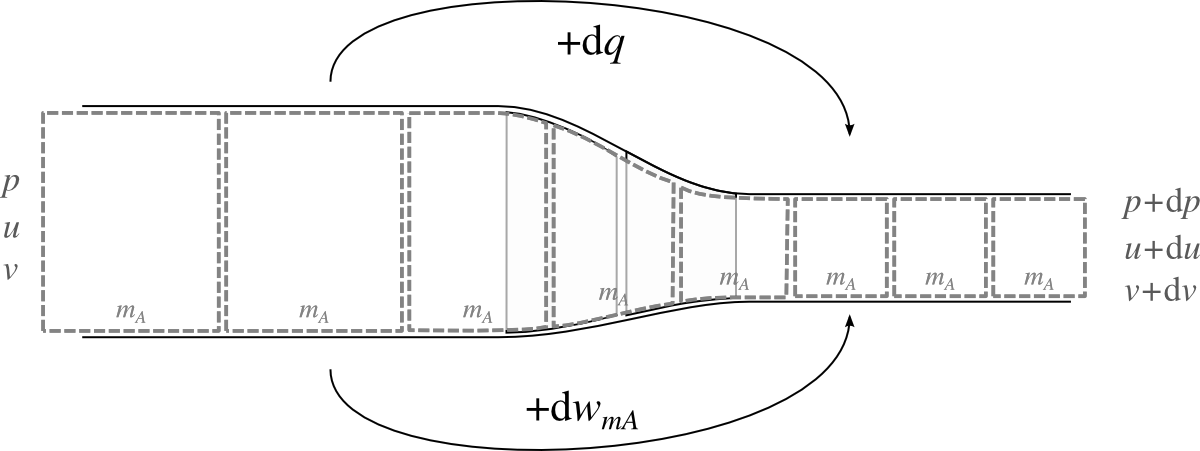
\includegraphics[width=\textwidth]{images/travail_sf_so1.png}
			\end{center}
			\supercaption{Une quantité de masse fixe $m_\A$ circule de gauche à droite à travers un compresseur. Elle est comprimée : ses propriétés passent de $p$ et $v$ à $p + \diff p$ et $v + \diff v$. Si on se place du point de vue d’un système fermé en transit, le transfert de travail est $\diff w_{m_\A} = - p \diff v$.}{schéma \cczero \oc}
			\label{fig_travail_so_vu_de_sf}
		\end{figure}

		Maintenant, observons le déroulement de ce \emph{même} phénomène du point de vue d’un système ouvert (\cref{fig_travail_so_vu_de_so}). Quelle puissance spécifique $\diff w_\text{S.0.}$ faut-il donner au compresseur pour que chaque particule de fluide reçoive un travail~$\diff w_{m_\A}$ ?

		\begin{figure}
			\begin{center}
				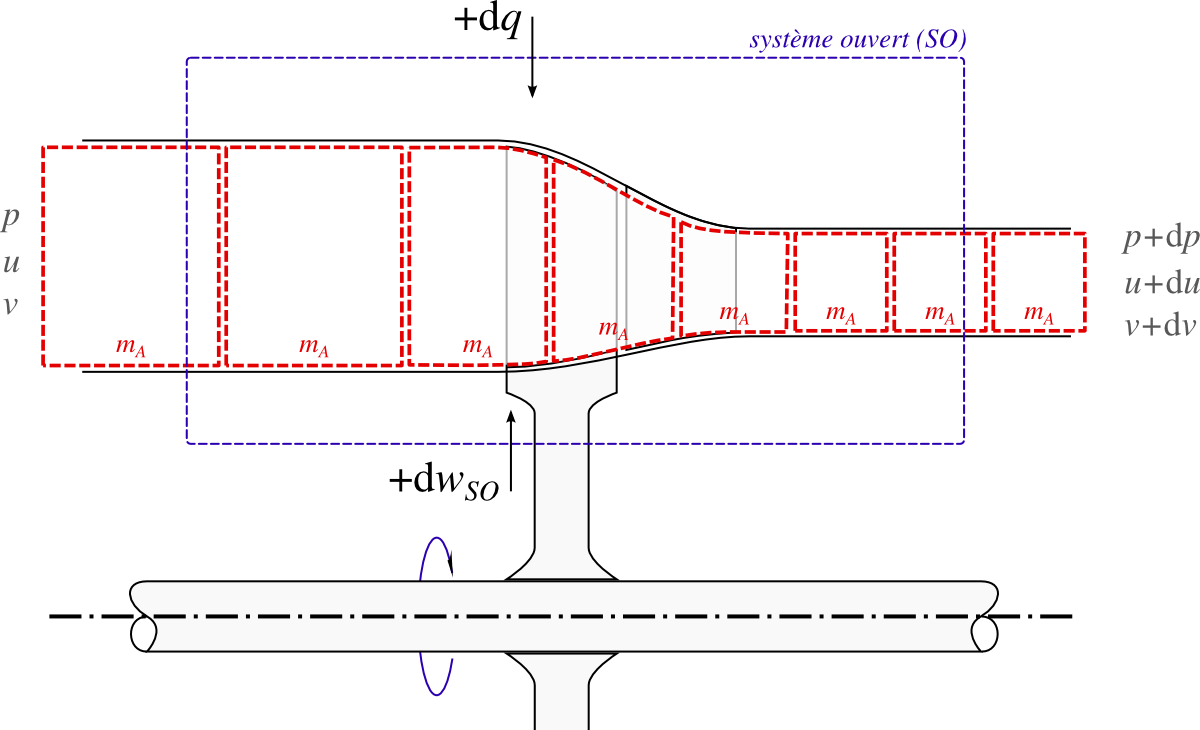
\includegraphics[width=\textwidth]{images/travail_sf_so2.png}
			\end{center}
			\supercaption{Le même écoulement qu’en \cref{fig_travail_so_vu_de_sf} observé du point de vue d’un système ouvert immobile traversé de gauche à droite par un flux continu. Nous cherchons à quantifier le travail $\diff w_\text{S.0.}$ à fournir au système pour que chaque quantité de masse $m_\A$ reçoive un travail $\diff w_{m_\A}$.}{schéma \cczero \oc}
			\label{fig_travail_so_vu_de_so}
		\end{figure}

		\clearfloats
		Le système ouvert a, lui, quatre transferts sous forme de travail :
	
		\begin{description}
			\item [La puissance spécifique d’insertion $w_\text{insertion}$] (\ref{eq_puissance_spé_insertion}) est due à l’arrivée permanente du fluide à l’entrée du système. On a, du point de vue du système ouvert :
				\begin{equation}
					w_\text{insertion} = +p \ v
				\end{equation}

			\item [La puissance spécifique de compression $-\diff w_{m_\A}$] est le travail spécifique que le système ouvert doit transférer à chaque quantité de masse $m_A$ pour qu’elle soit effectivement comprimée :
				\begin{equation}
					-\diff w_{m_\A} = -(-p \diff v)
					\label{eq_travail_so_wma}
				\end{equation}
		
			\item [La puissance spécifique d’extraction $w_\text{extraction}$] est dépensé par le système ouvert pour faire sortir continûment le fluide.
		
				À la sortie, les propriétés du fluide sont devenues $p + \diff p$ pour la pression, et $v + \diff v$ pour le volume. On a ainsi :
				\begin{equation}
					w_\text{extraction} = -(p + \diff p) (v + \diff v)
				\end{equation}
				
			\item [La puissance spécifique reçue de l’extérieur $\diff w_\text{S.O.}$] est la puissance qui alimente la compression : c’est la grandeur que nous souhaitons quantifier.

		\end{description}

		Ces quatre puissances s’annulent, car le transfert total de travail en jeu dans l’écoulement ne dépend pas du point de vue adopté :
		\begin{equation}
			\diff w_\text{S.0.} + w_\text{insertion} + \diff w_{mA} + w_\text{extraction} = 0
		\end{equation}

		On peut donc quantifier la puissance spécifique $\diff w_\text{S.0.}$ qu’il faut donner au compresseur :
		\begin{IEEEeqnarray*}{rCl}
			\diff w_\text{S.0.} 	& = & - w_\text{insertion} - \diff w_{mA} - w_\text{extraction} \\
			\diff w_\text{S.0.} 	& = & -p \ v + (-p \diff v) + (p + \diff p) (v + \diff v) \\
					& = & -p \ v - p \diff v + p \ v + p\diff v + \diff p \ v + \diff p \ \diff v \\
					& = & \diff p \ v + \diff p \ \diff v
		\end{IEEEeqnarray*}

		Et comme le multiple $\diff p \times \diff v$ tend vers zéro lorsque nous utilisons des quantités infinitésimales, nous obtenons l’expression surprenante :
		\begin{equation}
			\diff w_\text{S.0.} = v \diff p
			\label{eq_travail_vdp}
		\end{equation}

		Les termes $\diff p$ et $\diff v$ dans notre étude ne sont pas nécessairement positifs : cette expression s’applique aussi bien dans les détentes que dans les compressions, tant qu’elles sont réversibles.
	
		En intégrant cette expression \ref{eq_travail_vdp} pour l’appliquer au cas général en régime continu, nous obtenons :
		\begin{IEEEeqnarray}{rCl}
			w_\text{S.0.} 			& = & \int v \diff p 					\label{eq_travail_w_rév_so} \\
			\dot{W}_\fromatob 	& = & \dot{m} \int_\A^\B v \diff p	\label{eq_travail_W_rév_so}
		\end{IEEEeqnarray}
		\begin{equationterms}
			\item lors d’un écoulement en régime continu,
			\item lorsque l’évolution est réversible,
			\item et quel que soit l’apport de chaleur.
		\end{equationterms}

		Ainsi, lorsque nous voulons quantifier le travail dans un système ouvert, c’est l’intégrale $+\int v \diff p$, et non pas $-\int p \diff v$, qu’il nous faut calculer.
		
		Sur un diagramme pression-volume, nous pouvons visualiser ce travail en ajoutant le travail d’insertion et le travail d’extraction au travail de compression, comme montré en \cref{p-v_travail_so_construction}.

		\begin{figure}
			\begin{center}
				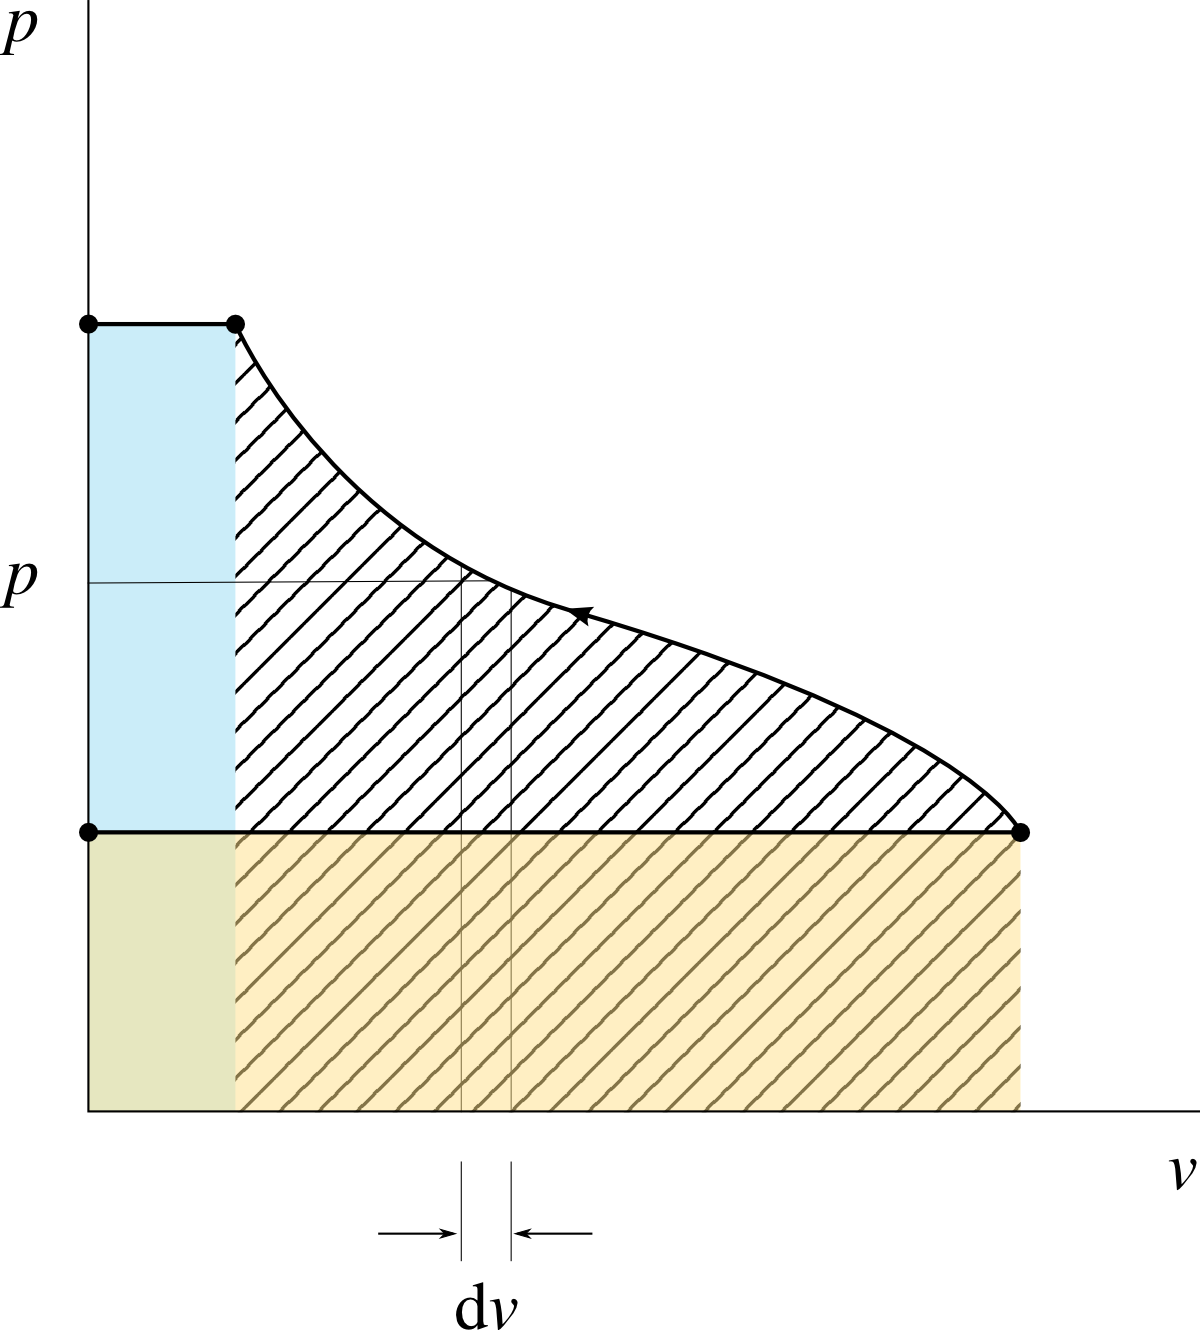
\includegraphics[width=8cm]{images/pv_systeme_ouvert_construction.png}
			\end{center}
			\supercaption{Travail reçu par un système ouvert traversé par un fluide, pendant une évolution lente.\\
			Le système reçoit d’abord le travail d’insertion ($p_\text{ini.} v_\text{ini.}$, en orange, positif) pour pénétrer dans le système,
			puis il dépense un travail de compression (aire hachurée, négative),
			et enfin il dépense le travail d’extraction ($p_\text{fin} v_\text{fin.}$, en bleu, négative).\\
			La somme nette de ces trois aires est la puissance spécifique à fournir au système ouvert.}{schéma \cczero \oc}
			\label{p-v_travail_so_construction}
		\end{figure}

		Un travail réversible effectué en régime continu se visualise donc par l’aire incluse \textit{à gauche} de la courbe, comme montré en \cref{p-v_travail_so}.

		\begin{figure}
			\begin{center}
				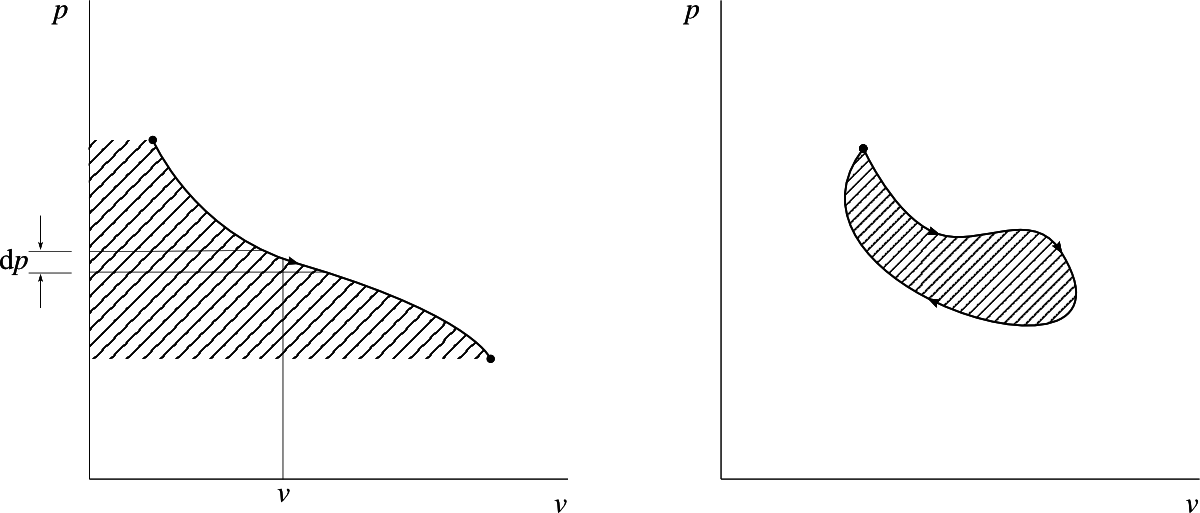
\includegraphics[width=\textwidth]{images/pv_systeme_ouvert.png}
			\end{center}
			\supercaption{Travail mesuré dans un système ouvert, pendant une évolution réversible.\\
			L’intégrale de $v \diff p$ est visualisée par l’aire à gauche de la courbe. \\
			Si le fluide revient à son état initial (ayant effectué un \vocab{cycle}), le travail développé est visualisé par l’aire incluse dans la courbe. Dans ce cas, la quantification est identique en système fermé et ouvert.}{schéma \cczero \oc}
			\label{p-v_travail_so}
		\end{figure}

		\begin{anexample}
			Une pompe à liquide compresse lentement un débit d’eau de~\SI{2}{\kilogram\per\second} depuis \SI{1}{\bar} jusqu’à \SI{20}{\bar}. Pendant la compression, le volume spécifique de l’eau reste constant à $v_L = \SI{e-3}{\metre\cubed\per\kilogram}$. Quelle est la puissance consommée sous forme de travail ?
				\begin{answer}
					Sur un diagramme pression-volume et de façon qualitative (c’est-à-dire sans représenter les valeurs numériques), l’évolution peut être représentée ainsi :
							\begin{center}
								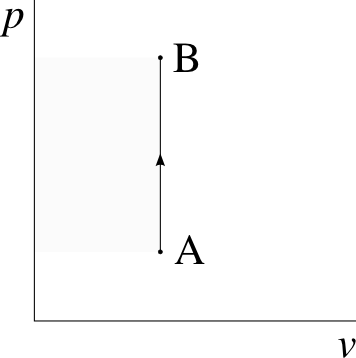
\includegraphics[width=3cm]{images/exe_pv_isochore_so.png}
							\end{center}
					Nous utilisons l’\cref{eq_travail_W_rév_so} en prenant garde aux unités. Comme $v$ est indépendant de $p$, l’intégration se fait sans peine : $\dot{W}_\fromatob 	= \dot{m} \int_\A^\B v \diff p = \dot{m} \ v_L \int_\A^\B \diff p = \dot{m} \ v_L \left[p\right]_{p_\A}^{p_\B} = 2 \times \num{e-3} \left(\num{20e5} - \num{1e5}\right) = \SI{+3,8e3}{\watt} = \SI{+3,8}{\kilo\watt}$.
				\end{answer}
					\begin{remark}Cette puissance est bien positive : c’est le fluide dans le système qui reçoit du travail.\end{remark}
					\begin{remark}Ici le volume spécifique $v_L$ est constant (comme toujours avec l’eau liquide). Si c’était la pression qui était constante, alors le travail serait nul même si $v$ était amené à varier.\end{remark}
		\end{anexample}
		
		\begin{anexample}
			Un compresseur compresse lentement un débit d’air de~\SI{2}{\kilogram\per\second} depuis \SI{1}{\bar} jusqu’à \SI{20}{\bar}. Pendant la compression, le volume spécifique et la pression de l’air sont liés par la relation $p \ v^{\num{1,35}} = k$. À l’entrée, le volume spécifique de l’air est de $v_\A = \SI{0,8}{\metre\cubed\per\kilogram}$.\\
			Quelle est la puissance consommée sous forme de travail ?
				\begin{answer}
				Sur un diagramme pression-volume et de façon qualitative, l’évolution peut être représentée ainsi :
							\begin{center}
								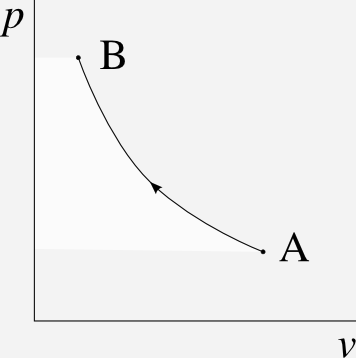
\includegraphics[width=3cm]{images/exe_pv_exp_so.png}
							\end{center}
					Ici le volume spécifique est fonction de la pression : nous avons $v = \left(\frac{k}{p}\right)^{\frac{1}{\num{1,35}}} = k^{\frac{1}{\num{1,35}}} p^{-\frac{1}{\num{1,35}}}$.\\
					Nous partons de l’\cref{eq_travail_W_rév_so} : $\dot{W}_\fromatob
					= \dot{m} \int_\A^\B v \diff p
					= \dot{m} \ k^{\frac{1}{\num{1,35}}} \int_\A^\B p^{-\frac{1}{\num{1,35}}} \diff p
					= \dot{m} \ k^{\frac{1}{\num{1,35}}} \left[\frac{1}{-\frac{1}{\num{1,35}} +1} p^{-\frac{1}{\num{1,35}} +1}\right]_{p_\A}^{p_\B}
					= \dot{m} \ \left(p_\A v_\A^{\num{1,35}}\right)^{\frac{1}{\num{1,35}}} \frac{1}{\num{0,25926}} \left[p^{\num{0,25926}}\right]_{p_\A}^{p_\B}
					= 2 \left(\num{20e5} \times \num{0,8}^{\num{1,35}}\right)^{\frac{1}{\num{1,35}}} \frac{1}{\num{0,25926}} \left[\left(\num{20e5}\right)^{\num{0,25926}} - \left(\num{1e5}\right)^{\num{0,25926}}\right]
					= \SI{+6,666e6}{\watt} = \SI{+6,666}{\mega\watt}$.
				\end{answer}
					\begin{remark}Ici la clé est de bien décrire la fonction $v_{(p)}$ avant de procéder à l’intégration.\end{remark}
					\begin{remark}La puissance du compresseur est \num{1700} fois plus grande que celle de la pompe de l’exemple précédente. De plus, le volume spécifique de l’air à l’entrée est \num{800} fois plus grand : il faudra une machine de taille beaucoup plus importante (elle doit absorber un débit volumique $\dot{V}_\A = \dot{m} \ v_\A = \SI{1,6}{\metre\cubed\per\second} = \SI{1600}{\liter\per\second}$ à l’entrée).\end{remark}
		\end{anexample}


	\subsection{Travail d’un fluide en évolution rapide}
	
		Lorsque le fluide évolue de façon rapide (ce qui est toujours le cas en pratique), nous retrouvons les phénomènes que nous avons décrits au chapitre précédent (\S\ref{ch_évolutions_irr_sf}) : la pression exercée sur les parois mobiles ne correspond plus à la pression «~moyenne~» à l’intérieur du fluide. Le travail à fournir dans les compressions est plus grand et le travail réceptionné pendant les détentes est plus faible que lors des évolutions lentes.
		
		Le fait d’utiliser un système ouvert pour comptabiliser les transferts d’énergie ne change bien sûr rien au problème. Nous n’avons pas les moyens de prédire analytiquement le travail à fournir pour une compression à une vitesse donnée. Le problème –calculer la distribution spatiale de la pression à l’intérieur du fluide en fonction du temps– relève de la mécanique des fluides, et sera quoi qu’il en soit résolu au cas-par-cas.
		
		Sur nos diagrammes pression-volume, nous représentons les évolutions irréversibles avec un trait en pointillés, pour bien les différencier des évolutions réversibles (\cref{fig_pv_evolution_irr_so}).
		
		\onlyframabook{\begin{figure}[htc]}%handmade
		\onlyamphibook{\begin{figure}}
			\begin{center}
				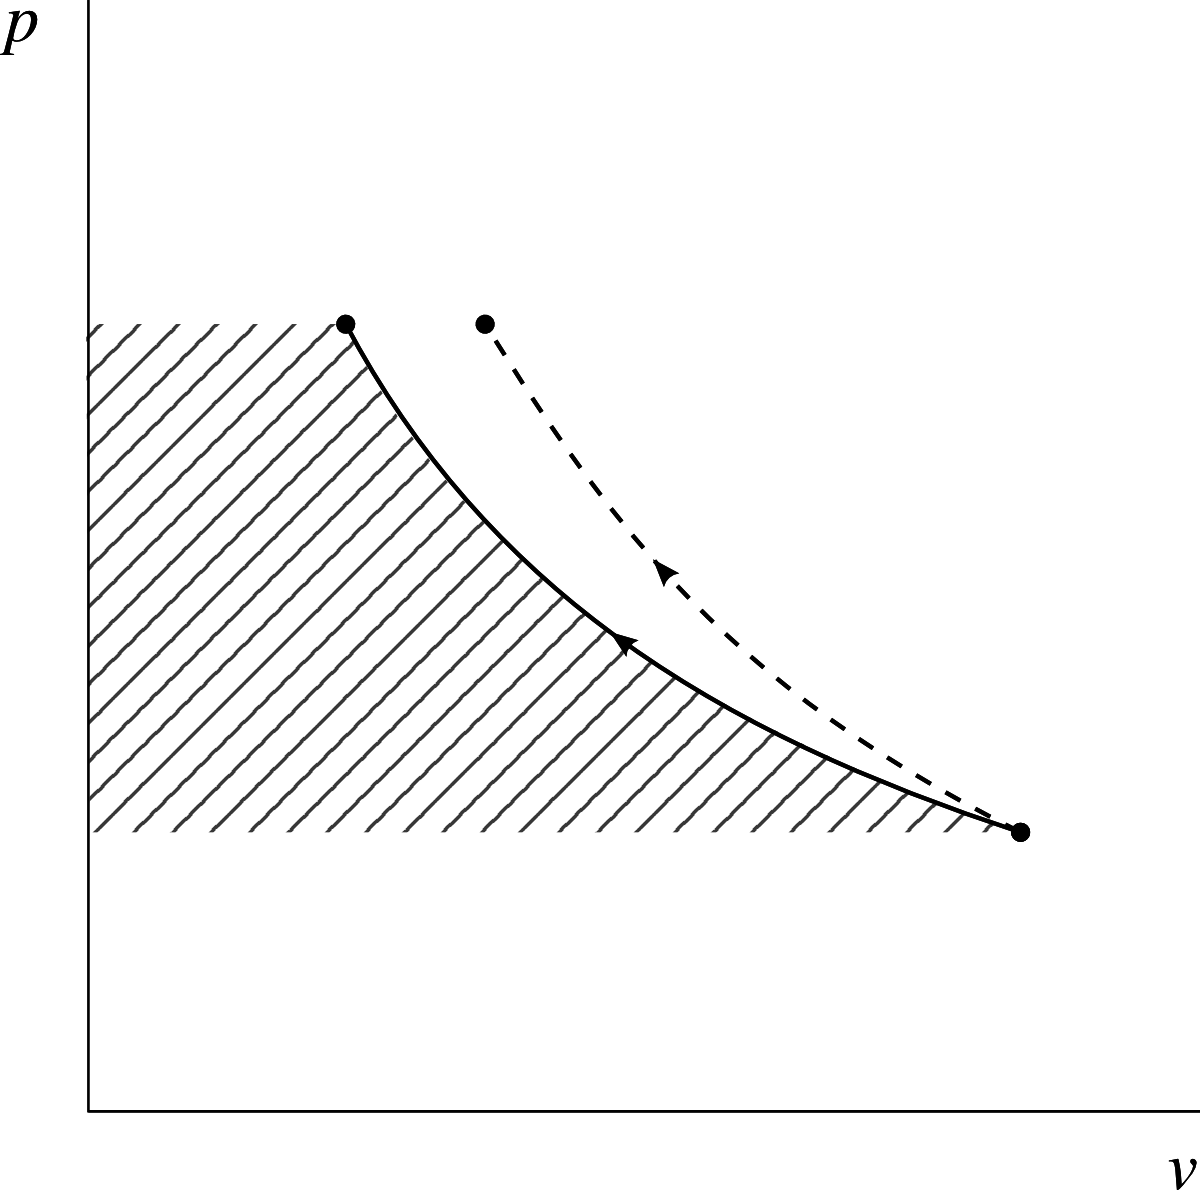
\includegraphics[width=8cm]{images/pv_compression_irreversible_so.png}
			\end{center}
			\supercaption{Compressions réversible (trait continu) et irréversible (en pointillés) représentées sur un diagramme pression-volume. Dans un système ouvert, les transferts de travail peuvent être visualisés avec l’aire à gauche de la courbe, mais uniquement lorsque les évolutions sont réversibles.}{schéma \cczero \oc}
			\label{fig_pv_evolution_irr_so}
		\end{figure}
	
		\clearfloats %handmade
		\begin{anexample}
			De l’air est compressé en continu de 1 à~\SI{20}{\bar} dans un compresseur. Dès la sortie du compresseur l’air rentre dans une turbine qui le détend de 20 à~\SI{1}{\bar}. Dès la sortie de la turbine, l’air est à nouveau inséré dans le compresseur.
			
			Quelle sera l’allure des évolutions sur un diagramme pression-volume ?
					\begin{answer}
						Si les évolutions se font lentement, la pression et le volume spécifique passent toujours par les mêmes valeurs pendant les allers-retours :
							\begin{center}
								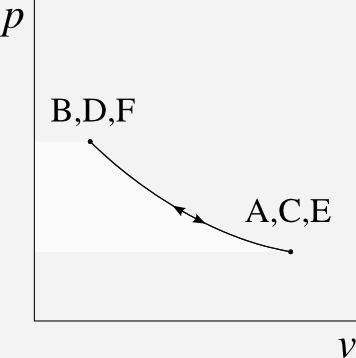
\includegraphics[height=3cm]{images/exe_pv_rev_so.png}
							\end{center}
						En revanche, si les évolutions sont rapides, à chaque trajet le volume spécifique final est plus grand que ce qu’il aurait été pendant un trajet lent :
							\begin{center}
								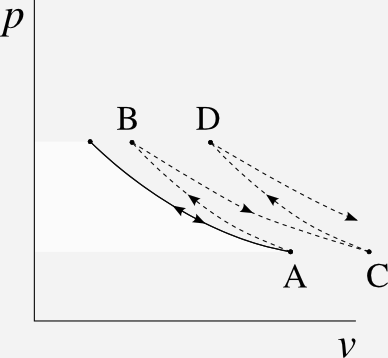
\includegraphics[height=3cm]{images/exe_pv_irr_so.png}
							\end{center}
						Ainsi, les propriétés se décalent progressivement sur le diagramme pression-volume. Si les évolutions ne se font pas lentement, le compresseur demande plus de travail que la turbine est capable de fournir au retour. Cet excédent de travail consommé par l’air augmente son énergie interne et sa température.
					\end{answer}

		\end{anexample}
	
\section{Quantifier la chaleur avec un système ouvert}

	Avec un système ouvert nous allons utiliser la même méthode qu’avec un système fermé : comme nous ne savons pas quantifier les transferts de chaleur directement, nous allons toujours procéder par déduction.
	Mathématiquement, nous ne faisons que réutiliser l’\cref{eq_grande_sfee_deltas_h} pour obtenir :
	\begin{IEEEeqnarray}{rCl}
		\dot{Q}_{1 \to 2} & = & \dot{m} \left( \Delta h + \Delta e_\text{méca.}\right) - \dot{W}_{1 \to 2} \\
			q_{1 \to 2} 	& = & \Delta h + \Delta e_\text{méca.}  - w_{1 \to 2}
	\end{IEEEeqnarray}
	\begin{equationterms}
		\item pour un système ouvert.
	\end{equationterms}
		
		Là encore, toute la difficulté pour quantifier un transfert de chaleur est de prédire et quantifier le changement de l’enthalpie, $\Delta h$. Pour les gaz, $h$ est quasiment proportionnelle à la température ; pour les liquides et vapeurs, la relation est plus complexe. Nous apprendrons à quantifier l’enthalpie dans les fluides aux \coursquatre et \courscinq.


\renewcommand{\nomducours}{\nomcoursquatre}
\renewcommand{\sousnomducours}{\sousnomcoursquatre}
\renewcommand{\chapterlabel}{chap_quatre}

\olivierschapterpage{\nomducours}{\sousnomducours}

\olivierscontentpage{\contentsummarycoursquatre}

\section*{Introduction}
Au cours des chapitres~\deux et~\trois nous avons appris à quantifier les transferts d’énergie, mais nous ne pouvons le faire que si nous connaissons les valeurs de $u$ ou de $h$, propriétés qu’il est impossible de mesurer directement en pratique.
	
Ce \coursquatre se propose de répondre à deux questions :
\begin{itemize}
	\item Comment peut-on décrire le comportement de l’air lorsqu’il est chauffé ou comprimé ?
	\item Comment peut-on prévoir les valeurs de $u$ et de $h$ lorsqu’on utilise de l’air ?
\end{itemize}
Ce chapitre est incompatible avec le \courscinq, où nous devrons oublier tout ce qui est appris ici.
\dontbreakpage \vspace{2em}
\section{Définition}

	\subsection{Le manomètre comme thermomètre}
	\label{ch_le_manomètre_comme_thermomètre}

		Commençons par le plus important :

		\begin{trucimportant}
			Le gaz parfait est un \textit{modèle mathématique},\linebreak
			permettant de prédire la température d’un gaz en fonction de sa pression.
		\end{trucimportant}

		Le modèle du gaz parfait définit de lui-même une échelle de température. On propose de mesurer très simplement la température absolue $T$ avec un manomètre, en stipulant qu’elle est directement proportionnelle à la pression $p$ et inversement proportionnelle à la masse volumique $\rho$.

		On peut ainsi dire que le gaz parfait ne décrit pas la réalité des choses, que ce n’est pas un principe physique, mais bien seulement un modèle simplifié du comportement des gaz. Sa plage de validité est limitée et floue.



		\subsection{Définition : l’équation d’état}

				\thermoquotebegin{O}
			Le changement de température occasioné dans les gaz par le changement de volume peut être regardé comme l’un des faits les plus importans de la physique, à cause des nombreuses conséquences qu’il entraîne, et en même temps comme l’un des plus difficiles à éclaircir et à mesurer par des expériences décisives. Il semble présenter dans plusieurs circonstances des anomalies singulières.\nolinebreak\makebox(18,5){\color{gray}\scalebox{2}{»}}\par\vspace{-0.3cm}\begin{flushright}Sadi Carnot, 1824~\cite{carnot1824}\end{flushright}
		\makebox(18,5){\color{gray}\scalebox{2}{«}}
		M. S. Carnot, évitant l’emploi de l’analyse mathématique, arrive par une série de raisonnemens délicats et difficiles à saisir, à des résultats qui se déduisent sans peine d’une loi plus générale, que je vais chercher à établir.
		\thermoquoteend{Émile Clapeyron, 1834~\cite{clapeyron1834}}{}
		Nous appellerons \vocab{gaz parfait} (ou \vocab{gaz idéal}) un fluide à l’état gazeux dont le multiple de la pression et du volume, $p v$, reste proportionnel à sa température. La constante de proportionnalité est nommée \vocab{constante du gaz}, et notée $R$ ; elle dépend de la nature du~gaz.
		\begin{equation}
			p v = R T
			\label{eq_pv=RT}
		\end{equation}
		\begin{equationterms}
			\item par définition pour un gaz parfait,
			\item où \tab $p$ \tab est la pression (\si{\pascal}),
			\item 	\tab $v$ \tab le volume spécifique (\si{\metre\cubed\per\kilogram}),
			\item 	\tab $T$ \tab la température (\si{\kelvin}),
			\item et \tab $R$ \tab la constante du gaz considéré (\si{\joule\per\kelvin\per\kilogram}).
		\end{equationterms}

		L’\cref{eq_pv=RT} est nommée \vocab{équation d’état des gaz parfaits}. Elle peut également être exprimée en fonction de la masse :
		\begin{equation}
			p V = m R T
			\label{eq_pV=mRT}
		\end{equation}
		\begin{equationterms}
			\item où \tab $V$ \tab est le volume (\si{\metre\cubed}),
			\item et \tab $m$ \tab la masse de gaz considérée (\si{\kilogram}).
		\end{equationterms}
		
		Il est aussi possible d’exprimer l’\cref{eq_pV=mRT} en fonction de la quantité de matière en \si{moles}.\footnote{Dans les ouvrages tels que celui d’Alexandre Watzky~\cite{watzky2007}, la constante en \si{\joule\per\kelvin\per\kilogram} est notée $r$. La grandeur notée $R = \SI{8,3143}{\joule\per\kelvin\per\mole}$ est universelle, et les gaz adoptent des valeurs de $r$ différentes en fonction de leur masse molaire $M \equiv \frac{m}{n}$. Dans le présent ouvrage, nous ne quantifions pas les quantités de matière.}
		 Parce qu’elle est indissociable du concept de température absolue, il a fallu 150 ans pour que cette équation prenne sa forme définitive : celle que lui a donnée \wf{Émile Clapeyron} en 1834~\cite{clapeyron1834}.

			\begin{anexample}
				Une masse de~\SI{2}{\kilogram} de gaz dont la constante est $R = \SI{100}{\joule\per\kelvin\per\kilogram}$ est contenue dans un réservoir de~\SI{200}{\liter} à pression de~\SI{3}{\bar}. Quelle est sa température ?
				\begin{answer}
					Nous partons de l’\cref{eq_pV=mRT} pour exprimer la température : $T = \frac{p \ V}{m \ R} = \frac{\num{3e5} \times \num{0,2}}{2 \times \num{100}} = \SI{300}{\kelvin} = \SI{26,85}{\degreeCelsius}$.
				\end{answer}
					\begin{remark}Admirable Émile ! La simplicité de ce calcul nous manquera au chapitre prochain.\end{remark}
					\begin{remark}La seule épine dans cette équation concerne les unités, qu’il faut bien convertir en \textsc{si} : $\SI{200}{\liter} = \SI{0,2}{\metre\cubed}$ et $\SI{3}{\bar} = \SI{3e5}{\pascal}$. La température est toujours en \si{kelvins}. \end{remark}
			\end{anexample}

			\begin{anexample}
				L’air atmosphérique peut être modélisé par un gaz parfait avec $R_\text{air} = \SI{287}{\joule\per\kilogram\per\kelvin}$. Aux conditions ambiantes (\SI{1}{\bar}, \SI{20}{\degreeCelsius}), quels sont le volume spécifique et la masse volumique de l’atmosphère ?
				\begin{answer}
					Nous partons de l’\cref{eq_pv=RT} pour exprimer le volume spécifique : $v = \frac{R \ T}{p} = \frac{\num{287} \times (\num{20} + \num{273,15})}{\num{1e5}} = \SI{0,841}{\metre\cubed\per\kilogram}$. La masse volumique suit simplement : $\rho = \frac{1}{v} = \SI{1,189}{\kilogram\per\metre\cubed}$.
				\end{answer}
					\begin{remark}Là encore, une erreur dans les unités de température serait fatale (on s’en convaincra en prenant $T = \SI{0}{\degreeCelsius}$).\end{remark}
					\begin{remark}Dans un mètre cube nous n’avons que \SI{1,2}{\kilogram} d’air. C’est très peu, surtout si l’on compare à l’eau liquide (\SI{1000}{\kilogram} pour le même volume). Les machines à air fonctionnent usuellement avec des débits volumiques importants.\end{remark}
			\end{anexample}


	\subsection{Que représente un gaz parfait ?}
	\label{ch_gaz_parfait_kezako}

		Le gaz parfait est le modèle le plus simple que l’on puisse imaginer pour représenter le comportement d’un gaz.
		
		Selon ce modèle, les molécules se comportent comme des sphères rebondissant les unes contre les autres (\cref{fig_gaz_boules}). On peut imaginer un grand nombre de très petites boules de billard en mouvement chaotique, qui se percutent et rebondissent les unes contre les autres sans jamais s’attirer ni dissiper leur énergie par frottement.
		
		\begin{figure}
			\begin{center}
				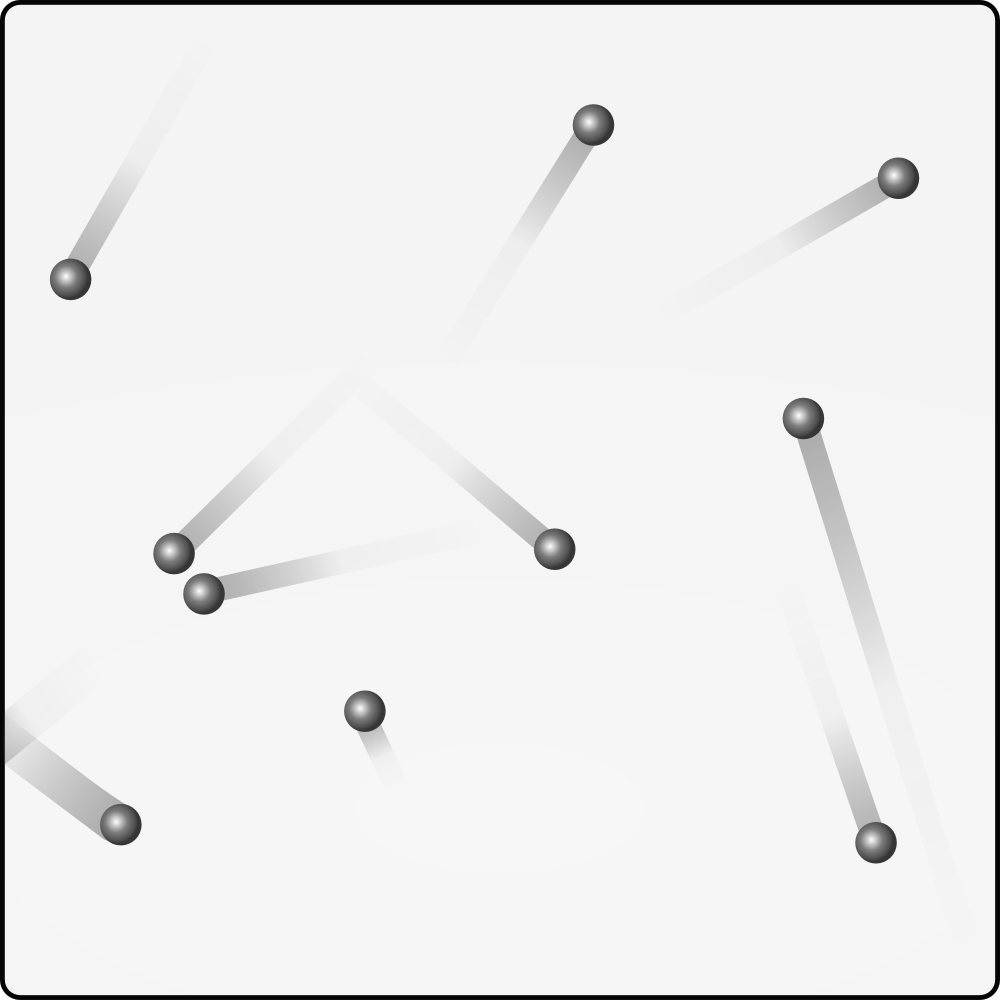
\includegraphics[width=8cm]{images/gaz_boules.png}
			\end{center}
			\supercaption{Un gaz parfait peut être visualisé comme un ensemble de boules en mouvement désordonné. Elles se percutent sans frottement et sans attraction mutuelle. La vitesse de chaque boule change à chaque heurt.}%
			{Dérivé d’\wcfile{Kinetic_theory_of_gases.svg}{un schéma} \ccbysa par \wcu{Sharayanan}}
			\label{fig_gaz_boules}
		\end{figure}
		
		Dans ce chaos, la température est une mesure de l’énergie cinétique des molécules. On la quantifie en mesurant la force résultant de l’impact des molécules sur une paroi du récipient --\ c’est-à-dire avec la pression. Avec ce modèle, nous pouvons proposer une échelle de température telle que $T \propto p$.
		
		Plus le nombre de molécules impactant la surface est faible, plus il faut qu’elles l’impactent fortement pour générer une pression donnée. Ainsi, lorsque la masse volumique $\rho$ diminue à une pression donnée, c’est que la température augmente. On peut donc également proposer $T \propto \frac{1}{\rho}$.
		
		Si ces deux propositions sont réunies en une seule équation, nous obtenons un modèle simple pour quantifier la température : $T \propto p v$.
		
		
	\subsection{Que ne représente pas un gaz parfait ?}
	\label{ch_pas_gaz_parfait}
	
		\thermoquotebegin{O}
			Quiconque veut étudier les propriétés de la matière dans un problème réel peut désirer partir en écrivant les équations fondamentales et puis essayer de les résoudre mathématiquement. Bien qu’il y ait des gens qui essayent d’emprunter une telle approche, ces personnes sont des ratés de ce domaine ; les véritables réussites sont le fait de ceux qui partent d’un point de vue \emph{physique}, de ceux qui ont une idée approximative de l’endroit où ils vont et qui commencent en faisant la bonne approximation, sachant ce qui est grand et ce qui est petit dans une situation donnée qui est compliquée.
		\thermoquoteend{Richard Feynman, 1963}{\textit{The Feynman Lectures on \mbox{Physics}} \mbox{\cite{feynman1963, feynman1963fr}}}
	
		Le comportement des molécules lorsqu’elles sont proches les unes des autres est en réalité très complexe, car les forces d’attraction y jouent un rôle déterminant. L’influence de ces forces est d’autant plus grande que les molécules sont lentes et structurellement complexes (l’interaction entre deux molécules d’hydrocarbone, par exemple, est plus difficile à modéliser que l’interaction entre deux molécules d’hélium).

		Les conséquences à l’échelle macroscopique de ces interactions, et les conditions dans lesquelles elles ne doivent plus être négligées, font l’objet du \courscinq.

		Nous retiendrons pour l’instant que le modèle du gaz parfait fonctionne mieux :

		\begin{itemize}
			\item Lorsque les molécules se percutent à grande vitesse, c’est-à-dire lorsque la température du gaz est élevée ;
			\item Lorsque l’espace moyen entre les molécules est grand, c’est-à-dire lorsque le volume spécifique du gaz est grand.
		\end{itemize}
		
		Ces conditions permettent de s’assurer que les forces d’attraction entre molécules gardent un rôle mineur dans le comportement global du gaz. Elles sont respectées pour l’air dans la grande majorité des applications en ingénierie. Nous utiliserons la valeur $R_\text{air} = \SI{287}{\joule\per\kilogram\per\kelvin}$ pour l’air pur dans nos machines.


	\subsection{Limites du modèle}

		Il ne faudra pas longtemps à l’étudiant/e pour trouver les limites de l’\cref{eq_pV=mRT}, qui indique qu’une masse non-nulle de gaz parfait occupe \textit{un volume nul} à température nulle. Strictement parlant, le gaz parfait ne peut pas exister --\ le modèle mathématique perd son sens à très basse température puisqu’il ne tient pas compte du volume des molécules elles-mêmes.

		Plusieurs autres équations d’état peuvent être utilisées pour correspondre aux gaz réels sur une plus grande plage de propriétés.

		Ainsi, l’\vocab{équation de Van der Waals}, proposée dès la fin du \textsc{xviii}\ieme siècle, propose :
		\begin{equation}
			\left(p + \frac{a}{v ^2}\right) (v - b) = R T
		\end{equation}
		\begin{equationterms}
			\item où $a$ et $b$ sont deux constantes.
		\end{equationterms}

		Cette équation a l’intérêt de tenir compte de deux facteurs ignorés dans l’équation d’état~\ref{eq_pv=RT} : la force d’attraction entre les molécules (le terme $a/v^2$, qui devient partie de l’expression de la pression) et le volume occupé par les molécules elles-mêmes (le terme $b$ qui se retranche au volume disponible).

		Malgré les difficultés inhérentes à la quantification des termes $a$ et $b$, ces modifications ont considérablement étendu la plage d’application des équations d’état. Elles ont valu à leur auteur, \wf{Johannes Diderik van der Waals}, le prix Nobel de physique en 1910.

		La recherche de modèles mathématiques pour décrire l’état des gaz réels est un thème important de recherche en mécanique des fluides. L’étudiant/e curieux/se pourra consulter les équations d’état \wed{Real_gas\#Beattie.E2.80.93Bridgman_model}{de Beattie-Bridgeman}, \wed{Benedict\%E2\%80\%93Webb\%E2\%80\%93Rubin_equation}{de Benedict-Webb-Rubin} ou encore de Strobridge pour se faire un aperçu de la complexité croissante de cette branche. Nous resterons quant à nous à l’\cref{eq_pv=RT}.



\section{Propriétés des gaz parfaits}

	\subsection{Deux capacités calorifiques importantes}

		Nous avons déjà abordé la notion de capacité calorifique (ou «~chaleur massique~»), au premier chapitre (\ref{eq_def_capacité_calorifique_massique}). Elle se définit comme la quantité de chaleur nécessaire pour augmenter d’un Kelvin\footnote{Ou d’un degré Celsius, ces différences de température étant égales.}
		la température d’un kilo du corps. On a ainsi :
		\begin{equation}
			c = \frac{\diff q}{\diff T}
		\end{equation}
		\begin{equationterms}
			\item où \tab $c$ 		\tab\tab est la capacité calorifique spécifique (\si{\joule\per\kelvin\per\kilogram}),
			\item 	\tab $\diff q$ \tab la quantité infinitésimale de chaleur spécifique fournie (\si{\joule\per\kilogram}),
			\item et \tab $\diff T$ \tab la variation infinitésimale de température provoquée (\si{\kelvin}).
		\end{equationterms}

		Comme la température d’un gaz varie aussi lorsqu’il reçoit ou fournit du travail, il existe une infinité de façons de faire varier sa température d’un degré, en combinant chaleur et travail (\cref{fig_expérience_diff_chaleurs_massiques}). Chacune nécessite une quantité de chaleur unique ; il y a donc \textit{une infinité de chaleurs massiques} correspondantes.

		\begin{figure}
			\begin{center}
				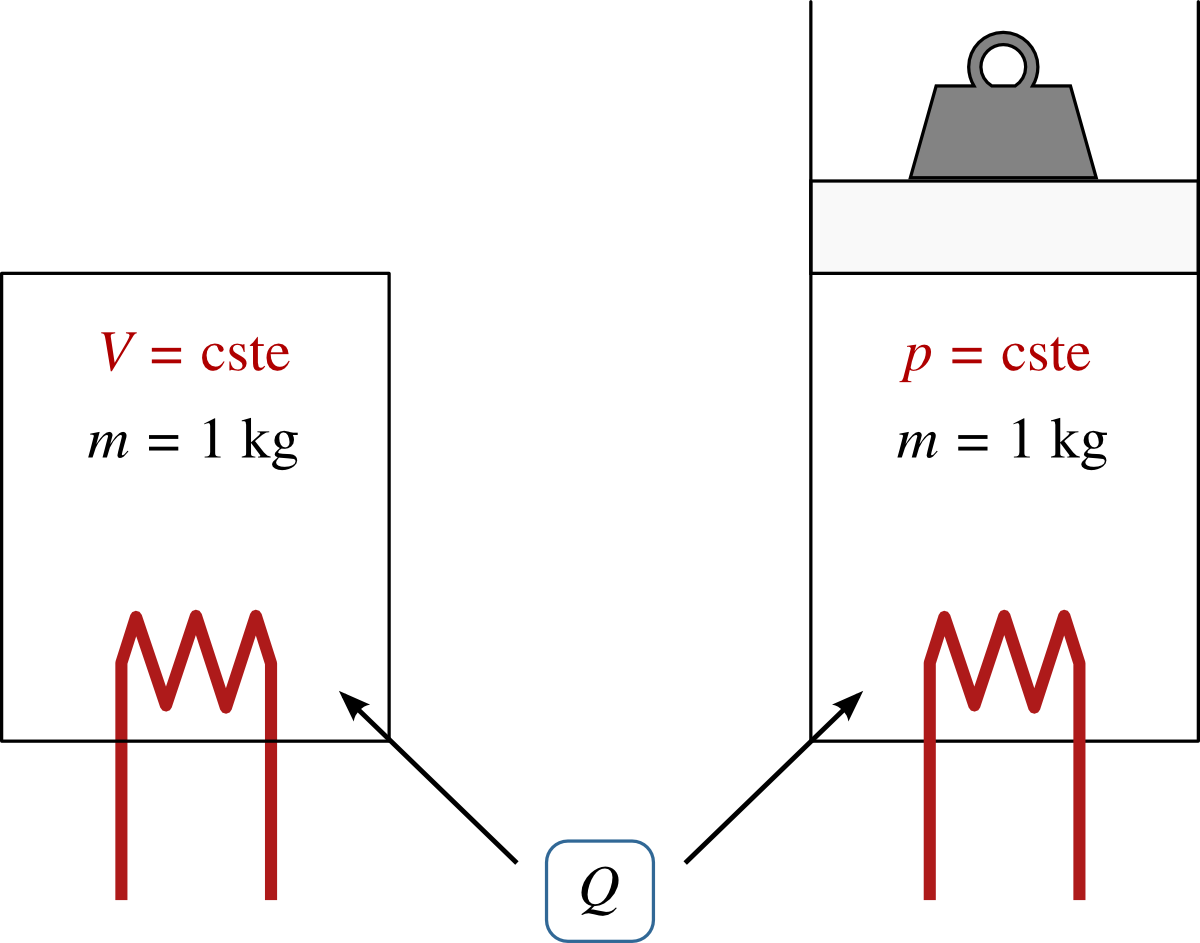
\includegraphics[width=10cm]{images/difference_capacites_calorifiques.png}
			\end{center}
			\supercaption{Deux quantités identiques de gaz reçoivent la même quantité de chaleur $Q$ . L’élévation de température sera plus faible à droite à cause du travail effectué sur le piston.}{schéma \cczero \oc}
			\label{fig_expérience_diff_chaleurs_massiques}
		\end{figure}

		Parmi celles-ci, deux valeurs particulières (\cref{fig_cp_et_cv}) nous servent de référence pour décrire le comportement d’un gaz parfait :

		\begin{figure}
			\begin{center}
				\includegraphics[width=9cm]{images/capacites_calorifiques.png}
			\end{center}
			\supercaption{Définitions des chaleurs massiques. À gauche, le volume est fixé et la capacité calorifique massique sera $c_v$. À droite, la pression est constante et la capacité sera $c_p$.}{schéma \cczero \oc}
			\label{fig_cp_et_cv}
		\end{figure}
		
		\begin{description}
			\item[la chaleur massique à volume constant :]$c_v$~, \dontbreakpage
			\item[la chaleur massique à pression constante :]$c_p$~.
		\end{description}

		Ces deux propriétés vont nous servir très bientôt pour quantifier l’énergie dans les gaz. $c_v$ et $c_p$ sont indépendantes de la température dans un gaz parfait. Dans les gaz réels, elles varient avec la température (\cref{fig_valeurs_de_cp_cv_gamma}), mais pour la plupart des applications en ingénierie il est raisonnable d’utiliser des valeurs moyennes. Pour l’air, nous retenons $c_{v\text{(air)}} = \SI{718}{\joule\per\kilogram\per\kelvin}$ et $c_{p\text{(air)}} = \SI{1005}{\joule\per\kilogram\per\kelvin}$.

		\begin{figure}
			\begin{center}
				\includegraphics[width=15cm, inner]{images/valeurs_cp_cv_air.png}
			\end{center}
			\supercaption{Capacité calorifique de l’air en fonction de sa température. On note une variation sensible des valeurs dans la gamme de températures utilisée en ingénierie, que nous négligerons dans le cadre de notre étude de la thermodynamique.}%
				{Données issues du circulaire NBS 564 “Tables of Thermal Properties of Gases” (1955) jusqu’à~\SI{1000}{\kelvin}, calculées selon le modèle de B. G. Kyle in “Chemical and Process Thermodynamics” (1984) ensuite, et publiées par Israel Urieli (\href{http ://www.ohio.edu/mechanical/thermo/}{ohio.edu/mechanical/thermo/})}
		\label{fig_valeurs_de_cp_cv_gamma}
		\end{figure}




	\subsection{Différence des chaleurs massiques}

		Le grand nombre d’équations que nous abordons rend utile, mais pas indispensable, cette courte section. Pour l’ingénieur/e, il n’a d’autre intérêt que de permettre d’alléger l’écriture des relations de la section suivante.

		Observons les quantités d’énergie en jeu dans l’expérience décrite en \cref{fig_cp_et_cv}. Nous fournissons à chaque corps une quantité de chaleur différente pour obtenir la même variation de température. La différence entre les deux quantités de chaleur requises provient du fait que le gaz à pression constante (à droite) a fourni un travail pendant l’évolution.

		Quelle est la différence entre les chaleurs massiques de chacun des gaz ? Dans chacun des deux cas, nous avons $q_{1 \to 2} + w_{1 \to 2} = \Delta u$ (\ref{eq_premier_principe_sf_min}). Pour le corps A à gauche, comme aucun travail n’est effectué et que l’évolution est à volume constant, nous pouvons écrire :
			\begin{equation}
				\left\{
					\begin{array}{rl}
						q_\A 		& = c_v \ \Delta T \\
						\Delta u 			& = q_\A
					\end{array} \right.
			\label{eq_sectionmathschiante_0}
			\end{equation}

		Pour le corps B à droite, comme la pression $p_\text{cste}$ est constante, nous pouvons écrire :
			\begin{equation}
				\left\{
					\begin{array}{rl}
						q_\B 		& = c_p \ \Delta T \\
						\Delta u 	& = q_\B + (-p_\text{cste} \ \Delta v)
					\end{array} \right.
			\label{eq_sectionmathschiante_1}
			\end{equation}


		En combinant les deux systèmes~\ref{eq_sectionmathschiante_0} et~\ref{eq_sectionmathschiante_1}%
			\footnote{En étant véritablement rigoureux, pour affirmer que $\Delta u_A$ et $\Delta u_B$ sont égaux, il nous faudrait attendre l’\cref{eq_principe_de_joule} qui arrive à la section suivante.}%
		, nous obtenons
		\begin{equation}
			c_v \ \Delta T = c_p \ \Delta T - p_\text{cste} \ \Delta v
		\end{equation}

		qui stipule simplement que la différence entre les deux chaleurs fournies est retrouvée dans le travail fourni par le gaz de droite.

		Une brève manipulation amène :
		\begin{IEEEeqnarray}{rCl}
			(c_p - c_v) \Delta T 	& = & p_\text{cste} \ \Delta v	\nonumber \\
			(c_p - c_v) 				& = & \frac{pv_2 - pv_1}{\Delta T} = \frac{R T_2 - R T_1}{\Delta T} = \frac{R \ \Delta T}{\Delta T}	\nonumber \\
			c_p - c_v 					& = & R
		\label{eq_sectionmathschiante_2}
		\end{IEEEeqnarray}

		Cette expression a pour seul intérêt de nous permettre de simplifier l’\cref{eq_h_fonction_de_T} que nous allons écrire plus bas.


	\subsection{Quotient des chaleurs massiques}

		Le ratio des chaleurs massiques à pression et à volume constants est nommé $\gamma $. Ainsi :
		\begin{equation}
			\gamma \equiv \frac{c_p}{c_v}
			\label{def_gamma}
		\end{equation}

		En retournant à la \cref{fig_cp_et_cv} il apparaît rapidement que $c_p$ doit être supérieur à $c_v$ ; ainsi $\gamma$ est toujours supérieur à~\num{1}. Nous retenons $\gamma_\text{air} = \num{1,4}$.
		
		

\section{Énergie et température}

	\subsection{Contexte historique}
	
		\onlyframabook{\thermoquotebegin{O}%handmade citation remontée d’un paragraphe dans le framabook, sinon la mise en page est cassée
			M’étant assuré de ce fait important, que plus un espace est vide, et plus il s’en dégage de la chaleur lorsque l’air extérieur y pénètre, j’ai cherché à déterminer, par des expériences exactes, quelle relation il y avoit entre le calorique absorbé dans l’un des récipiens et celui dégagé dans l’autre, et comment ces variations de température dépendoient de celles de la variation de la densité de l’air.
		\thermoquoteend{Louis Joseph Gay-Lussac, 1807~\cite{gaylussac1807}}{\vspace{1em}}} %handmade vspace
	
		Au tout début du \textsc{xix}\ieme siècle ont lieu les premiers travaux de recherche visant à explorer la notion de température. La communauté scientifique s’intéresse alors beaucoup aux gaz -- on s’aperçoit qu’il y a \emph{deux} manières de faire augmenter leur température : en les chauffant, mais aussi en les comprimant.
		
		\onlyamphibook{\thermoquotebegin{O}%handmade la citation est ici au bon endroit, dans les Amphibooks seulement.
			M’étant assuré de ce fait important, que plus un espace est vide, et plus il s’en dégage de la chaleur lorsque l’air extérieur y pénètre, j’ai cherché à déterminer, par des expériences exactes, quelle relation il y avoit entre le calorique absorbé dans l’un des récipiens et celui dégagé dans l’autre, et comment ces variations de température dépendoient de celles de la variation de la densité de l’air.
		\thermoquoteend{Louis Joseph Gay-Lussac, 1807~\cite{gaylussac1807}}{\vspace{1em}}} %handmade vspace
		
		Le français \wf{Louis Joseph Gay-Lussac} cherche à comprendre pourquoi la température d’un gaz chute lorsqu’il se détend (il cherche en fait, selon les concepts d’alors, à identifier la source du \textit{calorique} et les raisons pour lesquelles il s’écoule). Il s’efforce ainsi de produire des détentes de gaz aussi simples que possible, et d’y mesurer la température. Une trentaine d’années plus tard, l’anglais \wf{James Prescott Joule} reprend et approfondit ces expériences\footnote{Les travaux méticuleux de Joule mèneront à la première expression formelle du premier principe de la thermodynamique, et à la fin de la théorie du \textit{calorique} selon laquelle la chaleur était un fluide très peu dense et invisible. Ils vaudront à son nom de famille l’utilisation que l’on sait aujourd’hui.} ; mais cette fois, en quantifiant la chaleur en tant qu’\textit{équivalence de travail}. Ces expériences avec ballons de gaz et thermomètres sont tout sauf spectaculaires -- mais elles vont jouer un rôle pivot en thermodynamique, parce qu’elles permettent de distinguer pour la première fois chaleur, travail, énergie et température.

	\subsection{La loi de Joule}
	\label{ch_principe_de_joule}

		\thermoquotebegin{O}
			J’ai pris deux ballons à deux tubulures, chacun de douze litres de capacité. A l’une des tubulures de chaque ballon étoit adapté un robinet, et à l’autre un thermomètre à alcool très-sensible, dont les degrés centigrades pouvoient être facilement divisés en centièmes. […] Le vide étant fait dans les deux ballons, et m’étant assuré qu’ils le retenoient exactement, je remplissois l’un d’eux avec le gaz sur lequel je voulois opérer. Environ douze heures après, j’établissois entre eux une communication au moyen d’un tuyau de plomb, et en ouvrant les robinets, le gaz se précipitoit alors dans le ballon vide jusqu’à ce que l’équilibre de pression fût rétablit de part et d’autre. Pendant ce tems, le thermomètre éprouvoit des variations que je notois avec soin.
		\thermoquoteend{Louis Joseph Gay-Lussac, 1807~\cite{gaylussac1807}}{\vspace{-1em}} %handmade vspace
		Dans leur expérience la plus remarquable, Joule et Gay-Lussac cherchent à faire varier la pression et le volume d’un gaz \textit{sans lui transférer de chaleur ou de travail}. Pour cela, ils laissent un gaz comprimé se détendre dans un second récipient vide (\cref{fig_detente_joule}). Le travail effectué est nul, car aucune surface n’a été déplacée – l’évolution est entièrement irréversible. La température est mesurée et… il ne se passe rien ! Joule et Gay-Lussac ne mesurent ni transferts de chaleur, ni variation de température.

		\begin{figure}
			\onlyframabook{\vspace{1.5em}}%handmade pour faire tenir la citation sur le côté
			\begin{center}
				\includegraphics[width=9cm]{images/detente_joule_gay-lussac.png}
			\end{center}
			\supercaption{La \wfd{D\%C3\%A9tente de Joule-Gay-Lussac}{détente de Joule et Gay-Lussac}.\\			
		Un gaz est initialement prisonnier d’un réservoir à gauche ; on le laisse se détendre en ouvrant la vanne (au centre) qui le sépare d’un réservoir entièrement vide à droite.\\		
		Joule et Gay-Lussac s’intéressent aux variations de température mesurées dans chaque réservoir. Plus les propriétés du gaz rapprochent son comportement du modèle des gaz parfaits (\S\ref{ch_pas_gaz_parfait}), plus les variations de température qu’ils mesurent sont faibles, jusqu’à devenir indétectables pour certains gaz simples à haute température.}{schéma \cczero \oc}
			\label{fig_detente_joule}
		\end{figure}

		Joule effectue une multitude d’expériences différentes au cours desquelles il observe que quel que soit le travail fourni, la relation entre énergie interne (qui ne varie qu’avec travail et chaleur) et température reste sensiblement la même --\ et il suggère que pour un gaz parfait, elle reste toujours identique.

		Ce postulat est connu sous le nom de \vocab{loi de Joule} et est posé comme vrai pour tout gaz parfait. On peut le résumer ainsi :

		\begin{trucimportant}
			La température d’un gaz parfait ne varie qu’avec son énergie interne.
		\end{trucimportant}


		\thermoquotebegin{O}
La différence entre les moyennes des expansions et des expériences-témoin étant exactement telle que ce que à quoi nous avons attribué l’effet croissant de la température ambiante dans le dernier cas, nous arrivons à la conclusion qu’\emph{il n’y a pas de changement de température lorsque l’on laisse l’air se détendre d’une façon telle qu’il ne développe pas de puissance mécanique}.
		\thermoquoteend{James Joule, 1845~\cite{joule1845}}{}
		Mathématiquement, nous pouvons l’écrire ainsi :
		\begin{equation}
			u = f(T)
		\end{equation}

		La fonction $f$ peut être évaluée avec une expérience dans laquelle la variation de~$u$ est quantifiée. Par exemple, lors d’une évolution à volume constant $q = \Delta u$ et $q = c_v \ \Delta T$. On peut ainsi affirmer que la fonction $f$ est une simple relation de proportionnalité. L’énergie interne pouvant être arbitrairement posée comme nulle à température nulle ($u = \SI{0}{\joule\per\kilogram}$ lorsque $T = \SI{0}{\kelvin}$), on obtient :
		\begin{equation}
			u = c_v \ T
			\label{eq_principe_de_joule}
		\end{equation}
		\begin{equationterms}
			\item pour tout gaz parfait,
			\item quelle que soit l’évolution (réversible ou non),
			\item où \tab $u$ 	\tab est l’énergie interne spécifique (\si{\joule\per\kilogram}) ;
			\item 	\tab $T$ 	\tab est la température (\si{\kelvin}) ;
			\item et \tab $c_v$ 	\tab est la capacité calorifique massique à volume constant (\si{\joule\per\kilogram\per\kelvin}).
		\end{equationterms}

		Pour une masse $m$ de gaz parfait, on a bien sûr :
		\begin{equation}
			U = m \ c_v \ T
			\label{eq_principe_de_joule_m}
		\end{equation}

		Tant que notre fluide se comporte comme un gaz parfait, cette relation~\ref{eq_principe_de_joule} reste vraie. Elle fonctionne pendant toute évolution, réversible ou non, et quelles que soient les contraintes de volume, de pression ou de température.

		Par contre, il faut bien noter que cette \cref{eq_principe_de_joule}, qui découle de la loi de Joule, n’est pas du tout valable dans le cas des liquides et vapeurs. On peut, par exemple, ajouter de l’énergie à une masse d’eau bouillante, sans que sa température n’augmente. Nous étudierons les liquides et vapeurs dans le \courscinqshort.
		
		\begin{anexample}
			La chaleur massique à volume constant de l’air est mesurée à $c_{v\text{(air)}} = \SI{718}{\joule\per\kilogram\per\kelvin}$.\\
			On prend une masse de~\SI{0,5}{\kilogram} d’air à~\SI{20}{\degreeCelsius} et on lui transfère \SI{+15}{\kilo\joule} sous forme de chaleur et~\SI{-10}{\kilo\joule} sous forme de travail. Quelle est sa température finale ?
				\begin{answer}
					Nous savons que l’énergie a varié avec les transferts : $\Delta U = W_\fromatob + Q_\fromatob = m \ c_v \ \Delta T$. Ainsi, la température a varié en proportion : $T_\B = T_\A + \frac{\Delta U}{m \ c_v} = T_\A + \frac{W_\fromatob + Q_\fromatob}{m \ c_v} = \num{20} + \frac{\num{-10e3} + (\num{+15e3})}{\num{0,5} \times \num{718}} = \SI{33,92}{\degreeCelsius}$
				\end{answer}
					\begin{remark}Sacré James ! Il nous suffit de quantifier les variations d’énergie pour connaître la température, et vice-versa.\end{remark}
					\begin{remark}Ici les températures ne sont qu’additionnées et une conversion en \si{kelvins} n’aurait pas modifié le résultat. En cas de doute, il vaut mieux ne pas prendre ce raccourci. \end{remark}
		\end{anexample}



	\subsection{Enthalpie d’un gaz parfait}

		Parce que nous venons de lier l’énergie interne $u$ à la température et que le produit $p v$ dépend lui aussi de la température, nous pouvons désormais facilement exprimer l’enthalpie $h$ d’un gaz parfait en fonction de la température uniquement.

		En effet, nous avons $h \equiv u + p v$ (\ref{def_enthalpie}) ; avec une rapide insertion des équations~\ref{eq_pv=RT} et~\ref{eq_principe_de_joule} nous pouvons écrire, pour tout gaz parfait :
			\begin{equation}
				h = u + p v = c_v T + R T = (c_v + R) \ T
				\label{eq_h_fonction_de_T}
			\end{equation}

		Avec l’\cref{eq_sectionmathschiante_2} que nous avons développée plus haut, nous pouvons simplifier cette expression pour obtenir :
			\begin{equation}
				h = c_p \ T
				\label{eq_h=cpT}
			\end{equation}
			\begin{equationterms}
				\item Pour tout gaz parfait,
				\item quelle que soit l’évolution (réversible ou non),
				\item où \tab $h$ 	\tab est l’enthalpie spécifique (\si{\joule\per\kilogram}) ;
				\item 	\tab $T$ 	\tab est la température (\si{\kelvin}) ;
				\item et \tab $c_p$ 	\tab est la capacité calorifique massique à pression constante (\si{\joule\per\kilogram\per\kelvin}).
			\end{equationterms}
		
		
		\begin{anexample}
			La chaleur massique à pression constante de l’air est mesurée à $c_{p\text{(air)}} = \SI{1005}{\joule\per\kilogram\per\kelvin}$.\\
			Un débit de~\SI{2}{\kilogram\per\second} d’air passe dans un compresseur, où sa température augmente de~\SI{150}{\degreeCelsius}. Quelle est la puissance consommée par le compresseur ?
				\begin{answer}
					Nous savons que l’énergie est directement proportionnelle à la variation de température. Avec les équations \ref{eq_grande_sfee_deltas_h} et \ref{eq_h=cpT}, nous obtenons : $\dot W_\fromatob + \dot Q_\fromatob = \dot m \ \Delta h = \dot m \ c_p \ \Delta T = 2 \times \num{1005} \times (\num{+150}) = \SI{+301,5}{\kilo\watt}$.
				\end{answer}
					\begin{remark}Avec un gaz parfait, un simple thermomètre suffit pour quantifier l’énergie…\end{remark}
					\begin{remark}…mais pas pour différencier travail et chaleur. Ici nous ne pouvons pas séparer $\dot W_\fromatob$ de $\dot Q_\fromatob$. Nous ne pouvons pas non plus prédire l’état du gaz à la sortie, c’est à dire sa pression $p$ et son volume spécifique $v$ (seulement leur multiple). Pour cela, il faudrait une description précise de ce qui se passe entre l’entrée et la sortie.\end{remark}
		\end{anexample}


	\subsection{Interlude : Que retenir du gaz parfait jusqu’ici ?}

		Le gaz parfait est un modèle pour quantifier la température d’un gaz. Selon ce modèle, les trois principales formes d’énergie que nous avons utilisées jusqu’à présent —~l’énergie interne~$u$, l’enthalpie spécifique~$h$ et le terme~$p v$~— sont directement proportionnelles à la température~$T$ :
		\begin{IEEEeqnarray*}{rClC}
			u 	& = & c_v T 	& \qquad (\si{\joule\per\kilogram})	\\
			h 	& = & c_p T	& \qquad (\si{\joule\per\kilogram}) 	\\
			p v 	& = & R T 	& \qquad (\si{\joule\per\kilogram})
		\end{IEEEeqnarray*}

		Si l’on mesure la température absolue d’un gaz, alors on peut quantifier immédiatement ces trois formes d’énergie.




\section{Transformations élémentaires réversibles}
\label{ch_gp_evolutions_elementaires}

	Nous nous proposons ici de calculer les propriétés d’un gaz parfait, ainsi que les transferts d’énergie en jeu, lorsqu’on le comprime ou détend selon des contraintes entièrement arbitraires de volume, pression ou température.


	\subsection{À quoi sert cette section de chapitre ?}
	\label{ch_gp_evolutions_elementaires_aquoisert}

		Les évolutions de gaz que nous étudions ici sont très hypothétiques et pas nécessairement passionnantes, mais elles méritent l’attention de l’étudiant/e pour deux raisons :

		\begin{enumerate}
			\item Le comportement d’un gaz, même avec le modèle du gaz parfait, est intrinsèquement complexe. Ces évolutions élémentaires font figure de gymnastique et permettent d’apprendre à le décrire étape par étape ;
			\item Ces évolutions élémentaires sont des outils conceptuels que nous assemblerons plus tard, d’abord pour quantifier les limites théoriques des machines (au \coursseptshort), puis pour décrire le comportement des gaz à l’intérieur des machines réelles (au \coursdixshort).
		\end{enumerate}


	\subsection{Évolutions à pression constante}
	\label{ch_gp_isobares}

		Il est possible de chauffer ou refroidir un gaz en maintenant sa pression constante (\cref{fig_gp_pression_constante}). Une évolution à pression constante est dite \vocab{isobare}. Pour générer une telle transformation, nous pouvons :
		
		\begin{itemize}
			\item avec un système fermé, chauffer ou refroidir le gaz en maintenant une force constante sur les parois ;
			\item avec un système ouvert, chauffer ou refroidir le gaz en le laissant simplement s’écouler dans un conduit, sans pièce mobile. C’est le cas par exemple dans la chambre de combustion d’un turboréacteur.
		\end{itemize}

		\begin{figure}
			\begin{center}
				\includegraphics[width=8cm]{images/pression_constante.png}
			\end{center}
			\supercaption{Évolution à pression constante (isobare) d’un gaz parfait. En système fermé (à gauche), le piston exerce une force constante tout au long de l’évolution. En système ouvert (à droite), aucun travail n’est effectué.}{\cczero \oc}
			\label{fig_gp_pression_constante}
		\end{figure}
		
		\begin{figure}
			\begin{center}
				\includegraphics[width=\pvdiagramwidth]{images/pv_isobare.png}
			\end{center}
			\supercaption{Réchauffement à pression constante d’un gaz parfait, représenté sur un diagramme pression-volume.}{\cczero \oc}
			\label{fig_gp_pression_constante_pv}
		\end{figure}		

		Lorsque la pression est constante, les propriétés du gaz varient selon la relation
		\begin{equation}
			\frac{T}{v} = \text{constante}
		\end{equation}
		
		
		En système fermé, nous avons $q_{1\to2} + w_{1\to2} = \Delta u$ (\ref{eq_premier_principe_sf_min}) et, si l’évolution est réversible, la chaleur et le travail peuvent être facilement reliés à la température :
		\begin{IEEEeqnarray}{rCl}
			w_{1\to2} 	& = & - \int _1^2 p \diff v = -p_\text{cste} \int _1^2 \diff v = -p_\text{cste} \ \Delta v	\nonumber \\
			w_{1 \to 2} 	& = & - R \ \Delta T
		\end{IEEEeqnarray}
		\begin{equationterms}
			\item lors d’une évolution réversible à pression constante $p_\text{cste}$, en système fermé.
		\end{equationterms}

		On remarque que le travail est de signe opposé à la variation de température.
		
		La chaleur peut être quantifiée aisément :
		\begin{IEEEeqnarray}{rCl}
			q_{1\to2} 	& = & \Delta u - w_{1\to2} = \Delta u + p_\text{cste} \ \Delta v = \Delta h \nonumber \\
			q_{1 \to 2} 	& = & c_p \ \Delta T \label{eq_q_gp_sf_isobare}
		\end{IEEEeqnarray}
		\begin{equationterms}
			\item lors d’une évolution réversible à pression constante, en système fermé.
		\end{equationterms}

		
		Lorsque l’évolution se fait en système ouvert, nous avons $q_{1\to2} + w_{1\to2} = \Delta h$ (\ref{eq_petite_sfee_deltas_h}), et, si l’évolution est réversible, la chaleur et le travail se quantifient sans peine :		
		\begin{IEEEeqnarray}{rCl}
			w_{1\to2} 	& = & \int _1^2 v \diff p \nonumber \\
			w_{1\to2} 	& = & 0
		\end{IEEEeqnarray}
		\begin{equationterms}
			\item lors d’une évolution réversible à pression constante, en système ouvert.
		\end{equationterms}

		Le travail est bien sûr nul, puisqu’aucune pièce mobile n’est présente pour extraire de l’énergie mécanique du gaz.

		La chaleur est alors responsable de l’entièreté de la variation de température :
		\begin{IEEEeqnarray}{rCl}
			q_{1\to2} 	& = & \Delta h - w_{1\to2} = \Delta h \nonumber \\
			q_{1 \to 2} 	& = & c_p \ \Delta T \label{eq_q_gp_so_isobare}
		\end{IEEEeqnarray}
		\begin{equationterms}
			\item lors d’une évolution réversible à pression constante, en système ouvert.
		\end{equationterms}

		\begin{anexample}
			Pour l’air, on mesure $c_{p\text{(air)}} = \SI{1005}{\joule\per\kilogram\per\kelvin}$, $c_{v\text{(air)}} = \SI{718}{\joule\per\kilogram\per\kelvin}$, $R_\text{air} = \SI{287}{\joule\per\kilogram\per\kelvin}$.
			Combien faut-il d’énergie pour chauffer l’air dans un appartement de~\SI{30}{\metre\squared} depuis \SI{10}{\degreeCelsius} jusqu’à \SI{20}{\degreeCelsius} ?
				\begin{answer}
					Le réchauffement se fera vraisemblablement à pression constante (à moins que l’appartement ne soit fermé hermétiquement, la pression sera partout atmosphérique et l’air «~fuira~» sous les portes). Nous supposons une pression de~\SI{1}{\bar} et une hauteur de plafond de~\SI{2,5}{\metre}. Nous utilisons un système fermé englobant tout l’air réchauffé.
					
					Nous avons un volume de~\SI{75}{\metre\cubed}, ce qui mène la masse totale d’air à $m_\A = \frac{p_\A \ V_\A}{R \ T_\A} = \frac{\num{1e5} \times \num{75}}{\num{287} \times (\num{10} + \num{273,15})} = \SI{92,29}{\kilogram}$.\\
					La chaleur nécessaire pour chauffer cette quantité d’air à pression constante est quantifiable avec l’\cref{eq_q_gp_sf_isobare} : $Q_\fromatob = m \ c_p \ \Delta T = \num{93,29} \times \num{1005} \times (\num{20} - \num{10}) = \SI{+9,28e5}{\joule} = \SI{+928}{\kilo\joule}$.
				\end{answer}
					\begin{remark}Ce résultat représente le transfert final \emph{net} de chaleur vers l’air (incluant les pertes vers les murs et les fenêtres, ainsi que les transferts qui les compensent).\end{remark}
					\begin{remark}À l’inverse, un refroidissement provoquerait l’arrivée d’air extérieur, dont il faudrait tenir compte dans le calcul de la masse.\end{remark}
		\end{anexample}

	\subsection{Évolutions à volume constant}
	\label{ch_gp_isochores}

		Il est possible de chauffer ou refroidir un gaz en maintenant son volume constant (\cref{fig_gp_volume_constant}). Une évolution à volume constant est dite \vocab{isochore}.
			
		\begin{itemize}
			\item Avec un système fermé, nous pouvons chauffer ou refroidir un gaz dans un réservoir fixe et fermé. C’est le cas par exemple pendant la phase de combustion («~explosion~») dans un moteur à essence.
			\item Avec un système ouvert, la manipulation est plus complexe. Nous devons compresser le gaz pendant qu’on le réchauffe pour éviter que son volume n’augmente ; À l’inverse, pendant un refroidissement, il faut le détendre pour éviter que son volume ne baisse. Cette manipulation n’a pas d’application pratique courante.
		\end{itemize}	
		
		\begin{figure}
			\begin{center}
				\includegraphics[width=8cm]{images/volume_constant.png}
			\end{center}
			\supercaption{Évolution à volume constant (isochore) d’un gaz parfait. En système fermé (à gauche), le volume est bloqué et aucun travail n’est effectué. En système ouvert (à droite), on doit comprimer le gaz pendant qu’on le chauffe et le détendre pendant qu’on le refroidit, pour pouvoir maintenir le volume spécifique constant.}{\cczero \oc}
			\label{fig_gp_volume_constant}
		\end{figure}
		
		\begin{figure}
			\begin{center}
				\includegraphics[width=\pvdiagramwidth]{images/pv_isochore.png}
			\end{center}
			\supercaption{Refroidissement à volume constant d’un gaz parfait, représenté sur un diagramme pression-volume.}{\cczero \oc}
			\label{fig_gp_volume_constant_pv}
		\end{figure}		

		Lorsque le volume spécifique d’un gaz parfait est constant, ses propriétés varient selon la relation
		\begin{equation}
			\frac{T}{p} = \text{constante} \label{eq_gp_isochore}
		\end{equation}
		
		En système fermé, nous avons $q_{1\to2} + w_{1\to2} = \Delta u$ et, si l’évolution est réversible, la chaleur et le travail peuvent être facilement reliés à la température.

		Le volume ne variant pas, le travail est bien sûr nul :
		\begin{IEEEeqnarray}{rCl}
			w_{1\to2} 	& = & - \int _1^2 p \diff v	\nonumber \\
			w_{1\to2} 	& = & 0 \label{eq_w_gp_sf_isochore}
		\end{IEEEeqnarray}
		\begin{equationterms}
			\item lors d’une évolution réversible à volume constant, en système fermé.
		\end{equationterms}

		La chaleur peut être quantifiée aisément :
		\begin{IEEEeqnarray}{rCl}
			q_{1\to2} 	& = & \Delta u - w_{1\to2} = \Delta u \nonumber \\
			q_{1\to2} 	& = & c_v \ \Delta T \label{eq_q_gp_sf_isochore}
		\end{IEEEeqnarray}
		\begin{equationterms}
			\item lors d’une évolution réversible à volume constant, en système fermé.
		\end{equationterms}

		
		Lorsque l’évolution se fait en système ouvert, nous avons $q_{1\to2} + w_{1\to2} = \Delta h$ et, si l’évolution est réversible, la chaleur et le travail peuvent être quantifiés, bien qu’avec un peu plus de difficulté :
		\begin{IEEEeqnarray}{rCl}
			w_{1\to2} 	& = & \int _1^2 v \diff p = v_\text{cste} \int_1^2 \diff p = v_\text{cste} \int_1^2 \frac{R}{v_\text{cste}} \diff T = R \int_1^2 \diff T \nonumber \\
			w_{1\to2} 	& = & R \ \Delta T
		\end{IEEEeqnarray}
		\begin{equationterms}
			\item lors d’une évolution réversible à volume constant, en système ouvert.
		\end{equationterms}

		On peut alors quantifier facilement la chaleur à fournir :
		\begin{IEEEeqnarray}{rCl}
			q_{1\to2} 	& = & \Delta h - w_{1\to2} = c_p \ \Delta T - R \ \Delta T \nonumber \\
			q_{1\to2} 	& = & c_v \ \Delta T
		\end{IEEEeqnarray}
		\begin{equationterms}
			\item lors d’une évolution réversible à volume constant, en système ouvert.
		\end{equationterms}

		\begin{anexample}
			Pour l’air, on mesure $c_{p\text{(air)}} = \SI{1005}{\joule\per\kilogram\per\kelvin}$, $c_{v\text{(air)}} = \SI{718}{\joule\per\kilogram\per\kelvin}$, $R_\text{air} = \SI{287}{\joule\per\kilogram\per\kelvin}$.\\
			Dans un cylindre de moteur à essence, de l’air se trouve à pression de~\SI{17}{\bar} avec une masse volumique de~\SI{9,4}{\kilogram\per\metre\cubed}. La combustion du carburant (si rapide que le volume n’a pas le temps de varier) se traduit par l’apport de~\SI{1450}{\kilo\joule\per\kilogram} de chaleur. Quelles valeurs atteignent la température et la pression ?
				\begin{answer}
					Au départ, la température est $T_\A = \frac{p_\A v_\A}{R} = \frac{p_\A}{\rho_A R} = \frac{\num{17e5}}{\num{9,4} \times \num{287}} = \SI{630,1}{\kelvin} = \SI{357}{\degreeCelsius}$.\\
					Nous utilisons un système fermé constitué par la masse d’air. Le volume ne variant pas, le travail est nul (\ref{eq_w_gp_sf_isochore}) et c’est la chaleur qui fait varier l’énergie interne (\ref{eq_q_gp_sf_isochore}) : $q_\fromatob = \Delta u - w_\fromatob = \Delta u = c_v \ \Delta T$ ; ainsi $T_\B = T_\A + \frac{q_\fromatob}{c_v} = \num{630,1} + \frac{\num{1450e3}}{\num{718}} = \SI{2649,6}{\kelvin} = \SI{2376,5}{\degreeCelsius}$.\\
					La pression finale s’obtient en comparant la condition finale et la condition initiale (\ref{eq_gp_isochore}) : $\frac{R T_\A}{p_\A} = v_\A = v_\B = \frac{R T_\B}{p_\B} $ ; ainsi $p_\B = \frac{T_\B}{T_\A} p_\A = \frac{\num{2649,6}}{\num{630,1}} \times \num{17e5} = \SI{7,148e6}{\pascal} = \SI{71,5}{\bar}$.
						\begin{remark}Attention à bien compter les températures en \si{kelvins} dans les fractions.\end{remark}
						\begin{remark}La température maximale, supérieure à~\SI{2300}{\degreeCelsius}, dépasse la température de fonte de la plupart des métaux. Dans un moteur à essence, cette température n’est atteinte que sporadiquement, à chaque combustion.\end{remark}
						\begin{remark}Les données de cet exemple imitent celles de l’exercice \ref{exo_cycle_moteur_essence}. Cette fois, nous savons prédire les conditions finales sans devoir faire de mesure.\end{remark}
				\end{answer}
		\end{anexample}

	\subsection{Évolutions à température constante}
	\label{ch_gp_isothermes}
	
		\thermoquotebegin{O}
			Il est facile d’imaginer une petite quantité de combustible gazeux ou liquide, ou bien de la poussière de charbon, que l’on insèrerait dans un volume d’air comprimé et très chaud, et qui brûlerait suite à un allumage séparé ou spontané. Le piston est chassé en même temps de sorte qu’aucune augmentation de température n’ait lieu, car la chaleur développée par chaque particule de combustible est instanément absorbée par le refroidissement dû à l’expansion. De cette façon l’ensemble de la chaleur est transformée en travail.
		\thermoquoteend{Rudolf Diesel, 1893}{\textit{Theorie und Konstruktion eines rationellen Wärmemotors zum Ersatz der Dampfmaschinen und der heute bekannten Verbrennungsmotoren}~\mbox{\cite{diesel1893,diesel1893en}}\vspace{5em}} %handmade vspace
		Il est possible de chauffer ou refroidir un gaz en maintenant sa température constante (\cref{fig_gp_température_constante}). Une évolution à température constante est dite \vocab{isotherme}.
		
		\begin{figure}
			\begin{center}
				\includegraphics[width=8cm]{images/temperature_constante.png}
			\end{center}
			\supercaption{Évolution à température constante (isotherme) d’un gaz parfait. En système fermé (à gauche), on laisse travailler le gaz sur un piston pendant qu’on le chauffe, et à l’inverse, on lui fournit du travail lorsqu’on le refroidit. En système ouvert (à droite), les mêmes manipulations sont effectuées en flux continu.}{\cczero \oc}
			\label{fig_gp_température_constante}
		\end{figure}
		
		\begin{figure}
			\begin{center}
				\includegraphics[width=\pvdiagramwidth]{images/pv_isotherme.png}
			\end{center}
			\supercaption{Détente (réchauffement) à température constante d’un gaz parfait, représenté sur un diagramme pression-volume.}{\cczero \oc}
			\label{fig_gp_température_constante_pv}
		\end{figure}		

		Pour un gaz parfait, une évolution à température constante se fait toujours à énergie constante. Pour chaque joule de chaleur que l’on fournit au gaz, il faut lui prendre un joule sous forme de travail ; inversement chaque prélèvement de chaleur doit être compensé par un apport égal de travail.
		
		En pratique, cette complexité fait que les transferts de chaleur isothermes sont rarement utilisés dans l’industrie. Ils revêtent par contre une importance théorique capitale, que nous étudierons au \courssept.
		
		Lorsque la température d’un gaz parfait reste constante, ses propriétés varient selon la relation
		\begin{equation}
			p \ v = \text{constante}
			\label{eq_gp_isotherme}
		\end{equation}
		

		En système fermé, nous avons $q_{1\to2} + w_{1\to2} = \Delta u$, et, si l’évolution est réversible, la chaleur et le travail peuvent être reliés aux propriétés du gaz, non sans une certaine difficulté toutefois.
		\begin{IEEEeqnarray}{rCl}
			w_{1\to2} 	& = & - \int _1^2 p \diff v = - \int \frac{R \ T_\text{cste}}{v} \diff v = - R \ T_\text{cste} \int_1^2 \frac{1}{v} \diff v = - R \ T_\text{cste} [\ln v]_{v_1}^{v_2} \nonumber \\
			w_{1\to2} 	& = & R \ T_\text{cste} \ln \left(\frac{v_1}{v_2}\right)
			\label{eq_gp_travail_isotherme_sf1}
		\end{IEEEeqnarray}
		\begin{equationterms}
			\item lors d’une évolution réversible à température constante, en système fermé.
		\end{equationterms}

		\thermoquotebegin{O}
			\emph{Lorsqu’un gaz varie de volume sans changer de température, les quantités de chaleur absorbées ou dégagées par ce gaz sont en progression arithmétique, si les accroissemens ou les réductions de volume se trouvent être en progression géométrique.}
			Lorsque l’on comprime un litre d’air maintenu à la température 10° et qu’on le réduit à 1/2 litre, il se dégage une certaine quantité de chaleur. Cette quantité se trouvera toujours la même si l’on réduit de nouveau le volume de 1/2 litre à de 1/4 de litre, de 1/4 de litre à 1/8, ainsi de suite.
		\thermoquoteend{Sadi Carnot, 1824~\cite{carnot1824}}{}
		On peut aussi exprimer le travail en fonction de la pression, puisqu’avec l’\cref{eq_gp_isotherme} on~a :
		\begin{equation*}
			\frac{v_1}{v_2} = \frac{p_2}{p_1}
		\end{equation*}
		ainsi :
		\begin{equation}
			w_{1\to2} 	 = R \ T_\text{cste} \ln \left(\frac{p_2}{p_1}\right)
			\label{eq_gp_travail_isotherme_sf2}
		\end{equation}
		\begin{equationterms}
			\item lors d’une évolution réversible à température constante, en système fermé.
		\end{equationterms}

		La chaleur peut être quantifiée aisément. En effet, l’énergie interne ne varie pas :
		\begin{IEEEeqnarray}{rCl}
			q_{1\to2} 	& = & \Delta u - w_{1\to2} = 0 - w_{1\to2} \nonumber \\
			q_{1\to2} 	& = & -w_{1\to2}
			\label{eq_gp_chaleur_isotherme_sf}
		\end{IEEEeqnarray}
		\begin{equationterms}
			\item lors d’une évolution réversible à température constante, en système fermé.
		\end{equationterms}

		
		Lorsque l’évolution se fait en système ouvert, nous avons $q_{1\to2} + w_{1\to2} = \Delta h$ et, si l’évolution est réversible, la chaleur et le travail peuvent être quantifiés de la même façon :
		\begin{IEEEeqnarray}{rCl}
			w_{1\to2} 	& = & \int _1^2 v \diff p = \int_1^2 \frac{R \ T_\text{cste}}{p} \diff p = R \ T_\text{cste} \int_1^2 \frac{1}{p} \diff p = R \ T_\text{cste} [\ln v]_{p_1}^{p_2} \nonumber \\
			w_{1\to2} 	& = & R \ T_\text{cste} \ln \left(\frac{p_2}{p_1}\right) = R \ T_\text{cste} \ln \left(\frac{v_1}{v_2}\right) \label{eq_travail_température_constante_rep}
		\end{IEEEeqnarray}
		\begin{equationterms}
			\item lors d’une évolution réversible à température constante, en système ouvert.
		\end{equationterms}
		
		Cette relation, identique à l’\cref{eq_gp_travail_isotherme_sf2}, n’aura pas surpris l’étudiant/e perspicace, puisque la relation $p v = \text{cste.}$ assure que pour deux points donnés en \cref{fig_gp_température_constante_pv}, l’aire sous la courbe est toujours égale à l’aire à gauche de la courbe.

		La chaleur à fournir se quantifie bien sûr sans peine :
		\begin{IEEEeqnarray}{rCl}
			q_{1\to2} 	& = & \Delta h - w_{1\to2} = 0 - w_{1\to2} \nonumber \\
			q_{1\to2} 	& = & - w_{1\to2}
		\end{IEEEeqnarray}
		\begin{equationterms}
			\item lors d’une évolution réversible à température constante, en système ouvert.
		\end{equationterms}

		\begin{anexample}
			Pour l’air, on mesure $c_{p\text{(air)}} = \SI{1005}{\joule\per\kilogram\per\kelvin}$, $c_{v\text{(air)}} = \SI{718}{\joule\per\kilogram\per\kelvin}$, $R_\text{air} = \SI{287}{\joule\per\kilogram\per\kelvin}$.\\
			Une masse de~\SI{2,5}{\kilogram} d’air dans un réservoir est à pression de~\SI{2}{\bar} et température de~\SI{800}{\degreeCelsius}. On souhaite lui fournir \SI{100}{\kilo\joule} de chaleur sans modifier sa température. Quel doit être le transfert de travail ? Quels seront le volume et la pression au final ?
			\begin{answer}
				Le travail est facile à déterminer : $W_\fromatob + Q_\fromatob = \Delta U = 0$ ici car la température ne varie pas. Ainsi $W_\fromatob = - Q_\fromatob = \SI{-100}{\kilo\joule}$ (le gaz doit dépenser autant de travail qu’il reçoit de chaleur).\\
				Les propriétés finales sont obtenues grâce à l’\cref{eq_gp_travail_isotherme_sf1} :
						\begin{IEEEeqnarray*}{rCl}
							w_\fromatob 	& = & R \ T_\text{cste} \ln \left(\frac{v_\A}{v_\B}\right) = R \ T_\text{cste} \ln \left(\frac{V_\A}{V_\B}\right)\\
							\frac{V_\A}{V_\B} & = & \exp \left[\frac{w_\fromatob}{R \ T_\text{cste}}\right] = \exp \left[\frac{W_\fromatob}{m \ R \ T_\text{cste}}\right]\\
							 &=& \exp \left[\frac{\num{-100e3}}{\num{2,5} \times 287 \times (\num{800} + \num{273,15})}\right] = \num{0,878207}
						\end{IEEEeqnarray*}
				Et comme $V_\A = \frac{R \ T_\A}{p_\A} = \frac{\num{287} \times (\num{800} + \num{273,15})}{\num{2e5}} = \SI{1,54}{\metre\cubed}$, nous obtenons un volume final $V_\B = \frac{V_\A}{\num{0,878207}} = \SI{1,715}{\metre\cubed}$.\\
				La pression finale, enfin, s’obtient en comparant l’état final et l’état initial : $p_\A V_\A = m \ R \ T_\A = m \ R \ T_\B = p_\B V_\B$ (ou avec l’\cref{eq_gp_travail_isotherme_sf2}) : $p_\B = p_\A \frac{V_\A}{V_\B} = \num{2e5} \times \num{0,878207} = \SI{1,786e5}{\pascal} = \SI{1,786}{\bar}$.
			\end{answer}
				\begin{remark}Le volume augmente et la pression diminue, puisque le gaz travaille en se détendant et en recevant de la chaleur.\end{remark}
				\begin{remark}Il est difficile de cacher que ce type d’évolution est rarement utilisé en pratique, mais il nous servira pour élaborer un prodigieux thermomètre-moteur-réfrigérateur absolu, au \courssept.\end{remark}
		\end{anexample}



	\subsection{Évolutions adiabatiques réversibles}
	\label{ch_gp_isentropiques}

		Une évolution \vocab{adiabatique} est une évolution au cours de laquelle il n’y a aucun transfert de chaleur (\cref{fig_gp_isentropique}). On peut forcer cela en recouvrant le récipient ou le conduit de gaz que l’on compresse ou détend avec une épaisse couche d’isolant thermique.
		
		Attention, même s’il n’y a strictement aucun transfert de chaleur, la température est nécessairement amenée à varier dans une telle évolution, puisque le travail est non-nul. Cette variation de température est d’ailleurs très souvent l’effet escompté, comme nous pourrons le voir au \courssept.
		
		\begin{figure}
			\begin{center}
				\includegraphics[width=8cm]{images/isentropique.png}
			\end{center}
			\supercaption{Évolution adiabatique réversible (isentropique) d’un gaz parfait. En système fermé (à gauche) comme en système ouvert (à droite), l’appareil est parfaitement isolé, de sorte qu’il n’y ait aucun transfert de chaleur, même si la température du gaz varie.}{\cczero \oc}
			\label{fig_gp_isentropique}
		\end{figure}
		
		Une évolution \vocab{adiabatique réversible} est effectuée infiniment lentement. Un piston dans un cylindre devra pour cela être déplacé infiniment lentement, et un compresseur en flux continu devra pour cela être infiniment long. Plus tard, dans le \courshuit, nous appellerons ces transformations \vocab{isentropiques}.

		\begin{figure}
			\begin{center}
				\includegraphics[width=\pvdiagramwidth]{images/pv_isentropique.png}
			\end{center}
			\supercaption{Détente adiabatique réversible d’un gaz parfait, représentée sur un diagramme pression-volume.}{\cczero \oc}
			\label{fig_gp_isentropique_pv}
		\end{figure}

		
		En système fermé, nous avons $q_{1\to2} + w_{1\to2} = \Delta u$ et, si l’évolution est réversible, la chaleur et le travail sont quantifiés sans la moindre difficulté :
		\begin{equation}
			q_{1\to2} = 0
		\end{equation}
		\begin{equationterms}
			\item lors d’une évolution adiabatique réversible, par définition.
		\end{equationterms}
		\begin{IEEEeqnarray}{rCl}
			w_{1\to2} 	& = & \Delta u - q_{1\to2} = \Delta u \nonumber \\
			w_{1 \to 2} 	& = & c_v \ \Delta T
			\label{eq_gp_travail_isentropique_sf}
		\end{IEEEeqnarray}
		\begin{equationterms}
			\item lors d’une évolution adiabatique réversible en système fermé.
		\end{equationterms}

		
		Lorsque l’évolution se fait en système ouvert, nous avons $q_{1\to2} + w_{1\to2} = \Delta h$ et nous pouvons de même écrire :
		\begin{IEEEeqnarray}{rCl}
			q_{1\to2} 	& = & 0 	\\
			w_{1\to2} 	& = & c_p \ \Delta T
			\label{eq_gp_travail_isentropique_so}
		\end{IEEEeqnarray}
		\begin{equationterms}
			\item lors d’une évolution adiabatique réversible, en système ouvert.
		\end{equationterms}

		
		Malheureusement, ces deux équations~\ref{eq_gp_travail_isentropique_sf} et~\ref{eq_gp_travail_isentropique_so} ne sont d’aucune utilité tant que l’on a pas prédit la température $T_2$ à la fin de l’évolution. Or, dans une évolution adiabatique réversible, rien ne reste constant : le volume spécifique, la pression et la température varient tous les trois. Comment quantifier ces propriétés ?
		
		
		Partons d’une évolution adiabatique infiniment courte dans un système fermé. Lorsque l’évolution est réversible, $\diff w = -p \diff v $ et alors :
		\begin{IEEEeqnarray*}{rCl}
			\diff q = \diff u - \diff w 	& = & 0		\nonumber \\
			\diff u + p \diff v				& = & 0
		\end{IEEEeqnarray*}

		Comme $\diff u = c_v \diff T$ pour un gaz parfait et que $p = R T/v $, on peut ré-écrire cette équation ainsi :
		\begin{IEEEeqnarray*}{rCl}
			c_v \diff T + \frac{R T}{v} \diff v								& = & 0	\nonumber \\
			\frac{1}{T} \diff T + \frac{R}{c_v} \frac{1}{v} \diff v 	& = & 0
		\end{IEEEeqnarray*}
	
		En intégrant entre deux états 1 et 2 :
		\begin{IEEEeqnarray}{rCl}
			\ln \left( \frac{T_2}{T_1} \right) + \frac{R}{c_v} \ln \left( \frac{v_2}{v_1} \right) 	& = & 0	\nonumber \\
			\ln \left( \frac{T_2}{T_1} \right) + \ln \left( \frac{v_2}{v_1} \right)^{\frac{R}{c_v}} 	& = & 0	\nonumber \\
			\ln \left( \frac{T_2}{T_1} \right) & = & \ln \left( \frac{v_1}{v_2} \right)^{\frac{R}{c_v}}
			\label{eq_tmp_isentropique}
		\end{IEEEeqnarray}
	
		Et comme $R = c_p-c_v$ (\ref{eq_sectionmathschiante_2}) et $\gamma \equiv c_p/c_v$ (\ref{def_gamma}), on a $\frac{R}{c_v} = \gamma -1$, ce qui permet de reformuler l’\cref{eq_tmp_isentropique} ci-dessus :
		\begin{equation*}
			\left( \frac{T_2}{T_1} \right) = \left(\frac{v_1}{v_2} \right)^{\gamma -1}
		\end{equation*}
	
		Nous avons donc lié température et volume spécifique lorsque l’évolution est adiabatique réversible (privée de transfert de chaleur et infiniment lente).

		Quelques manipulations algébriques, qu’il est laissé à l’étudiant/e le soin de réviser, nous permettent de décliner cette expression en fonction de la pression. On obtient ainsi les trois relations :
		\begin{IEEEeqnarray}{rCl}
			\left( \frac{T_1}{T_2} \right)	& = & \left( \frac{v_2}{v_1} \right)^{\gamma -1}		\label{eq_isentropique_horrible1}\\
			\left( \frac{T_1}{T_2} \right)	& = & \left( \frac{p_1}{p_2} \right)^{\frac{\gamma -1}{\gamma}}	\label{eq_isentropique_horrible2}\\
			\left( \frac{p_1}{p_2} \right)	& = & \left( \frac{v_2}{v_1} \right)^{\gamma}			\label{eq_isentropique_horrible3}
		\end{IEEEeqnarray}
		\begin{equationterms}
			\item pour toute évolution adiabatique réversible.
		\end{equationterms}

		Cette dernière \cref{eq_isentropique_horrible3} équivaut à l’expression :
		\begin{equation}
			p v^{\gamma} = \text{constante}
			\label{eq_isentropique_horrible3bis}
		\end{equation}
		\begin{equationterms}
			\item pour toute évolution adiabatique réversible.
		\end{equationterms}

		Nous disposons donc d’une relation simple entre pression et volume pour un gaz parfait suivant une évolution réversible adiabatique. Remarquons une dernière fois que, même si par définition aucune chaleur n’est transférée, la température varie systématiquement, comme l’indique la relation~\ref{eq_isentropique_horrible1}.
		
		\begin{anexample}
			Pour l’air, on mesure $c_{p\text{(air)}} = \SI{1005}{\joule\per\kilogram\per\kelvin}$, $c_{v\text{(air)}} = \SI{718}{\joule\per\kilogram\per\kelvin}$, $R_\text{air} = \SI{287}{\joule\per\kilogram\per\kelvin}$, et $\gamma_\text{air} = \num{1,4}$.\\
			Un réservoir d’air comprimé de~\SI{50}{\liter} contient de l’air à~\SI{40}{\bar} et~\SI{50}{\degreeCelsius}. L’atmosphère ambiante est à~\SI{1}{\bar}. Quelle est la quantité maximale de travail que l’on peut extraire de l’air comprimé sans lui fournir de chaleur ?
				\begin{answer}
					Le travail maximal sera obtenu si la détente est réversible. Comme nous ne pouvons pas apporter de chaleur, notre meilleure option est donc ici d’effectuer une détente adiabatique réversible depuis \SI{40}{\bar} jusqu’à \SI{1}{\bar}.\\
					Nous voulons calculer la température finale, car c’est elle qui nous donnera la variation d’énergie, donc le travail perdu par le gaz. Des trois intimidantes relations \ref{eq_isentropique_horrible1} à \ref{eq_isentropique_horrible3}, c’est la seconde qui nous intéresse : $\left( \frac{T_\A}{T_\B} \right)	= \left( \frac{p_\A}{p_\B} \right)^{\frac{\gamma -1}{\gamma}}$. Ainsi : $T_\B = T_\A \left( \frac{p_\A}{p_\B} \right)^{-\frac{\gamma -1}{\gamma}} = (\num{50} + \num{273,15}) \left( \frac{40}{1} \right)^{\frac{\num{1,4} -1}{\num{1,4}}} = \SI{112,6}{\kelvin} = \SI{-160,5}{\degreeCelsius}$.\\
					Le travail effectué par le système fermé constitué par le gaz est donc $w_\fromatob = \Delta u - q_\fromatob = c_v \ \Delta T - 0 = \num{718} \times (\num{-160,5} - \num{50}) = \SI{-1,5115e5}{\joule\per\kilogram} = \SI{-151,1}{\kilo\joule\per\kilogram}$.\\
					En calculant la masse $m_\A = \frac{p_\A V_\A}{R \ T_\A} = \frac{\num{40e5} \times \num{0,2}}{287 \times \ (\num{50} + \num{273,15})} = \SI{8,626}{\kilogram}$, nous obtenons $W_\fromatob = m_\A w_\fromatob = \num{8,626} \times \num{-151,1e3} = \SI{-1,3038e6}{\joule} = \SI{-1,304}{\mega\joule}$.
					\begin{remark} Cela représente suffisamment d’énergie pour accélérer sans frottement un véhicule de~\SI{1}{\tonne} jusqu’à une vitesse $C = \left[\frac{\num{1,3038e6}}{\frac{1}{2} \times \num{1000}}\right]^{\num{0,5}} = \SI{51,1}{\metre\per\second} \approx \SI[per-mode = symbol]{180}{\kilo\metre\per\hour}$.\end{remark}
					\begin{remark}La température finale, \SI{-160}{\degreeCelsius} (!), nous rappelle qu’il ne faut pas confondre «~adiabatique~» et «~à température constante~».\end{remark}
					\begin{remark}Les pressions peuvent être laissées en \si{bars} dans les fractions, mais les températures ne peuvent rester en~\si{\degreeCelsius}.\end{remark}
					\begin{remark}La détente correspond au maximum de travail car elle est réversible. Si elle ne l’était pas, alors la température du gaz chuterait moins et le travail serait plus faible (nous aurions toujours $w = c_v \Delta T$). Dans le cas le plus extrême, celui de la détente de Joule et Gay-Lussac (\S\ref{ch_principe_de_joule}), la température resterait fixe à~\SI{50}{\degreeCelsius} et aucun travail ne serait développé.\end{remark}
				\end{answer}
		\end{anexample}

		
	\subsection{Évolutions arbitraires}
	
		Il faut bien garder en tête que l’on peut en pratique faire évoluer les propriétés d’un gaz \emph{de n’importe quelle façon arbitraire} (\cref{fig_gp_pv_coeur}).
		
		\begin{figure}
			\begin{center}
				\includegraphics[width=\pvdiagramwidth]{images/pv_coeur.png}
			\end{center}
			\supercaption{Évolution entièrement arbitraire d’un gaz parfait représentée sur un diagramme pression-volume. Une telle évolution requiert une combinaison complexe de transferts de chaleur et de travail, que l’étudiant/e est invité/e à se représenter.}{\cczero \oc}
			\label{fig_gp_pv_coeur}
		\end{figure}
		
		Nous nous sommes concentrés sur quatre évolutions particulières des gaz parfaits, parce qu’elles jouent chacune un rôle important, pour les physiciens comme pour les ingénieur/es, dans la conception des machines thermiques. Cela ne doit toutefois pas limiter notre façon de «~penser~» un gaz et ses transformations. En contrôlant astucieusement les transferts de chaleur et de travail, nous pouvons bien sûr provoquer n’importe quelle évolution arbitraire.

\atstartofhistorysection
\onlyamphibook{\section[Un peu d’histoire : les questionnements de Lavoisier et Laplace]{Un peu d’histoire :\\ Lavoisier et Laplace s'interrogent sur la nature de la chaleur}}
\onlyframabook{\section[Un peu d’histoire : les questionnements de Lavoisier et Laplace]{Un peu d’histoire : Lavoisier et Laplace s'interrogent sur la nature de la chaleur}}
\label{ch_histoire_lavoisier_laplace_depondt}

\begin{center}\textit{Par Philippe Depondt\\ \begin{small}Université Pierre et Marie Curie, Paris\\ Contribution sous licence \ccbysa\end{small}}\end{center}

	Les débats sur la nature de la chaleur se sont poursuivis jusqu'à la fin du \textsc{xix}\ieme\ siècle avec l'acceptation progressive des théories atomiques. Une étape importante dans cette réflexion est fournie dans le \textit{Mémoire sur la chaleur} (1780~\cite{lavoisierlaplace1780}) de Lavoisier et Laplace :

	\begin{quote} «~Les physiciens sont partagés sur la nature de la chaleur. Plusieurs d’entre eux la regardent comme un fluide répandu dans toute la nature, et dont les corps sont plus ou moins pénétrés, à raison de leur température et de leur disposition particulière à le retenir ; il peut se combiner avec eux, et, dans cet état, il cesse d’agir sur le thermomètre et de se communiquer d’un corps à l’autre, ce n’est que dans l’état de liberté, qui lui permet de se mettre en équilibre dans les corps, qu’il forme ce que nous nommons chaleur libre. 

	D’autres physiciens pensent que la chaleur n’est que le résultat des mouvements insensibles des molécules de la matière. On sait que les corps, même les plus denses, sont remplis d’un grand nombre de pores ou de petits vides, dont le volume peut surpasser considérablement. celui de la matière qu’ils renferment ; ces espaces vides laissent à leurs parties insensibles la liberté d’osciller dans tous les sens, et il est naturel de penser que ces parties sont dans une agitation continuelle, qui, si elle augmente jusqu’à un certain point, peut les désunir et décomposer les corps ; c’est ce mouvement intestin qui, suivant les physiciens donc nous parlons, constitue la chaleur. 

	Pour développer cette hypothèse, nous ferons observer que, dans tous les mouvements dans lesquels il n’y a point de changement brusque, il existe une loi générale que les géomètres ont désignée sous le nom de principe de la conservation des forces vives ; cette loi consiste en ce que, dans un système de corps qui agissent les uns sur les autres d’une manière quelconque, la force vive, c’est-à-dire la somme des produits de chaque masse par le carré de sa vitesse, est constante. Si les corps sont animés par des forces accélératrices, la force vive est égale à ce qu’elle était à l’origine du mouvement, plus à la somme des masses multipliées par les carrés des vitesses dues à l’action des forces accélératrices. Dans l’hypothèse que nous examinons, la chaleur est la force vive qui résulte des mouvements insensibles des molécules d’un corps ; elle est la somme des produits de la masse de chaque molécule par le carré de sa vitesse. 

	Si l’on met en contact deux corps dont la température soit différente, les quantités de mouvements qu’ils se communiqueront réciproquement seront d’abord inégales ; la force vive du plus froid augmentera de la même quantité dont la force vive de l’autre diminuera, et cette augmentation aura lieu jusqu’à ce que les quantités de mouvement communiquées de part et d’autre soient égales ; dans cet état la température des corps sera parvenue à l’uniformité. 

	Cette manière d’envisager la chaleur explique facilement pourquoi l’impulsion directe des rayons solaires est inappréciable, tandis qu’ils produisent une grande chaleur. Leur impulsion est le produit de leur masse par leur simple vitesse ; or, quoique cette vitesse soit excessive, leur masse est si petite, que ce produit est presque nul, au lieu que leur force vive étant le produit de leur masse par le carré de leur vitesse, la chaleur qu’elle représente est d’un ordre très-supérieur à celui de leur impulsion directe. Cette impulsion sur un corps blanc, qui réfléchit abondamment la lumière, est plus grande que sur un corps noir, et cependant les rayons solaires communiquent au premier une moindre chaleur, parce que ces rayons, en se réfléchissant, emportent leur force vive, qu’ils communiquent au corps noir qui les absorbe. 

	Nous ne déciderons point entre les deux hypothèses précédentes ; plusieurs phénomènes paraissent favorables à la dernière ; tel est, par exemple, celui de la chaleur que produit le frottement de deux corps solides ; mais il en est d’autres qui s’expliquent plus simplement dans la première ; peut-être ont-elles lieu toutes deux à la fois. Quoi qu’il en soit, comme on ne peut former que ces deux hypothèses sur la nature de la chaleur, on doit admettre les principes qui leur sont communs ; or, suivant l’une et l’autre, la quantité de chaleur libre reste toujours la même dans le simple mélange des corps. Cela est évident, si la chaleur est un fluide qui tend à se mettre en équilibre, et, si elle n’est que la force vive qui résulte du mouvement intestin de la matière, le principe dont il s’agit est une suite de celui de la conservation des forces vives. La conservation de la chaleur libre, dans le simple mélange des corps, est donc indépendante de toute hypothèse sur la nature de la chaleur ; elle a été généralement admise par les physiciens, et nous l’adopterons dans les recherches suivantes.~» \end{quote} 

	À l'époque où ce texte a été écrit, l'hypothèse atomique restait largement spéculative, faute de moyens expérimentaux adéquats : l'expérience de Jean Perrin qui a finalement tranché n'a eu lieu que dans les premières années du \textsc{xx}\ieme\ siècle et les expériences de diffraction de rayons X suggérées par Max von Laue en 1912. 

\atendofhistorysection


\renewcommand{\subtitletextcodeone}{\begin{large}} % code temporaire un peu pourri en attendant de trouver un sous-titre
\renewcommand{\nomducours}{\nomcourscinq}
\renewcommand{\sousnomducours}{\sousnomcourscinq}
\renewcommand{\chapterlabel}{chap_cinq}

\olivierschapterpage{\nomducours}{\sousnomducours}

\olivierscontentpage{\contentsummarycourscinq}

\section*{Introduction}
\section{Ébullition et liquéfaction}

	\subsection{Qu’est-ce qu’un liquide ?}
	
		Un liquide est un fluide (c’est-à-dire un corps sans forme définie) dont les molécules sont très rapprochées, mais libres de se déplacer les unes par rapport aux autres.
	
		\thermoquotebegin{O}
La vapeur n’est ici qu’un moyen de transporter le calorique ; elle remplit le même office que dans le chauffage des bains par la vapeur, à l’exception que dans le cas où nous sommes son mouvement est rendu utile.
		\thermoquoteend{Sadi Carnot, 1824}{\textit{Réflexions sur la puissance motrice du feu et des machines propres à développer cette puissance}~\cite{carnot1824}}
		Concrètement, on obtient un liquide à partir d’un gaz en ralentissant et rapprochant ses molécules. Il n’y a pas de réaction chimique en jeu. Ainsi, de l’eau liquide et de la vapeur d’eau sont constituées de la même matière (des mêmes molécules) : elle est seulement assemblée différemment.
		
		Par rapport aux gaz, les liquides présentent deux différences importantes :
			\begin{itemize}
				\item Ils sont pratiquement \vocab{incompressibles}, c’est-à-dire que leur volume spécifique $v$ varie très peu lorsqu’on les compresse\footnote{Piège classique, le terme \emph{incompressible} ne veut pas dire que la pression est constante ou uniforme (bien au contraire). Il signifie seulement que le volume spécifique $v$ (et \textit{de facto} la masse volumique $\rho$) restent constants.} ;
				\item Ils sont sujets aux effets de la tension de surface, ce qui comble les esthètes et les mécanicien/nes des fluides (\cref{fig_oocestjoli}) mais est sans conséquence en thermodynamique.
			\end{itemize}
	
		\begin{figure}
			\begin{center}
				\includegraphics[width=8cm]{images/photo_liquide.jpg}
			\end{center}
			\supercaption{La tension de surface donne aux liquides des propriétés fascinantes mais sans aucune conséquence en thermodynamique. Il s’agit pour nous de «~la même eau~» qu’elle soit à l’état gazeux ou liquide.}%
				{\wcfile{Water_droplet_backjet.JPG}{Photo} \ccby par \wcu{Fcb981}}
  		\label{fig_oocestjoli}
		\end{figure}
	
	\subsection{Changements de phase}
	
		En chauffant de l’eau à pression ambiante (par exemple dans une casserole), il est facile de s’apercevoir que le passage de l’état liquide à l’état gazeux se fait avec une très grande variation de volume. Ainsi, à~\SI{1}{\bar} et~\SI{100}{\degreeCelsius} le volume spécifique de l’eau est multiplié par mille environ avant que la température puisse augmenter à nouveau.
		
		La variation brutale d’une propriété physique par rapport à une autre est nommée \vocab{changement de phase}. Dans ce chapitre nous nous concentrerons sur les deux phases : liquide et gazeuse.
		
		La notion de phase est délicate à définir\footnote{En fait, un changement de phase est bien plus facile à reconnaître qu’à définir. Nous nous contenterons de stipuler qu’à l’intérieur d’une phase, les propriétés varient continûment (condition nécessaire mais pas suffisante).} ; il existe de nombreuses phases différentes (liquide, solide, gazeuse, plasma etc.) et leurs frontières ne sont pas toujours distinctes. Nous allons voir par exemple qu’il est possible de transformer un liquide en vapeur sans jamais observer d’ébullition ni de changement brutal de propriété.
		
		
		
	\subsection{Comment se représenter la liquéfaction et l’ébullition ?}
		
		Lorsque nous avions exploré le modèle du gaz parfait en \S\ref{ch_gaz_parfait_kezako}, nous nous étions représentés les molécules comme de très petites boules de billard en mouvement chaotique, se percutant sans jamais s’attirer (\cref{fig_gaz_boules}). En réalité, les molécules sont soumises à des forces d’attraction respectives qui affectent beaucoup leur comportement.
		
		Imaginons, pour commencer, deux très petites boules de billard attirées respectivement par une force magnétique et qui se percutent sans frottement à très grande vitesse (\cref{fig_billard_grande_vitesse}). La force d’attraction modifie leur trajectoire lorsque les boules sont très proches l’une de l’autre ; mais une fois qu’elles se sont éloignées, l’influence devient négligeable.

		
		\begin{figure}
			\begin{center}
				\includegraphics[width=8cm]{images/billard_rapide.png}
			\end{center}
			\supercaption{Deux boules de billard aimantées se percutant sans frottement à grande vitesse. La force d’attraction réciproque modifie la trajectoire et le comportement des deux boules, mais seulement pour un court instant et sur une courte distance.}{Schéma \ccbysa par \wcu{Sharayanan} \& \olivier}
  		\label{fig_billard_grande_vitesse}
		\end{figure}
	
		Maintenant, reproduisons l’expérience en donnant aux deux boules une vitesse plus faible (\cref{fig_billard_faible_vitesse}). En dessous d’une vitesse seuil, les boules n’auront plus assez n’énergie cinétique pour se séparer durablement. Elles formeront une paire, rebondissant périodiquement l’une contre l’autre en occupant un volume moyen nettement plus faible.
		
		\begin{figure}
			\begin{center}
				\includegraphics[width=8cm]{images/billard_lent.png}
			\end{center}
			\supercaption{Deux boules de billard aimantées se percutant sans frottement à faible vitesse. En dessous d’une vitesse seuil, les deux boules continueront leur trajectoire de façon groupée.}{Schéma \ccbysa par \wcu{Sharayanan} \& \olivier}
  		\label{fig_billard_faible_vitesse}
		\end{figure}

		Ce modèle simpliste est une bonne première approche pour décrire le phénomène de liquéfaction. Lorsque l’on réduit l’énergie cinétique des molécules d’un gaz (par refroidissement), passé un seuil critique elles s’assemblent de façon beaucoup plus compacte, tout en continuant à se percuter à la même vitesse moyenne (température inchangée). Plus l’on prélève de chaleur au gaz, plus le nombre de molécules en interaction compacte augmente. Elles forment de petits groupes ; s’ils sont suffisemment nombreux, les groupes de~\num{e14} molécules (cent mille milliards) diffusent la lumière et forment une suspension visible à l’œil nu. Dès que le nombre de molécules atteint \num{e21} l’œil humain peut identifier des gouttes de liquide. 
		
		On peut ainsi liquéfier n’importe quel gaz en le refroidissant et réduisant son volume. La température et la pression à atteindre pour la liquéfaction dépendent de la taille et de la géométrie des molécules qui le composent. Dans les sections suivantes, nous allons quantifier précisément les quantités d’énergie et les gammes de propriétés nécessaires pour vaporiser et liquéfier l’eau.
	
	
	\subsection{Utilisation industrielle de l’eau et des \mbox{liquides/vapeurs}}
	
		Lorsque l’on utilise un fluide pour transformer du travail et de la chaleur, il peut être judicieux d’exploiter les phénomènes de changement de phase.

		Sous forme de vapeur, un fluide a le comportement d’un gaz et occupe spontanément tout le volume qui lui est accordé. On l’utilise souvent sous cette forme pour déplacer des pièces mécaniques (piston dans un cylindre, pales de turbine).
		
		Sous forme liquide, le fluide a une densité très nettement supérieure. On l’utilise souvent sous cette forme pour transférer de la chaleur (réchauffement ou refroidissement) car la taille des conduits peut être très faible. Par exemple, un radiateur rempli d’air ou de vapeur devrait être environ mille fois plus grand qu’un radiateur empli de liquide pour avoir la même puissance.
		
		Historiquement, l’eau a été utilisée dans les tout premiers moteurs de l’histoire pour ces raisons et parce que les variations de volume lors des changements de phase permettent un contrôle plus aisé des machines avec une technologie faible. De nos jours, les liquides/vapeurs sont surtout utilisés dans deux grands types d’applications :
			\begin{description}
				\item [Dans les centrales électriques] où les liquides/vapeurs permettent un prélèvement de chaleur efficace depuis des sources externes (combustion de déchets, réactions nucléaires, géothermie). On y utilise de l’eau, liquide abondant même s’il doit être purifié pour éviter les dépôts calcaires. Le \coursneuf est tout entier dédié à ces machines.
				\item [Dans les réfrigérateurs] où les liquides/vapeurs permettent l’utilisation de composants compacts, notamment les pompes\footnote{L’utilisation des liquides/vapeurs permet aussi de faire chuter la température du fluide sans utiliser de pièce mobile (une simple soupape suffit), ce qu’un gaz parfait ne permet pas (\S\ref{ch_principe_de_joule}).}. On y utilise une variété de fluides (dits alors «~frigorigènes~» même s’ils n’ont rien d’extraordinaire) choisis en fonction de leur plage de propriétés, leur coût, leur influence sur la couche d’ozone et leur contribution au réchauffement climatique.
			\end{description}

		Nous nous concentrons ici sur l’eau, mais les phénomènes décrits et les méthodes de calcul s’appliquent tout aussi bien aux autres liquides/vapeurs.



\section{Description qualitative des propriétés de l’eau}


	\subsection{Les limites du gaz parfait}

		\thermoquotebegin{O}
		Les gaz font preuve dans leur comportement, en particulier dans les relations de volume, température et de pression exprimées par les lois de Mariotte et Gay-lussac, de tant de régularité qu’ils nous amènent à la notion que l’attraction mutuelle des particules, qui a lieu dans les corps solides et fluides, est annulée dans leur cas ; de sorte que bien qu’avec les solides et liquides la chaleur nécessaire à provoquer une expansion doit surmonter une résistance interne et une résistance externe, seule la seconde a un effet dans le cas des gaz.
		\thermoquoteend{Rudolf Clausius, 1850~\mbox{\cite{clausius1850, clausius1850en, clausius1868fr1}}}{\vspace{3em}} %handmade vspace
		
		Au fur et à mesure que l’on ralentit et rapproche les molécules d’un gaz les unes des autres, le modèle du gaz parfait décrit de plus en plus mal ses propriétés. On observe un seuil en dessous duquel on observe la liquéfaction et l’ébullition, c’est-à-dire la coexistence des deux phases liquide et gazeuse ; ce seuil est décrit en termes de température et de pression qui sont dites \vocab{critiques}. Les températures et pressions critiques de quelques fluides courants sont indiquées dans le \cref{tab_exemples_températures_pressions_critiques}. Notons que l’air, mélange de plusieurs gaz, verra différentes substances de sa composition se condenser à différentes températures.

		\begin{table}
			\begin{center}
			\begin{tabularx}{10cm}{l l S S}
			~  			& ~  		& {$T_\text{cr.}$ (\si{\kelvin})} 	& {$p_\text{cr.}$ (\si{\mega\pascal})}	\\
			\hline
			Air 			& --  		& 132 				& 3,8		\\
			Chlore 		& $Cl_2$		& 417 				& 7,71		\\
			Dioxyde de carbone 	& $CO_2$ 	& 304,2	& 7,39		\\
			Eau 			& $H_20$ 	& 647,1 				& 22,06		\\
			Hélium 		& $He$		& 5,3 				& 0,23		\\
			Oxygène 		& $O_2$		& 154,8				& 5,08		\\
			R-134a 		& $CF_{3}CH_2F$ & 374,2			& 4,059		\\
			Xénon 		& $Xe$ 		& 289,8				& 5,88		\\
			\end{tabularx}
			\end{center}
		\caption{Température et pression critiques de quelques substances.
			En pratique, dans l’industrie, l’ingénieur/e fera surtout usage des propriétés de deux corps : l’eau (dans les moteurs à vapeur) et le réfrigérant R-134a (dans les thermopompes et réfrigérateurs). Dans ce chapitre, nous n’utiliserons que l’eau, mais les principes restent identiques pour tous les corps.}
			\label{tab_exemples_températures_pressions_critiques}
		\end{table}
	

		Lorsqu’on le maintient à une température et une pression nettement supérieures à ses valeurs critiques, un fluide se comporte comme un gaz parfait. Tous les fluides que nous assimilons traditionnellement à des liquides (par exemple, le mercure) ou des gaz (par exemple, le $CO_2$) peuvent passer d’un état à l’autre.


	\subsection{Le diagramme température-volume ($T$-$v$)}

		Observons la température et le volume d’une masse d’eau pure que l’on chauffe continûment, alors qu’elle est placée dans un récipient à pression constante (\cref{fig_changement_phase}). On mesure alors la température de l’eau en fonction de son volume (\cref{fig_T-v_construction_1}).

		\begin{figure}
			\begin{center}
				\includegraphics[width=\textwidth]{images/etats_vapeur_pression_constante.png}
			\end{center}
			\supercaption{Réchauffement d’une quantité fixe d’eau à pression constante.\\
				A : liquide comprimé ; B : mélange liquide-vapeur ; C : vapeur saturée ; D : vapeur sèche.}{\cczero \oc}
			\label{fig_changement_phase}
		\end{figure}

		\begin{figure}
			\begin{center}
				\includegraphics[width=\didacticpvdiagramwidth]{images/etats_vapeur_t_v.png}
			\end{center}
			\supercaption{Vocabulaire : état de l’eau pendant une évolution à pression constante.}{\cczero \oc}
			\label{fig_T-v_construction_1}
		\end{figure}

		Au départ, lorsque l’eau est liquide, la température augmente linéairement avec le volume, avec un fort gradient. On parle alors de \vocab{liquide comprimé}\footnote{\vocab{Liquide comprimé} ou \vocab{sous-refroidi}}. % en anglais : \vocabe{unsaturated}, \vocabe{compressed} or \vocabe{subcooled liquid})

		\thermoquotebegin{O}
		La vapeur peut être considérée à l’instant même de sa formation dans la chaudière, et encore en contact avec le liquide dont elle émane, ou bien séparée de ce même liquide ; et selon chacun de ces cas, ses propriétés sont différentes.
		\thermoquoteend{François-Marie Guyonneau de~Pambour, 1839}{\textit{Théorie de la machine à vapeur}~\cite{pambour1839}}

		Puis, soudainement, alors que le volume continue de croître, la température cesse d’augmenter. Le mélange dans le cylindre est alors di-phasique : une partie est liquide, et l’autre gazeuse. L’ajout de chaleur ne provoque aucune augmentation de température (contrairement à un gaz parfait), mais seulement la transformation de liquide en vapeur : c’est l’ébullition. 

		Dans cet état, la substance est appelée \vocab{mélange liquide-vapeur}\footnote{Rigoureusement, le mélange est nommé \vocab{mélange liquide-vapeur saturé}, puisqu’il est composé de \vocab{liquide saturé} (parfois dit \vocab{saturant}) et de \vocab{vapeur saturée} (parfois dite \vocab{saturante}). En anglais : \vocabe{wet vapour}.}\nolinebreak.

		Enfin, lorsque la dernière goutte de liquide a été transformée en vapeur, la température reprend son augmentation au fur et à mesure que l’on apporte de la chaleur. Le fluide est alors dans un état dit de \vocab{vapeur sèche}\footnote{\vocab{Vapeur sèche} ou \vocab{surchauffée}.}\nolinebreak.%(en anglais : \vocabe{superheated} ou \vocabe{dry vapour})

		\clearfloats %handmade
		\thermoquotebegin{O}
		L’eau ne pouvant se vaporiser sous une haute pression qu’en vertu d’une température plus élevée, on a lieu de penser que, toutes circonstances égales d’ailleurs, la machine doit être capable de vaporiser moins d’eau sous une pression plus considérable.
		\thermoquoteend{François-Marie Guyonneau de~Pambour, 1835}{\textit{Traité théorique et pratique des machines locomotives}~\cite{pambour1835}\vspace{4em}} %handmade vspace
		L’expérience peut être renouvelée à des pressions différentes (\cref{fig_T-v_construction_2}). Lorsque la pression que l’on impose augmente, on observe deux faits importants :
		\begin{itemize}
			\item La température de changement de phase augmente ;
			\item La plage de volume parcourue pendant le changement de phase diminue.
		\end{itemize}

		\begin{figure}
			\begin{center}
				\includegraphics[width=\didacticpvdiagramwidth]{images/tv_liquidevapeur_construction.png}
			\end{center}
			\supercaption{Propriétés de l’eau tracées sur un diagramme température-volume, lorsque l’on effectue l’expérience décrite en \cref{fig_changement_phase} à différentes pressions. On observe que plus la pression est grande, plus la plage d’ébullition est petite.}{\cczero \oc}
			\label{fig_T-v_construction_2}
		\end{figure}

		Au-dessus d’une certaine pression nommée \vocab{pression critique} $p_\text{cr.}$, le changement de phase se fait de façon indistincte et il n’y a plus de plage de température constante. Le liquide devient vapeur sans bouillir !

		Au final, on peut relier entre eux tous les points de changement de phase, à toutes les pressions différentes : on obtient une courbe nommée \vocab{courbe de saturation}\footnote{La \vocab{courbe de saturation} est parfois divisée arbitrairement en deux parties nommées \vocab{courbe de rosée} à droite et \vocab{courbe d’ébullition} à gauche.}. Toutes ces informations peuvent être regroupées sur un diagramme température-volume ($T$-$v$) représenté en \cref{fig_t-v_eau}, qui décrit bien les propriétés des mélanges liquide-vapeur. L’étudiant/e est encouragé/e à s’entraîner à le reproduire.

		\begin{figure}
			\begin{center}
				\includegraphics[width=\didacticpvdiagramwidth]{images/tv_liquidevapeur.png}
			\end{center}
			\supercaption{Diagramme température-volume de l’eau, représenté avec une évolution à pression constante (isobare). La courbe de saturation est représentée en bleu.}{\cczero \oc}
			\label{fig_t-v_eau}
		\end{figure}


	\subsection{Le diagramme pression-volume ($p$-$v$)}
	\label{ch_lv_bain_marie}

		Pour bien cerner le phénomène de changement de phase, imaginons maintenant une expérience légèrement différente. 
		
		On se propose de faire varier le volume d’une masse donnée d’eau, en maintenant sa température constante (par exemple en plongeant le récipient dans un bain-marie). On observe alors la pression à l’intérieur du récipient (\cref{fig_p-v_construction_1}).
		
		Tant que l’eau est liquide, on observe que la pression chute très fortement au fur et à mesure que l’on augmente son volume. Puis, soudainement, la pression reste parfaitement constante, alors que volume continue d’augmenter : à l’intérieur du cylindre, l’eau se met à bouillir et on a un mélange liquide-vapeur. Enfin, lorsque la dernière goutte d’eau liquide s’est évaporée, la pression reprend sa décroissance.

		\begin{figure}
			\begin{center}
				\includegraphics[width=\didacticpvdiagramwidth]{images/pv_liquidevapeur_construction.png}
			\end{center}
			\supercaption{Propriétés de l’eau tracées sur un diagramme pression-volume, lorsque l’on maintient la température constante en faisant varier le volume.}{\cczero \oc}
			\label{fig_p-v_construction_1}
		\end{figure}

		\thermoquotebegin{O}
		Lorsque la vapeur, après avoir été formée dans une chaudière, continue d’être en contact avec son eau de génération, on observe que la même température correspond invariablement à la même pression et réciproquement. Il est alors impossible d’augmenter sa température, sans qu’aussitôt sa pression et sa densité augmentent spontanément.
		\thermoquoteend{François-Marie Guyonneau de~Pambour, 1839}{\textit{Théorie de la machine à vapeur}~\cite{pambour1839}}
		
		Si l’on reproduit l’expérience à différentes températures, on constate que plus la température est haute, plus la plage de changement de phase est courte. Au-dessus d’une température, dite critique ($T_\text{cr.}$), la plage disparaît tout à fait.

		Le comportement d’un liquide-vapeur peut être ainsi décrit sur un diagramme pression-volume ($p-v$) comme montré en \cref{fig_p-v_eau}. L’étudiant/e est également encouragé/e à reconstruire ce schéma.

		\begin{figure}
			\begin{center}
				\includegraphics[width=\didacticpvdiagramwidth]{images/pv_liquidevapeur.png}
			\end{center}
			\supercaption{Diagramme pression-volume de l’eau, représenté avec une évolution à température constante (isotherme). La courbe de saturation est représentée en bleu.}{\cczero \oc}
			\label{fig_p-v_eau}
		\end{figure}  

	
			
	\subsection{Pièges pour l’étudiant/e}
	
		La notion la plus importante à retenir du comportement des liquides-vapeurs est que contrairement aux gaz parfaits, \emph{la température y est complètement déréglée}. Elle ne dicte plus simplement les autres propriétés.
		
		Insistons bien. Pour un fluide proche d’un changement de phase :
			\begin{IEEEeqnarray}{rCl}
				p v 	& \not\propto 	& T \\
				u 		& \not\propto 	& T \\
				h 		& \not\propto 	& T							
			\end{IEEEeqnarray}
	
		Presque tout ce qui a été vu au \coursquatre doit être oublié lorsque l’on utilise un liquide/vapeur. Heureusement, les trois premiers chapitres n’ont rien perdu de leur utilité.



	\subsection{L’eau dans la vie courante}
	
		Les phénomènes que nous décrivons ici sont facilement observables et reproductibles avec de l’eau dans la vie courante. Toutefois, il faut noter que :
			
			\begin{itemize}
				\item La vapeur d’eau est transparente et quasiment invisible. Ce que l’on observe au-dessus d’une casserole d’eau en ébullition ou sous la forme de nuages est de l’eau \emph{liquide} en suspension dans l’air (\cref{fig_tazaazul}). Ces fines gouttelettes liquides peuvent s’assembler pour former des gouttes\footnote{Au fur et à mesure qu’une gouttelette croît, la surface offrant une résistance par frottement augmente moins vite que son poids ; elle finit par chuter.} ou bien s’évaporer à nouveau et redevenir ainsi invisible.
				
			\begin{figure}
				\begin{center}
					\includegraphics[width=6cm]{images/taza_azul.jpg}
				\end{center}
				\supercaption{L’eau visible au-dessus d’un récipient de liquide chaud, parfois nommée \vocab{buée}, est à l’état liquide et non gazeux. Ces gouttelettes sont observables à l’œil nu.}{Photo \pd \wcfile{Taza_azul.jpg}{par Jorge Barrios} (recadrée)}
				\label{fig_tazaazul}
			\end{figure}
				
				\item L’air est partiellement constitué de vapeur d’eau (et sa capacité massique à porter de l’eau augmente avec la température). Lorsque l’on fait bouillir de l’eau liquide à l’air libre, il ne faut pas oublier que c’est l’air qui accueille la vapeur d’eau ; l’ébullition se déroule donc assez différemment de l’expérience décrite en \cref{fig_changement_phase}\footnote{On peut noter, par exemple, que la température de l’eau liquide chute sensiblement lors d’une évaporation à pression constante dans l’air. Autre différence, la condensation est catalysée par la présence de particules de poussière dans l’air.}\nolinebreak.
			\end{itemize}





\section{Quantification des propriétés de l’eau}

		\thermoquotebegin{O}
			Aussi voyons-nous que des mathématiciens très distingués ont proposé, sur le mouvement du piston dans les machines à vapeur, des formules analytiques qui seraient très vraies, si effectivement les choses se passaient dans la machine comme ils le supposent ; mais qui, faute d’un point de départ vrai dans le calcul, tombent d’elles-mêmes en présence des faits. De là résulte encore que dans la pratique les proportions de ces machines n’ont été déterminées que par des essais multipliés, et que l’art de les construire ne procède encore que par tâtonnement et par imitation.
		\onlyamphibook{\thermoquoteend{François-Marie Guyonneau de~Pambour, 1835}{\textit{Traité théorique et pratique des machines locomotives}~\cite{pambour1835}}}		
		\onlyframabook{\thermoquoteend{François-Marie Guyonneau de~Pambour, 1835~\cite{pambour1835}}{}} %FIXME : dans le framabok, pas la place de mettre le titre (sinon gros bug de mise en page) et c’est dommage…	
	Pour un liquide/vapeur, il n’existe pas de moyen simple de quantifier l’énergie interne~$u$ et l’enthalpie~$h$ qui nous intéressent tant. En effet, à partir de $p$ et $v$, on ne peut pas calculer la température ($p v \not\propto T$) et à partir de $T$, on ne peut pas calculer $u$ et $h$ ($u \not\propto T$ et $h \not\propto T$).
	
	\begin{itemize}
		\item La mauvaise nouvelle est qu’il va nous falloir, pour cela, utiliser des tableaux de propriétés déjà mesurées, nommés \vocab{abaques de vapeur}, ce qui est parfois fastidieux ;
		\item La bonne nouvelle est que ces abaques nous dispensent des effroyables relations mathématiques (du type $(T_1/T_2)^{1/\gamma-1} = \ldots$) qui décrivaient les propriétés des fluides au \coursquatre.
	\end{itemize}
 
	\subsection{Liquide comprimé et vapeur sèche}
 		
		Commençons par chauffer une quantité fixe d’eau liquide en maintenant sa pression constante, comme nous l’avons fait en \cref{fig_changement_phase}. Pour chaque température, nous mesurons $v$, $u$, et $h$\footnote{Ainsi que $s$, mais c’est une surprise que nous gardons pour le \courshuitshort…}. L’expérience est ensuite reconduite pour une pression différente.
		
		L’ensemble des mesures est tabulé dans l’abaque~n°1, dont un extrait est présenté en \cref{tab_abaque1extrait}.
		
		\begin{table}
		\begin{center}
		\begin{footnotesize}
		\begin{tabular}{
		|S[table-format = 4.0]|%				T
		S[table-format = 2.6]% 		v
		S[table-format = 4.1]%			u
		S[table-format = 4.1]%		h
		S[table-format = 2.4]|%	s
		}

 		\hline
		%\addlinespace[10pt]
		 &&&&\\
		\multicolumn{1}{|@{}c@{}|}{{\scriptsize °C}}	% Using SIunit screws the table up here for some reason
		&\multicolumn{1}{@{}c@{}}{{\small\si[per-mode = fraction]{\metre\cubed\per\kilogram}}}%
		&\multicolumn{1}{@{}c@{}}{{\small\si[per-mode = fraction]{\kilo\joule\per\kilogram}}}%
		&\multicolumn{1}{@{}c@{}}{{\small\si[per-mode = fraction]{\kilo\joule\per\kilogram}}}%
		&\multicolumn{1}{@{}c@{}|}{{\small\si[per-mode = fraction]{\kilo\joule\per\kilogram\per\kelvin}}}\\%

		%\addlinespace[10pt]
		 &&&&\\
		{$T$}	&$v$	&$u$	&$h$	&$s$\\
		\hline
 		
		&\multicolumn{4}{c|}{$p = \SI{1,6}{\mega\pascal}$}\\
		&\multicolumn{4}{c|}{($T_\text{sat} = \SI{201,37}{\degreeCelsius}$)}\\
		
		10		&0,001		&42		&43,6		&0,1509\\
		20		&0,001001	&83,8		&85,4		&0,2962\\
		50		&0,001011	&209,1	&210,7	&0,7031\\
		100	&0,001043	&418,6	&420,3	&1,306\\
		200	&0,001156	&850,4	&852,3	&2,3305\\	\cdashline{2-5}[.8pt/2pt]
		300	&0,15866	&2781,5	&3035,4	&6,8863\\
		500	&0,22029	&3120,1	&3472,6	&7,5409\\
		600	&0,24999	&3293,9	&3693,9	&7,81\\
		700	&0,2794	&3473,5	&3920,5	&8,0557\\
		800	&0,30865	&3659,5	&4153,3	&8,2834\\
		900	&0,3378	&3852,1	&4392,6	&8,4965\\
		1000	&0,36687	&4051,2	&4638,2	&8,6974\\
		1100	&0,39589	&4256,6	&4890		&8,8878\\
		1200	&0,42487	&4467,9	&5147,7	&9,0689\\
		1500	&0,51169	&5133,7	&5952,4	&9,5656\\
		2000	&0,65615	&6326,8	&7376,6	&10,272\\
		\hline

 		\end{tabular}\end{footnotesize}\end{center}
 		\caption{Extrait de l’abaque~n°1. Ici les mesures sont faites à~\SI{1,6}{\mega\pascal}, c’est-à-dire \SI{16}{\bar}. On observe une discontinuité entre \SI{200}{\degreeCelsius} et~\SI{300}{\degreeCelsius} : c’est le changement d’état qui a eu lieu à $T_\text{sat} = \SI{201,37}{\degreeCelsius}$.}
 		\label{tab_abaque1extrait}
 		\end{table}

		\clearfloats %handmade
		Cet abaque~nous permet de répondre à de nombreuses questions. Quelques exemples :
			
			\begin{anexample}
			À \SI{16}{\bar} et~\SI{600}{\degreeCelsius}, quel volume occupent \SI{2}{\kilogram} d’eau ? 
			
				\begin{answer}La pression est de~\SI{1,6}{\mega\pascal}. Dans l’abaque~n°1, pour cette pression, à~\SI{600}{\degreeCelsius}, on peut lire son volume spécifique à $v = \SI{0,24999}{\metre\cubed\per\kilogram}$. Le volume total sera donc de $V = m \ v = \SI{0,49998}{\metre\cubed}$, que nous arrondissons sans hésiter à~\SI{0,5}{\metre\cubed}.
					\begin{remark}On remarque que la température est supérieure à la température de saturation (\SI{201,37}{\degreeCelsius}), l’eau sera donc à l’état de vapeur sèche.\end{remark}
					\begin{remark}Avec un gaz parfait, nous pouvions simplement \emph{calculer} le résultat ($v = \frac{R T}{p}$) ; mais cela ne fonctionne plus pour un liquide/vapeur.\end{remark}\end{answer}
			\end{anexample}

			\begin{anexample}
			Combien d’énergie cette eau perd-elle lorsqu’elle évolue depuis \SI{600}{\degreeCelsius} et~\SI{16}{\bar} jusqu’à~\SI{20}{\degreeCelsius} et~\SI{6}{\bar} ?
			
				\begin{answer}Dans l’abaque~n°1, à~\SI{1,6}{\mega\pascal} puis \SI{600}{\degreeCelsius}, on lit $u_1 = \SI{3293,9}{\kilo\joule\per\kilogram}$.\\
				Pour une pression de~\SI{0,6}{\mega\pascal} à~\SI{20}{\degreeCelsius}, on lit $u_2 = \SI{83,9}{\kilo\joule\per\kilogram}$.\\
				On peut donc quantifier la variation d’énergie à $\Delta U = m (u_2 - u_1) = \SI{-6420}{\kilo\joule\per\kilogram}$ (donc une perte par l’eau).
			
				\begin{remark}Nous avons pu quantifier $\Delta U$ mais nous ne pouvons pas savoir quelles sont les proportions de chaleur ($Q_{1 \to 2}$) et de travail ($W_{1 \to 2}$) dans cette variation. Moins l’évolution est réversible, plus la part de travail sera faible\footnote{Après le \courshuit, nous pourrons utiliser l’\vocab{entropie} pour quantifier la quantité maximale de travail qu’il est possible d’obtenir entre $1$ et $2$.}.\end{remark}\end{answer}
			\end{anexample}
	
			\begin{anexample}
			Une petite turbine fonctionne avec un débit de vapeur de~\SI{3}{\kilogram\per\second} et une perte de chaleur de~\SI{200}{\kilo\watt}. À l’entrée la vapeur est à~\SI{600}{\degreeCelsius} et~\SI{16}{\bar} ; à la sortie la vapeur est à~\SI{1}{\bar} et~\SI{300}{\degreeCelsius}. Quelle est la puissance développée sous forme de travail ?
		
				\begin{answer}À l’entrée (\SI{1,6}{\mega\pascal} puis \SI{600}{\degreeCelsius}), on lit $h_1 = \SI{3693,9}{\kilo\joule\per\kilogram}$.\\
					À la sortie (\SI{0,1}{\mega\pascal} puis \SI{300}{\degreeCelsius}), on lit $h_2 = \SI{3074,5}{\kilo\joule\per\kilogram}$.\\
					Maintenant, en régime continu (système ouvert), en négligeant les variations d’énergie mécanique, nous avons $q_{1 \to 2} + w_{1 \to 2} = \Delta h$ (\ref{eq_petite_sfee_deltas_h}). Ainsi, $\dot W_{1 \to 2} = \dot m \ \Delta h - \dot Q_{1 \to 2} = 3 \times (\num{3074,5e3}-\num{3693,9e3}) - (\num{-200e3}) = \SI{-1,6582e6}{\watt} = \SI{-1658,2}{\kilo\watt} $.
							
					\begin{remark}En cas de déroute, il est toujours bon de se raccrocher à l’essentiel ; le premier principe (\ref{eq_premier_principe_sf_min} et \ref{eq_petite_sfee_deltas_h}) est souvent un bon point de départ. \end{remark}
					\begin{remark}Attention aux ordres de grandeur. Dans les abaques, les valeurs sont en~\si{\kilo\joule\per\kilogram}.\end{remark}
					\begin{remark}Attention aux signes. Les transferts sont comptabilisés du point de vue du fluide, on attend (et obtient) donc un travail négatif.\end{remark}
				\end{answer}
			\end{anexample}

			\begin{anexample}
			Quelle est l’énergie interne spécifique de l’eau à~\SI{16}{\bar} et~\SI{585}{\degreeCelsius} ?
		
				\begin{answer}
				On interpole entre deux lignes de l’abaque~n°1. On a $u_{\SI{500}{\degreeCelsius}} = \SI{3210,1}{\kilo\joule\per\kilogram}$ et $u_{\SI{600}{\degreeCelsius}} = \SI{3293,9}{\kilo\joule\per\kilogram}$. Nous avons «~progressé~» d’un facteur $ y = \frac{585-500}{600-500} = \num{0,85}$ entre les deux lignes.\\
				On obtient par interpolation $u_{\SI{585}{\degreeCelsius}} = u_{\SI{500}{\degreeCelsius}} + y \times (u_{\SI{600}{\degreeCelsius}} - u_{\SI{580}{\degreeCelsius}}) = \SI{3281,33}{\kilo\joule\per\kilogram}$.
					\begin{remark}Après une interpolation, toujours vérifier rapidement l’ordre de grandeur des résultats. Ici $u_{\SI{585}{\degreeCelsius}}$ est bien entre $u_{\SI{500}{\degreeCelsius}}$ et $ u_{\SI{600}{\degreeCelsius}}$, et plus proche de $ u_{\SI{600}{\degreeCelsius}}$.\end{remark}\end{answer}
			\end{anexample}
			
			
	\subsection{Points de saturation}
	
		Pour quantifier précisément les propriétés de l’eau lorsqu’elle change de phase, nous utilisons les abaques~n°2 et~n°3. Les propriétés de l’eau sous forme de liquide saturé (indice $L$) et de vapeur saturée (indice $V$) y sont tabulées pour chaque température.
		
		Dans l’abaque~n°2, les données sont triées par pression (à chaque pression correspond une seule température de saturation). L’abaque~n°3 présente exactement les mêmes données, mais triées par température. Des extraits de ces abaques sont présentés dans les tableaux~\ref{abaque2extrait} et~\ref{abaque3extrait}.
		
		\begin{table}
		\begin{footnotesize}
		\begin{innersidebox}
		\begin{tabular}{%
		|S[table-format = 3.0]|% 	T
		S[table-format = 1.5]||%		p
		S[table-format = 3.1]% 					u L
		S[table-format = 4.1]%			u V
		S[table-format = 4.1]|%			delta V
		S[table-format = 3.1]%				h L
		S[table-format = 4.1]%		h V
		S[table-format = 4.1]|%		delta h
		S[table-format = 1.6]%				v L
		S[table-format = 1.5]@{~}|%		v V
		}
		\hline
		&&&&&&&&&\\
		\multicolumn{1}{|c|}{\si{\degreeCelsius}} &\multicolumn{1}{c||}{\si{\mega\pascal}}	&\multicolumn{3}{c|}{\si{\kilo\joule\per\kilogram}}	&\multicolumn{3}{c|}{\si{\kilo\joule\per\kilogram}}	&\multicolumn{2}{c|}{\si{\metre\cubed\per\kilogram}} \\
		&&&&&&&&&\\
		$T_\text{sat}$ &$p_\text{sat}$	&$u_L$ &$u_V$ 	&$u_{LV}$	&$h_L$ &$h_V$	&$h_{LV}$	&$v_L$ &$v_V$ \\
		\hline
		{...}	&{...}	&{...}	&{...}	&{...}	&{...}	&{...}	&{...}	&{...}	&{...}\\
		115	&0,16918	&482,4	&2523,4	&2041		&482,6	&2698,6	&2216		&0,001056	&1,0358\\
		120	&0,19867	&503,6	&2528,8	&2025,2	&503,8	&2705,9	&2202,1	&0,00106		&0,89121\\
		125	&0,23224	&524,8	&2534,3	&2009,4	&525,1	&2713,1	&2188		&0,001065	&0,77003\\
		130	&0,27028	&546,1	&2539,6	&1993,5	&546,4	&2720,1	&2173,7	&0,00107		&0,668\\
		{...}	&{...}	&{...}	&{...}	&{...}	&{...}	&{...}	&{...}	&{...}	&{...}\\
		\hline
		\end{tabular}\end{innersidebox}\end{footnotesize}
		\caption{Extrait de l’abaque~n°2. L’indice $L$ correspond au liquide saturé, et l’indice $V$ correspond à la vapeur saturée. Les indices $LV$ correspondent à la différence entre ces valeurs.}
		\label{abaque2extrait}
		\end{table}
		
		\begin{table}
			\begin{footnotesize}
			\begin{innersidebox}
			\begin{tabular}{%
			|S[table-format = 1.2]|% 	T
			S[table-format = 3.2]||%		p
			S[table-format = 3.1]% 					u L
			S[table-format = 4.1]%			u V
			S[table-format = 4.1]|%			delta V
			S[table-format = 3.1]%				h L
			S[table-format = 4.1]%		h V
			S[table-format = 4.1]|%		delta h
			S[table-format = 1.6]%				v L
			S[table-format = 1.5]@{~}|%		v V
			}
			\hline
			&&&&&&&&&\\
			\multicolumn{1}{|c|}{\si{\mega\pascal}} &\multicolumn{1}{c||}{\si{\degreeCelsius}}	&\multicolumn{3}{c|}{\si{\kilo\joule\per\kilogram}}	&\multicolumn{3}{c|}{\si{\kilo\joule\per\kilogram}}	&\multicolumn{2}{c|}{\si{\metre\cubed\per\kilogram}} \\
			&&&&&&&&&\\
			$p_\text{sat}$ &$T_\text{sat}$	&$u_L$ &$u_V$ 	&$u_{LV}$	&$h_L$ &$h_V$	&$h_{LV}$	&$v_L$ &$v_V$ \\
			\hline
			{...}	&{...}	&{...}	&{...}	&{...}	&{...}	&{...}	&{...}	&{...}	&{...}\\
			0,2	&120,21	&504,5	&2529,1	&2024,6	&504,7	&2706,2	&2201,5	&0,001061	&0,88568\\
			0,25	&127,41	&535,1	&2536,8	&2001,8	&535,3	&2716,5	&2181,1	&0,001067	&0,71866\\
			0,3	&133,52	&561,1	&2543,2	&1982,1	&561,4	&2724,9	&2163,5	&0,001073	&0,60576\\
			0,35	&138,86	&583,9	&2548,5	&1964,7	&584,3	&2732		&2147,7	&0,001079	&0,52418\\
			{...}	&{...}	&{...}	&{...}	&{...}	&{...}	&{...}	&{...}	&{...}	&{...}\\
			\hline
			\end{tabular}\end{innersidebox}\end{footnotesize}
			\caption{Extrait de l’abaque~n°3. Il s’agit des mêmes données que dans l’abaque~n°2 ; elles sont seulement triées par pression.}
			\label{abaque3extrait}
		\end{table}	
	
		\clearfloats %handmade
		Nous pouvons tout d’abord répondre à des questions simples avec ces abaques :
			
			\begin{anexample}
			
			À quelle température bout l’eau à une pression de~\SI{3}{\bar} ?
			
				\begin{answer}
				L’eau bout, elle est donc à saturation (mélange liquide-vapeur). On se dirige vers l’abaque~n°3 (extrait en \cref{abaque3extrait}) où les données sont triées par pression. À \SI{0,3}{\mega\pascal}, la température de saturation est de~\SI{133,52}{\degreeCelsius}.
					\begin{remark}Tant que l’eau bouillira ou se condensera, elle restera à~\SI{133,52}{\degreeCelsius}. Pour obtenir une ébullition à une autre température, il faut changer la pression.\end{remark}\end{answer}
			\end{anexample}

%exo_ à quelle pression faut-il porter l’eau pour qu’elle reste liquide à~150°C ?

			\begin{anexample}
			
			Quelle est l’augmentation de volume lorsque l’on vaporise de l’eau à~\SI{130}{\degreeCelsius} ?
			
				\begin{answer}
				L’eau passe d’un volume~$v_L$ (liquide sur le point de bouillir) à un volume~$v_V$ (dernière goutte évaporée).\\
				On se dirige vers l’abaque~n°2 (extrait en \cref{abaque2extrait}) où les données sont triées par température. À \SI{130}{\degreeCelsius}, le volume spécifique augmente de $v_{LV} = v_V - v_L = \num{0,668} - \num{0,00107} = \SI{0,66693}{\metre\cubed\per\kilogram}$ (il est multiplié par \num{600} environ).
				\begin{remark}Ici l’évaporation se fait intégralement à \SI{130}{\degreeCelsius} (ce qui est assez facile à obtenir en pratique, puisqu’il suffit de maintenir la pression constante, cf. \cref{fig_t-v_eau}). Si la température et la pression n’étaient pas maintenues constantes, le volume final serait différent.\end{remark}\end{answer}
			\end{anexample}

			\begin{anexample}
			
			Combien faut-il de chaleur pour vaporiser entièrement (et lentement) \SI{4}{\liter} d’eau liquide saturée à~\SI{3}{\bar} ?
			
				\begin{answer}
					L’eau va recevoir de la chaleur mais elle va aussi travailler (en «~gonflant~» à pression constante de~\SI{3}{\bar}). Nous allons rechercher $q_\text{évap.} = q_{1 \to 2} = (u_2 - u_1) - w_{1 \to 2}$ (\ref{eq_premier_principe_sf_min}).\\
					Nous passons d’un liquide saturé (état 1 = indice $L$) à une vapeur saturée (état 2 = indice $V$).\\
					Comme l’évolution est lente et à pression constante, le travail $w_{1 \to 2} = -\int_1^2 p \diff v$ devient simplement $-p_\text{cste} (v_2 - v_1) $.\\
					Rassemblons tout cela : $q_\text{évap.} = (u_V - u_L) + p_\text{cste} (v_V - v_L) = h_V - h_L = h_{LV} = \SI{2163,5}{\kilo\joule\per\kilogram}$.\\
					À \SI{3}{\bar}, nos \SI{4}{\liter} d’eau liquide saturée correspondent à une masse $m = \frac{V}{v_L} = \frac{\num{4e-3}}{0,001073} = \SI{3,7279}{\kilogram} $. On a donc au final $Q_\text{évap.} = m \ q_\text{évap.} = \SI{8065,2}{\kilo\joule}$.
				\begin{remark}Si nous avions utilisé l’approximation usuelle de~\num{1000} litres par mètre cube d’eau liquide ($v_L \approx \SI{e-3}{\metre\cubed\per\kilogram}$), nous aurions commis une erreur de~\num{+7,3}\%.\end{remark}\end{answer}
			\end{anexample}

		On note au passage que le terme $h_{LV} \equiv h_L - h_V$ est parfois nommé \vocab{chaleur de vaporisation}\footnote{En effet, pour une évaporation en système fermé à une température donnée, $q_\text{évap.} = \Delta u - w_\text{évap.} = (u_V - u_L) - p_\text{sat} (v_V - v_L) = h_{LV} $ (on obtient le même résultat en système ouvert).}\nolinebreak.




	\subsection{Le mélange liquide-vapeur}
	
		Nous voulons enfin quantifier les propriétés de l’eau \emph{entre} les points de saturation, c’est-à-dire lorsqu’elle n’est que partiellement liquide. L’expérience montre que l’eau se comporte alors de façon linéaire, et ses propriétés peuvent être quantifiées simplement.

		Pour «~positionner~» un mélange liquide-vapeur entre les deux points de saturation, on définit \vocab{le titre} :

		\begin{trucimportant}
		Le titre $x$ est la proportion massique de vapeur saturée\\ contenue dans un mélange liquide-vapeur.
		\end{trucimportant}

		Par exemple, une masse de~\SI{1}{\kilogram} d’eau avec un titre de~\num{0,2} contient \SI{0,8}{\kilogram} de liquide saturé et~\SI{0,2}{\kilogram} de vapeur saturée. Ces \SI{0,2}{\kilogram} occupent toutefois la majorité du volume disponible. On pourrait ainsi dire que le titre quantifie la progression d’un mélange liquide-vapeur entre ses deux points de saturation (\cref{fig_notion_de_titre}).

		\begin{figure}
			\begin{center}
				\includegraphics[width=\didacticpvdiagramwidth]{images/titre_tv_v1.png}
			\end{center}
			\supercaption{Le titre de la vapeur représenté par la position du point sur un diagramme $T-v$.}{\cczero \oc}
			\label{fig_notion_de_titre}
		\end{figure}
		
		Nous pouvons maintenant exprimer les propriétés $u$, $h$, et $v$ en fonction du titre :

		\begin{description}

			\item[L’enthalpie $h$]{d’un mélange liquide-vapeur est égale à la somme de l’enthalpie du liquide et de celle du gaz. On a ainsi, comme illustré en \cref{fig_titre_h} :
				\begin{IEEEeqnarray}{rCl}
					h_x 	& = & (1-x) h_L + x  \ h_V 		\nonumber \\
						& = & h_L + x (h_V - h_L)				\nonumber \\
					h_x 	& = & h_L + x \ h_{LV}
					\label{eq_titre_enthalpie}
				\end{IEEEeqnarray}
				
				\begin{equationterms}     
					\item où \tab $h_x$ 	\tab est l’enthalpie spécifique du mélange étudié (\si{\joule\per\kilogram}),
					\item 	\tab $x$ 	\tab son titre (sans unité),
					\item et \tab $h_{LV} \equiv h_V - h_L $ \tab (valeur tabulée) l’enthalpie spécifique de vaporisation à sa température (\si{\joule\per\kilogram}).
				\end{equationterms}

				\begin{figure}
					\begin{center}
						\includegraphics[width=\didacticpvdiagramwidth]{images/titre_tv_h.png}
					\end{center}
					\supercaption{Enthalpie $h_x$ d’un mélange en fonction des enthalpies à l’état saturé et de vaporisation.}{\cczero \oc}
					\label{fig_titre_h}
				\end{figure}
			} %end item

			\item[L’énergie interne $u$]{d’un mélange liquide vapeur se quantifie exactement de la même manière :
				\begin{equation}
					u_x = u_L + x \ u_{LV}
					\label{eq_titre_energie_interne}
				\end{equation}

				\begin{equationterms}
					\item où \tab $u_x$ 	\tab est l’énergie spécifique du mélange étudié (\si{\joule\per\kilogram}),
					\item 	\tab $x$ 	\tab son titre (sans unité),
					\item et \tab $u_{LV} \equiv  u_V - u_L$ \tab (valeur tabulée) la différence des énergies internes spécifiques à saturation, à sa température (\si{\joule\per\kilogram}).
				\end{equationterms}
			} %end item

			\clearfloats %handmade
			\item[Le volume spécifique]{d’un mélange liquide-vapeur, enfin, se quantifie encore plus simplement. Le volume total du mélange est égal au volume du gaz plus celui du liquide, et donc :
				\begin{equation*}
					v_x = (1-x) v_L + x \ v_V
				\end{equation*}

				Toutefois, le volume spécifique $v_L$ du liquide saturé étant très petit devant celui de la vapeur%
					\footnote{Un court examen de l’abaque~n°2 révélera qu’il s’agit approximativement d’un facteur~\num{e3}. Il faut noter que ce facteur est très mal mis en évidence par les diagrammes $T-v$ et $p-v$ de ce chapitre, dont l’échelle des abscisses est logarithmique.}%
				, il peut être négligé et nous pouvons simplement écrire :
				\begin{equation}
					v_x \approx x \ v_V
					\label{eq_titre_volume_specifique}
				\end{equation}

				\begin{equationterms}
					\item où \tab $v_x$ 	\tab\tab est le volume spécifique du mélange étudié (\si{\metre\cubed\per\kilogram}),
					\item 	\tab $x$ 	\tab\tab son titre (sans unité),
					\item et \tab $v_V$ 	\tab (valeur tabulée) le volume spécifique de la vapeur saturée, à sa température (\si{\metre\cubed\per\kilogram}).
				\end{equationterms}

				Cette approximation est illustrée en \cref{fig_titre_v}.

				\begin{figure}
					\begin{center}
						\includegraphics[width=\didacticpvdiagramwidth]{images/titre_tv_v2.png}
					\end{center}
					\supercaption{Approximations utilisées dans le calcul du volume occupé par un mélange liquide-vapeur.
				Il faut noter que l’échelle en abscisse est logarithmique  : l’approximation n’est pas mise en valeur graphiquement.}{\cczero \oc}
					\label{fig_titre_v}
				\end{figure}
			} % end item

		\end{description}
		 
		\clearfloats %handmade
		Nous pouvons maintenant utiliser les mêmes abaques~n°2 et~n°3 pour quantifier ce qui se passe entre les points de saturation.
		
			\begin{anexample}
			
			Quels sont l’énergie interne et le volume occupé par une masse de~\SI{3}{\kilogram} d’eau aux trois quarts vaporisée, à~\SI{115}{\degreeCelsius} ?
			
				\begin{answer}
				Nous avons un mélange liquide-vapeur et le titre est de~\num{0,75}. Nous allons à l’abaque~n°2 (extrait en \cref{abaque2extrait}) pour trouver la température de saturation \SI{115}{\degreeCelsius}.\\
				De là, on applique simplement l’\cref{eq_titre_energie_interne} : $u_x = u_L + \num{0,75}\times u_{LV} = \num{482,4} + \num{0,75}\times\num{2041} = \SI{2013,15}{\kilo\joule\per\kilogram}$.\\
				De même, avec l’\cref{eq_titre_volume_specifique} : $v_x = \num{0,75}\times v_{V} = \num{0,75}\times\num{1,0358} = \SI{0,77685}{\metre\cubed\per\kilogram}$.\\				
				On a donc $U = m \ u = \SI{8052,6}{\kilo\joule} $ et $V = m \ v = \SI{3,1074}{\metre\cubed}$.
				\end{answer}
			\end{anexample}
		
			\begin{anexample}
			
			Quel est le titre de l’eau à~\SI{2,5}{\bar} dont l’enthalpie est de~\SI{1500}{\kilo\joule\per\kilogram} ?
			
				\begin{answer}
				Nous avons un mélange liquide-vapeur ; on cherche dans l’abaque~n°3 (extrait en \cref{abaque3extrait}) la ligne correspondant à $p_\text{sat} = \SI{0,25}{\mega\pascal}$. Nous nous armons de l’\cref{eq_titre_enthalpie}.\\				
				De là, on obtient : $x = \frac{h_x - h_L}{h_{LV}} = \frac{\num{1500} - \num{535,3}}{\num{2181,1}} = \num{0,442} $.
				\begin{remark}Une courte vérification à la volée : à~\SI{1500}{\kilo\joule\per\kilogram} nous sommes bien au milieu environ du chemin entre $h_L \approx \num{500}$ et $h_V \approx \SI{2700}{\kilo\joule\per\kilogram}$. \end{remark}\end{answer}
			\end{anexample}





\section{Transformations élémentaires réversibles}
\label{ch_lv_evolutions_elementaires}

	Nous savons désormais quantifier les termes $pv$, $u$ et $h$ d’un liquide/vapeur dans tous les cas. Maintenant, nous nous proposons de faire comme au chapitre précédent (\S\ref{ch_gp_evolutions_elementaires}) : calculer les transferts d’énergie en jeu lorsqu’on comprime ou détend un liquide/vapeur selon des contraintes entièrement arbitraires de volume, pression ou température.


	\subsection{À quoi sert cette section de chapitre ?}
	\label{ch_lv_evolutions_elementaires_aquoisert}

		La réponse est la même qu’au \coursquatreshort (\S\ref{ch_gp_evolutions_elementaires_aquoisert}). Les évolutions de liquides/vapeurs que nous étudions ici sont très hypothétiques mais intéressantes pour deux raisons :

		\begin{enumerate}
			\item Le comportement d’un liquide/vapeur est intrinsèquement complexe. Ces évolutions élémentaires font figure de gymnastique et permettent d’apprendre à le décrire étape par étape ;
			\item Ces évolutions élémentaires sont des outils conceptuels que nous assemblerons plus tard, d’abord pour quantifier les limites théoriques des machines (au \coursseptshort), et enfin pour décrire le comportement des fluides à l’intérieur des machines réelles (au \coursneufshort).
		\end{enumerate}


	\subsection{Évolutions à pression constante}
	\label{ch_lv_isobare}

		\thermoquotebegin{O}
	On sait que lorsqu’on fait vaporiser de l’eau sous la pression atmosphérique, en vain lui ajoute-t-on continuellement de nouvelles quantités de chaleur au moyen du foyer, jamais la température de l’eau, non plus que celle de la vapeur, ne s’élèvent au-delà de 100° du thermomètre centigrade, ou 212° du thermomètre de Fahrenheit.
		\thermoquoteend{François-Marie Guyonneau de~Pambour, 1839}{\textit{Théorie de la machine à vapeur}~\cite{pambour1839}}

	Il est possible de chauffer ou refroidir un liquide/vapeur en maintenant sa pression constante (\cref{fig_lv_pression_constante}). Une évolution à pression constante est parfois dite \vocab{isobare}.
		
		\begin{itemize}
			\item Dans un système fermé, on doit le contraindre avec une surface qui exerce une force constante quel que soit le volume ;
			\item Dans un système ouvert, il suffit de chauffer ou refroidir le gaz en le laissant s’écouler dans un conduit sans pièce mobile. C’est ce qui se passe dans une chaudière, par exemple.
		\end{itemize}

		\begin{figure}
			\begin{center}
				\includegraphics[width=11cm]{images/lv_isobare.png}
			\end{center}
			\supercaption{Évolution à pression constante (isobare) d’un liquide/vapeur. En système fermé (à gauche), le piston exerce une force constante tout au long de l’évolution. En système ouvert (à droite), aucun travail n’est effectué.}{\ccbysa \olivier}
			\label{fig_lv_pression_constante}
		\end{figure}
		
		\begin{figure}
			\begin{center}
				\includegraphics[width=\pvdiagramwidth]{images/pv_lv_isobare.png}
			\end{center}
			\supercaption{Réchauffement à pression constante d’un liquide/vapeur, représenté sur un diagramme pression-volume.}{\cczero \oc}
			\label{fig_lv_pression_constante_pv}
		\end{figure}	

		En système fermé, nous avons $q_{1\to2} + w_{1\to2} = \Delta u$ (\ref{eq_premier_principe_sf_min}). Si l’évolution est réversible, la chaleur et le travail peuvent être chacun quantifiés :
		\begin{IEEEeqnarray}{rCl}
			w_{1\to2} 	& = & - \int _1^2 p \diff v  = -p_\text{cste} \int _1^2 \diff v	\nonumber \\
			w_{1 \to 2} 	& = & -p_\text{cste} \ \Delta v \label{eq_lv_sf_travail_isobare}
		\end{IEEEeqnarray}
		\begin{equationterms}
			\item lors d’une évolution réversible à pression constante $p_\text{cste}$, en système fermé.
		\end{equationterms}
		\begin{IEEEeqnarray}{rCl}
			q_{1\to2} 	& = & \Delta u - w_{1\to2} = \Delta u + p_\text{cste} \ \Delta v \nonumber \\
			q_{1 \to 2} 	& = & \Delta h \label{eq_lv_sf_chaleur_isobare}
		\end{IEEEeqnarray}
		\begin{equationterms}
			\item lors d’une évolution réversible à pression constante, en système fermé.
		\end{equationterms}

		Lorsque l’évolution se fait en système ouvert, nous avons $q_{1\to2} + w_{1\to2} = \Delta h$ (\ref{eq_petite_sfee_deltas_h}). Si l’évolution est réversible, la chaleur et le travail peuvent être chacun quantifiés :
		\begin{IEEEeqnarray}{rCl}
			w_{1\to2} 	& = & \int _1^2 v \diff p \nonumber \\
			w_{1\to2} 	& = & 0
			\label{eq_lv_travail_isobare}
		\end{IEEEeqnarray}
		\begin{equationterms}
			\item lors d’une évolution réversible à pression constante, en système ouvert.
		\end{equationterms}
		\begin{IEEEeqnarray}{rCl}
			q_{1\to2} 	& = & \Delta h - w_{1\to2} \nonumber \\
			q_{1 \to 2} 	& = & \Delta h
			\label{eq_lv_chaleur_isobare}
		\end{IEEEeqnarray}
		\begin{equationterms}
			\item lors d’une évolution réversible à pression constante, en système ouvert.
		\end{equationterms}


		\begin{anexample}
			Combien de travail et de chaleur faut-il pour chauffer lentement \SI{2}{\kilogram} d’eau liquide saturée à pression constante (\SI{3}{\bar}), jusqu’à ce que le volume atteigne~\SI{1}{\metre\cubed} ?
			
				\begin{answer}
				Nous partons de l’état liquide saturé, à $v_1 = v_L$ et $h_1 = h_L$. 
				Nous avons besoin du volume spécifique et de l’enthalpie finaux pour pouvoir quantifier $W_{1\to2}$ et $Q_{1\to2}$. Le volume final sera $v_2 = \frac{V_2}{m} = \SI{0,5}{\metre\cubed\per\kilogram}$.
					\begin{remark}On remarque que $v_2$ est inférieur à $v_V$ à notre température. À la fin du réchauffement, l’eau sera toujours partiellement liquide et nous allons devoir calculer son titre.\end{remark}
					\begin{remark}Mélange liquide-vapeur ? On se dirige vers les abaques~n°2 et~n°3. Nous connaissons la pression (\SI{0,3}{\mega\pascal}), c’est donc l’abaque~n°3 qu’il nous faut.\end{remark}
				
				Le titre final est $x_2 \approx \frac{v_x}{v_{V}} = \frac{\num{0,5}}{\num{0,60576}} = \num{0,825} $ (\ref{eq_titre_volume_specifique}). On a donc $h_2 = h_L + x_2 \ h_{LV} = \num{561,4} + \num{0,825}\times\num{2163,5} = \SI{2347,2}{\kilo\joule\per\kilogram}$ (\ref{eq_titre_enthalpie}).
				
				On obtient le travail avec l’\cref{eq_lv_travail_isobare} : $W_{1\to2} = m \ w_{1\to2} = - m \ p_\text{cste} \ \Delta v = - 2 \times \num{0,3e6} \times(\num{0,5} - \num{0,001073}) = \SI{-2,994e5}{\joule} = \SI{-299,4}{\kilo\joule} $.
				
				Enfin, la chaleur avec l’\cref{eq_lv_chaleur_isobare} : $Q_{1\to2} = m \ q_{1\to2} = m \ \Delta h = 2 \times (\num{2347,2e3} - \num{561,4e3}) = \SI{+3,5715e6}{\joule} = \SI{+3571,5}{\kilo\joule}$.
				
				
				\begin{remark}Le transfert de chaleur mis en jeu est dix fois plus important que le travail. Ici, nous chauffons beaucoup et le fluide, à basse pression, travaille peu.\end{remark}
				\begin{remark}Il est probablement plus simple et moins risqué de retrouver ces équations~\ref{eq_lv_travail_isobare} et~\ref{eq_lv_chaleur_isobare} à la main que de tenter de les mémoriser.\end{remark}\end{answer}
			\end{anexample}


		On peut remarquer que lorsqu’on chauffe l’eau en mélange liquide/vapeur (sous la courbe de saturation), l’augmentation de volume est formidable. Concrètement, il suffit de quelques millilitres d’eau liquide pour obtenir une expansion de plusieurs litres à pression constante, avec une température très modérée et constante. C’est la raison pour laquelle tous les premiers moteurs, au \textsc{xix}\ieme siècle, ont fonctionné à l’eau plutôt qu’avec de l’air. La grande démultiplication du volume permettait des moteurs plus compacts et avec de grands débattements (mécanismes plus simples), la pression constante évitait les à-coups, et les faibles températures permettaient l’usage de matériaux simples : une combinaison de facteurs avantageuse avec une technologie peu avancée.
		
		Nous verrons aux \courssept et \coursneuf que ces avantages se traduisent hélas par une inefficacité 
pharaonique. Pour s’en affranchir, il faudra monter en température : ce sera pour le \textsc{xx}\ieme siècle.


	\subsection{Évolutions à volume constant}
	\label{ch_lv_isochores}

		Il est possible de chauffer ou refroidir un liquide/vapeur en maintenant son volume constant (\cref{fig_lv_isochore}). Une évolution à volume constant est parfois dite \vocab{isochore}. 

		\begin{figure}
			\begin{center}
				\includegraphics[width=8cm]{images/lv_isochore.png}
			\end{center}
			\supercaption{Évolution à volume constant (isochore) d’un liquide/vapeur. En système fermé (à gauche), le volume est bloqué et aucun travail n’est effectué. En système ouvert (à droite), on doit comprimer le fluide pendant qu’on le chauffe et le détendre pendant qu’on le refroidit, pour pouvoir maintenir le volume spécifique constant.}{\ccbysa \olivier}
			\label{fig_lv_isochore}
		\end{figure}
		
		\begin{figure}
			\begin{center}
				\includegraphics[width=\pvdiagramwidth]{images/pv_lv_isochore.png}
			\end{center}
			\supercaption{Refroidissement à volume constant d’un liquide/vapeur, représenté sur un diagramme pression-volume.}{\cczero \oc}
			\label{fig_pv_lv_isochore}
		\end{figure}	

		\begin{itemize}
			\item Dans un système fermé, on peut chauffer ou refroidir le liquide/vapeur dans un réservoir fixe et fermé ;
			\item Dans un système ouvert, la situation est plus complexe. On doit compresser le liquide/vapeur pendant qu’on le réchauffe pour éviter que son volume n’augmente ; de même, pour éviter que son volume ne baisse en le refroidissant, il faut le détendre.
		\end{itemize}	
		
		En système fermé, nous avons $q_{1\to2} + w_{1\to2} = \Delta u$. La chaleur et le travail peuvent être chacun quantifiés :
		\begin{IEEEeqnarray}{rCl}
			w_{1\to2} 	& = & - \int _1^2 p \diff v	\nonumber \\
			w_{1\to2} 	& = & 0 \label{eq_lv_sf_travail_isochore}
		\end{IEEEeqnarray}
		\begin{equationterms}
			\item lors d’une évolution à volume constant, en système fermé.
		\end{equationterms}
		\begin{IEEEeqnarray}{rCl}
			q_{1\to2} 	& = & \Delta u - w_{1\to2} \nonumber \\
			q_{1\to2} 	& = & \Delta u \label{eq_lv_sf_chaleur_isochore}
		\end{IEEEeqnarray}
		\begin{equationterms}
			\item lors d’une évolution à volume constant, en système fermé.
		\end{equationterms}

		
		Lorsque l’évolution se fait en système ouvert, nous avons $q_{1\to2} + w_{1\to2} = \Delta h$. Si l’évolution est réversible, la chaleur et le travail peuvent être chacun quantifés :
		\begin{IEEEeqnarray}{rCl}
			w_{1\to2} 	& = & \int _1^2 v \diff p = v_\text{cste} \int_1^2 \diff p \nonumber \\
			w_{1\to2} 	& = & v_\text{cste} \ \Delta p  \label{eq_lv_so_travail_isochore}
		\end{IEEEeqnarray}
		\begin{equationterms}
			\item lors d’une évolution réversible à volume constant, en système ouvert.
		\end{equationterms}
		\begin{IEEEeqnarray}{rCl}
			q_{1\to2} 	& = & \Delta h - w_{1\to2} = \Delta h - v_\text{cste} \ \Delta p \nonumber \\
			q_{1\to2} 	& = & \Delta u  \label{eq_lv_so_chaleur_isochore}
		\end{IEEEeqnarray}
		\begin{equationterms}
			\item lors d’une évolution réversible à volume constant, en système ouvert.
		\end{equationterms}

		Remarquons qu’en fonction de son titre au départ, un mélange liquide-vapeur peut devenir entièrement liquide ou bien entièrement gazeux, lorsqu’il est chauffé à volume constant.



	\subsection{Évolutions à température constante}
	\label{ch_lv_isothermes}


		Il est possible de chauffer ou refroidir un liquide/vapeur en maintenant sa température constante (\cref{fig_lv_isotherme}). Une évolution à température constante est parfois dite \vocab{isotherme}. 

		\begin{figure}
			\begin{center}
				\includegraphics[width=11cm]{images/lv_isotherme.png}
			\end{center}
			\supercaption{Évolution à température constante (isotherme) d’un liquide/vapeur. En système fermé (à gauche), on laisse travailler le gaz sur un piston pendant qu’on le chauffe, et à l’inverse, on lui fournit du travail lorsqu’on le refroidit. En système ouvert (à droite), les mêmes manipulations sont effectuées en flux continu.}{\ccbysa \olivier}
			\label{fig_lv_isotherme}
		\end{figure}
		
		\begin{figure}
			\begin{center}
				\includegraphics[width=\pvdiagramwidth]{images/pv_lv_isotherme.png}
			\end{center}
			\supercaption{Détente (réchauffement) à température constante d’un liquide/vapeur, représenté sur un diagramme pression-volume.}{\cczero \oc}
			\label{fig_pv_lv_isotherme}
		\end{figure}

		Lorsque le fluide est en mélange de phases (au centre de la courbe de saturation), l’évolution à température constante se fait aussi à pression constante, comme décrit en section~\S\ref{ch_lv_isobare} plus haut. Pour quantifier les transferts d’énergie, nous n’avons qu’à nous référer aux équations~\ref{eq_lv_travail_isobare} et~\ref{eq_lv_chaleur_isobare}.

		Par contre, dès que l’on franchit la courbe de saturation, rien ne va plus. Lorsque la saturation est atteinte, la pression se met à décroître et nous n’avons pas de moyen analytique de décrire cette évolution.
		
		La conséquence est que pour l’instant, nous ne pouvons pas quantifier le travail et la chaleur mis en jeu lorsque l’on fait évoluer de la vapeur à température constante !

		Lorsque nous aurons introduit le concept de l’\vocab{entropie} dans le \courshuitshort, nous disposerons d’un moyen simple de quantifier le flux de chaleur dans une évolution à température constante.
		
			\begin{anexample}
			
			Combien de travail et de chaleur faut-il pour chauffer lentement \SI{2}{\kilogram} d’eau liquide saturée à température constante (\SI{130}{\degreeCelsius}), jusqu’à ce que son volume atteigne \SI{1}{\metre\cubed} ?
			
				\begin{answer}
				On observe d’abord l’état final. Le volume final sera $v_2 = \frac{V_2}{m} = \SI{0,5}{\metre\cubed\per\kilogram} $, ce qui est inférieur à $v_V$ à notre température. Conclusion : même à la fin du réchauffement, l’eau sera toujours partiellement liquide.
				
				L’évolution se fera donc aussi à pression constante (à la pression de saturation, $p_{\text{sat.} \SI{130}{\degreeCelsius}} = \SI{0,27028}{\mega\pascal} $). Le calcul est exactement le même que pour l’exemple développé en \S\ref{ch_lv_isobare}. On obtient un titre de~\num{0,749}, une quantité de travail $W_{1\to2} = \SI{-269,7}{\kilo\joule}$ et de chaleur $Q_{1\to2} = \SI{+3256,2}{\kilo\joule}$.				
				
				\begin{remark}Tant que l’on est en mélange liquide/vapeur (sous la courbe de saturation), température constante = pression constante. Aucun problème.\end{remark}\end{answer}
			\end{anexample}
			
			
			\begin{anexample}
			
			On reprend la même question avec un volume final plus grand : \SI{2}{\metre\cubed}. Combien faut-il de chaleur et de travail ?
					
				\begin{answer}
				On ne peut pas encore répondre simplement à cette question ! Le volume spécifique final dépasse $v_V$ et la pression chute donc sur la fin de l’évolution (\cref{fig_pv_lv_isotherme}).
				
				Pour répondre, il nous faudrait un moyen de prédire la pression à la fin de l’évolution. Sinon, nous sommes condamnés à interpoler entre les lignes \emph{et les colonnes} de l’abaque~n°1 (en cherchant un volume $v_2$ à~\SI{130}{\degreeCelsius}), ce qui serait imprécis et malcommode.
				
				\begin{remark}Avec le modèle du gaz parfait, nous pouvions écrire que $p v = \text{cste}$ à température constante, et donc prédire toutes les propriétés à la fin de la détente. Mais avec un liquide/vapeur, cela ne fonctionne plus.\end{remark}
				\begin{remark}Après le \courshuitshort et comme pour l’exemple précédent, nous saurons utiliser le génial concept de l’\vocab{entropie} pour répondre à cette question.\end{remark}\end{answer}
			\end{anexample}




	\subsection{Évolutions adiabatiques réversibles}
		\label{ch_lv_isentropiques}

		Une évolution adiabatique est une évolution au cours de laquelle il n’y a aucun échange de chaleur (\cref{fig_lv_isentropique}). On peut obtenir cela en recouvrant le récipient ou le conduit avec une épaisse couche d’isolant thermique.
		
		\thermoquotebegin{O}
		On me permettra peut-être ici de me référer à un fait prouvé par Rankine et moi-même : lorsqu’une quantité de vapeur, à sa masse volumique maximale et incluse par une surface impénétrable à la chaleur, se détend et par cette manière déplace une partie mobile de cette surface cloisonnante, par exemple un piston, avec sa pleine force d’expansion, une partie de la vapeur doit se condenser~[…].
		\thermoquoteend{Rudolf Clausius, 1856}{\textit{Über die Anwendung der mechanischen Wärmetheorie auf~die Dampfmaschine}~\cite{clausius1856}\vspace{8em}} %handmade vspace
		
		Comme pour un gaz parfait, la température est nécessairement amenée à varier dans une telle évolution, puisque le travail est non-nul. Nous notons aussi que les courbes des évolutions adiabatiques réversibles tracées sur un diagramme pression-volume croisent toujours la courbe de saturation. Autrement dit, une vapeur sèche détendue lentement sans transfert de chaleur sera, tôt ou tard, amenée à se condenser. C’est un fait qui aura des conséquences importantes au \coursneuf.

		Une évolution adiabatique \emph{réversible} est effectuée infiniment lentement. Un piston dans un cylindre devra pour cela être déplacé infiniment lentement, et une turbine en flux continu devra pour cela être infiniment longue. Les évolutions adiabatiques servent de référence, d’objectif théorique, pour quantifier les performances des turbines réelles, que nous étudierons au \coursneufshort.

		\begin{figure}
			\begin{center}
				\includegraphics[width=8cm]{images/lv_isentropique.png}
			\end{center}
			\supercaption{Évolution adiabatique réversible (isentropique) d’un liquide/vapeur. En système fermé (à gauche) comme en système ouvert (à droite), le fluide est parfaitement isolé, de sorte qu’il n’y ait aucun transfert de chaleur, même si sa température varie.}{\ccbysa \olivier}
			\label{fig_lv_isentropique}
		\end{figure}
		
		\begin{figure}
			\begin{center}
				\includegraphics[width=\pvdiagramwidth]{images/pv_lv_isentropique.png}
			\end{center}
			\supercaption{Détente adiabatique réversible d’un liquide/vapeur, représentée sur un diagramme pression-volume.}{\cczero \oc}
			\label{fig_pv_lv_isentropique}
		\end{figure}

		
		Dans n’importe quelle évolution adiabatique, l’échange de chaleur est nul :
		\begin{equation}
			q_{1\to2} = 0
			\label{eq_lv_travail_adiabatique}
		\end{equation}
		\begin{equationterms}
			\item pour toute évolution adiabatique.
		\end{equationterms}

		Le travail s’exprime donc simplement :
		\begin{equation}
			w_{1\to2} = \Delta u
			\label{eq_lv_travail_adiabatique_sf}
		\end{equation}
		\begin{equationterms}
			\item pour toute évolution adiabatique en système fermé ;
		\end{equationterms}
		\begin{equation}
			w_{1\to2} = \Delta h
			\label{eq_lv_travail_adiabatique_so}
		\end{equation}
		\begin{equationterms}
			\item pour toute évolution adiabatique en système ouvert.
		\end{equationterms}


		Comment quantifier ce $\Delta u$ ou ce $\Delta h$ ? Prenons l’exemple d’une détente adiabatique, en partant de~\SI{40}{\bar} et~\SI{500}{\degreeCelsius}. On tente d’extraire le maximum de travail de la vapeur avant de la rejeter à pression atmosphérique (\SI{1}{\bar}).
		
		\begin{itemize}
			\item Si la détente est complètement irréversible (très brutale), alors le travail est de zéro. La vapeur est rejetée avec la même quantité d’énergie ($u$, $h$) qu’à l’entrée.
			\item Plus on effectue la détente lentement, et plus on reçoit de travail.
			\item Le meilleur cas --\ le travail maximal\ -- correspond à une détente adiabatique réversible (infiniment lente).
		\end{itemize}

		Malheureusement, nous sommes encore incapables de quantifier cette quantité maximale de travail ! Il nous faudrait pour cela pouvoir quantifier l’énergie au sein de la vapeur au fur et à mesure qu’elle se détend. Nous savions faire cela avec un gaz parfait (et les angoissantes relations de type $(T_1/T_2)^{1/\gamma-1} = \ldots$) mais nous n’avons pas un tel outil avec les liquides/vapeurs.


		Plus tard, dans le \courshuit, nous verrons qu’une évolution adiabatique réversible se fait à \vocab{entropie} constante (c’est pour cela que nous appellerons ces transformations \vocab{isentropiques}), et nous nous servirons de cet outil phénoménal pour répondre à ces questions.



	\subsection{Évolutions arbitraires}
	
		Il faut bien garder en tête que l’on peut en pratique faire évoluer les propriétés d’un liquide/vapeur \emph{de n’importe quelle façon arbitraire} (\cref{fig_lv_pv_moustache}), exactement comme un gaz.
		
		\begin{figure}
			\begin{center}
				\includegraphics[width=\pvdiagramwidth]{images/pv_lv_moustache.png}
			\end{center}
			\supercaption{Évolution entièrement arbitraire d’un liquide/vapeur représentée sur un diagramme pression-volume. Outre un sens de l’humour déplorable, une telle évolution requiert une combinaison extrêmement complexe de transferts de chaleur et de travail que l’étudiant/e est invité/e à se représenter.}{\cczero \oc}
			\label{fig_lv_pv_moustache}
		\end{figure}
		
		Nous nous sommes concentrés sur quatre évolutions particulières, parce qu’elles jouent chacune un rôle important, pour les physiciens et pour les ingénieurs, dans la conception des machines thermiques. En contrôlant astucieusement les transferts de chaleur et de travail, on peut bien sûr provoquer n’importe quelle évolution arbitraire.


../../contenu/5/contenu_histoire_watt.tex
\renewcommand{\subtitletextcodeone}{\begin{large}
	\textit{\raisebox{0.2em}{\rule{5ex}{0.2ex}}\hspace{1em} ou \hspace{1em}\raisebox{0.2em}{\rule{5ex}{0.2ex}}}}% code temporaire un peu pourri en attendant de trouver un sous-titre

\renewcommand{\nomducours}{\nomcourssix}
\renewcommand{\sousnomducours}{\sousnomcourssix}
\renewcommand{\chapterlabel}{chap_six}

\olivierschapterpage{\nomducours}{\sousnomducours}

\olivierscontentpage{\contentsummarycourssix}

\section*{Introduction}
../../contenu/6/contenuintrocours6.tex\dontbreakpage \vspace{2em}
\section{Conventions graphiques}
\label{ch_conventions_graphiques}

	Nous commençons par nous accorder sur quelques conventions graphiques et de notation, qui sont résumées en \cref{fig_conventions_graphiques_travail_net}.
	
	\begin{figure}
		\begin{center}
			\includegraphics[width=\textwidth]{images/conventions_graphiques_travail_net.png}
		\end{center}
		\supercaption{Nouvelles conventions graphiques et de notation des transferts énergétiques.
			Les flèches blanches sont orientées selon le sens physique des transferts ; La somme algébrique de tous les travaux est représentée par un unique transfert nommé \vocab{travail net}.}{schéma \cczero \oc}
		\label{fig_conventions_graphiques_travail_net}
	\end{figure}

	Nous utilisons de larges flèches blanches pour représenter \emph{le sens physique des transferts}. Nous ne modifions pas notre convention de signe (les transferts sont positifs vers le système et négatifs lorsqu’ils en proviennent), mais seulement la convention graphique pour les orienter, afin de rendre la visualisation des transferts dans les machines plus intuitive.

	La somme algébrique du travail reçu $W_\inn$ et fourni $W_\out$ par une machine est nommé le \vocab{travail net} $W_\net$. Le travail net peut être positif (reçu par la machine de l’extérieur) ou négatif (fourni par la machine à l’extérieur), selon le type d’application.
	\begin{IEEEeqnarray}{rCl}
		W_\net 			& \equiv & W_\inn + W_\out 					\nonumber \\
		\dot W_\net 	& \equiv & \dot W_\inn + \dot W_\out 	\nonumber \\
		w_\net 			& \equiv & w_\inn + w_\out
	\label{def_travail_net}
	\end{IEEEeqnarray}

	On définit la \vocab{chaleur nette} de la même façon :
	\begin{IEEEeqnarray}{rCl}
		Q_\net 			& \equiv & Q_\inn + Q_\out	 				\nonumber \\
		\dot Q_\net 	& \equiv & \dot Q_\inn + \dot Q_\out	\nonumber \\
		q_\net 			& \equiv & q_\inn + q_\out
	\end{IEEEeqnarray}

	Ainsi, par exemple, un moteur automobile reçoit une chaleur nette positive et produit un travail net négatif.


\section{Transformer chaleur et travail}

	\subsection{Construire des cycles thermodynamiques}
	\label{ch_construction_cycle}

		Nous souhaitons comparer différentes manières de transformer travail et chaleur. Pour que ces comparaisons soient valables, il faut que nous tenions toujours compte de \emph{toutes} les transformations subies par le fluide jusqu’à ce qu’il soit revenu à son état initial.

		Par exemple, il est aisé de refroidir une pièce avec une bouteille d’air comprimé (il suffit de faire travailler le fluide pendant sa détente pour que sa température chute) ; mais si nous voulons refroidir la pièce en continu, alors il nous faut aussi tenir compte de l’énergie nécessaire pour \emph{ramener} l’air dans la bouteille, à sa pression et température initiales, à la fin du processus.
		
		Un second exemple est celui d’un moteur automobile, qui rejette de la chaleur emportée par les gaz d’échappement. Pour tenir compte de cette énergie perdue, nous comptabilisons la chaleur qu’il faudrait prélever aux gaz pour les ramener à la température d’entrée du moteur. Ce refroidissement imaginaire a lieu en dehors du moteur en pratique, mais d’un point de vue thermodynamique, il fait partie intégrante du processus de transformation énergétique.

		Ainsi, à chaque fois que nous allons analyser le fonctionnement d’une machine thermique, nous allons prendre soin de poursuivre l’évolution du fluide jusqu’à le ramener à son état initial (même température, même pression, même énergie interne, etc.). Nous disons alors qu’il a parcouru un \vocab{cycle thermodynamique} (\S\ref{ch_premier_principe_sf}).


	\subsection{Produire un travail à partir de chaleur}
	\label{ch_principe_fonctionnement_moteur}

		Commençons par comprimer un fluide : nous augmentons sa pression et réduisons son volume spécifique, ce qui nous demande un certain travail. Après cela, chauffons ce fluide : sa pression et son volume ont tendance à augmenter. En détendant le fluide jusqu’à sa pression initiale, nous allons récupérer un travail plus grand que celui que nous avons investi à l’aller. Pour pouvoir enfin ramener le fluide à son état initial, il faut le refroidir.

		Au final, le fluide a dépensé moins de travail au chemin retour qu’il n’en a reçu à l’aller. Sur un cycle, il aura donc \emph{produit} du travail et absorbé (plus exactement, \emph{transformé}) de la chaleur. C’est le principe de fonctionnement d’un moteur.

		Il y a une infinité de cycles possibles pour effectuer cette transformation, mais ils comportent tous au moins quatre transferts énergétiques : une compression, un réchauffement, une détente et un refroidissement. Nous pouvons séparer ces évolutions dans l’espace, comme représenté en \cref{fig_cycle_thermodynamique_du_moteur_so}, ou bien dans le temps, comme montré en \cref{fig_cycle_thermodynamique_du_moteur_sf}. En fonction des contraintes technologiques et pratiques, certains de ces transferts peuvent être effectués simultanément.

		\begin{figure}
			\begin{center}
				\includegraphics[width=\textwidth]{images/moteur_so.png}
			\end{center}
			\supercaption{Cycle thermodynamique moteur.
				Le fluide absorbe de la chaleur fournie à haute température $T_H$. la puissance de compression est plus faible que la puissance à la détente : la puissance nette sous forme de travail $\dot W_\net = \dot W_\inn + \dot W_\out$ est négative.}{schéma \cczero \oc}
			\label{fig_cycle_thermodynamique_du_moteur_so}
		\end{figure}

		\begin{figure}
			\begin{center}
				\includegraphics[width=\textwidth]{images/moteur_sf.png}
			\end{center}
			\supercaption{Cycle thermodynamique moteur effectué en séparant les étapes dans le temps (plutôt que dans l’espace comme représenté en \cref{fig_cycle_thermodynamique_du_moteur_so}). Le fluide est réchauffé par une source de chaleur à haute température $T_H$. Le travail net $W_\net = W_\inn + W_\out$ est négatif.}{schéma \cczero \oc}
			\label{fig_cycle_thermodynamique_du_moteur_sf}
		\end{figure}

		Il est possible de lier mécaniquement les sections consommant et fournissant de l’énergie sous forme de travail. Dans le cas où le fluide circule en continu, on peut lier le compresseur et la turbine par un même axe, comme représenté en \cref{fig_cycle_thermodynamique_du_moteur_axe_so}. Dans le cas où les évolutions sont séparées dans le temps, comme dans un moteur à explosion, on peut lier les évolutions en effectuant plusieurs cycles déphasés simultanément (avec plusieurs cylindres) ou en stockant de l’énergie dans un volant d’inertie. Le moteur ne reçoit alors pas de travail extérieur et on obtient alors à sa sortie une puissance $\dot W_\net$.

		\begin{figure}
			\begin{center}
				\includegraphics[width=\textwidth]{images/moteur_so_travail_net.png}
			\end{center}
			\supercaption{Cycle thermodynamique moteur, pour lequel le compresseur et la turbine sont reliés mécaniquement. Comme la turbine fournit une puissance $\dot W_\out$ supérieure à celle consommée par le compresseur ($\dot W_\inn$), elle est capable non seulement de l’entraîner mais aussi de fournir un excédent $\dot W_\net$ vers l’extérieur.}{schéma \cczero \oc}
			\label{fig_cycle_thermodynamique_du_moteur_axe_so}
		\end{figure}


	\subsection{Extraire de la chaleur avec du travail}
	\label{ch_principe_fonctionnement_réfrigérateur}

			Lorsque l’on fournit du travail à un fluide, sa température augmente\footnote{Ce n’est pas strictement vrai pour les liquides/vapeurs qui, comme nous l’avons vu dans le \courscinq, connaissent une phase à température constante entre leurs points de saturation – toutefois, ils suivent cette tendance.} et il peut ainsi fournir de la chaleur à un corps qui était initialement à plus haute température («~plus chaud~») que lui.

			À l’inverse, lorsque l’on détend un fluide, sa température baisse et il peut ainsi capter de la chaleur à un corps qui était initialement «~plus froid~» que lui.

			En effectuant ces étapes l’une après l’autre, nous obtenons un \vocab{cycle de réfrigération} : une machine capable de prélever de la chaleur à basse température et de la rejeter à haute température. Un tel cycle est représenté en \cref{fig_refrigerateur_climatiseur_thermopompe_so} (étapes séparées dans l’espace) et \ref{fig_refrigerateur_climatiseur_thermopompe_sf} (étapes séparées dans le temps).
			
			Un examen attentif de ces deux figures réserve une surprise de taille : il s’agit exactement du même agencement que pour un moteur ! La seule différence porte sur les températures de fonctionnement. La température atteinte pendant la compression doit être \textbf{supérieure à la température haute $T_H$}, et la température atteinte pendant la détente doit être \textbf{inférieure à la température basse $T_B$}. Si ces conditions ne sont pas respectées, alors les transferts de chaleur ne peuvent pas se faire dans le sens voulu.
			
			\begin{figure}
				\begin{center}
					\includegraphics[width=\textwidth]{images/refrigerateur_climatiseur_thermopompe_so.png}
				\end{center}
				\supercaption{Cycle thermodynamique de refroidissement, utilisé dans les réfrigérateurs, climatiseurs et pompes à chaleur.\\
					Une puissance $\dot Q_\inn$ sous forme de chaleur est captée à basse température (le fluide est réchauffé) tandis qu’une puissance $\dot Q_\out$ est rejetée à haute température (le fluide est alors refroidi).}{schéma \cczero \oc}
				\label{fig_refrigerateur_climatiseur_thermopompe_so}
			\end{figure}

			\begin{figure}
				\begin{center}
					\includegraphics[width=\textwidth]{images/refrigerateur_climatiseur_thermopompe_sf.png}
				\end{center}
				\supercaption{Cycle de réfrigération effectué en séparant les étapes dans le temps (plutôt que dans l’espace comme représenté en \cref{fig_refrigerateur_climatiseur_thermopompe_so})}{schéma \cczero \oc}
				\label{fig_refrigerateur_climatiseur_thermopompe_sf}
			\end{figure}

			Dans un cycle de réfrigération, le fluide a un plus grand volume lorsqu’il est compressé (après avoir été réchauffé) que lorsqu’il est détendu (après avoir été refroidi) : ainsi la compression demande plus de puissance que la détente. La puissance nette $\dot W_\net$ sous forme de travail est donc positive, c’est-à-dire que la machine doit être alimentée en travail par l’extérieur.

			En pratique dans les systèmes de réfrigération, on a souvent recours à une astuce pour faire chuter la température : au lieu d’une turbine, on utilise une simple soupape (parfois appelée \vocab{détendeur}). Cet élément sans pièce mobile ne permet pas de dégager de travail (il augmente donc la puissance consommée par la machine), mais il est beaucoup plus simple de fabrication et d’utilisation.

			La soupape, en termes thermodynamiques, permet d’effectuer une détente entièrement irréversible, augmentant le volume et baissant la pression sans extraire de travail. Si l’on utilisait un gaz parfait, cela n’aurait aucun effet sur la température\footnote{Revoir à ce propos les expériences de Joule et Gay-Lussac étudiées en \S\ref{ch_principe_de_joule}.} et donc aucun intérêt ; mais lorsque l’on utilise des liquides/vapeurs, la détente en soupape est un moyen technologiquement simple de faire chuter la température. Cette modification est décrite en \cref{fig_principe_du_réfrigérateur_soupape}.

			\begin{figure}
				\begin{center}
					\includegraphics[width=\textwidth]{images/refrigerateur_climatiseur_thermopompe_so_soupape.png}
				\end{center}
				\supercaption{Cycle de réfrigération modifié.
					Lorsque l’on utilise des liquides/vapeurs, il est possible de se dispenser d’extraire du travail lors de la détente. L’utilisation d’une simple soupape suffit pour faire baisser la température du fluide.}{schéma \cczero \oc}
				\label{fig_principe_du_réfrigérateur_soupape}
			\end{figure}

			\clearfloats
			Les cycles de réfrigération ont deux grands types d’application :
			\begin{description}
				\item[Les pompes à chaleur] appelées aussi \vocab{thermopompes} (\cref{fig_agencement_thermopompe}) sont agencées de façon à rejeter la chaleur vers un corps à haute température, le plus souvent une habitation ;
				\item[Les réfrigérateurs et climatiseurs] (\cref{fig_agencement_refrigerateur_climatiseur}) sont agencés de façon à extraire de la chaleur d’un corps à basse température, le plus souvent une chambre froide.
			\end{description}

			Dans ces deux types d’application, il s’agit exactement de la même machine, fonctionnant avec le même cycle. La seule différence concerne l’agencement intérieur/extérieur des composants : une pompe à chaleur n’est ni plus ni moins qu’un réfrigérateur positionné de sorte qu’il «~refroidisse l’extérieur~».

			\begin{figure}
				\begin{center}
					\includegraphics[width=\textwidth]{images/agencement_thermopompe.png}
				\end{center}
				\supercaption{Agencement d’une pompe à chaleur. La machine est positionnée de sorte à refouler à l’intérieur (où la température est plus haute) la chaleur prélevée à l’extérieur (où la température est plus basse).}{schéma \cczero \oc}
				\label{fig_agencement_thermopompe}
			\end{figure}
			
			\begin{figure}
				\begin{center}
					\includegraphics[width=\textwidth]{images/agencement_refrigerateur_climatiseur.png}
				\end{center}
				\supercaption{Agencement d’un réfrigérateur ou d’un climatiseur. La machine est positionnée de sorte à refouler à l’extérieur (où la température est plus haute) la chaleur prélevée à l’intérieur (où la température est plus basse). Il s’agit exactement de la même machine qu’en \cref{fig_agencement_thermopompe}.}{schéma \cczero \oc}
				\label{fig_agencement_refrigerateur_climatiseur}
			\end{figure}

			\clearfloats
			La similarité entre climatiseur et pompe à chaleur permet d’effectuer ces deux fonctions avec une seule même machine, que l’on dit alors \vocab{inversable} – ou parfois \vocab{réversible}, à tort comme nous le verrons au \courssept. En fonction des besoins, le sens de circulation du fluide est inversé, ce qui provoque l’inversion des transferts de chaleur. Ce type de machine est représenté en \cref{fig_agencement_thermopompe_climatiseur_inversable}.
			
			\begin{figure}
				\begin{center}
					\includegraphics[width=\textwidth]{images/agencement_thermopompe_climatiseur_inversable.png}
				\end{center}
				\supercaption{Agencement d’un climatiseur inversable. En pivotant des deux vannes de~\SI{90}{\degree} dans le sens anti-horaire, on change la fonction depuis une pompe à chaleur vers un climatiseur.}{schéma \cczero \oc}
				\label{fig_agencement_thermopompe_climatiseur_inversable}
			\end{figure}


\section{Rendement des cycles}

	Le \vocab{rendement}\footnote{Dans le présent ouvrage, nous utilisons indistinctement les termes \textit{efficacité} et \textit{rendement}. Toutefois, certains auteurs font une distinction entre l’efficacité $\eta$ définie en~\ref{def_efficacité_machines_thermiques} et un rendement $R \equiv \frac{\eta_\text{réele}}{\eta_\text{théorique}}$ comparant l’efficacité atteinte en pratique avec l’efficacité maximale atteignable par la machine. Il faut alors soigneusement défnir les hypothèses associées au calcul de l’efficacité maximale.}%
	 ou l’\vocab{efficacité} $\eta$ d’une machine thermique compare le transfert ou la transformation utile qu’elle effectue avec le coût énergétique qu’elle engendre. Nous retiendrons la définition de principe suivante :
	\begin{equation}
		\eta \equiv \left| \frac{\text{transfert utile}}{\text{dépense énergétique}} \right|
		\label{def_efficacité_machines_thermiques}
	\end{equation}

	Par convention le rendement est toujours exprimé sous la forme d’un nombre positif ; ainsi nous utilisons une valeur absolue dans l’\cref{def_efficacité_machines_thermiques}. Pour chacun des trois types de machines thermiques, nous allons définir et quantifier ce «~transfert utile~» et cette «~dépense énergétique~».


	\subsection{Rendement d’un moteur}
	\label{ch_rendement_moteur}

		La fonction d’un moteur thermique, comme ceux que l’on trouve à bord des automobiles ou dans les centrales électriques, est de produire du travail, c’est-à-dire une quantité $\dot W_\net$ négative (\cref{fig_transferts_moteur}). La dépense engendrée pour générer ce travail est la chaleur qu’il reçoit, c’est-à-dire la quantité $\dot Q_\inn$ (provenant usuellement de la combustion de carburant ou de la fission de noyaux atomiques).

		\begin{figure}
			\begin{center}
				\includegraphics[height=10cm]{images/efficacite_moteur.png}
			\end{center}
			\supercaption{Transferts énergétiques associés à un moteur.
				On souhaite obtenir un grand transfert $\dot W_\net$  (résultat) à partir du transfert $\dot Q_\inn$ (coût).
				Le rejet $\dot Q_\out$ est indésirable.}{schéma \cczero \oc}
			\label{fig_transferts_moteur}
		\end{figure}

		D’après la définition~\ref{def_efficacité_machines_thermiques} le rendement $\eta_\text{moteur}$ du moteur thermique est donc :
		\begin{equation}
			\eta_\text{moteur} \equiv \left| \frac{\dot W_\net}{\dot Q_\inn} \right|
			\label{def_rendement_moteur}
		\end{equation}

		\begin{anexample}
			Un moteur automobile reçoit une puissance de~\SI{100}{\kilo\watt} sous forme de chaleur issue de la combustion d’essence ; il fournit \SI{55}{\kilo\watt} sous forme de travail à l’arbre de transmission. Quel est son rendement ?
	
			\begin{answer}
				Le rendement est de $\eta_\text{moteur} = \left| \frac{\dot W_\net}{\dot Q_\inn} \right| = \left| \frac{\num{-55e3}}{\num{+100e3}} \right| = \num{0,55} = \SI{55}{\percent}$.
					\begin{remark} Ce moteur effectue un rejet $\dot Q_\out = -\dot W_\net - \dot Q_\inn = -(\num{-55e3}) - \num{100e3}= \SI{-45}{\kilo\watt}$. Cette chaleur est en majeure partie évacuée par le pot d’échappement.\end{remark}
					\begin{remark} On se doute bien qu’il faudra toujours fournir au moins autant de chaleur $\dot Q_\inn$ que le moteur ne fournit de travail $\dot W_\net$ ; le rendement d’un moteur sera donc toujours nécessairement inférieur à~\num{1}.\end{remark}
			\end{answer}
		\end{anexample}

		La puissance nette $\dot W_\net$ sous forme de travail peut être exprimée en fonction des autres transferts énergétiques, et ainsi :
		\begin{IEEEeqnarray}{rCl}
			\dot W_\net 			& = & \dot W_\inn + \dot W_\out = -\dot Q_\inn - \dot Q_\out	\nonumber \\
			\eta_\text{moteur} 	& = & 1 - \left| \frac{\dot Q_\out}{\dot Q_\inn} \right|	\label{eq_rendement_moteur_qin_qout}
		\end{IEEEeqnarray}

		Cette \cref{eq_rendement_moteur_qin_qout} nous sera fort utile au chapitre prochain (\S\ref{ch_efficacité_moteur_carnot}), où nous voudrons lier les transferts de chaleur $\dot Q_\inn$ et $\dot Q_\out$ aux températures auxquelles ils sont effectués.



	\subsection{Rendement d’un réfrigérateur ou d’un climatiseur}
	\label{ch_rendement_réfrigérateur}

		La fonction d’un réfrigérateur ou d’un climatiseur est d’extraire de la chaleur, c’est-à-dire de générer une puissance $\dot Q_\inn$ (chaleur extraite chaque seconde du compartiment à refroidir) de signe positif. Ce transfert (\cref{fig_transferts_réfrigérateur}) est rendu possible par l’apport au réfrigérateur d’un travail, $\dot W_\net$ , une «~dépense~» nécessairement positive.

		\begin{figure}
			\begin{center}
				\includegraphics[height=10cm]{images/efficacite_refrigerateur_climatiseur.png}
			\end{center}
			\supercaption{Transferts énergétiques associés à un réfrigérateur ou à un climatiseur.
				On souhaite obtenir un grand transfert $\dot Q_\inn$ (résultat) à partir du transfert $\dot W_\net$ (coût).}{schéma \cczero \oc}
			\label{fig_transferts_réfrigérateur}
		\end{figure}

		D’après la définition~\ref{def_efficacité_machines_thermiques} le rendement (dit aussi parfois \vocab{coefficient of performance}, ou $\textsc{cop}_\text{réfrigération}$) d’un réfrigérateur ou d’un climatiseur est donc :
		\begin{equation}
			\eta_\text{réfrigérateur} = \eta _\text{climatiseur} \equiv \left| \frac{\dot Q_\inn}{\dot W_\net} \right|
			\label{def_rendement_climatiseur_refrigerateur}
		\end{equation}

		\begin{anexample}
			Un réfrigérateur consomme une puissance électrique de~\SI{100}{\watt} ; il extrait de la chaleur de la chambre froide avec une puissance de~\SI{120}{\watt}. Quel est son rendement ?
	
			\begin{answer}
				Le rendement est de $\eta_\text{réfrigérateur} = \left| \frac{\dot Q_\inn}{\dot W_\net} \right| = \left| \frac{\num{+120}}{\num{+100}} \right| = \num{1,2} = \SI{120}{\percent}$.
					\begin{remark} Ce réfrigérateur effectue un rejet $\dot Q_\out = -\dot W_\net - \dot Q_\inn = \num{-100} - \num{120}= \SI{-220}{\watt}$ à l’extérieur de la chambre froide (usuellement, dans l’habitation elle-même).\end{remark}
					\begin{remark} Les réfrigérateurs et climatiseurs domestiques ont souvent un rendement supérieur à~\num{1} mais en fonction des températures demandées, le rendement peut tout à fait y être inférieur.\end{remark}
			\end{answer}
		\end{anexample}

		En prenant garde aux pièges algébriques associés à l’utilisation de valeurs absolues, pour préparer le chapitre prochain nous pouvons exprimer ce rendement en fonction des transferts de chaleur uniquement :
		\begin{equation}
			\eta _\text{réfrigérateur} = \eta _\text{climatiseur} = \frac{1}{\left| \frac{\dot Q_\out}{\dot Q_\inn} \right| - 1}
			\label{rendement_réfrigérateur_qin_qout}
		\end{equation}





	\subsection{Rendement d’une pompe à chaleur}
	\label{ch_rendement_thermopompe}

		Une pompe à chaleur fonctionne exactement de la même manière qu’un climatiseur. Sa fonction est de générer un transfert $\dot Q_\out$ vers la section «~chaude~» (usuellement l’intérieur d’une habitation). Ce transfert, représenté en \cref{fig_transferts_thermopompe}, est rendu possible par l’apport à la thermopompe de $\dot W_\net$ , une «~dépense~» nécessairement positive.

		\begin{figure}
			\begin{center}
				\includegraphics[height=10cm]{images/efficacite_thermopompe.png}
			\end{center}
			\supercaption{Transferts énergétiques associés à une pompe à chaleur.
					On souhaite obtenir un grand transfert $\dot Q_\out$ (résultat) à partir du transfert $\dot W_\net$ (coût).}{schéma \cczero \oc}
			\label{fig_transferts_thermopompe}
		\end{figure}

		Le rendement $\eta_\text{thermopompe}$ (dit aussi $\textsc{cop}_\text{thermopompe}$) de la thermopompe est donc défini par :
		\begin{equation}
			\eta_\text{thermopompe} \equiv \left| \frac{\dot Q_\out}{\dot W_\net} \right|
			\label{def_rendement_thermopompe}
		\end{equation}
	
			\begin{anexample}
				Une pompe à chaleur consomme une puissance électrique de~\SI{100}{\watt} ; elle chauffe l’intérieur d’une pièce avec une puissance de~\SI{350}{\watt}. Quel est son rendement ?
		
				\begin{answer}
					Le rendement est de $\eta_\text{thermopompe} = \left| \frac{\dot Q_\out}{\dot W_\net} \right| = \left| \frac{\num{-350}}{\num{+100}} \right| = \num{3.5}$.
						\begin{remark} La pompe à chaleur rejette plus de chaleur qu’elle ne consomme de travail –\ c’est tout son intérêt. Si le \textsc{cop} était égal ou inférieur à~\num{1}, il serait plus économique et bien plus simple d’utiliser un radiateur électrique.\end{remark}
				\end{answer}
			\end{anexample}


		De la même façon que pour les sections précédentes, on peut exprimer ce rendement en fonction des débits de chaleur uniquement :
		\begin{equation}
			\eta_\text{thermopompe} = \frac{1}{1 - \left| \frac{\dot Q_\inn}{\dot Q_\out} \right|}
			\label{eq_rendement_thermopompe_qin_qout}
		\end{equation}




	\subsection{De la faible performance des machines}

		\thermoquotebegin{O}
			L’on a souvent agité la question de savoir si la puissance motrice de la chaleur est limitée, ou si elle est sans bornes ; si les perfectionnements possibles des machines à feu ont un terme assignable, terme que la nature des choses empêche de dépasser par quelque moyen que ce soit, ou si au contraire ces perfectionnemens sont susceptibles d’une extension indéfinie.
		\thermoquoteend{Sadi Carnot, 1824~\cite{carnot1824}}{}

		Dans tous les cas que nous avons étudiés plus haut, pour chaque cycle, nous avons inclus un transfert indésirable. Dans le cycle moteur, une partie de l’énergie est gâchée sous forme de rejet de chaleur ($\dot Q_\out$). Dans les cycles de réfrigération, on doit apporter du travail ($\dot W_\inn$) pour effectuer un transfert de chaleur qui \textit{a priori} aurait pu sembler «~gratuit~» ($\dot Q_\out$ étant alors égal à $\dot Q_\inn$).

		L’étudiant/e en ingénierie s’indignera certainement de la place qu’occupent ces pertes dans ce chapitre --\ et des timides rendements atteints par les machines décrites en exemple. Pourquoi les rendements calculés dans les exemples et dans les exercices qui suivent sont-ils si faibles, et surtout, comment concevoir des cycles de plus grande efficacité ? Nous aurons soin et à cœur de répondre à ces questions au \courssept.


\renewcommand{\nomducours}{\nomcourssept}
\renewcommand{\chapterlabel}{chap_sept}
\renewcommand{\sousnomducours}{\sousnomcourssept}
\renewcommand{\contentsummaryducours}{\contentsummarycourssept}

\chapter{\nomducours}
\thispagestyle{empty}
\label{\chapterlabel}
\uneminitoc

\begin{tetedechapitre}[\contentsummaryducours]
	Lors du \courssix, nous avons étudié la nature de différents cycles permettant de transformer chaleur et travail. Nous nous proposons maintenant d’étudier, d’expliquer et de quantifier leurs limites. Ce \courssept se propose de répondre à deux questions :
\begin{itemize}
	\item Pourquoi les moteurs thermiques ont-ils tous toujours un rendement inférieur à~\SI{100}{\percent} ?
	\item Comment maximiser le rendement d’une machine thermique ?
\end{itemize}
\par
\end{tetedechapitre}

\section{Le second principe}

	\subsection{Énoncé}
	\label{ch_second_principe_enonce}

		Le \vocab{second principe de la thermodynamique} s’exprime ainsi :

		\begin{principe}
			La chaleur ne se déplace spontanément que vers une température plus basse.
		\end{principe}

		On peut préciser cette affirmation de la façon suivante :

		\begin{trucimportant}
			Le transfert de chaleur vers une température plus haute\linebreak
			ne peut se faire sans apport d’énergie.
		\end{trucimportant}

		Nous allons voir que ce simple constat a des conséquences multiples et profondes pour l’ingénieur/e. En particulier, il détermine l’efficacité maximale de tous les moteurs et réfrigérateurs !



	\subsection{De l’évidence du second principe}

		L’énoncé ci-dessus paraît si évident qu’on peut presque s’en offusquer. Deux remarques s’imposent ici.

		\begin{itemize}
			\item Le second principe peut être énoncé de multiples façons. Il est plus impressionnant de parler d’«~accroissement de l’entropie~» que du comportement spontané de la chaleur ; pourtant ces différents énoncés, que nous allons aborder progressivement, sont tous équivalents.
			\item L’apparente évidence manifeste du postulat --\ on se doute que nul n’a jamais vu de tasse de thé chaud se réchauffer spontanément, ni de boisson fraîche se refroidir seule à température ambiante\ -- s’effrite dès que l’on étudie les phénomènes à l’échelle microscopique. 

		En effet, si la température n’est que le niveau d’agitation des particules, alors rien n’empêche \textit{a priori} celle-ci d’augmenter localement même si la température ambiante est plus faible\footnote{L’étudiant/e curieux/se pourra explorer cette idée en étudiant l’expérience intrigante du \textit{\wfd{Démon de Maxwell}{démon de Maxwell}}, qui ouvre les portes vers de nombreux nouveaux concepts.}. Il a fallu un demi-siècle de travail ardu aux thermodynamiciens pour répondre à cela de façon satisfaisante\footnote{C’est l’application des probabilités et statistiques à la thermodynamique, et en particulier le travail de Ludwig Boltzmann (\S\ref{ch_entropie_boltzmann}) qui permettra de la réconcilier avec la vision mécanistique Newtonienne du monde, au cours du \textsc{xx}\ieme siècle.}. Il ne s’agit pas d’un problème trivial.
		\end{itemize}

		Dans notre étude et depuis notre point de vue d’ingénieur/e, nous accepterons le postulat ci-dessus comme une évidence, sans chercher ni à le justifier, ni à l’expliquer.
		
		
	\subsection{Principe zéro et troisième principe}
	
		Le \wed{Zeroth law of thermodynamics}{\vocab{principe zéro}} de la thermodynamique stipule que si deux corps sont en équilibre thermique avec un troisième, alors tous les trois sont en équilibre l’un avec l’autre. Le \wfd{Troisième principe de la thermodynamique}{\vocab{troisième principe}} stipule que l’entropie (une propriété que nous étudions au chapitre prochain) d’un cristal à température zéro est nulle. Ni l’un ni l’autre ne revêt la moindre importance pour l’ingénieur/e.



\section{Le second principe et les machines thermiques}
\label{ch_second_principe_machines_thermiques}

	\subsection{Tous les moteurs rejettent de la chaleur}
	\label{ch_demo_second_principe}

		Imaginons vouloir créer du travail en prenant de la chaleur à un objet «~chaud~», c’est-à-dire à haute température : par exemple, \SI{100}{\degreeCelsius}, comme montré en \cref{fig_démo_second_principe_1}. On y accole un fluide dans un cylindre, que l’on laisse pousser sur un piston au fur et à mesure qu’il reçoit de la chaleur.

		\begin{figure}
			\begin{center}
				\includegraphics[width=8cm]{images/demo_second_principe_1.png}
			\end{center}
			\supercaption{Production d’un travail avec de la chaleur issue d’un corps à~\SI{100}{\degreeCelsius} : le transfert de chaleur permet la production d’un travail mais il provoque également une augmentation de température du fluide.}{schéma \cczero \oc}
			\label{fig_démo_second_principe_1}
		\end{figure}

		Une fois qu’une quantité de travail a été fournie (en B sur la \cref{fig_démo_second_principe_1}), le fluide a augmenté de volume. Si nous souhaitons continuer à transformer de la chaleur en travail, et que nous ne souhaitons pas que le moteur «~gonfle~» indéfiniment, il nous faut refroidir ce gaz pour le ramener à son volume initial.

		\thermoquotebegin{O}
			D’après ce principe, il ne suffit pas, pour donner naissance à la puissance motrice, de produire de la chaleur : il faut encore se procurer du froid ; sans lui la chaleur serait inutile.\\
			Et en effet, si l’on ne rencontrait autour de soi que des corps aussi chauds que nos foyers, comment parviendrait-on à condenser la vapeur ? Où la placerait-on une fois qu’elle aurait pris naissance ? Il ne faudrait pas croire que l’on pût, ainsi que cela se pratique dans certaines machines, la rejeter dans l’atmosphère : l’atmosphère ne la recevrait pas. Il ne la reçoit, dans l’état actuel des choses, que parce qu’il remplit pour elle l’office d’un vaste condenseur, parce qu’il se trouve à une température plus froide : autrement il en serait bientôt rempli, ou plutôt il en serait d’avance saturé.%
		\thermoquoteend{Sadi Carnot, 1824~\cite{carnot1824}}{\onlyframabook{\vspace{3em}}}%handmade

		Malheureusement, \emph{la seule façon} d’extraire de la chaleur du gaz est de le mettre en contact avec un corps plus «~froid~», comme montré en \cref{fig_démo_second_principe_2}. En particulier, il est impossible de restituer la chaleur accumulée dans le gaz au corps «~chaud~» --\ il faudrait pour cela que la température du gaz soit plus grande que lui\footnote{Notons qu’en poussant le raisonnement à ses limites, le moteur pourrait recevoir et fournir la chaleur à température constante. Mais alors, le travail à fournir pour ramener le fluide à son état initial serait exactement le même que celui développé pendant la détente : le cycle ne transformerait effectivement pas de chaleur en travail, et ne présenterait alors pas d’intérêt pratique.}. Cette chaleur accumulée est donc irrémédiablement perdue.

		\begin{figure}
			\begin{center}
				\includegraphics[width=7.2cm]{images/demo_second_principe_2.png}
			\end{center}
			\supercaption{Le refroidissement inévitable du moteur.
		La seule manière de ramener le fluide à son état initial (A) dans l’expérience en \cref{fig_démo_second_principe_1} est de lui prélever de la chaleur, ce qui ne peut se faire qu’avec un «~puits~» à chaleur de température plus basse. Les transferts de chaleur et de travail sont ici plus faibles qu’à l’aller, mais tous deux non nuls.}{schéma \cczero \oc}
			\label{fig_démo_second_principe_2}
		\end{figure}

		Ainsi, pour qu’un moteur fonctionne en continu, il faut qu’en plus d’une source à haute température où capter de la chaleur, il dispose d’un «~puits~» à faible température, où rejeter la chaleur dont il ne peut plus rien faire.

		Ce raisonnement s’applique de la même façon aux machines conçues pour absorber de la chaleur à basse température (réfrigérateurs, climatiseurs, et pompes à chaleur). Une fois que la chaleur a été captée dans le fluide à basse température, la seule façon de la rejeter à une température plus haute est d’augmenter la température du fluide. Cela nécessite un travail de compression non-nul. Ainsi, pour qu’un réfrigérateur fonctionne en continu, il faut qu’il reçoive de l’énergie sous forme de travail.


	\subsection{Limites des machines thermiques}
	\label{ch_limites_machines_thermiques}
	
		Pour étudier plus rigoureusement les transformations de chaleur et de travail, nous utiliserons la notation suivante pour décrire les machines thermiques :

		\begin{itemize}
			\item $T_H$ et $T_B$ représenteront les températures haute et basse respectivement ;
			\item Nous appellerons toujours $\dot Q_{TH}$ la puissance sous forme de chaleur transmise à haute température, et $\dot Q_{TB}$ son équivalente à basse température (elles peuvent chacune être de signe positif ou négatif).
		\end{itemize}

		Ainsi la machine thermique dans sa représentation la plus générale ressemble à la \cref{fig_conventions_notation_machines_thermiques}.

		Il est très important de souligner que quels que soient le mode de fonctionnement de la machine et son efficacité, elle ne peut ni créer ni détruire de l’énergie (\S\ref{ch_premier_principe}) ; et nous aurons toujours :
		\begin{equation}
			\dot Q_{TH} + \dot Q_{TB} + \dot W_\net = 0
			\label{eq_premier_principe_machines}
		\end{equation}

		\begin{figure}%[h] % positionning sucks otherwise, for some reason
			\begin{center}
				\includegraphics[height=8cm]{images/moteur_forme_generale.png}
			\end{center}
			\supercaption{Une machine thermique transformant travail et chaleur dans sa représentation la plus générale.}{schéma \cczero \oc}
			\label{fig_conventions_notation_machines_thermiques}
		\end{figure}

		\clearfloats
		Le second principe a des conséquences particulières pour chacun des deux grands types de machines thermiques :

		\begin{description}

			\item[Un moteur]{prélève de la chaleur d’une source à haute température ($\dot Q_{TH} > 0$) et produit un travail ($\dot W_\net < 0$, \cref{fig_moteur_exemple_valeurs}). Nous venons de voir que si nous voulons effectuer cette transformation en continu, nous n’avons d’autre choix que de rejeter de la chaleur dans un réservoir à basse température ($\dot Q_{TB} < 0$).

			\begin{figure}
				\begin{center}
					\includegraphics[height=8cm]{images/exemple_moteur.png}
				\end{center}
				\supercaption{Un exemple de transferts énergétiques vers un moteur thermique. }{schéma \cczero \oc}
				\label{fig_moteur_exemple_valeurs}
			\end{figure}

			Dans les centrales électriques, les deux zones de température sont identifiables facilement : la vapeur prélève de la chaleur au cœur de la centrale (réacteur nucléaire, chaudière à gaz ou à charbon) et rejette de la chaleur par les larges cheminées de refroidissement.

			Les moteurs automobiles et aéronautiques, quant à eux, doivent vidanger l’air qui leur sert de fluide de travail à cause des produits de combustion qui empêchent leur ré-utilisation. Pour cette raison, le refroidissement a lieu dans l’atmosphère, en dehors de la carcasse du moteur. Leur «~zone de refroidissement~» n’est pas distinguable facilement.

			Appliqué au moteur, le second principe peut s’exprimer ainsi :

			\begin{trucimportant}
			Aucun moteur ne peut transformer continûment\linebreak
			de la chaleur en travail\linebreak
			à partir d’une seule source de chaleur.\linebreak
			Tous les moteurs rejettent de la chaleur à plus faible température.\linebreak
			\end{trucimportant}
			\begin{trucimportant}
			Le fonctionnement en continu d’un moteur\linebreak
			nécessite deux réservoirs de chaleur, de température différente.
			\end{trucimportant}

			Les puristes exprimeront ce corollaire, dit \vocab{de Kelvin-Planck}, avec l’inéquation suivante :
			\begin{equation}
				\dot Q_{TH} > -\dot W_\net
			\end{equation}
			\begin{equationterms}
				\item pour tout moteur thermique.
			\end{equationterms}

		}%end item

		\clearfloats
		\item[Un réfrigérateur, un climatiseur ou une pompe à chaleur]{a un fonctionnement inverse à celui des moteurs. Ces machines extraient de la chaleur d’une source à basse température ($\dot Q_{TB} > 0$) pour la rejeter dans un réservoir à plus haute température ($\dot Q_{TH} < 0$, \cref{fig_refrigerateur_exemplevaleurs}). Une conséquence inévitable est qu’elles consomment pour cela du travail ($\dot W_\net > 0$).

			\begin{figure}
				\begin{center}
					\includegraphics[height=8cm]{images/exemple_refrigerateur.png}
				\end{center}
				\supercaption{Un exemple de transferts énergétiques en jeu dans un réfrigérateur, un climatiseur ou une pompe à chaleur en fonctionnement.}{schéma \cczero \oc}
				\label{fig_refrigerateur_exemplevaleurs}
			\end{figure}

			Appliquée à un réfrigérateur, le second principe s’exprime ainsi :

			\begin{trucimportant}
			Toute machine transférant de la chaleur depuis un corps vers un autre de température plus haute consomme du travail.
			\end{trucimportant}

			Les puristes se plairont à traduire ce corollaire (dit \vocab{de Clausius}) ainsi :
			\begin{equation}
				\dot W_\net > 0
			\end{equation}
			\begin{equationterms}
				\item pour tout réfrigérateur, climatiseur ou pompe à chaleur
			\end{equationterms}

		}%end item
		\end{description}


\section{Le cycle de Carnot}
\label{ch_cycle_de_carnot}

	\subsection{Un peu de contexte}
	\label{ch_contexte_cycle_carnot}

		\thermoquotebegin{O}
			Pour envisager dans toute sa généralité le principe de la production du mouvement par la chaleur, il faut le concevoir indépendamment d’aucun mécanisme, d’aucun agent particulier ; il faut établir des raisonnemens applicables, non seulement aux machines à vapeur, mais à toute machine à feu imaginable, quelle que soit la substance mise en œuvre et quelle que soit la manière dont on agisse sur~elle.%
		\thermoquoteend{Sadi Carnot, 1824~\cite{carnot1824}}{}

		Au début du \textsc{xix}\ieme siècle, un jeune polytechnicien parisien nommé \wfd{Sadi Carnot (physicien)}{Sadi Carnot} s’est intéressé au fonctionnement des moteurs thermiques, alors en plein essor. Carnot recherchait \emph{la quantité maximale de travail} qu’il est possible de générer à partir d’une quantité donnée de charbon.

		La démarche de Carnot a ceci d’intéressant qu’il a fait entièrement abstraction de l’aspect technologique pour rechercher les principes sous-jacents au fonctionnement des moteurs. C’est d’autant plus difficile qu’à l’époque ceux-ci fonctionnent en utilisant l’ébullition et la condensation de la vapeur, et que la notion de \emph{cycle} n’était pas encore acquise --\ pas plus que la notion de conservation de l’énergie. Cette abstraction et la clarté de son écriture ont consacré son unique œuvre, \textit{Réflexions sur la puissance motrice du feu et sur les machines propres à développer cette puissance}, 1824~\cite{carnot1824}, dans l’histoire de la physique.

		 Carnot décède peu après sa publication et avant que ses travaux puissent être reconnus ; sa conception de la chaleur était fondamentalement erronée\footnote{Il s’agit encore et toujours de la \wfd{Théorie du calorique}{théorie du \vocab{calorique}}, que l’on peut attribuer à \wfd{Antoine Lavoisier}{Antoine Lavoisier}, et qui sera démontée brique par brique par \we{James Prescott Joule} ; mais il faudra attendre encore vingt années…}%
		 ; et pourtant le moteur théorique qu’il a décrit, passage incontournable pour l’étudiant/e en ingénierie, sert de référence dans les bureaux d’études de tous les motoristes aujourd’hui.


	\subsection{Concept de machine réversible}
	\label{ch_concept_machine_reversible}

		Carnot recherche le moteur théorique dont l’efficacité est maximale. Il imagine une façon unique de transformer chaleur en travail, et travail en chaleur. Sa machine peut fonctionner dans les deux sens : en tant que moteur ou bien en tant que réfrigérateur.

		\thermoquotebegin{O}
			Ce maximum [de travail] jouit en effet de la propriété que, par sa \emph{consommation}, on peut faire passer du corps froid B au corps chaud A la même quantité de chaleur que celle qui a passé de A en B pour sa \emph{production}.
		\thermoquoteend{Rudolf Clausius, 1850~\cite{clausius1850, clausius1850en, clausius1868fr1}}{}
		
		En termes thermodynamiques, la machine qu’il conceptualise est non seulement \vocab{inversable}, c’est à dire qu’on peut changer le sens de circulation du fluide pour changer sa fonction (tels de nombreux climatiseurs domestiques disponibles dans le commerce aujourd’hui), mais elle est aussi \vocab{réversible} : en inversant son fonctionnement, tous les flux de chaleur sont exactement opposés. De cette façon, si son réfrigérateur est alimenté par son moteur, alors les flux seront exactement compensés, comme représenté en \cref{fig_deux_machines_de_carnot}.

		\begin{figure}
			\begin{center}
				\includegraphics[height=8cm]{images/carnot_moteur_refrigerateur.png}
			\end{center}
			\supercaption{Deux machines de Carnot, un moteur (à gauche) et un réfrigérateur (à droite). La première alimente la seconde, et comme elles sont réversibles, les flux de chaleur sont compensés.}{schéma \cczero \oc}
			\label{fig_deux_machines_de_carnot}
		\end{figure}

		Pourquoi une telle machine serait-elle la plus efficace que l’on puisse concevoir ? On peut montrer par l’absurde qu’un moteur ayant une efficacité \emph{supérieure} à un moteur réversible ne peut exister (\cref{fig_plus_que_machine_de_carnot}). Le travail fourni par cette machine hypothétique pourrait être utilisé pour alimenter un réfrigérateur réversible. Ces deux machines réunies, ensemble, ne consommeraient alors aucun travail, mais provoqueraient tout de même un flux de chaleur depuis le réservoir froid vers le réservoir chaud. Selon Carnot, et d’après le second principe dont nous avons admis la validité, c’est impossible : une telle machine ne peut donc exister.

		\begin{figure}
			\begin{center}
				\includegraphics[height=8cm]{images/carnot_moteur_plusplus.png}
			\end{center}
			\supercaption{Démonstration par l’absurde du fait que le meilleur moteur possible est réversible.
		Un hypothétique moteur (à gauche) qui aurait une plus grande efficacité qu’un réfrigérateur réversible (à droite) pourrait simplement alimenter ce dernier. Ainsi, on obtiendrait un flux net spontané de chaleur (de~\SI{100}{\watt}) depuis la source froide vers la source chaude, sans apport net de travail : d’après le second principe, c’est impossible.}{schéma \cczero \oc}
			\label{fig_plus_que_machine_de_carnot}
		\end{figure}

		Cette méthode de raisonnement par combinaison de machines hypothétiques et théoriques, même s’il peut dérouter, est une excellente façon d’approcher la théorie des machines thermodynamiques. L’étudiant/e est vivement encouragé/e à expérimenter ainsi, en se posant par exemple les questions suivantes :

		\begin{itemize}
			\item Pourquoi le meilleur réfrigérateur possible fonctionne-t-il de façon réversible ?
			\item Pourquoi ne peut-on pas améliorer l’efficacité d’un moteur en retournant ses rejets de chaleur vers la source chaude à l’aide d’une pompe à chaleur réversible ?
		\end{itemize}


	\subsection{Élaboration du cycle de Carnot}
	\label{ch_elaboration_cycle_carnot}

		\thermoquotebegin{O}
			Mais pour tirer des machines à haute pression des résultats vraiment avantageux, il faut que la chute du calorique y soit mise à profit le mieux possible. Il ne suffit pas que la vapeur prenne naissance à une température élevée : il faut encore que par l’extension de son volume elle arrive à une température assez basse. Le caractère d’une bonne machine à vapeur doit donc être non seulement d’employer la vapeur sous une forte pression, mais \emph{de l’employer sous des pressions successives très-variables, très-différentes les unes des autres, et progressivement décroissantes}.
		\thermoquoteend{Sadi Carnot, 1824~\cite{carnot1824}}{\onlyframabook{\vspace{3em}}}%handmade
		
		Nous avons donc vu que l’efficacité maximale d’une machine est atteinte lorsque son fonctionnement est réversible. À partir de ce constat, Carnot raisonne de la façon suivante :

		\begin{enumerate}
			\item Toutes les machines thermiques fonctionnent avec la dilatation et la contraction d’un corps soumis alternativement à deux températures ;
			\item Pour qu’ils soient réversibles, c’est-à-dire pour pouvoir être effectués dans le sens inverse, tous les échanges de chaleur doivent être effectués avec des différences de température infinitésimales : ces transformations seront alors \emph{isothermes} ;
		\end{enumerate}\vspace{-0.7em}%handmade
		
		\begin{enumerate}% hack so rest of list may wrap around quote
			\shift{2}
			\item Pour qu’elles soient réversibles, les phases où le corps change de température (pour passer d’un réservoir de chaleur à un autre) doivent se faire sans échange de chaleur : ces transformations seront alors \emph{adiabatiques}.
			\item Pour permettre un retour en arrière avec chaque évolution, il faut qu’elles soient toutes \emph{réversibles} (infiniment lentes).
		\end{enumerate}

		L’essentiel est dit. Carnot vient ici de dessiner un cycle thermodynamique théorique, composé de deux évolutions isothermes et deux évolutions adiabatiques. Il n’a pas eu besoin de quantifier le moindre transfert ; et ne s’est pas encore soucié du moindre détail technologique. Pourtant, il est certain que le cycle thermodynamique qu’il décrit est le plus efficace --\ le moins inefficace !\ -- qu’il soit possible d’effectuer.
		 

	\subsection{Les quatre étapes du moteur de Carnot}
	\label{ch_descritpion_cycle_carnot}

		Nous pouvons décrire le \vocab{cycle de Carnot} avec une quantité de masse prisonnière dans un cylindre, et à qui l’on fait subir quatre transformations (\cref{fig_carnot_quatre_etapes}). Il évolue ainsi entre les températures $T_H$ (source «~chaude~» à haute température) et~$T_B$ (source «~froide~» à basse température), pour développer un travail net :

		\begin{itemize}

			%renewing bullet as an image at every \item. Quite a lousy hack, no doubt.
			\renewcommand\labelitemi{\includegraphics[width=3cm]{images/illustration_adiabatique.png}}
			\onlyframabook{\setlength{\itemindent}{2.2cm}}
			\renewcommand\itemsep{1cm}
			\renewcommand\topsep{3cm}

			\item \textbf{Compression adiabatique réversible de 1 à 2}

				Dans cette étape, nous souhaitons amener le fluide jusqu’à une haute température sans lui apporter de chaleur. 
				
				Le cycle débute en 1, lorsque le fluide est dans le cylindre à température basse~$T_B$. 

				Pour l’amener à température haute (et ainsi permettre un transfert de chaleur réversible en phase $2\to3$), le fluide est compressé de façon adiabatique réversible (\S\ref{ch_gp_isentropiques} \& \S\ref{ch_lv_isentropiques}). La température du fluide augmente de~$T_B$ à~$T_H$.

				Cette phase est \emph{consommatrice} de travail ($W_{1 \to 2} > 0$).

			% again
			\renewcommand\labelitemi{\includegraphics[width=3cm]{images/illustration_th.png}}
			\item \textbf{Chauffage isotherme de 2 à 3}
				
				Dans cette étape, nous souhaitons capter une quantité $Q_{TH}$ de chaleur de la source à haute température.

				En 2, le fluide se trouve compressé dans le piston, à la température $T_H$. Le cylindre est mis au contact de la source chaude (température $T_H$) et on fournit de la chaleur avec une différence de température infinitésimale : c’est une détente isotherme(\S\ref{ch_gp_isothermes} \& \S\ref{ch_lv_isothermes}). La température du fluide reste constante à~$T_H$.

				Cette phase est productrice de travail ($W_{2 \to 3} < 0$). 

			% Baby one more time
			\renewcommand\labelitemi{\includegraphics[width=3cm]{images/illustration_adiabatique.png}}
			\item \textbf{Détente adiabatique de 3 à 4}

				Dans cette étape, nous souhaitons faire chuter la température du fluide jusqu’à celle de la source froide ($T_B$). 

				En 3, le fluide se trouve toujours à température $T_H$. Le cylindre est alors isolé thermiquement et le fluide est détendu de façon à extraire du travail et réduire sa température sans transfert de chaleur : c’est une détente détente adiabatique réversible. Le piston poursuit son lent recul, et la température du fluide descend jusqu’à~$T_B$. 

				Cette phase est productrice de travail ($W_{3 \to 4} < 0$).

			% one last time
			\renewcommand\labelitemi{\includegraphics[width=3cm]{images/illustration_tb.png}}
			\item \textbf{Refroidissement isotherme de 4 à~1}

				Dans cette dernière étape, nous souhaitons rejeter une quantité $Q_{TB}$ de chaleur dans le puits à basse température.
				
				En 4, le fluide est à température basse $T_B$. Pour le ramener à son volume initial, il faut lui retirer de la chaleur. Nous procédons à un refroidissement isotherme a lieu : le piston est avancé progressivement, et la température du fluide est maintenue constante à~$T_B$.

				Cette phase est consommatrice de travail ($W_{4 \to 1} > 0$).

		\end{itemize}

		Au final, le moteur a reçu une quantité de chaleur $|Q_{TH}|$ à haute température, et rejeté une quantité $|Q_{TB}|$ plus faible à basse température. La différence entre ces deux quantités est le travail produit, $W_\net = W_{1 \to 2} + W_{2 \to 3} + W_{3 \to 4} + W_{4 \to 1} = - Q_{TH} - Q_{TB}$ (\ref{def_travail_net}).
		
		Cette quantité de travail $W_\net$ représente le maximum qu’il soit possible d’obtenir à partir d’une quantité de chaleur $Q_{TH}$, entre deux températures données~$T_B$ et~$T_H$. 

		\begin{landscape}

		\begin{figure}
			\begin{center}
				\includegraphics[width=\linewidth]{images/moteur_carnot_sf.png}
			\end{center}
			\supercaption{Les quatre étapes du moteur de Carnot, réalisées avec une quantité de masse fixe en les séparant dans le temps. Le cycle est tel que lorsqu’elles sont effectuées dans l’ordre inverse ($1 \to 4 \to 3 \to 2 \to 1$), les transferts sont exactement opposés.}{schéma \cczero \oc}
			\label{fig_carnot_quatre_etapes}
		\end{figure}

		\begin{figure}
			\begin{center}
				\includegraphics[width=\linewidth]{images/moteur_carnot_so.png}
			\end{center}
			\supercaption{Les quatre étapes du moteur de Carnot, réalisées avec un débit de masse constant en les séparant dans l’espace. Ici encore, le cycle est tel que lorsque le sens de circulation est inversé (devenant $1 \to 4 \to 3 \to 2 \to 1$), les transferts sont exactement opposés.}{schéma \ccbysa \olivier}
			\label{fig_carnot_quatre_etapes_so}
		\end{figure}

		\end{landscape}


		Le cycle du moteur de Carnot peut être tracé sur un diagramme pression-volume (comme par exemple en \cref{fig_p-v_gp_carnot} avec un gaz parfait). On observe notamment que les phases de compression se font à plus basses pression et volume que les phases de détente : le cycle est producteur de travail. Comme toutes les évolutions sont réversibles, l’aire circonscrite dans le parcours 1-2-3-4-1 représente la quantité de travail net $W_\net$ produite.

		\begin{figure}[htc]%handmade
			\begin{center}
				\includegraphics[width=\didacticpvdiagramwidth]{images/carnot_pv_gp_moteur.png}
			\end{center}
			\supercaption{Diagramme pression-volume du moteur de Carnot réalisé avec un gaz parfait. Les évolutions $2\to 3$ et $4\to 1$ se font respectivement à $T_H$ et $T_B$.}{schéma \cczero \oc}
			\label{fig_p-v_gp_carnot}
		\end{figure}

		\thermoquotebegin{O}
			Pour utiliser complètement la force motrice dont on peut disposer, il faudrait que la détente fût poussée jusqu’à ce que la température de la vapeur se réduisît à celle du condenseur; mais des considérations pratiques tirées de la manière dont on utilise dans les arts la force motrice du feu, s’opposent à ce que l’on atteigne cette limite.
		\thermoquoteend{Émile Clapeyron, 1834~\cite{clapeyron1834}}{}

		Le fait qu’aucune de ces étapes ne soit réalisable en pratique n’aura pas échappé à l’étudiant/e perspicace : pour que toutes ces phases soient réversibles, il faut que le mouvement du piston soit infiniment lent, et ainsi le fluide parcourt le cycle en une durée de temps infinie. Le moteur de Carnot atteint donc l’efficacité maximale avec une puissance infiniment faible.
		
		\begin{anexample}
		\label{ex_cycle_carnot}
			On effectue un cycle de Carnot entre les températures de~\SI{600}{\degreeCelsius} et~\SI{100}{\degreeCelsius}. On utilise~\SI{100}{\gram} d’air prisonnier dans un cylindre, à pression de \SI{1}{\bar}. Quel est le travail à investir ? Quel est le travail récupéré ? Quel est le rendement ?
				 \begin{answer}
				 	Nous commençons par faire monter la température jusqu’à~\SI{600}{\degreeCelsius}, avec une évolution adiabatique réversible ($1\to 2$). Le coût énergétique pour cela sera $w_{1\to 2} = c_v \ \Delta T = \num{1005}\times(\num{600}-\num{100}) = \SI{+502,5}{\kilo\joule\per\kilogram}$ (\ref{eq_gp_travail_isentropique_sf}) et $q_{1\to 2} = 0$ . L’\cref{eq_isentropique_horrible2} nous apporte la pression finale : $p_2 
				 	= p_1 \left(\frac{T_2}{T_1}\right)^{\frac{\gamma}{\gamma - 1}} 
				 	= 1 \times \left(\frac{\num{600}\plustwoseventhree}{\num{100}\plustwoseventhree}\right)^{\frac{\num{1,4}}{\num{1,4} - 1}}
				 	= \SI{19,6}{\bar}$.
				 		\begin{remark}Cette phase a pour seul but de faire monter la température de façon à pouvoir ensuite capter la chaleur sans irréversibilité, ce qui arriverait si le gaz était chauffé à une température inférieure à~\SI{600}{\degreeCelsius}.\end{remark}
					Nous pouvons maintenant capter de la chaleur à température constante ($2 \to 3$). Nous choisissons de détendre le gaz jusqu’à~$p_3 = \SI{4}{\bar}$. Ainsi le transfert de chaleur est de $q_{2 \to 3} 
					= - R \ T_2 \ln\left(\frac{p_3}{p_2}\right)
					= - \num{287} \times (600\plustwoseventhree) \times \ln \left(\frac{4}{\num{19,6}}\right)
					= \SI{398,2}{\kilo\joule\per\kilogram}$ (\ref{eq_gp_travail_isotherme_sf2}, une réception par le gaz) et le travail est de $w_{2 \to 3} = - q_{2 \to 3} = \SI{-398,2}{\kilo\joule\per\kilogram}$ (\ref{eq_gp_chaleur_isotherme_sf}, une perte par le gaz).
						\begin{remark}Promesse tenue : nous avions étudié les transformations isothermes aux sections \S\ref{ch_gp_isothermes} et \S\ref{ch_lv_isothermes} précisément pour pouvoir nous en servir ici…\end{remark}
				 		\begin{remark}Le choix de la pression $p_3$ ou de son volume correspondant $v_3$ est entièrement arbitraire et il n’affecte aucun des résultats obtenus ici.\end{remark}
				 	Nous procédons à la détente du gaz, de façon à récupérer autant de travail que possible et faire chuter sa température ($3 \to 4$). L’évolution est adiabatique réversible, ainsi $w_{3\to 4} = c_v \ \Delta T = -w_{1\to 2} = \SI{-502,5}{\joule\per\kilogram}$ et $q_{3\to 4} = 0$. Avec l’\cref{eq_isentropique_horrible2} nous obtenons la pression finale : $p_4 = p_3 \left(\frac{T_4}{T_3}\right)^{\frac{\gamma}{\gamma - 1}} = \SI{0,2}{\bar}$.
				 		\begin{remark}Le travail récupéré de~3 à~4 est exactement opposé à celui investi de~1 à~2. Dans un cycle de Carnot, c’est pendant les transferts de chaleur que les travaux résultent en la production d’un travail net.\end{remark}
				 	Enfin, pour ramener le fluide à son état initial (\S\ref{ch_construction_cycle}), il faut refroidir le gaz ($4 \to 1$). Ce refroidissement est à température constante, ainsi  $q_{4 \to 1} 
				 	= - R \ T_4 \ln\left(\frac{p_1}{p_4}\right)
				 	= \SI{-170,2}{\kilo\joule\per\kilogram}$ (\ref{eq_gp_travail_isotherme_sf2}, une perte par le gaz) et le travail est de $w_{4 \to 1} = - q_{4 \to 1} = \SI{+170,2}{\kilo\joule\per\kilogram}$ (\ref{eq_gp_chaleur_isotherme_sf}, une réception par le gaz).
				 		\begin{remark}C’est une évolution fort complexe pour une étape si peu glorieuse, celle du rejet de la chaleur inutilisable ! Il nous faut non seulement procéder infiniment lentement avec des débattements en volumes importants, mais aussi \emph{investir} un travail considérable pour retourner en 1.\end{remark}
				 	Quel est le bilan du cycle ? Les phases de compression ont demandé $w_\text{compression} 
				 	= w_{1\to 2} + w_{4\to 1} = \SI{+672,7}{\kilo\joule\per\kilogram}$. 
				 	À la détente nous avons récupéré $w_\text{détente} 
				 	= w_{2\to 3} + w_{3\to 4} = \SI{900,7}{\kilo\joule\per\kilogram}$. 
				 	Le travail net est de $w_\net 
				 	= w_\text{compression} + w_\text{détente} = \SI{-228}{\kilo\joule\per\kilogram}$ ;
				 	$W_\net = m \ w_\net = \SI{-22,8}{\kilo\joule}$. 
				 		\begin{remark}Nous avons pris la masse de gaz en compte le plus tard possible. Si nous avions étudié un cycle réalisé en continu comme représenté en \cref{fig_carnot_quatre_etapes_so}, il nous suffirait de remplacer et $m$ par $\dot m$ pour obtenir les puissances recherchées en \si{watts}.\end{remark}
				 		\begin{remark}Il faut investir beaucoup de travail par rapport à la quantité reçue en retour, ce qui est une caractéristique plutôt indésirable que nous quantifierons au \coursdix sous le nom de \vocab{rapport des puissances} (\ref{eq_rapport_puissances}).\end{remark}
				 	Le rendement (\ref{def_rendement_moteur}), enfin, est de $\eta_\text{moteur} 
				 	= \left|\frac{w_\net}{q_\inn}\right| 
				 	= -\frac{w_\net}{q_{2 \to 3}} 
				 	= -\frac{\num{-228}}{\num{398,2}} = \SI{57,3}{\percent}$.
				 		\begin{remark}Bien que le cycle soit déjà irréalisable en pratique, ce maigre rendement est le plus grand qu’il soit physiquement possible d’atteindre entre les deux températures~\SI{600}{\degreeCelsius} et~\SI{100}{\degreeCelsius}.\end{remark}
				 		\begin{remark}Nous aurions aussi pu effectuer ces calculs en utilisant un liquide/vapeur au lieu d’air : cela n’aurait pas modifié les résultats finaux.\end{remark}
				 \end{answer}
		\end{anexample}
		

	\subsection{Quatre étapes ou quatre temps ?}
	
		Les moteurs à pistons sont souvent classés selon leur mode de fonctionnement. Les moteurs à \vocab{deux temps} effectuent une détente par tour de vilebrequin (tous les deux mouvements de piston) ; tandis que les moteurs à \vocab{quatre temps} effectuent une détente tous les deux tours. La distinction porte sur le mode de vidange des gaz brûlés et de leur remplacement par de l’air frais.
		
		La transposition du moteur de Carnot à la réalité, dans laquelle il faudra éventuellement vidanger le fluide ou le transvaser dans un cylindre séparé pour son refroidissement, pourra se faire avec deux ou quatre temps au choix de l’ingénieur/e. Ainsi le cycle de Carnot, s’il est bien constitué de quatre \emph{étapes}, n’est pas associable à l’un ou l’autre de ces deux modes de fonctionnement en particulier.
		

	\subsection{Le réfrigérateur de Carnot}

		En inversant le sens de fonctionnement du moteur décrit plus haut, on crée un réfrigérateur, un climatiseur, ou une pompe à chaleur de même efficacité. Le fluide passe alors par les mêmes états, mais en parcourant le chemin inverse (1-4-3-2-1) comme montré en \cref{fig_p-v_gp_carnot_inversé}. La chaleur $Q_{TB} > 0$ est \emph{captée} de la source froide, le travail $W_\net > 0$ est \emph{reçu} par la machine, et la chaleur $Q_{TH} < 0$ est rejetée par la machine vers la source à haute température.

		Ce cycle permet d’obtenir le rendement maximal (le «~moins mauvais~» rendement, car il n’est pas infini) d’un système de climatisation ou d’une pompe à chaleur fonctionnant entre deux températures $T_H$ et $T_B$ données.

		\begin{figure}
			\begin{center}
				\includegraphics[width=\didacticpvdiagramwidth]{images/carnot_pv_gp_refrigerateur.png}
			\end{center}
			\supercaption{Diagramme pression-volume pour un cycle de Carnot inversé, c’est-à-dire en mode de réfrigération (réfrigérateur ou pompe à chaleur), avec un gaz parfait.}{schéma \cczero \oc}
			\label{fig_p-v_gp_carnot_inversé}
		\end{figure}


\section{L’échelle de température thermodynamique}


	\subsection{L’essentiel à retenir}
	
		Kelvin définit une échelle de température, dite de \vocab{température absolue}. À l’intérieur d’une machine de Carnot, le rapport des températures maximale $T_H$ et minimale $T_B$ est défini comme égal au rapport des débits sous forme de chaleur, c’est-à-dire :
		\begin{equation}
			\left| \frac{\dot Q_{TH}}{\dot Q_{TB}} \right| \equiv  \frac{T_H}{T_\B } \tag{\ref{def_échelle_température_kelvin}}
		\end{equation}
		\begin{equationterms}
			\item par définition, dans une machine de Carnot,
			\item où \tab $\dot Q_{TH}$ \tab est le débit de chaleur absorbé ou rejeté à haute température ($\dot Q_{TB}$, à basse température),
			\item et où les températures sont absolues (mesurées en \si{\kelvin}).
		\end{equationterms}

		Cette \cref{def_échelle_température_kelvin} est une définition. On peut donc déterminer la température d’un corps sans devoir utiliser un fluide en particulier. Kelvin étalonne son échelle de sorte que $\SI{0}{\degreeCelsius} = \SI{273,15}{\kelvin}$. 
		
		Les paragraphes qui suivent détaillent le cheminement qui a mené à cette définition. Ils sont destinés aux lecteurs curieux, et peuvent être survolés sans danger par l’étudiant/e ou l’ingénieur/e pressé/e. 


	\subsection{Qu’est-ce qu’une échelle en physique ?}
	
		Pour quantifier une propriété en physique (par exemple, quantifier «~la masse~» ou «~la couleur~»), il faut avoir défini trois choses :
		
		\begin{description}
			\item [Un degré zéro] qui définit ce que représente zéro propriété (zéro masse, zéro longueur, etc.) ;
			\item [Un étalon] arbitraire qui sert de calibre (par exemple, un objet de masse une livre, de longueur un mètre) ;
			\item [Une échelle] qui permet de \emph{définir} la propriété entre le degré zéro et l’étalon (par exemple, ce qu’est «~deux fois plus~» ou «~deux fois moins~» de masse, de lumière, etc.).
		\end{description}


	\subsection{Les limites des thermomètres de Celsius et Fahrenheit}
	
		Au début du \textsc{xix}\ieme siècle, les deux échelles de température que nous utilisons aujourd’hui dans la vie courante, celles du suédois \wf{Anders Celsius} et de l’allemand \wf{Gabriel Fahrenheit}, sont déjà en usage. Qu’en est-il de ces deux échelles d’un point de vue physique ?
			
		\begin{itemize}
			\item Le degré zéro est plutôt facile à définir (c’est le point où les corps sont entièrement figés, incapables de fournir de la chaleur) mais ni Fahrenheit ni Celsius ne sont capables de le situer avec certitude ;
			\item Les étalons de Celsius et Fahrenheit sont sensiblement différents. Celsius choisit le gel de l’eau pure, Fahrenheit de l’eau salée, à pression atmosphérique, et lui attribuent chacun la graduation relative «~zéro~».
			\item Les échelles de Celsius et Fahrenheit, en revanche, sont strictement identiques. En effet, pour \emph{mesurer} les températures autour de leurs étalons, les deux scientifiques mesurent la contraction et la dilatation d’un liquide dans un tube. Entre son zéro et l’ébullition de l’eau à pression atmosphérique, Celsius trace 100 graduations%
			\footnote{En fait, Celsius utilise initialement une échelle inversée, allant de~\SI{100}{\celsius} au gel jusqu’à~\SI{0}{\celsius} à l’ébullition !} ; Fahrenheit, 212 graduations%
			\footnote{Cette graduation est probablement choisie pour se recaler facilement sur sa \emph{première} graduation, étalonnée sur le gel de l’eau pure (32) et la température du corps humain (96). Des étalons fort difficiles à reproduire !}.
		\end{itemize}
		
		Le principal problème avec ces deux échelles est que la température n’est bien définie que dans le domaine d’existence des thermomètres à liquide. Quel que soit le fluide utilisé (mercure, alcool, eau), il finit toujours par geler ou bouillir quelque part ; et les graduations ne donnent alors plus d’information utile. Par exemple, Celsius ne peut pas \emph{définir} ou même décrire ce qui permet de reconnaître une température de~\SI{1200}{\celsius}.
		
		En plus de cela, les deux échelles sont peu intuitives à utiliser en dessous du gel de l’eau. Pour peu que l’on admette, par exemple, que \SI{40}{\celsius} puisse être «~deux fois plus de température~» que \SI{20}{\celsius}, alors à quoi correspondrait une température deux fois plus haute que \SI{-10}{\celsius} ?\footnote{Cela revient à poser la question : peut-on écrire $\frac{\SI{40}{\celsius}}{\SI{20}{\celsius}}$ et est-ce égal à $\frac{\SI{80}{\celsius}}{\SI{40}{\celsius}}$ ? (la réponse moderne à cette question est non.)}
		
	
	\subsection{Le thermomètre de William Thomson}
	
		\wfd{William Thomson (Lord Kelvin)}{William Thomson}, ingénieur et physicien écossais, a bien compris ces limites. Il va proposer une échelle de température qui, elle, ne dépend pas du comportement d’un fluide dans un tube.

		Thomson s’intéresse de près au cycle de Carnot et il raisonne de la façon suivante. La seule propriété qui confère l’efficacité maximale au moteur de Carnot est le fait qu’il soit réversible. Autrement dit, toutes les machines fondées sur ce cycle et opérant entre deux températures données auront la même efficacité —\ quels que soient leur carburant, leur cylindrée, leur configuration, ou leur puissance\footnote{On pourrait par exemple «~allonger~» tant qu’on veut les phases de détente isotherme : rien ne fixe \textit{a~priori} l’état 3 décrit en \cref{fig_carnot_quatre_etapes}).}. On pourrait donc se servir de l’efficacité d’un moteur de Carnot comme mesure de la température.
		
		\thermoquotebegin{O}
			Les valeurs absolues de deux températures sont l’une par rapport à l’autre en proportion de la chaleur reçue à la chaleur rejetée dans un moteur thermo-dynamique parfait travaillant avec une source et un refroidisseur aux plus haute et basse températures respectivement.
		\thermoquoteend{William Thomson, 1854~\cite{kelvin1854}}{}
		La proposition de Thomson est la suivante : soit un corps à une température~$T_1$ (par exemple de mille unités, comme montré en \cref{fig_échelle_température_kelvin}). On y attache un moteur de Carnot, qui va fournir du travail et rejeter de la chaleur à température plus basse $T_2$. Cette température $T_2$ est deux fois plus faible que $T_1$ si le moteur rejette la moitié de la chaleur qu’il reçoit ; elle est quatre fois plus faible lorsqu’il en rejette le quart, etc. En termes mathématiques, Thomson propose\footnote{En fait, ce n’est pas si simple. Thomson propose d’abord (en 1848 \cite{kelvin1848}) une échelle dans laquelle $\frac{\dot Q_{TH}}{\dot Q_{TB}}$ est proportionnel à la \emph{différence} des températures ; ce qui en fait une échelle logarithmique de notre point de vue actuel. Il se ravise avec l’aide de James Prescott Joule pour obtenir la proposition~\ref{def_échelle_température_kelvin} six ans plus tard.} :%FIXME : ajouter la citation de Kelvin 1854 (l’originale) dans cette footnote
		\begin{equation}
			\left| \frac{\dot Q_{TH}}{\dot Q_{TB}} \right| \equiv  \frac{T_H}{T_\B }
			\label{def_échelle_température_kelvin}
		\end{equation}
		\begin{equationterms}
			\item dans une machine de Carnot (en fait, pour toute machine effectuant une transformation réversible),
			\item où \tab $\dot Q_{TH}$ \tab est le débit de chaleur absorbé ou rejeté à haute température ($\dot Q_{TB}$, à basse température),
			\item et où les températures sont \vocab{absolues} (mesurées en \si{\kelvin}).
		\end{equationterms}

		\begin{figure}
			\begin{center}
				\includegraphics[width=10cm]{images/echelle_temperature_kelvin.png}
			\end{center}
			\supercaption{Expérience permettant d’illustrer l’échelle de température absolue proposée par William Thomson. Un moteur de Carnot fonctionnant entre \SI{1000}{\kelvin} et~\SI{500}{\kelvin} rejette $\frac{\num{1000}}{\num{500}} = \SI{50}{\percent}$ de la chaleur qu’il reçoit. Si la température basse est quatre fois plus faible, ce rejet est quatre fois plus faible ($\frac{\num{1000}}{\num{250}}$) que la chaleur reçue.}{}
			\label{fig_échelle_température_kelvin}
		\end{figure}

		Avec une simple manipulation des équations~\ref{def_échelle_température_kelvin} et~\ref{eq_premier_principe_machines}, on peut reformuler la définition de Kelvin comme suit :

		\begin{trucimportant}
			Soit une machine de Carnot fonctionnant 
			entre deux réservoirs thermiques séparés d’un degré de température (\SI{1}{\kelvin}),\linebreak
			et à laquelle on fournit une quantité de chaleur $Q_{H}$ de~\SI{1}{Joule} ;

			La température de la source chaude\linebreak est définie comme l’inverse du travail produit.
		\end{trucimportant}

		Les températures dans cette échelle, dite \vocab{échelle de température absolue} ou de \vocab{température thermodynamique}, sont toujours positives et varient de zéro à l’infini.
		
		
	\subsection{Zéro absolu et synchronisation des échelles}
	
		Thomson dispose donc d’une \vocab{échelle} —\ une méthode permettant de définir une température «~deux fois plus élevée~».
		
		Le zéro de cette échelle correspond bien au degré zéro de température, puisqu’avec l’expérience de la \cref{fig_échelle_température_kelvin} on dispose alors d’un «~gouffre~» de température zéro qui permet de détendre les gaz jusqu’à zéro température (on peut ainsi convertir toute l’énergie interne d’un fluide en travail\footnote{On peut prendre une machine de Carnot avec $T_\B = \SI{0}{\kelvin}$. Le transfert de chaleur à la source froide est alors inutile puisque l’on a effectué une détente infinie ($3 \to 4$) pour obtenir une température de zéro. $Q_{TB}$ est alors nul, et on retrouve bien un rendement de~\SI{100}{\percent}.}).
		
		\thermoquotebegin{O}
			Cette convention particulière est que la différence de température entre les points de gel et d’ébullition de l’eau sous atmosphère standard est appelée 100 degrés.
		\thermoquoteend{William Thomson, 1854~\cite{kelvin1854}}{\onlyframabook{\vspace{1em}}}%handmade

		Reste le choix d’un étalon. Thomson revient au thermomètre de Celsius et prend le même point de référence (le gel de l’eau pure à pression atmosphérique). Observant que la contraction et la dilatation des fluides reste proportionnelle à leur variation de température absolue, il attribue à ce point de référence une valeur qui permet de conserver la même graduation thermométrique que Celsius. Pour cela, il faut que les températures \SI{100}{\celsius} et~\SI{0}{\celsius}, dont on sait qu’elles permettent un rendement maximal de~\SI{26,8}{\percent}, correspondent à des températures en \si{\kelvin} espacées de 100 unités. Le calcul est simple --\ l’étudiant/e est d’ailleurs encouragé/e à le reproduire\ -- et Thomson obtient la relation :
			\begin{equation}
			\SI{0}{\degreeCelsius} = \SI{273,15}{\kelvin}
			\label{eq_synchro_température}
			\end{equation}
		
		William Thomson a trente ans lorsqu’il publie son échelle de température en 1854, lancé dans une carrière de scientifique époustouflante. En 1892 il sera sacré \textit{Premier Baron Kelvin}\footnote{On dira même \textit{The Right Honourable First Lord Kelvin of Largs, of the Order of Merit, the Royal Victorian Order, and of Her Majesty's Most Honourable Privy Council} !} ; c’est sous ce nom qu’il est connu aujourd’hui. L’unité \textit{Kelvin} (\si{\kelvin}) est officiellement attribuée à la température absolue en 1948. 
		
		Le travail de Kelvin permet donc de séparer définitivement le concept de température des fluides réels ou imaginaires comme auparavant avec l’ébullition de l’eau ou le volume des gaz parfaits (\S\ref{ch_définition_température_cours1} \& \S\ref{ch_le_manomètre_comme_thermomètre}) ; la voilà rattachée à une expérience physique précise et quantitative.

		\begin{anexample}
			Pour illustrer la nature de l’échelle de Kelvin, nous effectuons l’expérience conceptuelle suivante. Nous sommes munis d’un moteur de Carnot et d’un étalon : un bloc de titane solide que nous savons fondre à~\SI{1668}{\degreeCelsius}. Nous faisons fonctionner la machine entre la température étalon et un objet dont nous cherchons à mesurer la température. La machine absorbe~\SI{200}{\watt} et produit~\SI{45}{\watt} sous forme de travail. Quelle est la température de l’objet ?
				\begin{answer}
					Le moteur absorbe $\dot Q_\inn = \SI{200}{\watt}$, produit $\dot W_\net = \SI{-45}{\watt}$ ; il rejette donc $\dot Q_\out = - \dot Q_\inn - \dot W_\net = \SI{-155}{\watt}$. \\
					Par définition, les températures absolues sont telles qu’elles correspondent aux transferts de chaleur d’un moteur de Carnot : $\frac{T_H}{T_B} = \left|\frac{\dot Q_\inn}{\dot Q_\out}\right|$ (\ref{def_échelle_température_kelvin}). Ainsi $T_B = -\frac{\dot Q_\out}{\dot Q_\inn} T_H = -\frac{\num{-155}}{\num{200}} (\num{1668} + \num{273,15}) = \SI{1504,4}{\kelvin} = \SI{1231,2}{\degreeCelsius}$. 
				\end{answer}
					\begin{remark}On voit ici que Kelvin s’est servi de la machine de Carnot comme thermomètre. Pour en construire la graduation, il a effectué cette expérience entre les deux étalons \SI{100}{\degreeCelsius} et \SI{0}{\degreeCelsius}, et fait en sorte de les séparer par cent intervalles en unités absolues.\end{remark}
		\end{anexample}


\section{Efficacité maximale des machines}
\label{ch_efficacite_maximale_machines}
	
	La définition de la température détaillée en~\ref{def_échelle_température_kelvin} nous permet de revenir aux machines thermiques et d’apporter une réponse simple aux questions que se posait Carnot.

	\subsection{Efficacité du moteur de Carnot}
	\label{ch_efficacité_moteur_carnot}

		\thermoquotebegin{O}
			Ainsi nous sommes conduits à établir la proposition générale que voici :
\emph{La puissance motrice de la chaleur est indépendante des agens mis en œuvre pour la réaliser ; sa quantité est fixée uniquement par les températures des corps entre lesquels se fait en dernier résultat le transport du calorique}.\nolinebreak\makebox(18,5){\color{gray}\scalebox{2}{»}}\par\vspace{-0.3cm}\begin{flushright}Sadi Carnot, 1824~\cite{carnot1824}\end{flushright}
		\makebox(18,5){\color{gray}\scalebox{2}{«}}
			Notre objectif doit être toujours \emph{d’augmenter les températures et les pressions jusqu’à leurs limites pratiques les plus hautes}.
		\thermoquoteend{Rudolf Diesel, 1893~\cite{diesel1893, diesel1893en}}{}

		Lors du chapitre précédent (\S\ref{ch_rendement_moteur}), nous avons vu que le rendement d’un moteur était le rapport entre le travail produit (transfert utile, $\dot W_\net$ ) et la chaleur reçue (dépense énergétique, $\dot Q_\text{in}$ ). Nous avions transformé cette expression en une autre moins appréhensible :
		\begin{equation}
			\eta _\text{moteur} = 1 - \left| \frac{\dot Q_{TB}}{\dot Q_{TH}} \right|	\tag{\ref{eq_rendement_moteur_qin_qout}}
		\end{equation}
		\begin{equationterms}
			\item pour tout moteur thermique.
		\end{equationterms}

		Dans le cas d’une machine de Carnot, avec la relation~\ref{def_échelle_température_kelvin}, cette expression prend tout son sens en devenant :
		\begin{equation}
			\eta_\text{moteur Carnot} = 1 - \frac{T_B}{T_H}
			\label{eq_efficacité_moteur_carnot_température}
		\end{equation}
		\begin{equationterms}
			\item pour un moteur thermique réversible,
			\item et où les températures sont absolues (\si{\kelvin}).
		\end{equationterms}

		Cette expression~\ref{eq_efficacité_moteur_carnot_température} est si remarquable qu’il nous faut nous y arrêter quelques instants.

		La réponse à la question «~quelle quantité maximale de travail, en théorie, peut-on obtenir de la combustion d’une quantité donnée de charbon ?~», que se posait Carnot, est ici --\ et elle est stupéfiante : \textbf{cela ne dépend que des températures haute et basse du moteur} !

		Deux remarques importantes s’imposent ici.

		\begin{itemize}
			\item Premièrement, cette efficacité n’est pas de~\SI{100}{\percent}. Pourtant, nous parlons bien ici de machines sans frottement, sans fuites, et aux mouvements infiniment lents. Par contraste, rien n’empêche un moteur électrique ou un alternateur d’atteindre une efficacité de~\SI{100}{\percent} si l’on peut s’affranchir de tous frottements. 

			Ainsi, avant même d’avoir abordé les inévitables difficultés technologiques dans la mise en place des moteurs réels, le motoriste est limité par la nature fondamentale de la chaleur dans ce qu’il peut obtenir de sa machine. Dans les chapitres suivants, nous aborderons les irréversibilités observées dans les moteurs réels, qui réduiront encore le rendement calculé ci-dessus.

			\item Secondement, cette équation est un argument fort pour augmenter la température de combustion dans les moteurs.

			En effet, en pratique la température basse~$T_B$ est bornée par celle de l’air ambiant. Le seul paramètre restant pour augmenter le rendement d’un moteur idéal est la température~$T_H$. Cette relation explique les efforts surprenants déployés par les concepteurs de moteurs pour utiliser de grandes températures (et de façon correspondante, de grandes pressions), même si les moteurs réels sont loin d’être réversibles.

		\end{itemize}

		Pour résumer, nous répondrons ainsi à la question de Carnot : plus la température à laquelle est brûlé le charbon est haute, plus la température ambiante est basse, et moins les pertes en chaleur --\ \emph{inévitables}\ -- du moteur seront grandes.
		
		\begin{anexample}
		\label{ex_efficacite_moteur_carnot}
			La température maximale atteignable dans un moteur est de \SI{600}{\degreeCelsius}, et la température à la quelle sont rejetés les gaz d’échappement est de \SI{100}{\degreeCelsius}. Quel est le rendement maximal atteignable par le moteur ?
				\begin{answer}
					Pour atteindre la conversion la plus efficace, il faudrait que le moteur soit réversible. On aurait alors, avec l’\cref{eq_efficacité_moteur_carnot_température} : $\eta_\text{moteur} = \eta_\text{moteur Carnot} = 1 - \frac{T_B}{T_H} = 1 - \frac{\num{100}\plustwoseventhree}{\num{600}\plustwoseventhree} = \SI{57,3}{\percent}$.
					\begin{remark}Attention à bien utiliser des températures absolues --\ l’erreur serait ici impardonnable.\end{remark}
					\begin{remark}Toutes les spécificités technologiques du moteur (cylindrée, méthode d’injection, etc.) peuvent éventuellement le rapprocher de ce rendement, mais jamais l’amener au delà.\end{remark}
					\begin{remark}Nous avons bien sûr retrouvé le résultat obtenu dans l’exemple \ref{ex_cycle_carnot}, avec un calcul beaucoup plus simple.\end{remark}
				\end{answer}
		\end{anexample}


	\subsection{Efficacité du réfrigérateur de Carnot}

		Nous avons vu au (\S\ref{ch_rendement_réfrigérateur})	que l’efficacité d’un réfrigérateur était la comparaison entre la chaleur extraite de la source froide (transfert utile, $\dot Q_\text{in}$ ) et le travail consommé (dépense énergétique, $\dot W_\net$).  Nous avions exprimé cette efficacité avec l’obscure expression :
		\begin{equation}
			\eta_\text{réfrigérateur} = \frac{1}{ \left| \frac{\dot Q_{TH}}{\dot Q_{TB}} \right| - 1} \tag{\ref{rendement_réfrigérateur_qin_qout}}
		\end{equation}
		\begin{equationterms}
			\item pour tout réfrigérateur.
		\end{equationterms}

		Lorsqu’il s’agit d’un réfrigérateur de Carnot, cette efficacité est fonction de la température uniquement (\ref{def_échelle_température_kelvin}) et l’on a ainsi :
		\begin{equation}
			\eta_\text{réfrigérateur Carnot} = \frac{1}{\frac{T_H}{T_B} - 1}
			\label{eq_efficacité_réfrigérateur_carnot_température}
		\end{equation}
		\begin{equationterms}
			\item pour un réfrigérateur réversible,
			\item et où les températures sont absolues (\si{\kelvin}).
		\end{equationterms}

		Les mêmes remarques que plus haut s’appliquent ici : D’une part, le rendement d’un réfrigérateur ou d’un climatiseur n’atteint jamais l’infini (un réfrigérateur de \textsc{cop} infini fonctionnerait sans apport de travail, même s’il est parfaitement isolé et doté d’un mécanisme idéal). D’autre part, cette efficacité est d’autant plus faible que la température de réfrigération $T_B$ est basse. Autrement dit, lorsque l’on refroidit un objet avec un réfrigérateur idéal, la sélection d’une température plus basse est plus coûteuse non seulement parce qu’il faut extraire plus de chaleur de l’objet, mais aussi parce que l’efficacité de l’extraction diminue. 
		 
		 \begin{anexample}
		 \label{ex_efficacite_refrigerateur_carnot}
		 	Un réfrigérateur doit amener la chambre froide à~\SI{-15}{\degreeCelsius} dans une pièce à~\SI{25}{\degreeCelsius}. Quel est le rendement maximal atteignable ?
		 		\begin{answer}
		 			L’efficacité maximale serait atteinte avec un réfrigérateur réversible, ce qui nous permettrait d’obtenir, avec l’\cref{eq_efficacité_réfrigérateur_carnot_température}, $\eta_\text{réfrigérateur} = \eta_\text{réfrigérateur Carnot} = \frac{1}{\frac{T_H}{T_B} - 1} = \frac{1}{\frac{\num{25}\plustwoseventhree}{\num{-5}\plustwoseventhree} - 1} = \num{8,94}$.
		 		\end{answer}
		 			\begin{remark}En effectuant le même calcul entre les températures \SI{185}{\degreeCelsius} et \SI{225}{\degreeCelsius}, on obtient un rendement de~\num{11,5} : celui-ci dépend non seulement de l’écart entre les températures mais aussi de leurs valeurs absolues.\end{remark}
		 \end{anexample}


	\subsection{Efficacité de la thermopompe de Carnot}

		Nous avions vu au \S\ref{ch_rendement_thermopompe} que le rendement (ou «~\textsc{cop}~») d’une pompe à chaleur est défini comme le rapport de la chaleur fournie à haute température sur le travail consommé~(\ref{def_rendement_thermopompe}). Nous avions alors transformé cette définition avec l’expression :
		\begin{equation}
			\eta_\text{thermopompe} = \frac{1}{1 - \left| \frac{\dot Q_{TB}}{\dot Q_{TH}} \right|} \tag{\ref{eq_rendement_thermopompe_qin_qout}}
		\end{equation}
		\begin{equationterms}
			\item pour toute thermopompe.
		\end{equationterms}

		Avec la relation~\ref{def_échelle_température_kelvin}, nous pouvons exprimer cette efficacité uniquement en fonction des températures haute et basse :
		\begin{equation}
			\eta_\text{thermopompe Carnot} = \frac{1}{1 - \frac{T_B}{T_H}}
			\label{eq_efficacité_thermopompe_carnot_température}
		\end{equation}
		\begin{equationterms}
			\item pour une pompe à chaleur réversible,
			\item et où les températures sont absolues (\si{\kelvin}).
		\end{equationterms}

		Comme pour un réfrigérateur, le \textsc{cop} d’une pompe à chaleur ne peut pas être infini, et est borné par les températures extrêmes atteintes dans le cycle. Plus la chaleur $Q_\out$ est délivrée à haute température, et plus le rendement maximal que l’on puisse atteindre est faible.
		
		\begin{anexample}
		 	Une pompe à chaleur est utilisée pour chauffer de l’eau à \SI{120}{\degreeCelsius} dans un environnement à \SI{-5}{\degreeCelsius}. Quel est le rendement maximal atteignable ?
		 		\begin{answer}
		 			L’efficacité maximale serait atteinte avec une pompe à chaleur réversible, ce qui nous permettrait d’obtenir, avec l’\cref{eq_efficacité_thermopompe_carnot_température}, $\eta_\text{thermopompe} = \eta_\text{thermopompe Carnot} = \frac{1}{1 - \frac{T_B}{T_H}} = \frac{1}{1 - \frac{\num{-5}\plustwoseventhree}{\num{120}\plustwoseventhree}} = \num{3,15}$.
		 		\end{answer}
		 \end{anexample}


\atstartofexercices
	../../contenu/7/contenuexercices7.tex
\atendofexercices


\renewcommand{\nomducours}{\nomcourshuit}
\renewcommand{\sousnomducours}{\sousnomcourshuit}
\renewcommand{\chapterlabel}{chap_huit}

\olivierschapterpage{\nomducours}{\sousnomducours}

\olivierscontentpage{\contentsummarycourshuit}

\section*{Introduction}
Nous abordons ici le concept le plus puissant (et peut-être le plus difficile) de la thermodynamique. Ce \courshuit se propose de l’aborder de la façon la plus pragmatique possible, à partir de deux questions :
\begin{itemize}
	\item Quel questionnement a-t-il donné naissance au concept de l’entropie ?
	\item Quelle utilité la quantification de ses variations revêt-elle pour les ingénieurs et physiciens ?
\end{itemize}
%Un moyen d'éviter la répétition de "aborder" ? "Nous évoquons ici…", "Nous exposons ici… ", "Nous analysons ici…"...?
\dontbreakpage \vspace{2em}
\section{Le concept de l’entropie}

	\subsection{À quoi sert l’entropie ?}
	
		Au tout début du \coursun, nous avions vu que nous pouvions conceptualiser l’\vocab{énergie} comme étant «~une grandeur qui ne varie jamais lorsque les choses évoluent~». Ainsi, nous utilisons les quantifications de l’énergie pour déterminer les limites du possible : par exemple, nous savons qu’avec~\SI{500}{\joule}, un corps immobile de masse~\SI{10}{\kilogram} ne peut pas accélérer au-delà de~\SI{10}{\metre\per\second}.
	
		Pourtant, notre intuition et notre expérience quotidienne nous apprennent que beaucoup de transformations ne peuvent avoir lieu que dans un seul sens (\cref{fig_water_jump}). Par exemple, il y a autant d’énergie dans un verre d’eau au rebord d’une table que dans ce même verre brisé avec cette même eau renversée sur le sol. Or nous savons, ou plus exactement, nous avons la conviction profonde, qu’il est \emph{possible} que le verre tombe et se casse, mais \emph{impossible} que les éclats et l’eau sur le sol se rassemblent spontanément en un verre plein sur la table.\\
		Ainsi, la quantification de l’énergie n’est pas entièrement suffisante pour déterminer \emph{ce qui est possible}. Nous souhaiterions pouvoir en plus prédire de façon absolue et quantitative le sens dans lequel l’énergie peut ou ne peut pas être transformée.
		\begin{figure}
			\begin{center}
				\includegraphics[width=0.31\textwidth]{images/water_jump_1.jpg}
				\includegraphics[width=0.31\textwidth]{images/water_jump_2.jpg}
				\includegraphics[width=0.31\textwidth]{images/water_jump_3.jpg}
			\end{center}
			\supercaption{Nous avons l’intuition et une intime conviction que ces trois photos ont été prises dans un ordre bien particulier. Une mesure de l’\vocab{entropie} dans ces trois situations, dans lesquelles l’\emph{énergie} est la même, nous permet de déterminer cet ordre en associant à notre intuition une grandeur calculable.}{images dérivées de \wcfile{La Jolla Cove cliff diving - 02.jpg}{photos} \ccbysa par \wcun{Jarekt}{Jarosław W. Tuszyński}}
			\label{fig_water_jump}
		\end{figure}
	
		L’\vocab{entropie} a été pensée pour répondre à ce questionnement. À la fin de ce chapitre, nous disposerons d’un outil permettant de \emph{calculer} le sens d’une évolution, c’est-à-dire de prédire mathématiquement laquelle de deux situations séparées dans le temps doit avoir eu lieu avant l’autre.

	\subsection{Comment déterminer le sens d’une transformation ?}
	
		Dans le vocabulaire de la thermodynamique, le concept d’une «~évolution à sens unique~» est bien sûr nommé \vocab{irréversibilité}. Nous avions déjà abordé l'irréversibilité en section \S\ref{ch_évolutions_irr_sf}, où nous avions déterminé qu’elle avait deux causes principales :
			\begin{itemize}
				\item La transformation d’un travail en chaleur, par frottement et turbulence ;
				\item La transmission d’une quantité de chaleur entre deux corps de température différente.
			\end{itemize}
		
		Les transformations irréversibles dans les fluides conduisent invariablement à des états où la température, la pression ou le volume sont plus grands qu’ils ne l’auraient été avec une transformation réversible. 
		
		\thermoquotebegin{O}
			Pour cela nous imaginons qu’après la transformation que nous souhaitons étudier de cette façon, la masse est ramenée à son état initial par une opération réversible. De cette façon, nous obtenons un petit processus cyclique, à laquelle l’équation (II) s’applique aussi bien qu’à l’ensemble. Si [le long de ce processus] l’on connaît également les quantités de chaleur qu’a reçues la masse pendant ce dernier ainsi que les températures auxquelles elles correspondent, alors l’intégrale négative $-\int \frac{\diff Q}{T}$ nous donne la transformation non-compensée impliquée pendant celui-ci.
		\thermoquoteend{Rudolf Clausius, 1856~\cite{clausius1856, clausius1867en,clausius1868fr3}}{}
		Pour quantifier l’irréversibilité d’une évolution, nous allons quantifier \emph{la chaleur qu’il faudrait retirer au corps pour le ramener dans son état initial de manière réversible}. En lui soustrayant la chaleur qui a été effectivement transmise, nous obtenons en quelque sorte la chaleur qui a été inutilement créée pendant l’évolution.\\
		Or, plus la température à laquelle cette chaleur créée est basse, moins elle peut être transformée en travail (\S\ref{ch_efficacité_moteur_carnot}). Nous allons ainsi «~pénaliser~» le coût en chaleur en le divisant par la température.
		
		De cette manière, nous allons obtenir une grandeur en \si{joules} par \si{kelvin} --\ l’entropie créée pendant l’évolution\ -- qui va être nulle pendant les évolutions réversibles et qui va toujours être positive pendant les évolutions irréversibles. C’est cette création qui sera le signe manifeste que la transformation n’est possible que dans un sens. %"manifeste" pour "unmistakable", "que l’on ne peut pas ne pas reconnaître". hmmm...

\section{Définition}

	\subsection{L’entropie est une propriété}
	\label{ch_entropie_propriete}
	
		Commençons par admettre le fait que l’entropie est une \vocab{propriété} physique\footnote{On dit aussi \vocab{variable physique} ou \vocab{variable thermodynamique}.}, c’est-à-dire quelque chose qui caractérise l’état d’un système. Dit autrement : si l’on considère une portion de l’univers à un moment donné (un système), nous trouvons que ce système a une masse, un volume, une température, etc. : ce sont ses propriétés, des descriptions absolues de son état. L’entropie est une de ces propriétés.
		
		Par contraste, nous pourrions dire que la chaleur, le travail, le courant électrique etc. ne sont pas des propriétés : ce ne sont pas des quantités qui décrivent un objet, mais plutôt un transfert entre deux objets.

		Nous penserons donc toujours à l’entropie comme étant l’entropie «~\emph{de quelque chose}~» (peut-être comme nous dirions la couleur, la température «~de quelque chose~»). Nous dirons par exemple «~ce corps a de l’entropie~» ou «~l’entropie de ce corps augmente/diminue~», et non pas «~nous prenons/donnons de l’entropie à ce~corps~».
	
	\subsection{Définition}
	\label{ch_entropie_definition}
	
		On nomme \vocab{entropie} une propriété physique notée $S$.
		
		\begin{itemize}
			\item Lorsqu’un système suit une évolution réversible, son entropie varie de façon telle que :
				\begin{equation}
					\diff S \equiv  \left( \frac{\diff Q}{T} \right)_\text{rév.}
					\label{def_entropie}
				\end{equation}
				{\small%handmade, pour éviter trop de retours à la ligne
				\begin{equationterms}
					\item où l’indice \textit{rév.} spécifie que le calcul se fait le long d’un chemin réversible ;
					\item 	\tab $\diff S$ 	\tab est la variation infinitésimale d’entropie (\si{\joule\per\kelvin}) ;
					\item 	\tab $\diff Q$ 	\tab est la quantité infinitésimale de chaleur fournie de façon réversible (\si{\joule}) ;
					\item et \tab $T$				\tab\tab est la température à laquelle a lieu le transfert de chaleur (\si{\kelvin}).
				\end{equationterms}
				}

				Lorsqu’il passe d’un état A à un état B de façon réversible, l’entropie d’un système varie donc d’une quantité $\Delta S$ :	
				\begin{equation}
					\Delta S = \int_\A^\B \left( \frac{\diff Q}{T} \right)_\text{rév.}
					\label{eq_variation_franche_entropie}
				\end{equation}
				\begin{equationterms}
					\item où l’indice \textit{rév.} spécifie que l’intégration se fait le long d’un chemin réversible.
				\end{equationterms}

			\item Lorsqu’un système suit une évolution irréversible entre A et B (comme pour la majorité des évolutions réelles), alors \emph{il faut trouver un chemin réversible entre ces deux états} et y effectuer l’intégration~\ref{eq_variation_franche_entropie} pour calculer $\Delta S$. 

				Il existe toujours une façon réversible (en fait, il existe même une infinité de façons) de faire évoluer un système entre deux états quelconques. Pour cela, il faut que le travail qui lui est transféré le soit de façon infiniment lente et que la chaleur qui lui est transférée le soit avec une différence de température infinitésimale.
				
				Attention : si l’on intègre la quantité $\frac{\diff Q}{T}$ le long d’une évolution où la température ou la pression ne sont pas homogènes (par exemple lors d’une détente rapide, d’un réchauffement hétérogène ou d’un gradient interne de température, cf. \S\ref{ch_évolutions_irr_sf}), alors on obtiendra un résultat plus faible que $\Delta S$, la variation d’entropie réelle. 
				
			\end{itemize}


		L’unité de l’entropie, $S$, est le \si{\joule\per\kelvin} (\si{joule} par \si{kelvin}) ; et de façon correspondante, on définit l’\vocab{entropie spécifique} $s$ :
		\begin{equation}
			s \equiv  \frac{S}{m}
		\end{equation}
		\begin{equationterms}
			\item où \tab $m$ \tab est la masse considérée (\si{\kilogram}),
			\item et \tab $s$ \tab est son entropie spécifique (\si{\joule\per\kelvin\per\kilogram}).
		\end{equationterms}

		En pratique, le terme «~entropie~» est souvent utilisé même s’il s’agit d’entropie spécifique ; le symbole et le contexte permettent de déterminer à quelle variable il est fait référence.

		\begin{anexample}
		\label{exemple_delta_entropie_basics}
			On prélève \SI{2000}{\joule} sous forme de chaleur, de façon réversible, à une masse d’air en maintenant sa température constante à \SI{30}{\degreeCelsius}. De combien varie son entropie ?
				\begin{answer}
					Comme l’évolution est réversible, nous appliquons immédiatement l’\cref{eq_variation_franche_entropie} : $\Delta S 
						= S_B - S_A
						= \int_\A^\B \left( \frac{\diff Q}{T} \right)_\text{rév.} 
						= \left[\frac{1}{T_\text{cste}} \int_\A^\B \diff Q \right]_\text{rév.}
						= \left[\frac{1}{T_\text{cste}} Q_\fromatob \right]_\text{rév.}
						= \frac{1}{\num{30} + \num{273,15}} (\num{-2000})
						= \SI{-6,6}{\joule\per\kelvin}$.
					\begin{remark}Nous avons déjà exploré les évolutions réversibles à température constante (isothermes) aux sections \S\ref{ch_gp_isothermes} et \S\ref{ch_lv_isothermes}. Ici le gaz perd \SI{2}{\kilo\joule} de chaleur et reçoit \SI{2}{\kilo\joule} de travail.\end{remark}
					\begin{remark}Nous ne connaissons pas la valeur de l’entropie, mais nous savons qu’elle diminue de 7 \si{joules} par \si{kelvin}.\end{remark}
					\begin{remark}Il ne faut pas confondre la variation d’entropie avec la capacité thermique, $c\ \equiv \ \frac{\diff q}{\diff T} = \frac{1}{m} \frac{\diff Q}{\diff T}$ (\ref{eq_def_capacité_calorifique_massique}), dans laquelle nous divisons la chaleur par la \emph{variation} de température. Ici dans cette évolution la capacité thermique est infinie puisque  $\diff T = 0$.\end{remark}
				\end{answer}
			
			Une fois que le refroidissement est effectué, on laisse l’air se détendre brutalement : la détente est irréversible. Pendant celle-ci, on ne fournit que \SI{1000}{\joule} sous forme de chaleur et on ne récupère que \SI{1000}{\joule} sous forme de travail. À la fin de la détente, le gaz est dans le même état (mêmes température, pression, et énergie interne) qu’au tout début de l’expérience. Quelle est la variation d’entropie ?
				\begin{answer} Cette fois, l’évolution n’est pas réversible. Nous ne devons pas tenir compte de la chaleur qui est effectivement échangée, mais de la chaleur \emph{qui aurait été échangée} dans une évolution réversible qui mènerait au même état final.
				
				Heureusement, nous savons que le gaz retourne de B à son état initial A ; or de A à B l’évolution était réversible. En effectuant l’évolution exactement inverse, nous inverserions tous les transferts de chaleur et de travail. Nous aurions alors, le long de cette évolution imaginaire de B vers A : $\Delta S = S_A - S_B 
					= \int_\B^\A \left( \frac{\diff Q}{T} \right)_\text{rév.} 
					= - \int_\A^\B \left( \frac{\diff Q}{T} \right)_\text{rév.}
					= -(S_B - S_A)
					= \SI{+6,6}{\joule\per\kelvin}$. 
						\begin{remark}Le $\Delta S$ correspond à la variation réelle de l’entropie ; mais il est calculé le long d’un chemin imaginaire.\end{remark}
						\begin{remark} Ici nous voyons que la chaleur transférée en réalité n’a pas d’importance. C’est la chaleur «~qu’il aurait fallu échanger~» qui nous intéresse.\end{remark}
						\begin{remark} Ici, pour simplifier l’exercice, le gaz retourne exactement à son état originel A. S’il arrivait à un état différent, nous pourrions tout de même calculer la variation d’entropie, comme nous apprendrons à le faire en section \S\ref{ch_delta_s_gaz_parfaits}.\end{remark}
						\begin{remark}Dans cette évolution irréversible de B à A, c’est la différence entre $\int_\B^\A \left( \frac{\diff Q}{T} \right)_\text{rév.} = \SI{+6,6}{\joule\per\kelvin}$ et $\int_\B^\A \left( \frac{\diff Q}{T} \right)_\text{réel} = \frac{\num{+1000}}{\num{30}+\num{273,15}} =  \SI{+3,3}{\joule\per\kelvin}$ qui va nous permettre de mesurer l’irréversibilité, c’est-à-dire de montrer qu’avec un transfert de \SI{1}{\kilo\joule} on peut aller de B à A mais pas de A à B.\end{remark}
				\end{answer}
		\end{anexample}

		
	\subsection{Remarques}
	
		Ajoutons trois remarques avant de poursuivre.
		
			\begin{enumerate}
			
				\item L’\cref{eq_variation_franche_entropie} ne permet pas de calculer l’entropie d’un système, mais seulement \emph{sa variation} lorsqu’il évolue. En fait, on ne sait pas calculer l’entropie d’un corps arbitraire ! Nous verrons que cela n’a pas d’importance pour l’ingénieur/e.
		
				\item Tout comme l’énergie, l’entropie est invisible, inodore, impalpable et inaudible. Il n’existe pas d’instrument capable de la mesurer. Nous ne pouvons que calculer ses variations.

				\item On ne peut calculer les variations d’entropie que le long d’évolutions réversibles, ce qui est une limitation très importante (aucune évolution réelle intéressante pour l’ingénieur/e n’est réversible). Cependant, il existe toujours de multiples façons réversibles, toutes équivalentes, de reproduire l’état final d’une évolution irréversible. 
				
			\end{enumerate}
			

\section{Les variations d’entropie}
\label{ch_variations_entropie}

	\subsection{Analogie avec le volume}
	
		Nous avons vu au \coursdeux que lorsque l’évolution est réversible, le travail fourni par un fluide lorsque son volume varie s’exprime selon l’\cref{eq_travail_pdV} :
		\begin{equation}
			W_\fromatob = -\int_\A^\B p \diff V
		\end{equation}
		\begin{equationterms}
			\item pour un système fermé lorsque les variations de volume sont infiniment lentes.
		\end{equationterms}

		On pourrait ainsi proposer de \emph{définir} le volume comme étant «~ce qui varie avec la pression lorsque l’on fournit un travail, lorsque l’évolution est réversible~», ce qui reviendrait à définir :
		\begin{equation}
			\diff V = - \left( \frac{\diff W}{p} \right)_\text{rév.}
		\end{equation}
		\begin{equationterms}
			\item où l’indice \textit{rév.} spécifie que le calcul se fait le long d’un chemin réversible.
		\end{equationterms}
		ou encore l’expression suivante plus appréhensible, que l’on peut visualiser sur un diagramme pression-volume (\cref{fig_pv_reversible_irreversible}) :
		\begin{equation}
			\Delta V = -\int_\A^\B \left( \frac{\diff W}{p} \right)_\text{rév.}
			\label{eq_redéfinition_volume}
		\end{equation}
		\begin{equationterms}
			\item où l’indice \textit{rév.} spécifie que l’intégration se fait le long d’un chemin réversible.
		\end{equationterms}

		\begin{figure}
			\begin{center}
				\includegraphics[width=8cm]{images/pv_reversible_irreversible.png}
			\end{center}
			\supercaption{Évolution du volume lors de détentes adiabatiques.
		L’augmentation du volume est calculable par l’intégration $\int \diff W / p$ le long d’un parcours réversible ($1 \to 2'$), mais pas le long d’un parcours irréversible ($1 \to 2$).}{schéma \cczero \oc}
			\label{fig_pv_reversible_irreversible}
		\end{figure}

		On peut voir que l’entropie est définie de façon similaire, c’est-à-dire comme étant la variable $S$ qui lors d’un transfert de chaleur réversible nous permet de lier la chaleur à la température avec la relation~\ref{eq_variation_franche_entropie} :
			\begin{equation*}
				\Delta S = \int_\A^\B \left( \frac{\diff Q}{T} \right)_\text{rév.}
			\end{equation*}
			\begin{equationterms}
				\item où l’indice \textit{rév.} spécifie que l’intégration se fait le long d’un chemin réversible.
			\end{equationterms}

		Nous avons alors
			\begin{IEEEeqnarray}{rCl}
				Q_\fromatob	& = & \int_\A^\B \left( T \diff S \right)_\text{rév.} \label{eq_q_tds_maj}\\
				q_\fromatob & = & \int_\A^\B \left( T \diff s \right)_\text{rév.} \label{eq_q_tds_min}
			\end{IEEEeqnarray}
			\begin{equationterms}
				\item pour toute évolution,
				\item où l’indice \textit{rév.} spécifie que l’intégration se fait le long d’un chemin réversible.
			\end{equationterms}

		Alors, nous allons pouvoir représenter les évolutions sur un \vocab{diagramme température-entropie}. L’aire sous la courbe d’une évolution représentera la chaleur transmise si l’évolution est réversible, mais pas si elle est irréversible, comme montré en \cref{fig_ts_reversible_irreversible}.

		\begin{figure}
			\begin{center}
				\includegraphics[width=8cm]{images/ts_reversible_irreversible.png}
			\end{center}
			\supercaption{Diagramme température-entropie. Lors d’une transformation réversible, l’aire sous la courbe d’un diagramme $T-S$ représente la chaleur transmise~$Q_{1 \to 2'}$ ; mais pas lorsqu’elle est irréversible.}{schéma \cczero \oc}
			\label{fig_ts_reversible_irreversible}
		\end{figure}

	
	\subsection{Les diagrammes température-entropie}
	
		Après six chapitres de bons et loyaux services, nous rangeons le diagramme pression-volume sur l’étagère, car il est temps de mettre à profit notre nouvel outil : le diagramme température-entropie. Même s’il est un peu plus abstrait, le diagramme $T-s$ est très utile pour décrire ce qui se passe à l’intérieur des machines car il est facile à tracer et il nous permet de visualiser directement \emph{l’irréversibilité}, qui est toujours indésirable pour l’ingénieur/e. 

		Lorsque le fluide reçoit ou fournit du travail de façon adiabatique réversible, alors $\Delta s = \int \frac{\diff q}{T} = 0$ puisque l’évolution est réversible et que $\diff q = 0$. Une transformation adiabatique réversible se fait donc à entropie constante --\ elle est iso-entropique, ce que nous appelons \vocab{isentropique}. Nous la représenterons ainsi par un trajet vertical sur les diagrammes température-entropie (\cref{fig_ts_basics}).

		\begin{figure}
			\begin{center}
				\includegraphics[width=0.47\textwidth]{images/ts_basics_1.png}
				\includegraphics[width=0.47\textwidth]{images/ts_basics_2.png}
			\end{center}
			\supercaption{Évolutions élémentaires sur les diagrammes température-entropie.}{schéma \cczero \oc}
			\label{fig_ts_basics}
		\end{figure}

		Les transferts de chaleur, quant à eux, provoquent une variation de l’entropie du système (positive lorsque la chaleur est reçue et négative lorsqu’elle est perdue). Sur les diagrammes $T-s$, nous nous déplacerons de gauche à droite lors des réceptions de chaleur ou bien lorsqu’il y a irréversibilité dans une compression ou une détente.

		Lorsque le système perd de la chaleur, son entropie décroît et nous nous déplacerons de droite à gauche sur les diagrammes $T-s$ (\cref{fig_ts_basics}).

		\clearfloats
		Notons aussi que lorsqu’un fluide parcourt un cycle complet, la température de diminution de l'entropie peut être inférieure à la température de son d'augmentation (tout comme pour le volume avec la pression). Le transfert net de chaleur est alors négatif : le fluide a \emph{absorbé} de la chaleur qui aura été transformée en travail. En suivant le circuit inverse, le fluide sera source de chaleur : c’est le principe du réfrigérateur (\S\ref{ch_principe_fonctionnement_réfrigérateur}).
		
		Lorsque les évolutions sont réversibles, cette chaleur nette est représentée par l’aire enclose par le trajet effectué par le fludie sur un diagramme température-entropie (\cref{fig_ts_cycle}).

		\begin{figure}
			\begin{center}
				\includegraphics[width=8cm]{images/ts_cycle.png}
			\end{center}
			\supercaption{Cycle thermodynamique au cours duquel de la chaleur a été absorbée, et donc transformée en travail. Lorsque le trajet est effectué dans le sens inverse, de la chaleur est rejetée (et du travail absorbé) par le fluide.}{schéma \cczero \oc}
			\label{fig_ts_cycle}
		\end{figure}

		\clearfloats
		Enfin, nous notons avec joie que le cycle de Carnot, constitué de deux phases isothermes ($T = \text{cste}$) séparées par deux phases isentropiques ($s = \text{cste}$), gagne beaucoup à être représenté sur un diagramme température-entropie, comme montré en \cref{fig_ts_carnot}.

		\begin{figure}[htb]%handmade
			\begin{center}
				\includegraphics[width=0.49\textwidth]{images/pv_carnot_gp.png}
				\includegraphics[width=0.49\textwidth]{images/pv_carnot_lv.png}
				\vspace{1cm}
				
				\includegraphics[width=8cm]{images/ts_carnot.png}
			\end{center}
			\supercaption{Cycle moteur de Carnot, sur un diagramme $p-v$ pour un gaz parfait (gauche), sur un diagramme $p-v$ pour un liquide-vapeur (droite), et sur un diagramme $T-s$ (bas). Quel que soit le fluide utilisé, le diagramme température-entropie reste le même.}{schéma \cczero \oc}
			\label{fig_ts_carnot}
		\end{figure}

	
	\subsection{Variations d’entropie d’un gaz parfait}
	\label{ch_delta_s_gaz_parfaits}
	
		À partir de maintenant, nous souhaitons pouvoir quantifier la variation d’entropie des fluides pour n’importe quelle évolution arbitraire. Dans le cas d’un gaz parfait, cette quantification est en fait étonnamment simple. 
	
		Pour n’importe quelle évolution d’une quantité fixe de fluide, nous avons (\ref{eq_premier_principe_sf_min}) :
			\begin{equation*}
				q_{1\to2} + w_{1\to2} = \Delta u
			\end{equation*}
		
		Si l’on imagine un chemin réversible entre 1 et 2, nous pouvons y quantifier $q_{1\to2} = -\int_1^2 T \diff s$ (\ref{eq_q_tds_min}) et $w_{1\to2} = -\int_1^2 p \diff v$ (\ref{eq_travail_pdv}), et nous pouvons donc écrire :
			\begin{IEEEeqnarray}{rCl}
				\int_1^2 T \diff s - \int_1^2 p \diff v 	& = & \Delta u \nonumber\\
				T \diff s - p \diff v 							& = & \diff u \nonumber\\
				\diff s 												& = & \frac{\diff u}{T} + \frac{p}{T} \diff v \label{eq_delta_s_u_p_v_t}
			\end{IEEEeqnarray}
			\begin{equationterms}
				\item le long de toute évolution réversible\footnote{Cette \cref{eq_delta_s_u_p_v_t} est même vraie pour toute évolution, mais cette généralisation est plus simple à aborder après les équations~\ref{eq_delta_s_gp_v} et~\ref{eq_delta_s_gp_p}.}\nolinebreak.
			\end{equationterms}
			
		Or, si nous utilisons un gaz parfait, nous avons $u = c_v T$ (\ref{eq_principe_de_joule})	et $\frac{p}{T} = \frac{R}{v}$ (\ref{eq_pv=RT}), ainsi :
			\begin{IEEEeqnarray}{rCl}
				\diff s 	& = & \frac{c_v \diff T}{T} + \frac{R}{v} \diff v \nonumber\\
							& = & c_v\frac{\diff T}{T} + R \frac{\diff v}{v} \nonumber\\
				\Delta s	= s_2 - s_1 & = & c_v \ln \frac{T_2}{T_1} + R \ln \frac{v_2}{v_1} \label{eq_delta_s_gp_v}\\
				\Delta s	= s_2 - s_1 & = & c_p \ln \frac{T_2}{T_1} - R \ln \frac{p_2}{p_1} \label{eq_delta_s_gp_p}
			\end{IEEEeqnarray}
			\begin{equationterms}
				\item pour un gaz parfait,
				\item pour toute évolution de 1 à 2, réversible ou non.
			\end{equationterms}

			\thermoquotebegin{O}	
				Dans l’expression obtenue, la différence $S - S_0$ est de nouveau entièrement déterminée si les états de départ et d’arrivée sont connus, et nous ne devons prêter attention à la manière dont s’est déroulé le passage de l’un vers l’autre que lorsque nous formons l’intégrale $\int \frac{\diff Q}{T}$.
			\thermoquoteend{Rudolf Clausius, 1865~\cite{clausius1865,clausius1867en,clausius1868fr2}}{}

		Cette équation est intéressante parce qu’elle nous indique que la variation d’entropie $\Delta s$ pendant une évolution de $1$ à $2$ ne dépend que des états initial et final. Même si nous avons commencé cette démonstration le long d’une évolution réversible nous obtenons une expression~\ref{eq_delta_s_gp_v} dans laquelle le chemin utilisé n’apparaît~pas. 
		
		Il est donc possible de calculer facilement la variation d’entropie d’un gaz parfait si l’on connaît ses autres propriétés. Contrairement à l’énergie interne $u$ qui ne dépend que de la température, l’entropie $s$ dépend aussi de la pression du gaz.

		Dans le cas où la pression ou le volume spécifique sont maintenus constants, il est facile de montrer que ces équations~\ref{eq_delta_s_gp_v} et~\ref{eq_delta_s_gp_p} deviennent respectivement :
			\begin{IEEEeqnarray}{rCl}
				\Delta s_{v_\text{cst.}} 		& = & c_v \ln \frac{T_2}{T_1} 	\label{eq_delta_s_gp_vcst} \\
				\Delta s_{p_\text{cste}} 		& = & c_p \ln \frac{T_2}{T_1} 	\label{eq_delta_s_gp_pcste}
			\end{IEEEeqnarray}
			\begin{equationterms}
				\item pour un gaz parfait,
				\item pour toute évolution à volume constant ou respectivement à pression constante.
			\end{equationterms}

		Ces deux équations~\ref{eq_delta_s_gp_vcst} et~\ref{eq_delta_s_gp_pcste} nous permettent de tracer des courbes isochores (à volume constant) et isobares (à pression constante) pour un gaz parfait sur un diagramme $T-s$, comme montré en \cref{fig_ts_gp_isobares_isochores}.

		\begin{figure}
			\begin{center}
				\includegraphics[width=\didacticpvdiagramwidth]{images/ts_gp_isobares_isochores.png}
			\end{center}
			\supercaption{Courbes isobares et isochores sur un diagramme $T-s$, pour un gaz parfait. Ici $p_1>p_2$ et $v_3>v_4$.}{schéma \cczero \oc}
			\label{fig_ts_gp_isobares_isochores}
		\end{figure}

		\clearfloats
		\begin{anexample}
			Quelle est la variation d’entropie spécifique d’une masse de~\SI{2}{\kilogram} d’air, lorsqu’elle est chauffée à pression constante de~\SI{2}{\bar}, depuis \SI{10}{\degreeCelsius} jusqu’à~\SI{100}{\degreeCelsius} ?
			
				\begin{answer}
					L’évolution peut être représentée de façon qualitative sur un diagramme température-entropie ainsi :
						\begin{center}\includegraphics[width=4cm]{images/exe_ts_1.png}\end{center}
					Pour calculer $\Delta S$ nous partons de l’\cref{eq_delta_s_gp_p}, $\Delta s = c_p \ln \frac{T_\B}{T_\A} - R \ln \frac{p_\B}{p_\A}$ et ici $p_\B=p_\A$. Nous avons donc $\Delta s = c_p \ln \frac{T_\B}{T_\A} = \num{1005} \ln \frac{100+273,15}{10+273,15} =  \SI{+277,4}{\joule\per\kelvin\per\kilogram}$. \\L’entropie varie donc de $\Delta S = m \ \Delta s = 2 \times 277,4 = \SI{+554,8}{\joule\per\kelvin}$. 
				\begin{remark}Peu nous importe que l’évolution soit réversible ou non : il nous suffit de connaître les états initial et final.\end{remark}
				\begin{remark}Nous écrivons bien que «~l’entropie de l’air augmente~» et non pas qu’«~on lui donne de l’entropie~» (\S\ref{ch_entropie_propriete}).\end{remark}\end{answer}
		\end{anexample}


		\begin{anexample}
			De combien varie l’entropie d’une masse d’air de~\SI{0,5}{\kilogram} refroidie lentement à température constante depuis \SI{1}{\bar} et~\SI{50}{\degreeCelsius} jusqu’à~\SI{5}{\bar} ? Combien faut-il lui prendre de chaleur pour cela ?
			
				\begin{answer}
					L’évolution peut être représentée de façon qualitative sur un diagramme $T-s$ ainsi :
						\begin{center}\includegraphics[width=4cm]{images/exe_ts_2.png}\end{center}
					Pour quantifier $\Delta S$ nous partons de l’\cref{eq_delta_s_gp_p}, $\Delta s = c_p \ln \frac{T_B}{T_A} - R \ln \frac{p_B}{p_A}$ et ici $T_B=T_A$. Nous avons donc $\Delta s = -R \ln \frac{p_B}{p_A} = \num{287} \ln \frac{5}{1} =  \SI{-461,9}{\joule\per\kelvin\per\kilogram}$. \\L’entropie varie donc de $\Delta S = m \ \Delta s = \num{0,5} \times \num{-461,9} = \SI{-231}{\joule\per\kelvin}$. 
					
					Comme l’évolution est réversible, la chaleur prélevée s’obtient avec l’\cref{eq_q_tds_maj} : $Q_{\fromatob} = \int_\A^\B T \diff S = T_\text{cste} \int_\A^\B \diff S = T_\text{cste} \Delta S = (50+273,15) \times \num{-231} = \SI{-74,6}{\kilo\joule}$. 
				
				\begin{remark}Nous savions déjà quantifier $Q_{\fromatob}$ sans utiliser l’entropie, à l’aide des équations \ref{eq_gp_travail_isotherme_sf2} et \ref{eq_gp_chaleur_isotherme_sf}.\end{remark}\end{answer}
		\end{anexample}

		\begin{anexample}
			De combien varie la température d’une masse d’air détendue de façon adiabatique réversible depuis \SI{30}{\bar} et~\SI{600}{\kelvin} jusqu’à~\SI{1}{\bar} ?
			
				\begin{answer}
					L’évolution peut être représentée de façon qualitative sur un diagramme $T-s$ ainsi :
						\begin{center}\includegraphics[width=4cm]{images/exe_ts_3.png}\end{center}
					Pour quantifier $\Delta S$ nous partons encore de l’\cref{eq_delta_s_gp_p} : $\Delta s = c_p \ln \frac{T_\B}{T_\A} - R \ln \frac{p_\B}{p_\A}$ et ici $\Delta s = 0$ :\vspace{-1cm}
					
						\begin{IEEEeqnarray*}{rCl}
							0 											& = & c_p \ln \frac{T_\B}{T_\A} - R \ln \frac{p_\B}{p_\A} \\
							\ln \frac{T_\B}{T_\A}				& = & \frac{R}{c_p} \ln \frac{p_\B}{p_\A} \\
							\left(\frac{T_\B}{T_\A}\right)	& = & \left(\frac{p_\B}{p_\A}\right)^{\frac{R}{c_p}} = \left(\frac{p_\B}{p_\A}\right)^{\frac{\gamma-1}{\gamma}}
						\end{IEEEeqnarray*}
				
					Nous reconnaissons ainsi l’\cref{eq_isentropique_horrible2} que nous savons déjà appliquer : $T_\B = 600 \times \frac{1}{30}^{\frac{0,4}{1,4}} =  \SI{227}{\kelvin} $, soit environ \SI{-46}{\degreeCelsius}.
				
				\begin{remark}L’utilisation du raisonnement «~adiabatique réversible = isentropique~» ne nous a, en vérité, rien apporté que nous ne savions déjà ici, car le modèle du gaz parfait est déjà extrêmement simple et puissant. Ce ne sera pas le cas avec les liquides/vapeurs.\end{remark}\end{answer}
		\end{anexample}


	\subsection{Variations d’entropie d’un liquide/vapeur}
	
		Pour un liquide/vapeur, les variations ne peuvent pas être calculées car il n’existe pas de modèle mathématique simple pour modéliser la température en fonction des autres propriétés. La courbe de saturation et le chemin d’une évolution à pression constante sont représentés en \cref{fig_ts_lv} ; cette figure~ressemble très fortement au diagramme température-volume que nous avions tracé en \cref{fig_t-v_eau}.
		Pour quantifier les valeurs de $s$, nous allons procéder exactement comme avec l’énergie interne $u$ au \courscinqshort~: en les tabulant.

		\begin{figure}
			\begin{center}
				\includegraphics[width=\didacticpvdiagramwidth]{images/ts_lv.png}
			\end{center}
			\supercaption{Diagramme température-entropie d’un liquide/vapeur. Cette figure est très similaire à la \cref{fig_t-v_eau}.}{schéma \cczero \oc}
			\label{fig_ts_lv}
		\end{figure}
		
		En dehors des phases de mélange (c’est-à-dire lorsque l’eau est à l’état de liquide comprimé ou de vapeur sèche) les valeurs de l’entropie\footnote{En réalité, toutes les valeurs tabulées de l’entropie sont relatives à un point de référence pour lequel la valeur de $s$ est arbitrairement posée à~\SI{0}{\joule\per\kelvin\per\kilogram} ; dans notre cas, c’est le point triple de l’eau. Cela n’a pas d’importance dans nos calculs puisque seules les variations de l’entropie nous intéressent.} peuvent simplement être lues en dernière colonne dans l’abaque~n°1, dont un extrait est répété dans le \cref{tab_abaque1extraitbis}.
		
		\begin{table}
		\begin{center}
		\begin{footnotesize}
		\begin{tabular}{
		|S[table-format = 4.0]|%				T
		S[table-format = 2.6]% 		v
		S[table-format = 4.1]%			u
		S[table-format = 4.1]%		h
		S[table-format = 2.4]|%	s
		}

 		\hline
		%\addlinespace[10pt]
		 &&&&\\
		\multicolumn{1}{|@{}c@{}|}{{\scriptsize °C}}	% Using SIunit screws the table up here for some reason
		&\multicolumn{1}{@{}c@{}}{{\small\si[per-mode = fraction]{\metre\cubed\per\kilogram}}}%
		&\multicolumn{1}{@{}c@{}}{{\small\si[per-mode = fraction]{\kilo\joule\per\kilogram}}}%
		&\multicolumn{1}{@{}c@{}}{{\small\si[per-mode = fraction]{\kilo\joule\per\kilogram}}}%
		&\multicolumn{1}{@{}c@{}|}{{\small\si[per-mode = fraction]{\kilo\joule\per\kilogram\per\kelvin}}}\\%

		%\addlinespace[10pt]
		 &&&&\\
		{$T$}	&$v$	&$u$	&$h$	&$s$\\
		\hline
 		
		&\multicolumn{4}{c|}{$p = \SI{1,6}{\mega\pascal}$}\\
		&\multicolumn{4}{c|}{($T_\text{sat} = \SI{201,37}{\degreeCelsius}$)}\\
		
		10		&0,001		&42		&43,6		&0,1509\\
		20		&0,001001	&83,8		&85,4		&0,2962\\
		50		&0,001011	&209,1	&210,7	&0,7031\\
		100	&0,001043	&418,6	&420,3	&1,306\\
		200	&0,001156	&850,4	&852,3	&2,3305\\	\cdashline{2-5}[.8pt/2pt]
		300	&0,15866	&2781,5	&3035,4	&6,8863\\
		500	&0,22029	&3120,1	&3472,6	&7,5409\\
		600	&0,24999	&3293,9	&3693,9	&7,81\\
		700	&0,2794	&3473,5	&3920,5	&8,0557\\
		800	&0,30865	&3659,5	&4153,3	&8,2834\\
		900	&0,3378	&3852,1	&4392,6	&8,4965\\
		1000	&0,36687	&4051,2	&4638,2	&8,6974\\
		1100	&0,39589	&4256,6	&4890		&8,8878\\
		1200	&0,42487	&4467,9	&5147,7	&9,0689\\
		1500	&0,51169	&5133,7	&5952,4	&9,5656\\
		2000	&0,65615	&6326,8	&7376,6	&10,272\\
		\hline

 		\end{tabular}\end{footnotesize}\end{center}
 		\caption{Extrait de l’abaque~n°1. L’entropie peut être lue en dernière colonne et ses valeurs interpolées comme les autres propriétés.}
 		\label{tab_abaque1extraitbis}
 		\end{table}

	
		À l’intérieur de la courbe de saturation, les valeurs de $s$ s’interpolent entre celles de $s_L$ (liquide saturé) et $s_V$ (vapeur saturée) à l’aide de la notion de \emph{titre}, exactement comme avec l’\cref{eq_titre_energie_interne} :
		\begin{equation}
			s_x = s_L + x \ s_{LV}
			\label{eq_titre_entropie}
		\end{equation}
	
		\clearfloats
		\begin{anexample}
			Quelle est la variation de l’entropie de l’eau lorsqu’elle part d’un état à~\SI{240}{\degreeCelsius} et~\SI{6}{\bar}, pour arriver à~\SI{130}{\degreeCelsius} avec une énergie interne de~\SI{1000}{\kilo\joule\per\kilogram} ?% surch → mélange liq/v
			
				\begin{answer}
					Un bref coup d’œil dans les abaques de vapeur nous permet de représenter l’évolution de façon qualitative sur un diagramme $T-s$ ainsi :
						\begin{center}\includegraphics[width=4cm]{images/exe_ts_4.png}\end{center}
					Nous lisons $s_\A$ par interpolation dans l’abaque n°1 à~\SI{0,6}{\mega\pascal} entre \SI{200}{\degreeCelsius} et~\SI{300}{\degreeCelsius} : $s_\A= \num{6,9683} + \frac{40}{100}\times(\num{7,374}-\num{6,9683}) = \SI{7,1306}{\kilo\joule\per\kelvin\per\kilogram} $.\\
					À l’arrivée, l’eau est en mélange liquide-vapeur (puisque $u_\B<u_{V\SI{130}{\degreeCelsius}}$), nous lisons donc en abaque n°2 (\ref{eq_titre_energie_interne}) : $x_\B = \frac{u_\B - u_L}{u_{LV}} = \frac{\num{1000}-\num{546,1}}{\num{1993,5}}= \num{0,228} $ ; ainsi avec l’\cref{eq_titre_entropie} nous pouvons calculer l’entropie : $s_\B= s_L + x_\B \ s_{LV} = \num{1,6346}+ \num{0,228}\times\num{5,3918} = \SI{2,8623}{\kilo\joule\per\kelvin\per\kilogram}$.\\
					Nous voyons que l’entropie a diminué : $\Delta s = s_\B - s_\A = \SI{-4,268}{\kilo\joule\per\kelvin\per\kilogram} $.
				
				\begin{remark}Nous ne savons pas quelle transformation a eu lieu. Moins elle a été réversible, plus il aura fallu retirer de la chaleur à la vapeur pour l’amener de~A à~B.\end{remark}\end{answer}
		\end{anexample}

		
		\begin{anexample}
			On réchauffe lentement \SI{2}{\kilogram} d’eau liquide saturée à~\SI{300}{\degreeCelsius}, en maintenant sa température constante, jusqu’à ce que le volume atteigne \SI{2}{\metre\cubed}. Combien de chaleur faut-il apporter pour cela ?
			
				\begin{answer}
					Un bref coup d’œil dans les abaques de vapeur nous permet de représenter l’évolution de façon qualitative sur un diagramme $T-s$ ainsi :
						\begin{center}\includegraphics[width=4cm]{images/exe_ts_5.png}\end{center}
				Comme l’évolution est réversible nous allons pouvoir calculer $Q_{\fromatob}$ en intégrant le terme $T \diff s$ entre A et B. \\
				Nous lisons $s_\A$ dans l’abaque n°2 : $s_\A = s_{L\SI{300}{\degreeCelsius}} = \SI{3,2552}{\kilo\joule\per\kilogram}$.\\
				À l’arrivée le volume spécifique est $v_\B = \frac{V_\B}{m} = \frac{2}{2} = \SI{1}{\metre\cubed\per\kilogram} $ ; pour obtenir $s_\B$ il faut interpoler entre deux blocs de l’abaque n°1 (entre \SI{0,2}{\mega\pascal} et~\SI{0,4}{\mega\pascal} à~\SI{300}{\degreeCelsius}). 
				Nous posons $y \equiv \frac{v_\B - v_{\SI{300}{\degreeCelsius}~\&~\SI{0,2}{\mega\pascal}}}{v_{\SI{300}{\degreeCelsius}~\&~\SI{0,4}{\mega\pascal}} - v_{\SI{300}{\degreeCelsius}~\&~\SI{0,2}{\mega\pascal}}} = \frac{1 -\num{1,3162}}{\num{0,65489}-\num{1,3162}} = \num{0,4781} $
				et de façon correspondante, $s_\B = s_{\SI{300}{\degreeCelsius}~\&~\SI{0,2}{\mega\pascal}} + y (s_{\SI{300}{\degreeCelsius}~\&~\SI{0,4}{\mega\pascal}} - s_{\SI{300}{\degreeCelsius}~\&~\SI{0,2}{\mega\pascal}}) = \SI{7,8941} + \num{0,4781}(\num{7,5677}-\SI{7,8941}) = \SI{7,738}{\kilo\joule\per\kelvin\per\kilogram} $.
				
				Nous pouvons donc enfin calculer $q_{\fromatob}$ avec l’\cref{eq_q_tds_min} : $Q_{\fromatob} = 	\int_1^2 T \diff S = m \ T \ \Delta s = 2 \times (300+\num{273,15})\times(\num{7,738} - \num{3,2552}) = \SI{+5,139}{\kilo\joule} $.
				
				\begin{remark}Ce calcul un peu laborieux n’est pas nécessairement spectaculaire, mais il faut bien voir que sans l’utilisation de l’entropie, nous n’avions pas de moyen de quantifier $Q_{\fromatob}$ sans effectuer d’expérience.\end{remark}\end{answer}
		\end{anexample}
		
		
		\begin{anexample}
		\label{exemple_turbine_vapeur_isentropique}
			Dans une turbine la vapeur est détendue de façon adiabatique réversible (isentropique). La vapeur entre à~\SI{40}{\bar} et~\SI{500}{\degreeCelsius} ; elle est détendue jusqu’à~\SI{0,5}{\bar}. Quelle est la puissance spécifique fournie ?
			
				\begin{answer}
					Un dernier coup d’œil dans les abaques de vapeur nous permet de représenter l’évolution de façon qualitative sur un diagramme $T-s$ ainsi :
						\begin{center}\includegraphics[width=4cm]{images/exe_ts_6.png}\end{center}
				Ici $q_{\fromatob} = 0$ car la turbine est adiabatique, et nous cherchons $w_{\fromatob} = \Delta h$. Il nous faut donc trouver un moyen de quantifier $h_\B$.
				
				En A nous lisons dans l’abaque n°1, à~\SI{4}{\mega\pascal} : $h_\A = \SI{3446}{\kilo\joule\per\kilogram}$ et $s_\A = \SI{7,0922}{\kilo\joule\per\kelvin\per\kilogram}$.
				
				En B nous savons que $s_\B = s_\A$ car l’évolution est isentropique ; cette information va nous permettre de calculer $h_\B$. Dans l’abaque n°2 à~\SI{0,05}{\mega\pascal}, avec l’\cref{eq_titre_entropie} nous obtenons $x_\B = \frac{s_\B - s_L}{s_{LV}} = \frac{\num{7,0922}-\num{1,0912}}{\num{6,5018}} = \num{0,923}$. Avec le titre nous pouvons simplement calculer l’enthalpie (\ref{eq_titre_enthalpie}) : $h_\B = h_L + x_\B \ h_{LV} = \num{340,5} + \num{0,923}\times\num{2304,7} = \SI{2467,7}{\kilo\joule\per\per\kilogram}$.
				
				La puissance spécifique de la turbine est donc de $w_{\fromatob} = \Delta h = \SI{-978,3}{\kilo\joule\per\kilogram}$.
				
				\begin{remark}Le calcul que nous venons de faire est extrêmement utile pour l’ingénieur/e. L’idée que l’entropie reste constante pendant une évolution adiabatique réversible nous permet --\ enfin!\ -- de prédire l’état d’un liquide-vapeur à la sortie d’un compresseur ou d’une turbine. Jusqu’à présent, nous pouvions le faire avec un gaz parfait (et les encombrantes relations de type $\frac{T_1}{T_2} = …$), mais pas pour un liquide/vapeur.\end{remark}\end{answer}
		\end{anexample}



\section{Prédire le sens des transformations}

	Nous voilà au concept central qui a ouvert les portes de la physique à la thermodynamique. À partir des quantifications des variations d’entropie, nous sommes capables de décrire le sens des transformations, c’est-à-dire de prouver par exemple qu’un état B vient \emph{après} un état A. 

	\subsection{Irréversibilités lors des transferts de chaleur}

		\thermoquotebegin{O}
			Si l’on appelle équivalentes deux transformations que l’on peut remplacer l’une par l’autre sans par là nécessiter un changement permanent, alors […] le transfert de la quantité de chaleur $Q$ de la température $t_1$ à la température $t_2$ a la valeur équivalence $Q \left( \frac{1}{T_2} - \frac{1}{T_1}\right)$ […]
		\thermoquoteend{Rudolf Clausius, 1854~\cite{clausius1854,clausius1867en,clausius1868fr4}}{}
		
		Pour nous féliciter d’avoir dépassé déjà la moitié du chapitre, nous nous munissons d’une tasse brûlante de thé. Notre intérêt pour la thermodynamique primant sur la boisson, nous collons notre tasse tout contre une bouteille d’eau fraîche. Ce que nous avons sous les yeux n’est autre qu’une source d’entropie --\ et elle mérite toute notre attention.

		Notre tasse A est à température $T_\A$, plus haute que $T_\B$, la température de la bouteille d’eau (\cref{fig_expérience_création_entropie}). Les deux corps sont mis en contact et une quantité de chaleur infinitésimale $\diff q$ passe de A vers B.

		\begin{figure}
			\begin{center}
				\includegraphics[width=8cm]{images/transfert_chaleur_irreversible.png}
			\end{center}
			\supercaption{Création d’entropie par transfert de chaleur. La transformation est réversible intérieurement pour chacun des deux corps A et B, mais irréversible pour le système [A+B].}{schéma \cczero \oc}
			\label{fig_expérience_création_entropie}
		\end{figure}


		Si nous supposons que la température du corps A est homogène\footnote{Cette «~supposition~» est parfaitement valide dans le cas où $\diff q$ est infiniment petit. Une intégration permettrait de prendre en compte la variation de température de A au cours de l’échange de chaleur, et le raisonnement ne serait pas modifié.},	sa perte de chaleur se fait de façon réversible. Ainsi la variation d’entropie de A est :
		\begin{equation*}
			\diff s_\A = - \frac{\diff q}{T_\A}
		\end{equation*}

		De même, on peut considérer que la température du corps B est homogène : son évolution est réversible intérieurement et la variation de son entropie est :
		\begin{equation*}
			\diff s_\B = + \frac{\diff q}{T_\B }
		\end{equation*}

		En revanche, la température du système entier [A+B] n’est pas du tout homogène : son évolution n’est pas réversible intérieurement. Même si l’ensemble ne reçoit aucune quantité de chaleur de l’extérieur, il n’a pas «~une~» température et nous ne savons pas lui appliquer l’intégrale~\ref{eq_variation_franche_entropie}, $\int_1^2 \left(T \diff s \right)_\text{rév.}$ pour calculer sa variation d’entropie. La variation de l’entropie du système [A+B] est la somme de celles de ses constituants, c’est-à-dire :
		\begin{equation}
			\diff s_{[A+B]} = \diff s_\A + \diff s_\B = \frac{\diff q}{T_\B } - \frac{\diff q}{T_\A}
		\end{equation}

		Comme $T_\A > T_\B$, cette variation est \emph{non-nulle} ; de l’entropie \emph{a été créée} lors du transfert thermique irréversible. L’irréversibilité n’a lieu ni dans la tasse A, ni dans la bouteille B, mais dans la fine frontière matérielle qui les sépare. L’évolution peut être représentée de manière plutôt convaincante sur un diagramme $T-s$ (\cref{fig_expérience_création_entropie_t-s}).

		\begin{figure}
			\begin{center}
				\includegraphics[width=\didacticpvdiagramwidth]{images/ts_echange_chaleur.png}
			\end{center}
			\supercaption{Variation d’entropie des corps A et B.
		Les deux aires hachurées sont égales (représentant la quantité de chaleur $\diff q$), mais la somme des deux entropies augmente.}{schéma \cczero \oc}
			\label{fig_expérience_création_entropie_t-s}
		\end{figure}

		\thermoquotebegin{0}
			\emph{Partout où il existe une différence de température, il peut y avoir production de puissance motrice}. Réciproquement partout où l’on peut consommer de cette puissance, il est possible de faire naître une différence de température, il est possible d’occasioner une rupture d’équilibre dans le calorique.
		\thermoquoteend{Sadi Carnot, 1824~\cite{carnot1824}}{}		
		Tout gradient de température donne lieu à une irréversibilité, et se traduit par une augmentation de l’entropie totale. \\
		On peut se représenter un flux de chaleur entre deux sources de températures différentes par une opportunité perdue de produire un travail -- ce qui sera sans doute source d’anxiété pour l’étudiant/e comme pour l’ingénieur/e. En plaçant une machine de Carnot entre les corps A et B, aucune irréversibilité n’aurait eu lieu et $\diff s_{[A+B]}$ serait nul. En plaçant une machine thermique de faible rendement, $\diff s_{[A+B]}$ serait faible ; le cas ci-dessus où le transfert de chaleur se fait sans machine est le cas limite où aucun travail n’est produit.\onlyframabook{\dontbreakpage}

	\subsection{Irréversibilités lors des compressions et détentes adiabatiques}

		Un second type de transformation donne lieu à des irréversibilités, et donc à une augmentation de l’entropie totale : c’est le transfert de travail dans les fluides.

		En pratique, toute détente ou compression se fait en présence d’irréversibilités internes. Comme la durée de l’évolution est finie (contrairement aux évolutions prescrites par Carnot), il y aura nécessairement des déséquilibres de pression au sein du fluide. Ces déséquilibres font apparaître de la turbulence interne, qui provoque la transformation d’énergie cinétique en chaleur, par frottement.

		Ainsi, une compression adiabatique réelle provoque plus d’échauffement du fluide qu’une compression adiabatique réversible (\cref{fig_t-s_détentes_compressions}) : une partie du travail fourni est entièrement convertie en chaleur, au travers des frottements internes.

		Par le même phénomène, une détente adiabatique réelle abaisse moins la température qu’une détente adiabatique réversible. À chaque fois, l’entropie est augmentée bien qu’aucun transfert de chaleur $\diff q$ n’ait eu lieu.
		
		\begin{figure}
			\begin{center}
				\includegraphics[width=0.48\textwidth]{images/ts_gp_detente.png}
				\includegraphics[width=0.48\textwidth]{images/ts_gp_compression.png}
			\end{center}
			\supercaption{Détente et compression adiabatiques théoriques (isentropiques, traits continus)
		et réelles (traits pointillés).\\
		Il faut bien noter que l’accroissement de l’entropie n’est en rien lié à un transfert de chaleur «~$\diff q$~». Le parcours sur le diagramme $T-s$ n’est pas continu et l’aire en dessous ne représente pas un flux de chaleur au travers des frontières du système.}{schéma \cczero \oc}
			\label{fig_t-s_détentes_compressions}
		\end{figure}

		

	\subsection{Le second principe et l’entropie}

		\thermoquotebegin{O}
			\emph{La chaleur ne peut passer d’un corps plus froid vers un corps plus chaud, sans qu’un changement en connexion avec ce transfert n’ait lieu simultanément.}
		\thermoquoteend{Rudolf Clausius, 1854~\cite{clausius1854,clausius1867en,clausius1868fr4}}{}
		Nous avons admis au \courssept que la chaleur ne se déplaçait spontanément que vers une température plus basse --\ un postulat que nous nommons \textit{second principe}. Nous pouvons maintenant formuler cette affirmation avec une expression mathématique.
	
		\begin{description}
			\item[Lors d’un échange de chaleur] d’un corps à température $T_A$ vers un autre à température $T_B$, la variation globale d’entropie $\Delta s = \frac{-q}{T_\A} + \frac{q}{T_\B }$ est nécessairement nulle ou positive car $T_A$ est nécessairement égale ou supérieure à $T_B$.
			
			\item[Lors d’un échange de travail] toute irréversibilité donne lieu à une température finale plus haute qu’elle n’aurait pu l’être (cf. \S\ref{ch_évolutions_irr_sf}). L’obtention du même état final avec un chemin réversible demande donc un apport de chaleur, c’est-à-dire un terme $\int \left(\frac{\diff Q}{T}\right)_\text{rév.}$ positif. Une irréversibilité se traduit donc par une augmentation de l’entropie globale.
			
		\end{description}

		Ainsi, nous pouvons traduire le second principe de la façon suivante :
			
		\begin{trucimportant}
			Lorsqu’un système dont l’énergie est constante évolue,
				\begin{equation}
					\Delta s \geqslant 0
					\label{eq_augmentation_entropie}
				\end{equation}
		\end{trucimportant}

		On peut toujours réduire l’entropie d’un système pour la ramener à sa valeur initiale (il suffit pour cela de ramener le système lui-même à son état initial, quelle que soit la manière de procéder), mais cela se fera nécessairement au prix d’une augmentation \emph{au moins aussi grande} de celle d’un autre système.

	\subsection{Prédire le sens des transformations}
	
		Si l’on veut montrer qu’un système ne peut aller que d’un état A à un état B, c’est-à-dire que l’évolution est irréversible, il nous faut procéder de la façon suivante :
	
		\begin{enumerate}
			\item Il faut trouver un chemin réversible $\A \to \B$, c’est-à-dire un procédé pour aller de A à B en gardant toujours la pression et la température homogènes même si elles varient ;
			\item Le long de ce chemin réversible, nous calculons $\Delta s$ (c’est-à-dire que nous effectuons l’intégrale $\int \frac{\diff q}{T} $ pour ce chemin).
			\item Nous comparons avec l’intégrale $\int \frac{\diff q}{T} $ le long du chemin \emph{réel}, qui elle ne correspond pas à la variation d’entropie.
		\end{enumerate}

		Il y a trois possibilités :
			\begin{itemize}
				\item Si les deux intégrales sont égales, alors la transformation réelle est \vocab{réversible} : elle peut avoir lieu dans les deux sens.
				\item Si $\int \left(\frac{\diff q}{T}\right)_\text{chemin réel} < \int \left(\frac{\diff q}{T}\right)_\text{rév.}$, alors la transformation réelle est \vocab{irréversible}. Elle ne peut avoir lieu que depuis A vers B.
				\item Si $\int \left(\frac{\diff q}{T}\right)_\text{chemin réel} > \int \left(\frac{\diff q}{T}\right)_\text{rév.}$, alors la transformation «~réelle~» décrite est \vocab{impossible}. Elle ne peut avoir lieu que dans le sens inverse (B $\to$ A). 
			\end{itemize}
		
		Nous pouvons donc, au moins pour quelques cas simples, retrouver mathématiquement le sens du temps -- une subtilité que l’on n’attendait pas de la part d’ingénieurs préoccupés par leur consommation de combustible !

		\begin{anexample}
			Une masse d’air suit une évolution sans apport de chaleur. Il y a deux états :
				\begin{itemize}
					\item Un état $X$ à~\SI{5}{\bar} et~\SI{100}{\degreeCelsius} ;
					\item Un état $Y$ à~\SI{1}{\bar} et~\SI{5}{\degreeCelsius}.
				\end{itemize}
			Quel est le seul sens ($X \to Y$ ou $Y \to X$) dans lequel l’évolution peut avoir lieu ?
						
				\begin{answer}
					Proposons le sens $X \to Y$ et vérifions s’il est physiquement possible.
					
					La variation d’entropie est égale à l’intégrale $\int_X^Y \left(\frac{\diff q}{T}\right)_\text{rév.}$. Avec l’\cref{eq_delta_s_gp_p}, $\Delta s = c_p \ln \frac{T_Y}{T_X} - R \ln \frac{p_Y}{p_X} = \num{1005} \ln \frac{5+273,15}{100+273,15} - \num{286} \ln\frac{1}{5}=  \SI{+166,6}{\joule\per\kelvin\per\kilogram}$.

					De l’autre côté, l’intégrale $\int_X^Y \left(\frac{\diff q}{T}\right)_\text{chemin réel}$ est égale à zéro car en réalité il n’y a pas eu de transfert de chaleur ($\diff q = 0$).
					
					Nous avons donc $\Delta s > \int_X^Y \left(\frac{\diff q}{T}\right)_\text{chemin réel}$ et l’évolution est irréversible. Si nous voulions revenir en arrière, de $Y$ à $X$, nous serions obligés de retirer de la chaleur.
					
					L’évolution peut être représentée de façon qualitative sur un diagramme $T-s$ ainsi :
						\begin{center}\includegraphics[width=4cm]{images/exe_ts_7.png}\end{center}
				\end{answer}
		\end{anexample}

		

		\begin{anexample}
			De l’eau suit une évolution pendant laquelle on lui apporte \SI{1}{\mega\joule\per\kilogram} de chaleur (sa température étant alors figée à~\SI{130}{\degreeCelsius}). Il y a deux états, un au début et l’autre à la fin :
				\begin{itemize}
					\item Un état $X$ à l’état de liquide saturé à~\SI{130}{\degreeCelsius} ;
					\item Un état $Y$ à l’état de vapeur saturée à~\SI{170}{\degreeCelsius}.
				\end{itemize}
			Quel est le seul sens ($X \to Y$ ou $Y \to X$) dans lequel l’évolution peut avoir lieu ?
						
				\begin{answer}
					Proposons le sens $X \to Y$ et vérifions s’il est physiquement possible.
					
					Nous lisons les valeurs de l’entropie dans l’abaque n°2 : $s_X = s_{L \SI{130}{\degreeCelsius}} = \SI{1,6346}{\kilo\joule\per\kelvin\per\kilogram}$ et $s_Y = s_{V \SI{170}{\degreeCelsius}} = \SI{6,665}{\kilo\joule\per\kelvin\per\kilogram}$. \\
					Ainsi, $\Delta s = \int_X^Y \left(\frac{\diff q}{T}\right)_\text{rév.} = \SI{+5,03}{\kilo\joule\per\kelvin\per\kilogram}$.
					
					De l’autre côté, nous pouvons calculer l’intégrale $\int_X^Y \left(\frac{\diff q}{T}\right)_\text{chemin réel}$ car nous savons que la chaleur a été apportée lorsque la température était fixée à~\SI{130}{\degreeCelsius}. Ainsi $\int_X^Y \left(\frac{\diff q}{T}\right)_\text{chemin réel} = \frac{1}{T} \int_X^Y \left(\diff q\right)_\text{chemin réel} = \frac{q_{X\to Y}}{T} = \frac{\num{1e6}}{170+273,15} = \SI{+2,26}{\kilo\joule\per\kelvin\per\kilogram}$.
					
					L’évolution peut être représentée de façon qualitative sur un diagramme $T-s$ ainsi :
						\begin{center}\includegraphics[width=4cm]{images/exe_ts_8.png}\end{center}
					
					Ici, nous avons $\Delta s > \int_X^Y \left(\frac{\diff q}{T}\right)_\text{chemin réel}$ et l’évolution est irréversible. Si nous voulions revenir en arrière, de $Y$ à $X$, nous serions obligés de refroidir le gaz en lui retirant \emph{nécessairement} une quantité plus grande que \SI{1}{\mega\joule\per\kilogram}.
				
				\end{answer}
		\end{anexample}

\section{L’entropie, le temps, et l’univers}

	\subsection{L’entropie pour l’ingénieur}

		Nous avons vu que l’entropie, de la même façon que l’énergie, est un concept dont la quantification des variations permet de déterminer les transformations qui sont \emph{possibles}. Il s’agit donc fondamentalement d’un concept de physicien/ne. Pour l’ingénieur/e, l’entropie est :
		\begin{itemize}
			\item «~ce qui ne varie pas lorsque l’on comprime et détend les fluides de façon idéale~». Ainsi la quantification de $\Delta s$ nous permet de quantifier les propriétés que devrait avoir un fluide à la sortie d’un compresseur ou d’une turbine ;
			\item «~ce qui ne varie pas lorsque l’on transfère de la chaleur à l’intérieur d’un système de façon idéale~». Ainsi la quantification de $\Delta s$ nous permet de calculer l’irréversibilité qui a lieu lors des échanges de chaleur.
		\end{itemize}

	À chaque fois que nous donnons lieu à une augmentation de l’entropie globale, il nous faut au final effectuer un rejet de chaleur indésirable. Ainsi, ces quantifications de $\Delta s$ nous permettent de mesurer la qualité des détentes, compressions, refroidissements et réchauffements que nous effectuons avec les fluides dans nos machines.

	\subsection{Contexte : le sens du temps}
				
		Les exemples que nous avons étudiés dans ce chapitre pour déterminer le sens des transformations sont très académiques, toutefois la démarche reste valide pour toute transformation : une pierre jetée dans un étang, une assiette qui se casse en tombant, etc. Si nous revenons aux trois photos de la~\cref{fig_water_jump}, nous pourrions en retrouver l’ordre en déterminant les états initial et final de l’eau autour de la plongeuse, et en comparant $\Delta s$ à l’intégrale $\int \left(\frac{\diff q}{T}\right)_\text{chemin réel}$ réalisée pendant l’entrée dans l’eau. 
		
		C’est ce désir de retrouver l’ordre absolu dans lequel se succèdent les états, c’est-à-dire le sens du temps, qui a mené le physicien allemand \wf{Rudolf Clausius} jusqu’à proposer le concept d’\vocab{entropie} en 1865 dans une publication magistrale --\ \textit{Über verschiedene für die Anwendung bequeme Formen der Hauptgleichungen der mechanischen Wärmetheorie}~\cite{clausius1865,clausius1867en,clausius1868fr2}. Concluant une décennie de travail autour de la grandeur $\frac{Q}{T}$, il y formalise un concept que ses condisciples français \wf{Ferdinand Reech} et écossais \wf{William Rankine} n’avaient qu’effleuré~\cite{truesdell1980}, et y rassemble l’ensemble des connaissances contemporaines de sa discipline.
		
		\thermoquotebegin{O}
			\onlyamphibook{\vspace{-0.5cm}\par}%handmade
			J’ai intentionnellement formé le mot \vocab{entropie} de sorte qu’il soit aussi similaire au mot \vocab{énergie} que possible, parce que les sens physiques des deux grandeurs nommées par ces mots sont si étroitement liées qu’il m’a semblé qu’une cetraine similarité dans leurs désignations était désirable.
		\thermoquoteend{Rudolf Clausius, 1865~\cite{clausius1865,clausius1867en,clausius1868fr2}}{}
		Clausius forge le mot \textit{en-tropie} à partir du grec ancien \textgreek{ἡ-τροπή}, \textit{changement interne}, ce qui, couplé à son ton autoritaire, ne fait rien pour gagner l’enthousiasme de ses contemporains. Mais le concept est si puissant, et l’\cref{eq_augmentation_entropie} si simple, qu’ils sont universellement acceptés. %FIXME : faire vérifier le grec ancien dans ce paragraphe, pour être sûr de ne pas dire de bêtises.
		
		Ainsi, après un siècle d’efforts, la physique de la chaleur a rattrapé la technologie des moteurs. Nous voilà capables de décrire entièrement et de façon quantitative le comportement des corps sans devoir nous pencher sur celui de leurs constituants, tels que les molécules, atomes ou particules sub-atomiques : l’entropie était la dernière pièce manquante de ce que nous appelons aujourd’hui la \vocab{thermodynamique macroscopique}.
		
		
	\subsection{L’entropie à l’échelle microscopique}
	\label{ch_entropie_boltzmann}
	
		Passé Clausius, le développement de la thermodynamique n’intéresse plus guère les ingénieurs, mais les physiciens ne sont pas rassasiés. Il nous reste en effet un problème, car si nous avons bien \emph{décrit} le phénomène d’irréversibilité, nous n’avons toujours pas \emph{expliqué} son origine à l’intérieur de corps constitués de particules dont les évolutions (un incessant bourdonnement de collisions, à base de forces d’attraction et de répulsion), \emph{elles}, sont parfaitement réversibles.
		
		Il ne faudra que dix ans pour que la réponse soit formalisée : l’autrichien \wf{Ludwig Boltzmann} propose en 1875 une \vocab{définition microscopique} de l’entropie :
			\begin{equation}
				S \equiv k \ln \lambda
			\end{equation}
			\begin{equationterms}
				\item où \tab $\lambda$ \tab est le nombre de configurations possibles du système qui correspondent à son état, 
				\item et \tab $k$ \tab est une constante.
			\end{equationterms}
		
		\thermoquotebegin{O}
		Nous mesurons le «~dés\-or\-dre~» par le nombre de manières dont l’intérieur peut être arrangé, de telle sorte que de l’extérieur cela apparaisse la même chose. \emph{Le logarithme de ce  nombre de manières est l’entropie}.\\
Ainsi, avec la définition technique ci-dessus du désordre, nous pouvons comprendre la proposition. Premièrement, l’entropie mesure le désordre. Deuxièmement, l’univers va toujours de «~l’ordre~» vers le «~désordre~», ainsi l’entropie augmente toujours. L’ordre n’est pas un ordre au sens où nous aimons l’arrangement, mais au sens où le nombre de manières différentes à notre disposition pour obtenir quelque chose de toujours extérieurement identique, est relativement restreint. 
		\thermoquoteend{Richard Feynman, 1963~\cite{feynman1963, feynman1963fr}}{}
		Ainsi pour Boltzmann l’entropie est une mesure de la probabilité du système d’être dans cet état. Plus la configuration est probable (homogénéité de la pression et de la température), plus l’entropie est grande. 
		
		À l’échelle macroscopique, nous avions décrit le second principe comme une impossibilité (\S\ref{ch_second_principe_enonce}) : un objet de température homogène ne peut pas voir spontanément une extrémité se refroidir et l’autre se réchauffer. Selon Boltzmann, un tel événement n’est pas strictement impossible, mais seulement très improbable. L’état où les molécules les plus rapides sont toutes rassemblées à une extrémité, et les plus lentes à l’autre, est bien moins probable (entropie plus faible) qu’un état où elles sont réparties de façon homogène (entropie plus grande).
		
		Cette approche a non seulement le mérite de raccrocher notre discipline avec la théorie atomique --\ et nous parlerons dès lors de \vocab{thermodynamique microscopique} et \vocab{statistique}\ -- mais elle va aussi ouvrir la porte de la théorie de l’information. En effet, la résolution et la précision avec lesquelles on évalue l’état d’un système affectent le nombre de configurations possibles que l’on peut lui attribuer. Voici le concept de l’\vocab{information} rattaché à d’autres propriétés physiques : un résultat impressionnant pour une discipline qui ne visait qu’à explorer ce que voulait dire~«~chaud~» !
		
	\subsection{L’entropie et l’univers}
	
		\thermoquotebegin{O}
			Pendant une durée de temps finie dans le passé, la terre a dû être --et dans une durée de temps à venir elle devra l’être encore-- impropre à l’habitat de l’homme tel qu’il est présemment constitué, à moins que des opérations aient été ou soient réalisées qui sont impossibles selon les lois qui régissent les opérations ayant lieu aujourd’hui dans le monde matériel.
		\thermoquoteend{William Thomson, 1852~\cite{kelvin1852}}{}
		Nous quittons l’entropie sur une question ouverte. Dans la mesure où l’on pense l’univers comme étant un ensemble fini, c’est-à-dire comme à un système isolé contenant une quantité fixe d’énergie, peut-on lui appliquer l’\cref{eq_augmentation_entropie} : $\Delta s_\text{univers} > 0$ lorsque le temps passe ? L’univers tend-il vers une température minimale homogène finale ? Clausius est sans équivoque : il termine aussitôt son article de 1865 par l’affirmation :
			
			\begin{quote}
				Si l’on imagine que l’on ait calculé d’une manière conséquente pour l’univers entier […] la quantité que j’ai nommée \vocab{entropie} pour un corps particulier, ainsi que la quantité désignée sous le nom d’\vocab{énergie} et dont le sens est plus facile à saisir, on pourra exprimer très simplement, sous la forme suivante, les lois fondamentales de l’univers qui correspondent aux deux principes essentiels de la théorie mécanique de la chaleur :
					\begin{enumerate}
						\item L’énergie de l’univers est constante.
						\item L’entropie de l’univers tend vers un maximum.
					\end{enumerate}
			\end{quote}
		
		La théorie des réfrigérateurs et des moteurs est-elle apte à prévoir la fin du monde ? Pour explorer cette question de façon ludique, l’étudiant/e pourra lire \textit{L’ultime question} d’Isaac \mbox{Asimov}~\cite{asimov1956,asimov1956fr} ou \textit{L’entropie et tout ça} de Philippe \mbox{Depondt}~\cite{depondt2001}. Pour une réponse plus formelle, il faudra se reporter à un bon manuel de physique.


\renewcommand{\nomducours}{\nomcoursneuf}
\renewcommand{\sousnomducours}{\sousnomcoursneuf}
\renewcommand{\chapterlabel}{chap_neuf}

\olivierschapterpage{\nomducours}{\sousnomducours}

\olivierscontentpage{\contentsummarycoursneuf}

\section*{Introduction}

	Maintenant que nous nous sommes armés de solides notions théoriques, nous pouvons étudier de plus près les cycles thermodynamiques utilisés dans l’industrie. Ce \coursneuf a pour objectif de répondre à deux questions :

	\begin{itemize}
		\item Pourquoi et comment utiliser un moteur avec de l’eau aujourd’hui ?
		\item Pour quelles raisons s’éloigne-t-on des cycles idéaux et comment quantifie-t-on ces compromis ?
	\end{itemize}\dontbreakpage \vspace{2em}



\section{Pourquoi utiliser un moteur à vapeur ?}

	L’utilisation de l’eau comme fluide moteur dans une machine a indubitablement de nombreux inconvénients. En particulier, contrairement aux moteurs à combustion interne :
	\begin{itemize}
		\item Il est nécessaire soit de recycler l’eau dans la machine (et donc de la refroidir), soit de trouver une source continue d’eau pure pour la faire fonctionner ;
		\item Il y a une perte inévitable d’une partie de la chaleur fournie à la machine au-dessus de la chaudière.
	\end{itemize}

	Pourquoi, alors, s’intéresser au fonctionnement des moteurs à vapeur ?

	Certaines sources de chaleur ne permettent pas d’apporter de la chaleur directement à l’intérieur du fluide moteur. La combustion du charbon, des déchets ménagers ou de l’agriculture, par exemple, laisse en fin de combustion des résidus importants. Les réactions nucléaires, quant à elles, ne peuvent pas être effectuées directement au sein de l’air. Il faut donc, si l’on veut exploiter ces sources, aller prélever la chaleur à l’extérieur du moteur.

	Les liquides ont une excellente capacité calorifique volumique en comparaison à celle de l’air (celle de l’eau est environ mille fois supérieure%
		\footnote{Il est laissé à l’étudiant/e l’exercice de retrouver ces valeurs, à l’aide des \coursquatre et \courscinq.}) : ils représentent donc un moyen compact de prélever de la chaleur d’une source externe. Parmi eux, l’eau est la plus abondante et certainement la moins difficile à manipuler. 

	On arrive ainsi à utiliser l’eau pour la grande majorité des moteurs pour lesquels l’apport de chaleur ne peut être fait à l’intérieur de l’air. Ils sont généralement lourds et encombrants, ce qui les relègue aux applications statiques (centrales électriques notamment).


\section{Critères de performance}

	Nous nous proposons ici d’étudier plusieurs des paramètres à prendre en compte lors de l’élaboration d’un circuit thermodynamique destiné à fournir une puissance mécanique.


	\subsection{Rendement thermodynamique et coût final}

		Le premier paramètre est bien sûr l’efficacité thermodynamique du cycle. Depuis deux siècles%
			\footnote{Une brève re-lecture du \courssept rappellera à l’étudiant/e qu’un jeune et studieux Parisien avait énoncé ce principe en 1810…}%
			, nous savons que l’efficacité d’un moteur est toujours inférieure à~\SI{100}{\percent}, et maximale lorsque le moteur est réversible. Rappelons que dans le cas d’une machine idéale, l’efficacité est fonction uniquement des températures haute et basse :
		\begin{equation}
			\eta _{moteurCarnot} = 1 - \frac{T_\text{basse}}{T_\text{haute}}	\tag{\ref{eq_efficacité_moteur_carnot_température}}
		\end{equation}

		\begin{equationterms}
			\item pour un moteur thermique idéal (réversible).
		\end{equationterms}

		Lorsque pour des raisons pratiques, on ne suit plus les recommandations de Carnot, le cycle a une efficacité inférieure. On peut prévoir cette efficacité en comparant la chaleur apportée au moteur au travail net fourni :
		\begin{equation}
			\eta_\text{moteur} \equiv \left| \frac{\dot{W}_\text{net}}{\dot{Q}_\text{in}} \right| \tag{\ref{def_rendement_moteur}}
		\end{equation}

		\begin{equationterms}
			\item pour tout moteur.
		\end{equationterms}

		L’ingénieur/e aura évidemment intérêt à maximiser ce rendement, c’est-à-dire obtenir le maximum d’énergie mécanique de son moteur, pour une quantité de chaleur donnée. La valeur de $\eta_\text{moteur}$  quantifie effectivement \vocab{le coût énergétique marginal} du kilowatt-heure utile généré.

		Pourtant, de multiples raisons inciteront l’ingénieur/e à s’éloigner sciemment du rendement maximal théorique. Pour minimiser le coût \emph{final} du kilowatt-heure de puissance, il faudra tenir compte d’au moins deux autres coûts :

		\begin{itemize}
			\item Le coût marginal \emph{économique} --\ et non simplement énergétique\ -- du kilowatt-heure généré. Un circuit thermodynamique efficace mais difficile à mettre en œuvre en pratique pourra engendrer une grande complexité d’entretien et de contrôle de la machine.
			\item Le coût d’investissement initial. Une installation lourde et complexe demandera un temps d’amortissement plus long, et une meilleure efficacité ne fournira pas nécessairement d’avantage financier.
		\end{itemize}

		Nous veillerons donc à ne pas réserver toute notre attention au rendement thermodynamique dans l’élaboration des cycles.



	\subsection{La consommation spécifique}
	\label{ch_SSC}

		Un paramètre d’importance pour la conception de machines est le rapport entre la taille de l’installation et de la puissance effective fournie. De nombreuses propriétés, telles que le poids, le volume, ou la surface frontale, sont usuellement prises en compte pour comparer les machines\footnote{On pensera par exemple au moteur deux-temps, au rendement thermodynamique exécrable mais dont la simplicité mécanique et la légèreté ont fait le succès dans toutes les installations ultra-légères.}.	Elles sont souvent propres à une technologie ou une application particulière.

		L’un de ces paramètres est calculable très tôt lors de la phase de conception et très souvent utilisé dans les installations à vapeur : il s’agit de la \vocab{consommation spécifique} de fluide de travail. Elle indique le débit de vapeur nécessaire pour fournir un watt de puissance utile.

		Elle se note SSC (pour \vocabe{Specific Steam Consumption}) et est simplement l’inverse de la puissance spécifique :
		\begin{equation}
			\mathit{SSC} \equiv  \frac{1}{|w_\text{net}|}
		\end{equation}

		\begin{equationterms}
			\item où \tab $SSC$ \tab est la consommation spécifique (\si{\kilogram\per\joule}),
			\item et \tab $w_\text{net}$ \tab, la puissance spécifique développée par la machine (\si{\joule\per\kilogram}).
		\end{equationterms}

		La consommation spécifique se mesure en \si[per-mode = symbol]{\kilogram\per\joule} (c’est-à-dire des \si[per-mode = symbol]{\kilogram\per\second} par \si{\watt}), mais l’usage dans l’industrie est souvent de convertir cette valeur en kilo par kilowatt-heure (\si[per-mode = symbol]{\kilogram\per\kilo\watt\per\hour}).

		Plus le débit massique est grand, plus les composants --\ la chaudière et la turbine en particulier\ --   devront être volumineux et coûteux. La consommation spécifique permet ainsi de comparer sommairement le coût et la taille d’installations.



\section{Composants des installations à vapeur}



	\subsection{Expression des puissances en jeu}
	\label{ch_expressions_puissances_vapeur}

		Tous les systèmes à vapeur utilisés aujourd’hui fonctionnent avec un débit continu. En outre, la vapeur y subit des variations d’énergie mécanique qui sont très faibles au regard des autres puissances (chaleur, travail) mises en jeu.

		Nous nous servirons donc exclusivement des notions abordées au \courstrois et nous pourrons relier les puissances en jeu avec l’état de la vapeur grâce à la simple équation :
		\begin{equation}
				q_{1 \to 2} + w_{1 \to 2} = \Delta h 	\tag{\ref{eq_petite_sfee_deltas_h}}
		\end{equation}

		\begin{equationterms}
			\item pour toute évolution (réversible ou non) en système ouvert,\footnote{Plus exactement, en système ouvert en régime permanent ($\dot m = \text{cste.}$).}
			\item lorsque les variations d’énergie mécanique sont négligées.
		\end{equationterms}

		Il est utile de rappeler du \courstrois que le travail mécanique fourni en système ouvert, entre deux points A et B, lorsqu’il est réversible, s’exprime selon :
		\begin{equation}
				w_\fromatob =  \int_\A^\B v  \diff p  		\tag{\ref{eq_travail_w_rév_so}}
		\end{equation}

		\begin{description}
			\item en système ouvert,
			\item et lorsque l’évolution est réversible.
		\end{description}

		Notons enfin que d’une façon générale, dans les équipements fonctionnant en régime permanent, nous espaçons physiquement les transferts de chaleur et de travail. Cela réduit grandement la complexité des machines.

		\begin{itemize}
			\item L’apport ou l’extraction de chaleur se fait donc préférablement sans transfert de travail, c’est-à-dire à pression constante (transformations isobares). Idéalement, ces transferts se feront à température constante (transformations isothermes).
			\item L’apport ou l’extraction de travail, nécessitant une variation de pression et le mouvement de pièces mécaniques au sein du fluide, se fait donc préférablement sans transfert de chaleur (transformations adiabatiques). Idéalement, ces transferts se feront sans augmentation d’entropie (transformations isentropiques).
		\end{itemize}



	\subsection{Compresseurs et pompes}
	\label{ch_moteurs_vapeur_compresseurs_et_pompes}

		La compression d’un fluide en régime permanent, si elle se fait de façon adiabatique, demandera une puissance mécanique :
		\begin{equation}
			\dot{W}_\text{comp.} = \dot{m} (h_2 - h_1)
		\end{equation}

		La compression des mélanges liquide-vapeur est particulière. La compression d’un gaz est déjà un défi majeur en mécanique des fluides, et cette compression est rendue particulièrement difficile s’il est mélangé à du liquide (c’est-à-dire qu’il est en mélange di-phasique). Pour cette raison, en ingénierie nous préférons en général nous concentrer soit sur la compression de vapeur sèche, soit sur la compression de liquide saturé.

		Comme le volume spécifique de l’eau liquide est environ mille fois plus faible que celui de la vapeur d’eau, une brève re-lecture de l’\cref{eq_travail_w_rév_so} nous pousse à préférer la compression des liquides à celle des gaz. C’est pour cela que les phases de compression, dans les installations industrielles, se font toujours à l’état liquide, à l’aide de pompes (figures~\ref{fig_centrale_pompe1} et~\ref{fig_centrale_pompe2}). Ce sont des équipements relativement compacts et technologiquement simples.

		\begin{figure}
			\begin{center}
				\includegraphics[height=8cm]{images/centrale_pompe_photo.jpg}
			\end{center}
			\supercaption{Photo d’une pompe du fabricant KSB menant \SI{2500}{\tonne\per\hour} d’eau à \SI{350}{\bar} dans une centrale à vapeur.\\
			Les pompes à liquide sont usuellement alimentées par un moteur électrique, mais ce modèle est alimenté mécaniquement par la turbine et doit ainsi fonctionner sur une plus grande plage de vitesses. Sa puissance maximale est de \SI{38}{\mega\watt} ; la puissance de la turbine entraînée dépasse \SI{800}{\mega\watt}.}{Photo \ccbysa \wcfile{Kesselspeisepumpe Kraftwerk Niederaussem.jpg}{KSB Aktiengesellschaft, Frankenthal}}
			\label{fig_centrale_pompe1}
		\end{figure}

		\begin{figure}
			\begin{center}
				\includegraphics[height=4cm]{images/symbole_pompe.png}
			\end{center}
			\caption{Schéma de principe d’une pompe à eau.}
			\label{fig_centrale_pompe2}
		\end{figure}

		La puissance spécifique requise pour comprimer un débit de fluide d’une pression $p_A$ à une pression $p_B$, lorsque l’évolution est réversible, s’exprime à partir de la relation \ref{eq_travail_w_rév_so}. Comme le volume massique $v_L$  de l’eau liquide pure saturée (environ $v_L = \SI{1e-3}{\metre\cubed\per\kilogram}$) varie très peu avec sa pression, nous pouvons écrire :
		\begin{equation}
			{w}_\text{pompe~liquide} \approx v_L \int_\A^\B \diff p = v_L (p_\B - p_\A )
		\end{equation}

		\begin{description}
			\item dans le cas d’une pompe réversible à eau liquide.
		\end{description}

		 

	\subsection{Chaudière}
	\label{ch_chaudière}

		Dans les centrales à vapeur, les apports de chaleur se font à pression constante. L’eau du circuit thermodynamique est réchauffée par contact avec une autre canalisation : d’air dans le cas des centrales à combustion (déchets, charbon, gaz), ou d’eau (d’un circuit secondaire) dans le cas des centrales nucléaires%
		\footnote{Nous utilisons un deuxième circuit d’eau pour éviter de faire passer l’eau du circuit thermodynamique à haute pression dans le cœur même du réacteur.}\nolinebreak.

		L’extraordinaire comportement des fluides lorsqu’ils changent de phase tourne ici à notre avantage : en mélange di-phasique, une évolution à pression constante se fait aussi à température constante,\footnote{Bien revoir à ce propos le \courscinq.}
		ce qui nous permet de nous rapprocher des conditions prescrites par Carnot sans avoir recours à la moindre pièce mobile.
		
		Parce qu’elle fonctionne à haute pression (jusqu’à~\SI{60}{\bar} pour les installations modernes), et qu’elle est le théâtre de transferts de chaleur et gradients de température importants, la chaudière est un élément coûteux et lourd (figures~\ref{fig_centrale_chaudiere1} et~\ref{fig_centrale_chaudiere2}), même si son fonctionnement est simple.

		\begin{figure}
			\begin{center}
				\includegraphics[width=\textwidth]{images/centrale_chaudiere_photo.jpg}
			\end{center}
			\supercaption{Transport d’une chaudière de centrale à bois capable de soutenir une pression de \SI{100}{\bar}.}{\wcfile{Antransport_Flossenwandkessel_Steyr.jpg}{Photo} \ccbysa par \wcu{Sensenschmied}}
			\label{fig_centrale_chaudiere1}
		\end{figure}

		\begin{figure}
			\begin{center}
				\includegraphics[width=4cm]{images/symbole_chaudiere.png}
			\end{center}
			\supercaption{Représentation schématique d’une chaudière.\\
		Dans une chaudière, l’eau pénètre à l’état liquide à gauche, et ressort en haut à droite à l’état de vapeur saturée. L’apport de chaleur est assuré par le contact avec les traverses des gaz de combustion.}{}
			\label{fig_centrale_chaudiere2}
		\end{figure}
		
		Lorsque la chaleur de la centrale provient d’une combustion, l’énergie thermique des gaz ne peut être transmise à l’eau du circuit que lorsque la température de cette dernière est plus faible. Ainsi, il est rejeté au-dessus de la chaudière une quantité de chaleur d’autant plus grande que la température minimale de l’eau y est haute. Le rendement d’une chaudière à gaz performante avoisine usuellement les \SI{80}{\percent}.

		Comme aucun travail mécanique n’est fourni à l’eau dans la chaudière, la puissance fournie par la chaudière à l’eau s’exprime selon :
		\begin{equation}
			\dot{Q}_\text{chaudière} = \dot{m} (h_2 - h_1)
		\end{equation}

		La différence de masse volumique entre les deux phases dans la chaudière fait qu’il est difficile de surchauffer la vapeur en présence de liquide\footnote{Le liquide, plus dense et donc au fond de la chaudière, est en effet plus à même d’absorber la chaleur à haute température.}\nolinebreak.
		Nous considérerons ainsi toujours que l’eau est sous forme de vapeur saturée (indice~$V$) à la sortie de la chaudière.

	\subsection{Turbine}

		La turbine (figures~\ref{fig_centrale_turbine1} et~\ref{fig_centrale_turbine2}) est la pièce maîtresse de toute centrale à vapeur. Longue de plusieurs dizaines de mètres dans les installations modernes, elle est équilibrée avec grand soin, mise en place dans son coffrage et, si elle fait l’objet d’attention adéquate (minimisation des gradients de température, lubrification avancée), peut délivrer de la puissance mécanique pendant plusieurs dizaines d’années sans interruption.

		\begin{figure}
			\begin{center}
				\includegraphics[height=9cm]{images/centrale_turbine_photo.jpg}
			\end{center}
			\supercaption{Turbine d’une centrale à vapeur de taille moyenne.\\
			Au fur et à mesure que l’eau traverse la turbine, elle perd de l’énergie sous forme de travail et son volume spécifique augmente, ce qui nécessite des pales toujours plus grandes.}{\wcfile{SteamTurbine.jpg}{Photo} \ccbysa MAN SE}
			\label{fig_centrale_turbine1}
		\end{figure}

		\begin{figure}
			\begin{center}
				\includegraphics[width=4cm]{images/symbole_turbine.png}
			\end{center}
			\caption{Représentation schématique d’une turbine à vapeur.}
			\label{fig_centrale_turbine2}
		\end{figure}
		

		L’efficacité d’une turbine se mesure en comparant sa puissance avec celle d’une turbine idéale (une turbine qui serait isentropique). Nous nommons ce paramètre l’\vocab{efficacité isentropique} :
		\begin{equation}
			\eta_\text{T} \equiv  \frac{\dot{W}_\text{Turbine réelle}}{\dot{W}_\text{Turbine isentropique}}
			\label{def_efficacité_isentropique_turbine}
		\end{equation}
		
		\begin{equationterms}
			\item pour une turbine,
			\item où \tab $\dot{W}_\text{Turbine réelle}$ \tab\tab\tab est la puissance réelle fournie par la turbine,
			\item et \tab $\dot{W}_\text{Turbine isentropique}$ \tab la puissance d’une turbine isentropique fonctionnant avec le même débit de masse et entre les deux mêmes pressions.
		\end{equationterms}

		La puissance réelle, quant à elle, s’exprime toujours en fonction des propriétés du fluide à l’entrée et à la sortie de la turbine :
		\begin{equation}
			\dot{W}_\text{Turbine réelle} = \dot{m} (h_{2 \text{réel}} - h_1)
			\label{eq_puissance_turbine_vapeur}
		\end{equation}

		Avec une combinaison des équations~\ref{def_efficacité_isentropique_turbine} et~\ref{eq_puissance_turbine_vapeur}, on peut ainsi prévoir l’état de la vapeur à la sortie de n’importe quelle turbine dont on connaît la puissance et l’efficacité isentropique.

		Un paramètre important qui doit être surveillé est le titre de l’eau, en particulier dans les derniers étages. Les gouttelettes liquides, beaucoup plus denses que la vapeur qui les entoure, percutent en effet violemment les pales et en provoquent l’érosion. L’ingénieur/e thermodynamicien/ne veillera ainsi à garder un haut titre, usuellement sans descendre en deçà de~\SI{95}{\percent}.


	\subsection{Condenseur}

		Le condenseur (figures~\ref{fig_centrale_condenseur1} et~\ref{fig_centrale_condenseur2}), composant le moins glorieux de l’installation, est en charge de rejeter toute la chaleur dont l’ingénieur/e ne sait plus faire usage\footnote{On relira, pour comprendre l’inéluctabilité de ce rejet phénoménal, le \courssept.}. L’eau y est toujours refroidie à pression constante, ce qui ne nécessite pas de pièce mobile.

		\begin{figure}
			\begin{center}
				\includegraphics[width=\textwidth]{images/centrale_condenseur_photo.jpg}
			\end{center}
			\supercaption{Condenseur avec cheminées de refroidissement intégrées.}{\wcfile{Cenk_Endustri_Field_Erected_Industrial_Cooling_Tower.JPG}{Photo} \ccbysa Cenk Endustri}
			\label{fig_centrale_condenseur1}
		\end{figure}

		\begin{figure}
			\begin{center}
				\includegraphics[width=4cm]{images/symbole_condenseur.png}
			\end{center}
			\supercaption{Représentation schématique d’un condenseur.\\
			L’eau du circuit thermodynamique y pénètre par le haut, dans un état proche de la vapeur saturée. Elle en ressort par le bas à l’état liquide. L’extraction de chaleur est usuellement assurée par un circuit d’eau secondaire (schématisé en bleu) qui est mise en contact avec l’atmosphère.}{}
			\label{fig_centrale_condenseur2}
		\end{figure}

		Technologiquement, c’est un élément simple : on met la canalisation de vapeur en contact avec un circuit de température basse. Usuellement, ce circuit de refroidissement est constitué d’eau extérieure provenant d’une rivière ou de la mer,\footnote{Il y a deux intérêts à l’utilisation d’un circuit de refroidissement secondaire. D’une part, on peut abaisser la pression dans le condenseur plus bas que la pression atmosphérique et ainsi réduire la température minimale du cycle. D’autre part, l’eau du circuit thermodynamique, épurée au prix d’efforts considérables, n’est pas perdue dans l’atmosphère.}
		qui sera refroidie ensuite par évaporation dans les larges cheminées que l’on aperçoit aux abords des centrales. Comme la pression de la vapeur à l’intérieur du condenseur est souvent très basse (jusqu’à~\SI{1}{\bar}) pour abaisser la température minimale du cycle de la centrale, il faut veiller à l’étanchéité du condenseur pour éviter que de l’air ou de l’eau extérieurs ne s’insèrent dans le circuit principal.

		La puissance perdue par la vapeur dans le condenseur s’exprime selon :
		\begin{equation}
			\dot{Q}_\text{condenseur} = \dot{m} (h_2 - h_1)
		\end{equation}





\section{Cycles moteurs à vapeur}



	\subsection{Le cycle de Carnot}

		Comme la température d’un mélange liquide-vapeur reste constante lorsqu’on le chauffe à pression constante, la réalisation d’échanges de chaleur isotherme (caractéristique importante du cycle de Carnot) est relativement aisée avec la vapeur. Une machine à vapeur basée sur un cycle de Carnot est schématisée en figures~\ref{fig_machine_vapeur_carnot} et~\ref{fig_ts_machine_vapeur_carnot}.


		\begin{figure}
			\begin{center}
				\includegraphics[height=11cm]{images/circuit_carnot_lv.png}
			\end{center}
			\caption{Circuit d’une centrale à vapeur fonctionnant sur un cycle de Carnot.}
			\label{fig_machine_vapeur_carnot}
		\end{figure}

		\begin{figure}
			\begin{center}
				\includegraphics[width=10cm]{images/ts_lv_carnot.png}
			\end{center}
			\caption{Diagramme température-entropie d’une centrale à vapeur fonctionnant sur un cycle de Carnot. Les trajets en pointillés représentent les évolutions réelles (irréversibles) du fluide pendant les compressions et détentes.}
			\label{fig_ts_machine_vapeur_carnot}
		\end{figure}

		L’efficacité du cycle moteur de Carnot (\ref{eq_efficacité_moteur_carnot_température}) n’est atteinte que lorsque la turbine et le compresseur fonctionnent de façon isentropique. En pratique, comme nous l’avons vu, la puissance de la turbine est toujours plus faible et celle du compresseur toujours plus grande qu’elles ne pourraient l’être.
		
		Si l’on connaît l’efficacité isentropique $\eta _T$ de la turbine (\ref{def_efficacité_isentropique_turbine}), on peut exprimer sa puissance en fonction des propriétés de la vapeur :
		\begin{equation}
			w_\text{Turbine~réelle} = w_{\C \to \D_\text{réel}} = (h_{\D_\text{réel}} - h_\C) = \eta_\text{T} \ (h_{\text{D'}} - h_\C)
		\end{equation}

	\subsection{Le cycle de Rankine}
	\label{ch_cycle_de_rankine}

		En pratique, l’utilisation du cycle de Carnot comme ci-haut pose plusieurs difficultés :

		\begin{itemize}
			\item La compression d’un mélange di-phasique est technologiquement difficile (\S\ref{ch_moteurs_vapeur_compresseurs_et_pompes}) ;
			\item Dans le condenseur, il est difficile d’interrompre la condensation à un endroit précis (le point A en figures~\ref{fig_machine_vapeur_carnot} et~\ref{fig_ts_machine_vapeur_carnot} plus haut, dont le titre est proche mais différent de~0).
		\end{itemize}

		\wed{William John Macquorn Rankine}{William Rankine}, ingénieur anglo-saxon digne de ses compatriotes, propose en 1859 une modification du cycle en poursuivant la condensation jusqu’à saturation et en ne compressant l’eau qu’à l’état liquide. Une machine basée sur ce cyle est décrite en figures~\ref{fig_cycle_rankine} et~\ref{fig_ts_lv_rankine}.

		\begin{figure}
			\begin{center}
				\includegraphics[height=11cm]{images/circuit_rankine.png}
			\end{center}
			\caption{Circuit d’une centrale à vapeur fonctionnant sur un cycle de Rankine. L’eau à la sortie du condenseur est sous forme de liquide saturée ; elle rentre dans la chaudière à plus faible température.}
			\label{fig_cycle_rankine}
		\end{figure}

		\begin{figure}
			\begin{center}
				\includegraphics[width=10cm]{images/ts_lv_rankine.png}
			\end{center}
			\caption{Diagramme température-entropie d’une centrale à vapeur fonctionnant sur un cycle de Rankine.}
			\label{fig_ts_lv_rankine}
		\end{figure}

		Le \vocab{cycle de Rankine} utilise donc une pompe à eau liquide plutôt qu’un compresseur en mélange liquide/vapeur. Technologiquement, une pompe est plus simple à concevoir, fabriquer, et opérer qu’un compresseur. Autre avantage, la compression d’un liquide est plusieurs dizaines de fois plus économe en énergie que celle du mélange (\S\ref{ch_moteurs_vapeur_compresseurs_et_pompes}). 
		
		Toutefois, cette économie d’énergie n’est pas sans contrepartie : à la sortie de la pompe (point B), l’eau est à température bien plus faible qu’elle ne l’était à la sortie du compresseur en \cref{fig_machine_vapeur_carnot}. C’est \emph{la chaudière} qui devra ramener l’eau à l’état de liquide saturé. Autrement dit, il faut fournir une dépense supplémentaire considérable sous forme de chaleur pour compenser la baisse de puissance de compression.

		On peut remarquer qu’une partie importante de la chaleur apportée par la chaudière (c’est-à-dire $q_\text{ch.} = h_\C - h_B$ ) n’est plus apportée à température constante. Nous avons vu aux chapitres~\sept et~\huit qu’un apport de chaleur à basse température se traduit toujours par un rendement plus faible.\\
		Toutefois, en pratique, cet apport de chaleur peut rendre possible l’exploitation de sources de chaleur à basse température, comme les gaz d’échappement rejetés au-dessus de la chaudière. Ainsi, dans certains cas, la chute du rendement thermodynamique ($\eta_\text{moteur}$) peut être compensée par une augmentation du rendement de la chaudière ($\eta_\text{chaudière}$), qui peut extraire plus d’énergie au combustible pour le transmettre à la vapeur.
		
		Rankine s’est ainsi écarté volontairement du cycle de Carnot, et a ce faisant réduit le rendement thermodynamique global (même si cette baisse peut souvent être compensée par une augmentation du rendement de la chaudière). Par contre, en faisant disparaître le compresseur, sa modification permet de réduire fortement la taille et la complexité de l’installation.

		 

	\subsection{La surchauffe}

		Pour réduire la consommation spécifique ($SSC$) d’une centrale, il est souhaitable d’augmenter la puissance développée par la turbine pour un débit de vapeur donné. Pour cela, il existe plusieurs options :

		\begin{itemize}
			\item Augmenter l’enthalpie à l’entrée de la turbine (c’est-à-dire augmenter la pression de saturation dans la chaudière). \\
			Malheureusement, cela impose à la chaudière d’être plus résistante et plus coûteuse ; et de plus, cela réduit la quantité de chaleur spécifique qu’il est possible d’y apporter, puisque l’enthalpie de vaporisation $h_{LV}$ décroît avec la température ;

			\item Réduire l’enthalpie à la sortie de la turbine (c’est-à-dire diminuer la pression dans le condenseur). \\
			Cela nécessite une turbine de plus grande taille,  favorise l’insertion de bulles d’air dans le circuit de vapeur, et surtout, réduit le titre de l’eau en sortie de turbine ;

			\item Augmenter l’enthalpie (et donc la température de la vapeur) \emph{après} sa sortie de la chaudière.\\
			Cela permet  d’utiliser pleinement les capacités de la turbine, dont les limites métallurgiques (généralement autour de~\SI{1000}{\kelvin}) dépassent déjà souvent celles des chaudières.
		\end{itemize}

		C’est cette dernière option qui est très souvent choisie. On nomme cette modification la \vocab{surchauffe} : la vapeur est surchauffée à la sortie de la chaudière%
		\footnote{La surchauffe pourrait théoriquement être effectuée dans la chaudière même ; cependant, la densité de la vapeur surchauffée étant relativement faible, il est plus aisé de la mettre en contact avec les gaz les plus chauds en dehors (et en dessous) de la chaudière.}, à pression constante, à travers une série de tubes portés à plus haute température (figures~\ref{fig_cycle_rankine_surchauffe} et~\ref{fig_ts_lv_rankine_surchauffe}).

		\begin{figure}
			\begin{center}
				\includegraphics[height=11cm]{images/circuit_rankine_surchauffe.png}
			\end{center}
			\caption{Circuit d’une centrale à vapeur fonctionnant sur un cycle de Rankine surchauffé. L’eau à la sortie de la chaudière est portée à plus haute température (section C $\rightarrow $ D) avant de pénétrer dans la turbine.}
			\label{fig_cycle_rankine_surchauffe}
		\end{figure}

		\begin{figure}
			\begin{center}
				\includegraphics[width=10cm]{images/ts_lv_rankine_surchauffe.png}
			\end{center}
			\caption{Diagramme température-entropie d’une centrale à vapeur fonctionnant sur un cycle de Rankine surchauffé.}
			\label{fig_ts_lv_rankine_surchauffe}
		\end{figure}

		L’avantage principal de la modification est la diminution de la consommation spécifique : la puissance fournie est augmentée pour un débit de vapeur donné, grâce à une modification relativement peu complexe à mettre en œuvre. Autre avantage, l’augmentation de la température moyenne à laquelle la chaleur est apportée tend à augmenter le rendement thermodynamique. Enfin, il devient possible de décaler la plage d’utilisation de la turbine entièrement dans le domaine de la vapeur surchauffée : l’érosion des pales par l’eau liquide est ainsi évitée.


	\subsection{La resurchauffe}
	\label{ch_resurchauffe}

		Pour augmenter à nouveau la puissance de l’installation sans augmenter le débit de vapeur (et donc sa taille globale et le coût de la chaudière), il est possible de chauffer une deuxième fois la vapeur avant sa sortie de la turbine (figures~\ref{fig_cycle_resurchauffe} et~\ref{fig_ts_lv_surchauffe_resurchauffe}). C’est ce que l’on appelle la \vocab{resurchauffe}.

		\begin{figure}
			\begin{center}
				\includegraphics[height=11cm]{images/circuit_surchauffe_resurchauffe.png}
			\end{center}
			\caption{Circuit d’une centrale à vapeur fonctionnant sur un cycle de Rankine resurchauffé.}
			\label{fig_cycle_resurchauffe}
		\end{figure}

		\begin{figure}
			\begin{center}
				\includegraphics[width=10cm]{images/ts_lv_rankine_surchauffe_resurchauffe.png}
			\end{center}
			\caption{Diagramme température-entropie d’une centrale à vapeur fonctionnant sur un cycle de Rankine resurchauffé.}
			\label{fig_ts_lv_surchauffe_resurchauffe}
		\end{figure}

		Avec cette modification, la détente dans la turbine est interrompue ; et la vapeur est conduite dans une nouvelle série de tubes pour porter à nouveau sa température à haute température (usuellement aux limites métallurgiques de la turbine). La détente est alors complétée jusqu’à la pression du condenseur.

		Le rendement global de l’installation est augmenté si la température moyenne de chauffage l’est aussi ; il faut donc choisir avec soin la pression de la resurchauffe. La consommation spécifique, elle, est diminuée dans tous les cas, avec les avantages décrits plus haut.



	\subsection{La régénération}

		Lorsque Rankine a modifié le cycle de Carnot, il a réduit le travail fourni pour compresser l’eau, et augmenté la chaleur nécessaire pour l’amener en entrée de turbine. En contrepartie, le rendement thermodynamique a diminué : en effet, lorsque l’eau pénètre dans la chaudière, sa température est faible. Elle reçoit de la chaleur de façon non-réversible.

		Pour augmenter la réversibilité du cycle (et donc son rendement), il est possible de réchauffer l’eau progressivement, en utilisant la chaleur en provenance de la turbine (où la température de la vapeur varie). Cette technique est nommée \vocab{régénération}. On peut ainsi imaginer un cycle comme décrit en figures~\ref{fig_circuit_regeneration} et~\ref{fig_ts_lv_regeneration} ci-dessous, où l’eau liquide en sortie de pompe est réchauffée progressivement en refroidissant la turbine.

		\begin{figure}
			\begin{center}
				\includegraphics[height=11cm]{images/circuit_regeneration.png}
			\end{center}
			\caption{Circuit d’une centrale à vapeur avec régénération. On prélève de la chaleur à la turbine pour réchauffer l’eau liquide avant qu’elle ne pénètre dans la chaudière. Idéalement, l’échange de chaleur se fait de façon réversible.}
			\label{fig_circuit_regeneration}
		\end{figure}

		\begin{figure}
			\begin{center}
				\includegraphics[width=10cm]{images/ts_lv_regeneration.png}
			\end{center}
			\caption{Diagramme température-entropie d’une centrale à vapeur avec régénération.}
			\label{fig_ts_lv_regeneration}
		\end{figure}


		Dans le cas limite où toute la chaleur utilisée lors de la régénération est transmise avec une différence de température infiniment faible, le cycle est réversible et le rendement du moteur de Carnot est atteint%
			\footnote{Cela est vrai même si le cycle ne suit pas à proprement parler le cycle de Carnot. Il suffit qu’il soit parfaitement réversible.}\nolinebreak.

		En pratique hélas, un tel dispositif est difficile à réaliser. En effet, la transmission réversible de chaleur est complexe à mettre en place dans la turbine, élément dont la conception et la fabrication sont déjà très coûteuses. De plus, le refroidissement de la vapeur réduit son titre, augmentant la quantité d’eau liquide érodant les pièces de la turbine.

		Pour mettre en place la régénération, on a donc recours à la technique de \vocab{prélèvement turbine}. De la vapeur est ponctionnée depuis la turbine, et mélangée à l’eau liquide en sortie de pompe (figures~\ref{fig_cycle_prélèvement_vapeur} et~\ref{fig_ts_lv_prelevement_vapeur}). On obtient ainsi un transfert de chaleur qu’il est aisé de mettre en œuvre.

		\begin{figure}
			\begin{center}
				\includegraphics[height=11cm]{images/circuit_prelevement.png}
			\end{center}
			\caption{Circuit d’une centrale à vapeur avec prélèvement de vapeur. La vapeur extraite prématurément de la turbine est utilisée pour réchauffer l’eau liquide pendant le pompage.}
			\label{fig_cycle_prélèvement_vapeur}
		\end{figure}

		\begin{figure}
			\begin{center}
				\includegraphics[width=10cm]{images/ts_lv_prelevement.png}
			\end{center}
			\caption{Diagramme température-entropie d’une centrale à vapeur avec prélèvement de vapeur.}
			\label{fig_ts_lv_prelevement_vapeur}
		\end{figure}

		En pratique, de nombreux prélèvements (judicieusement appelés \vocab{bleeds} en anglais) sont effectués dans les circuits de centrale à vapeur, pour contrôler les flux de chaleur (\cref{fig_grosse_centrale_vapeur}). Ils permettent accessoirement, par le biais de vannes de décharge, de réguler précisément les débits de masse et adapter ainsi rapidement la puissance de l’installation à la demande.

		\begin{landscape}
		\begin{figure}
		 	\begin{center}
		 			\vspace{-1cm}
				\centerline{\includegraphics[width=20cm]{images/circuit_complet.png}}
			\end{center}
			\caption{Installation à vapeur mêlant surchauffe, resurchauffe, régénération, et conduits de décharge.
		Il est laissé à l’étudiant/e curieux/se le loisir de tracer les évolutions sur un diagramme température-entropie, et de s’imaginer aux commandes de l’installation alimentant sa cafetière en électricité.}
			\label{fig_grosse_centrale_vapeur}
		\end{figure}
		\end{landscape}


\renewcommand{\nomducours}{\nomcoursdix}
\renewcommand{\chapterlabel}{chap_dix}
\renewcommand{\sousnomducours}{\sousnomcoursdix}
\renewcommand{\contentsummaryducours}{\contentsummarycoursdix}

\chapter{\nomducours}
\thispagestyle{empty}
\label{\chapterlabel}

\begin{tetedechapitre}[\contentsummaryducours]
	Nous abordons pour ce dernier chapitre les moteurs utilisés dans l’aéronautique, le naval et l’automobile. Ce \coursdix a pour objectif de répondre aux deux mêmes questions que son prédécesseur avec les liquides/vapeurs :
\begin{itemize}
	\item Pourquoi et comment utilise-t-on les moteurs à air aujourd’hui ?
	\item Pour quelles raisons s’éloigne-t-on des cycles idéaux et comment quantifie-t-on ces compromis ?
\end{itemize}
\par
\end{tetedechapitre}

\section{Pourquoi utiliser un moteur à gaz ?}

	L’utilisation de l’air comme fluide moteur, plutôt que la vapeur, apporte plusieurs avantages.

	\begin{itemize}
		\item D’une part, il est possible de se dispenser entièrement des condenseurs et refroidisseurs. La phase de refroidissement (\S\ref{ch_demo_second_principe}) a lieu directement dans l’atmosphère, qui accueille aisément tous les gaz chauds que l’on rejette, et qui sert de réservoir dans lequel puiser de l’air frais pour réalimenter le moteur.

		À puissance égale, la masse, le volume et souvent le coût des moteurs à gaz sont donc très fortement réduits par rapport à leurs homologues à vapeur. Ceci est particulièrement intéressant lorsque le moteur doit participer à la portée de son propre poids.

		\item D’autre part, l’apport de chaleur se fait sans perte. En effet, il est possible d’effectuer une combustion \emph{directement à l’intérieur} du fluide de travail --\ c’est ce que l’on nomme la \vocab{combustion interne}.

		Alors que les installations à vapeur laissent s’échapper de grandes quantités de chaleur au-dessus de la chaudière (\S\ref{ch_chaudière}), les moteurs à air perdent très peu de chaleur dans les phases de combustion.
	\end{itemize}

	Le principal défaut des moteurs à gaz est que la combustion interne impose une qualité de carburant élevée. Les résidus de combustion devant circuler à l’intérieur même de la partie thermodynamique de la machine, nous ne pouvons utiliser des sources de chaleur intéressantes ou économiques telles que la combustion des déchets, du bois, ou même du charbon.

	Au final, la légèreté relative des moteurs à air par rapport à leurs homologues à vapeur fait qu’ils sont systématiquement utilisés lorsque la masse joue un rôle important, comme dans les transports aériens ou routiers.



\section{Critères d’évaluation des moteurs à gaz}
\label{ch_criteres_evaluation_moteurs_gaz}

	\subsection{Le rendement thermique}

		Il va désormais de soi que nous cherchons toujours à obtenir une grande \vocab{efficacité thermique} $\eta_\text{moteur} \equiv \left| \frac{\dot{W}_\net}{\dot{Q}_\inn} \right|$ (\ref{def_rendement_moteur}) en gardant à l’esprit qu’elle ne peut excéder son maximum théorique $\eta _{moteur Carnot} = 1 - \frac{T_\text{min.}}{T_\text{max.}}$ (\ref{eq_efficacité_moteur_carnot_température}).

		Comme nous l’avons déjà suggéré en \S\ref{ch_evaluation_moteurs_vapeur}, le rendement thermique ne doit toutefois pas être maximisé au détriment d’autres paramètres importants, dont nous présentons plus bas les plus notables pour les moteurs à gaz.

	\subsection{La marge de travail}
	\label{ch_rapport_des_puissances}

		Dans un moteur en fonctionnement, l’irréversibilité des compressions et détentes n’est pas indépendante de la vitesse. Lorsqu’ils fonctionnent hors de leur plage de fonctionnement optimale, les moteurs voient ainsi leur puissance spécifique diminuer. Les irréversibilités peuvent même réduire le rendement à zéro, le moteur tournant alors sans produire de travail utile (exactement comme un moteur automobile débrayé). La \vocab{marge de travail} est un concept qui permet d’évaluer la robustesse d’un cycle à l’augmentation de ces irréversibilités.

		Pour aborder ce concept, étudions premièrement le cas d’un moteur dont la compression et la détente sont réversibles. Les transferts énergétiques du cycle sont décrits en \cref{fig_rapport_puissances_1}. Si au lieu d’être idéale, la turbine de ce premier moteur se voyait soudainement affublée d’un rendement isentropique de~\SI{95}{\percent}, elle ne fournirait plus que \SI{95}{\watt}. La puissance effective du moteur passerait alors de~\num{10}~à~\SI{5}{\watt} --\ une réduction de~\SI{50}{\percent}.

		\begin{figure}%FIXME : vérifier l’acceptabilité / le seuil d’originalité de cette figure, qui est probablement repiquée de Çengel et al
			\begin{center}
				\includegraphics[width=\textwidth]{images/marge_travail_1.png}
			\end{center}
			\supercaption{Le cycle d’un moteur (hypothétique) à faible marge de travail. La puissance développée est de $\dot W_\net = \dot W_\text{compression} + \dot W_\text{détente} = \num{+90} + (\num{-100}) = \SI{-10}{\watt}$, et le rendement $\eta_\text{moteur} = -\frac{\dot W_\net}{\dot Q_\inn} = -\frac{\num{-10}}{\num{20}} = \SI{50}{\percent}$.}{schéma \cczero \oc}
			\label{fig_rapport_puissances_1}
		\end{figure}

		Comparons maintenant ce cas avec un moteur de même rendement, même puissance, mais dont le cycle est différent, comme montré en \cref{fig_rapport_puissances_2}. Dans ce moteur, si l’efficacité isentropique de la turbine passait de~\SI{100}{\percent} à~\SI{95}{\percent}, la puissance nette passerait de~10~à~\SI{9}{\watt} --\ une baisse de~\SI{10}{\percent} seulement.

		\begin{figure}%FIXME : vérifier l’acceptabilité / le seuil d’originalité de cette figure, qui est probablement repiquée de Çengel et al
			\begin{center}
				\includegraphics[width=\textwidth]{images/marge_travail_2.png}
			\end{center}
			\supercaption{Le cycle d’un second moteur (hypothétique), à forte marge de travail. La puissance développée $\dot W_\net = \num{+10} + (\num{-20}) = \SI{-10}{\watt}$, et le rendement $\eta_\text{moteur} = -\frac{\num{-10}}{\num{20}} = \SI{50}{\percent}$ sont identiques à celles du moteur décrit en \cref{fig_rapport_puissances_1}.}{schéma \cczero \oc}
			\label{fig_rapport_puissances_2}
		\end{figure}

		On peut ainsi voir que plus la part de la turbine dans la puissance nette développée est grande, moins l’efficacité du cycle est affectée par les irréversibilités. Nous généralisons et formalisons cela avec le concept de \vocab{marge de travail} $M_w$ (en anglais : \vocabe{work ratio}), défini comme le rapport entre les puissances nette et brute d’un moteur :
		\begin{equation}
			M_w \equiv 	\frac{\dot W_\net}{\dot W_\text{brut}}	= \frac{\dot W_\text{détentes} + \dot W_\text{compressions}}{\dot W_\text{détentes}}
			\label{eq_marge_travail}
		\end{equation}
		\begin{equationterms}
			\item où \tab $M_w$ 									\tab\tab\tab\tab\tab\tab\tab\tab est la marge de travail (sans unité) ;
			\item \tab $\dot W_\text{détentes}$ 			\tab\tab\tab\tab est la puissance dégagée pendant les détentes ;
			\item et \tab $\dot W_\text{compressions}$ 	\tab la puissance consommée lors des compressions.
		\end{equationterms}

		Une machine dont la marge de travail est grande perd moins de son efficacité lorsqu’elle fonctionne hors de sa plage de régime optimale : elle est donc plus souple d’utilisation. La marge de travail est l’un des indicateurs de la réactivité d’un moteur, c’est-à-dire de sa capacité à changer de puissance et de régime rapidement. On peut établir un parallèle avec la notion de \vocab{marge bénéficiaire nette} en économie : toutes choses égales par ailleurs, il est plus intéressant de commercialiser à \SI{3}{\euroo} des objets achetés \SI{2}{\euroo} pièce, qu’à \SI{101}{\euroo} des objets achetés \SI{100}{\euroo} pièce, car le bénéfice de \SI{1}{\euroo} est alors moins sensible à une variation de prix ou de coût imposée par le marché.
		
			Le moteur de Carnot est l’exemple-type d’un cycle thermodynamique à haut rendement mais dont la marge de travail est très faible. En traçant le cycle sur un diagramme pression-volume (\cref{fig_p-v_gp_carnot}) cette faiblesse ressort bien : les courbes lors des phases de compression et détente sont très proches l’une de l’autre. Rankine, lorsqu’il modifie ce cycle (\S\ref{ch_cycle_de_rankine}), augmente considérablement la marge de travail.

		D’une façon générale, une grande efficacité thermique requiert un grand taux de compression (afin d’obtenir une haute température avant que le transfert de chaleur ne soit initié). Une grande marge de travail requiert un faible travail de compression (afin de minimiser la sensibilité du moteur aux irréversibilités). Ces deux objectifs sont donc souvent contradictoires et il reviendra à l’ingénieur/e thermodynamicien/ne de trouver le meilleur compromis.
		 

	\subsection{Poussée et puissance spécifiques}
	\label{ch_poussee_puissance_specifiques}

		Nous utilisons les concepts de \vocab{poussée spécifique} $\frac{P}{\dot m}$ et \vocab{puissance spécifique} $w_\net$, c’est-à-dire la poussée et la puissance du moteur divisées par le débit d’air qui le traverse, pour comparer sommairement les cycles moteurs entre eux. Il est souvent désirable d’augmenter ces paramètres dans les applications où un grand rapport puissance/poids est recherché.

		Ainsi par exemple, sur un moteur aéronautique, une augmentation du rendement n’est pas toujours justifiée si elle provoque une augmentation du poids ou de l’encombrement. Un aéronef plus lourd doit fournir une plus grande portance, ce qui augmente la traînée… et donc la poussée, et la puissance nécessaire pour la générer.

	
	\subsection{Autres critères d’évaluation}
	
		De nombreux autres critères sont naturellement à prendre en compte dans la conception d’un moteur, dont l’exploration dépasse le cadre de notre étude. Nous notons rapidement, entre autres :
		
		\begin{itemize}
			\item le coût d’achat, qui est directement lié à la complexité et à la taille du moteur ;
			\item l’impact écologique ;
			\item la facilité de maintenance et la fiabilité ;
			\item la réactivité ;
			\item le niveau de vibration engendré.
		\end{itemize}

		La prise en compte de chacun ces facteurs peut justifier de limiter sciemment l’efficacité du moteur. Nous ferons ainsi le pari que lors de l’acquisition de son premier véhicule, l’étudiant/e attachera plus d’importance au coût d’achat qu’à la consommation de carburant --\ de même qu’il/\-elle n’optera pas pour une motorisation de compétition nécessitant une maintenance incessante.
		
		À vrai dire, il y a bien peu à ajouter à ce qu’expliquait déjà notre émérite et favori théoricien en 1824 :

		\begin{quote}
			On ne doit pas se flatter de mettre jamais à profit, dans la pratique, toute la puissance motrice des combustibles. Les tentatives que l’on ferait pour approcher de ce résultat seraient même plus nuisibles qu’utiles, si elles faisaient négliger d’autres considérations importantes. L’économie du combustible n’est qu’une des conditions à remplir par les machines à feu ; dans beaucoup de circonstances, elle n’est que secondaire, elle doit souvent céder le pas à la sûreté, à la solidité, à la durée de la machine, au peu de place qu’il faut lui faire occuper, au peu de frais de son établissement, etc. Savoir apprécier, dans chaque cas, à leur juste valeur, les considérations de convenance et d’économie qui peuvent se présenter, savoir discerner les plus importantes de celles qui sont seulement accessoires, les balancer toutes convenablement entre elles, afin de parvenir par les moyens les plus faciles au meilleur résultat, tel doit être le principal talent de l’homme [ou de la femme] appelé à diriger, à coordonner entre eux les travaux de ses semblables, à les faire concourir vers un but utile de quelque genre qu’il soit.
			\begin{flushright}
				Sadi Carnot, 1824~\cite{carnot1824}
			\end{flushright}
		\end{quote}



\section{Moteurs alternatifs}

Les moteurs à mouvement alternatif (souvent dits «~à pistons-cylindres~») admettent une quantité d’air finie et effectuent leur cycle thermodynamique sur cette masse. Le cycle peut être effectué de multiples fois en parallèle, et est répété plusieurs fois dans le temps pour fournir une puissance continue (un moteur automobile effectue usuellement une cinquantaine de cycles par seconde).

	\subsection{Intérêt des moteurs à pistons}

		D’un point de vue thermodynamique, le principal avantage de ces moteurs est que la manipulation d’une masse fixe d’air est beaucoup plus aisée que celle d’un flux continu. Il est possible, par exemple, d’effectuer une combustion à température constante (telle que le préconise Carnot) en faisant varier le volume pendant la combustion. La même opération en régime continu requerrait que la combustion s’effectue au sein d’une turbine, ce que l’on ne sait pas encore faire à échelle industrielle.

		Un second avantage des moteurs à pistons est que la température maximale du cycle n’y est atteinte que sporadiquement (périodiquement, mais toujours brièvement). Il est ainsi possible, lors de la combustion, de faire atteindre au gaz des températures qui dépassent les limites métallurgiques du moteur, avec les avantages pour le rendement que nous avons abordés au \courssept.

		Le poids et la complexité de leurs mécanismes (bielles, vilebrequin, soupapes, circuits divers), en revanche, défavorisent les moteurs à pistons lorsque de très grandes puissances et vitesses de rotation sont requises.


	\subsection{Le cycle d’Otto}
	
		On doit à l’ingénieur allemand \wf{Nikolaus Otto}, en 1864, la mise au point du moteur que l’on connaît aujourd’hui sous le nom de «~\vocab{moteur à essence}~». Le cycle de principe de ce moteur, appelé \vocab{cycle d’Otto}, est constitué de deux phases isentropiques encadrées par deux phases isochores ; il est décrit en \cref{fig_cycle_otto}. 
		
		\begin{figure}
			\begin{center}
				\includegraphics[width=0.45\textwidth]{images/pv_gp_otto.png}
				\includegraphics[width=0.45\textwidth]{images/ts_gp_otto.png}
			\end{center}
			\supercaption{Cycle théorique d’Otto représenté sur des diagrammes pression-volume et température-entropie. Ces graphiques représentent le trajet idéal, sans irréversibilité de compression ou détente.}{diagrammes \cczero \oc}
			\label{fig_cycle_otto}
		\end{figure}

		Le cycle d’Otto est conçu pour permettre une mise en œuvre simple de la phase d’apport de chaleur. Le carburant est mélangé à l’air avant son insertion dans le moteur, et une combustion très rapide est provoquée avec une étincelle lorsque le volume dans le cylindre est minimal : c’est ce que l’on nomme l’\vocab{allumage commandé}. Otto destine son moteur à des applications statiques, mais sa simplicité relative et sa réactivité assureront son succès dans les transports (notamment avec son fils \wf{Gustav Otto}, avionneur dont l’entreprise donnera naissance à \textsc{bmw}).

		Le rendement du cycle d’Otto théorique est calculable sans grande difficulté. L’apport de chaleur $q_\text{combustion} = c_v (T_\C - T_\B )$ et le rejet de chaleur $q_\text{refroidissement} = c_v (T_\A - T_\D)$ sont tous deux effectués à volume constant\footnote{Le refroidissement, en pratique, est effectué hors du moteur (à la sortie du pot d’échappement). D’un point de vue thermodynamique, l’air poursuit son cycle dans l’atmosphère avant de pénétrer à nouveau dans le moteur (\S\ref{ch_construction_cycle}).} (\ref{eq_q_gp_sf_isochore}). Ainsi, puisqu’en théorie aucun transfert de chaleur n’a lieu dans les phases de compression et détente, et si l’on considère que les propriétés ($c_v$) du gaz ne changent pas pendant la combustion, le rendement $\eta_\text{Otto}$ du cycle théorique est simplement :
		\begin{equation}
			\eta_\text{Otto} = \left| \frac{-q_\text{combustion} - q_\text{refroidissement}}{q_\text{combustion}} \right| = 1 + \frac{q_\text{refroidissement}}{q_\text{combustion}} = 1 + \left( \frac{T_\A - T_\D}{T_\C - T_\B } \right) \label{eq_tmp_rendement_otto}
		\end{equation}

		En définissant le \vocab{taux de compression} $r_v$ comme :
		\begin{equation}
			r_v \equiv  \frac{v_\A}{v_\B}
		\end{equation}
		il est possible de montrer que l’\cref{eq_tmp_rendement_otto} peut être reformulée pour exprimer le rendement selon :
		\begin{equation}
			\eta_\text{Otto} = 1 - \frac{1}{r_v^{\gamma -1}}
		\end{equation}

		On constate ainsi que le rendement du moteur d’Otto dépend uniquement du taux de compression --\ et non de la quantité de chaleur apportée pendant la combustion\footnote{L’étudiant/e n’aura pas tort de se surprendre de ce résultat --\ la température maximale du cycle n’a pas d’influence sur le rendement ! Dans ce cycle, l’augmentation de la température moyenne d’apport de chaleur est exactement compensée par l’augmentation de la température moyenne de refroidissement.}. Cette équation n’est valide qu’en négligeant le changement des propriétés de l’air pendant la combustion, ainsi que les irréversibilités lors de la compression et de la détente. Il ne faut donc l’utiliser qu’avec la plus grande prudence ; toutefois la tendance qu’elle décrit reste valide, et les motoristes cherchent continuellement à augmenter le taux de compression de leurs moteurs pour en augmenter l’efficacité. Une limite immédiate à ce taux est la température à laquelle le mélange air-carburant s’enflamme spontanément, provoquant une combustion prématurée.

	\subsection{Le cycle de Diesel}
	\label{ch_cycle_diesel}

		\thermoquotebegin{O}
			[Nous souhaitons] produire la température la plus haute du cycle (la température de combustion) non pas par et pendant la combustion, mais avant et indépendament d’elle, entièrement par la compression d’air ordinaire. […]
Le combustible, ainsi, ne doit pas être précédemment mélangé à l’air, mais ce dernier doit être comprimé séparément, sinon, bien avant que la compression requise ne soit atteinte, l’allumage se produirait, et le cycle serait interrompu.
		\thermoquoteend{Rudolf Diesel, 1893~\cite{diesel1893, diesel1893en}}{}
		
		Fruit du travail patient et soigneux de son inventeur, l’ingénieur allemand \wf{Rudolf Diesel}, le \vocab{moteur Diesel} propulse aujourd’hui l’écrasante majorité des transports commerciaux sur route et sur mer.

		D’un point de vue strictement thermodynamique, le cycle de Diesel théorique ne diffère de celui d’Otto que par son mode de combustion : l’apport de chaleur se fait à pression constante et non à volume constant, comme montré en \cref{fig_cycle_diesel}.

		\begin{figure}
			\begin{center}
				\includegraphics[width=0.45\textwidth]{images/pv_gp_diesel.png}
				\includegraphics[width=0.45\textwidth]{images/ts_gp_diesel.png}
			\end{center}
			\supercaption{Cycle théorique de Diesel représenté sur des diagrammes pression-volume et température-entropie.	Ces graphiques représentent le trajet idéal, sans irréversibilité de compression ou détente.}{diagrammes \cczero \oc}
			\label{fig_cycle_diesel}
		\end{figure}

		Comme l’apport de chaleur $q_\text{combustion} = c_p (T_\C - T_\B)$ (\ref{eq_q_gp_sf_isobare}) est fait conjointement à une production de travail, il n’existe pas d’expression simple pour le rendement $\eta_\text{Diesel}$, qui ne dépend plus uniquement du taux de compression -- il faudra le calculer en étudiant le cycle étape par étape. On s’apercevra alors que toutes choses étant égales par ailleurs (même taux de compression et même température maximale), le cycle de Diesel a un rendement plus faible que celui d’Otto. 
		
		Pour comprendre, alors, l’intérêt de ce cycle et la différence véritable entre un moteur Diesel et un moteur essence, il faut un peu de contexte historique. Rudolf Diesel conçoit en 1892 un moteur «~rationnel~» pour mettre en pratique le cycle de Carnot. Il recherche donc deux caractéristiques :
		\begin{itemize}
			\item un fort taux de compression, pour augmenter la température de l’air avant la combustion ;
			\item une combustion à température constante.
		\end{itemize}
		Pour obtenir cela, il lui faut attendre la fin de la compression pour injecter le carburant, afin d’éviter un allumage prématuré. L’apport de chaleur isotherme demande quant à lui une combustion progressive. Ainsi, le moteur Diesel originel est par nature doté d’une \vocab{injection directe} de carburant, indépendante de l’admission d’air. Le cycle de Diesel est donc intéressant car il \emph{permet} un taux de compression et une qualité de combustion supérieurs à ceux du cycle d’Otto.
		
		Le moteur de Diesel ne cessera d’évoluer depuis l’impraticable concept décrit dans la \textit{Théorie et construction d’un moteur rationnel à chaleur destiné à remplacer les machines à vapeur et moteurs à combustion connus à ce jour} de 1893~\cite{diesel1893,diesel1893en} (\SI{400}{\bar} et combustion isotherme de poudre de charbon) jusqu’aux premiers modèles de série qu’il développe chez le motoriste \textsc{man} (\SI{40}{\bar} et combustion isobare de pétrole). Tout comme Otto, Diesel s’intéresse d’abord aux moteurs stationnaires (ses premiers prototypes sont monocylindres et dépassent trois mètres de haut) mais ce sont les applications aux transports commerciaux, où l’absence de bougie et son excellent rendement lui donnent l’avantage sur les moteurs à allumage commandé, qui feront sa notoriété. 

	\subsection{Mise en pratique des cycles}
	\label{ch_cycles_pistons_reels}

		Les deux cycles décrits plus haut ne sont que des cycles idéaux --\ ils servent d’étalons conceptuels pour comparer les moteurs réels entre eux. Leur transposition à un moteur réel nécessite de prendre en compte de nombreux facteurs, parmi lesquels :
		\begin{itemize}
			\item La nécessité de vidanger l’air et les produits de combustion à l’intérieur du cylindre après le cycle, et l’impossibilité de le faire complètement ;
			\item Le fait que le volume occupable par le gaz soit lié à la rotation de l’arbre du moteur, et donc qu’il n’est pas possible de le contrôler indépendamment du régime de fonctionnement du moteur ;
			\item Les irréversibilités lors des compressions et détentes causées par les mouvements rapides des pistons ;
			\item Les transferts de chaleur vers et depuis les cylindres pendant le cycle ;
			\item Les fuites des gaz dans les interstices entre pistons et cylindres.
		\end{itemize}

		La prise en compte de ces facteurs, ainsi que la poursuite d’objectifs liés au confort d’utilisation et à la maîtrise de la pollution atmosphérique, font que le cycle obtenu à l’intérieur d’un cylindre de moteur en pratique pourra par exemple ressembler à celui représenté en \cref{fig_cycle_otto_reel}. Dans le secteur automobile en particulier, l’adoption de l’injection directe et l’augmentation des taux de compression sur les moteurs essence pour diminuer leur consommation et leurs émissions a brouillé la distinction essence/Diesel -- ces moteurs sont désormais plus proches du concept de Rudolf Diesel que de celui de Nikolaus Otto.

		\begin{figure}
			\begin{center}
				\includegraphics[width=\didacticpvdiagramwidth]{images/pv_moteur_reel.png}
			\end{center}
			\supercaption{Une représentation réaliste de l’évolution de la pression et du volume pendant un cycle dans un moteur essence en pratique.}{diagramme \cczero \oc}
			\label{fig_cycle_otto_reel}
		\end{figure}


	\subsection{Nombre de cylindres et turbocompression}
	\label{ch_turbo}

		Un défaut important des moteurs à mouvement alternatif est que l’irréversibilité des compressions et détentes augmente fortement avec la vitesse d’évolution des pistons dans les cylindres. L’approche traditionnelle pour contourner ce problème est de multiplier le nombre de cylindres fonctionnant simultanément dans le moteur (\cref{fig_beaucoup_cylindres}). De cette façon, on peut réduire le débattement parcouru par chaque piston pour un volume de cylindrée donné. Un avantage associé à cette approche est que le mouvement des pièces mécaniques est mieux équilibré (et le moteur plus mélodieux !).
		
		\begin{figure}
			\begin{center}
				\includegraphics[height=0.325\textwidth]{images/curtiss_wright_cyclone.jpg}
				\includegraphics[height=0.325\textwidth]{images/honda_v12.jpg}
			\end{center}
			\supercaption{À gauche, un \textit{Curtiss-Wright} \textsc{r-3350} \textit{Duplex-Cyclone} (1950) de \SI{3500}{ch} à 18 cylindres disposés en deux étoiles successives. Quatre de ces moteurs équipaient le long-courrier \textit{Lockheed Super Constellation}.\\
			À droite, un \textit{Honda} \textsc{ra121e} (1991) de 12 cylindres. Il équipait la Formule 1 \textit{McLaren} \textsc{mp4/6}.}{\wcfile{Curtiss Wright Cyclone 1 fcm.jpg}{photo du Duplex-Cyclone} \ccbysa par \wcun{Frank C. Müller}{Frank C. Müller}\\
 \wcfile{Honda RA121E engine front Honda Collection Hall.jpg}{photo du V12 \textsc{ra121e}} \ccbysa par \wcu{Morio}}
			\label{fig_beaucoup_cylindres}
		\end{figure}
		
		Malheureusement, la complexité mécanique, l’encombrement et les coûts de fabrication et d’entretien des moteurs augmentent rapidement avec le nombre de cylindres ; ainsi dans les applications où ces facteurs priment (pour la majorité du secteur automobile, par exemple) on n’utilise généralement que quatre, voire trois cylindres. Il est pourtant attendu de ces moteurs qu’ils puissent être efficaces sur une large plage de puissances.
	
		Une solution couramment adoptée pour cela est celle de la \vocab{turbocompression}. Elle consiste à déléguer une partie du travail de compression et de détente à un petit appareil nommé \vocab{turbo}, qui amène avec lui les avantages de compacité et de légèreté des turbomachines (\cref{fig_turbo}). Le compresseur du turbo est alimenté par sa turbine, qui fonctionne avec les gaz d’échappement (nous étudions ce système plus bas en~\S\ref{ch_generateur_gaz}). La turbocompression permet de réduire la taille et la vitesse d’un moteur pour une puissance donnée.
		
		\begin{figure}
			\begin{center}
				\includegraphics[width=0.6\textwidth]{images/coupe_turbo.jpg}
			\end{center}
			\supercaption{Un turbo sectionné pour en montrer l’agencement intérieur. L’air atmosphérique rentre par la droite et est comprimé en étant projeté vers l’extérieur par le compresseur centrifuge ; il est ensuite inséré dans le moteur. Les gaz d’échappement pénètrent par le centre gauche et ressortent vers la gauche après avoir fait tourner la turbine centripète, qui alimente le compresseur en travail \textit{via} l’arbre de rotation central. Comme l’unique pièce mobile est très compacte (ici environ~\SI{20}{\centi\metre}), de très grandes vitesses de rotation peuvent être atteintes, usuellement au delà de~\SI{200 000}{tours/min}.}{\wcfile{Turbocharger.jpg}{Photo} \pd \textsc{Nasa}}
			\label{fig_turbo}
		\end{figure}
		
		Comme l’utilisation d’un turbo affecte négativement la réactivité d’un moteur, on peut permettre à l’air d’admission de le contourner pendant les variations de régime. De plus, les variations de température dans le turbo peuvent être compensées par refroidissement avant insertion dans les cylindres (nous étudions cette technique plus bas en~\S\ref{ch_intercooling}). Ces procédés font des moteurs modernes des systèmes thermodynamiques complexes capables d’effectuer une large gamme de cycles très différents en fonction des conditions d’utilisation.

\onlyframabook{\clearpage}%handmade ici saut de page, sinon la citation de Carnot casse tout
\section{Composants des turbomachines}

	Avant de nous plonger dans les cycles des moteurs à turbines, nous nous proposons de rappeler brièvement le fonctionnement de leurs principaux composants. Comme les turbomachines fonctionnent en régime permanent, nous ferons à partir d’ici systématiquement appel aux notions du \courstrois.

	\subsection{Compresseur}
	
		\thermoquotebegin{O}
			Afin de pouvoir donner à l’air une grande extension de volume, afin de produire par cette extension un grand changement de température, il serait nécessaire de le prendre d’abord sous une pression assez élevée […] Cette opération exigerait un appareil particulier, appareil qui n’existe pas dans les machines à vapeur. Dans celles-ci, l’eau est à l’état liquide lorsqu’on la fait pénétrer dans la chaudière ; elle n’exige, pour y être introduite, qu’une pompe foulante de petites dimensions.
		\thermoquoteend{Sadi Carnot, 1824\cite{carnot1824}}{~}
	
		Les phases de compression et de détente dans les moteurs se font très souvent de façon adiabatique et toujours de façon irréversible. L’écoulement des fluides au sein du compresseur des moteurs modernes est difficile à modéliser\footnote{On sait de la mécanique des fluides que le gradient de pression au sein d’un compresseur favorise la séparation de la \vocab{couche limite}. Ainsi, on utilise toujours un plus grand nombre d’étages dans un compresseur que dans une turbine de même puissance, où le gradient est favorable.}\nolinebreak ; ce qui en fait un composant lourd, volumineux, et dont la géométrie est complexe (figures~\ref{fig_schéma_compresseur1} et~\ref{fig_schéma_compresseur2}).\\
		La plupart des compresseurs sont \vocab{axiaux}, c’est à dire que l’air les traverse parallèlement à l’axe de rotation, mais on utilise parfois des compresseurs \vocab{centrifuges}, qui projettent l’air radialement ; quel que soit le procédé utilisé, les évolutions thermodynamiques de l’air restent identiques.

		\begin{figure}
			\begin{center}
				\includegraphics[width=9cm]{images/photo_compresseur.jpg}
			\end{center}
			\supercaption{Caisson de stators accueillant le rotor d’un compresseur axial d’un turboréacteur.}{\wcfile{Compressor_case_from_turbofan.jpg}{Photo} \ccbysa \olivier}
			\label{fig_schéma_compresseur1}
		\end{figure}

		\begin{figure}
			\begin{center}
				\includegraphics[width=4cm]{images/symbole_compresseur.png}
			\end{center}
			\supercaption{Représentation schématique d’un compresseur à air.}{schéma \ccbysa \olivier}
			\label{fig_schéma_compresseur2}
		\end{figure}

		Tout comme nous l’avons fait pour la turbine (\ref{def_efficacité_isentropique_turbine}), nous quantifions l’efficacité d’un compresseur en comparant sa puissance avec celle d’un compresseur idéal (un compresseur qui serait isentropique). Nous nommons ce paramètre l’\vocab{efficacité isentropique} du compresseur $\eta_\C$ :
		\begin{equation}
			\eta_\C \equiv  \frac{\dot W_\text{compresseur isentropique}}{\dot W_\text{compresseur réel}}
			\label{def_efficacité_isentropique_compresseur}
		\end{equation}
		\begin{equationterms}
			\item pour un compresseur ;
			\item où \tab $\dot W_\text{compresseur réel}$ \tab\tab\tab est la puissance réelle consommée par le compresseur,
			\item et \tab $\dot W_\text{compresseur isentropique}$ \tab la puissance d’un compresseur isentropique qui fonctionnerait avec le même débit de masse et entre les deux mêmes pressions.
		\end{equationterms}

		Comme celle d’une turbine, l’efficacité isentropique d’un compresseur est toujours inférieure à~1. La connaissance du paramètre nous permet de lier les propriétés réelles et idéales de l’air à l’entrée et à la sortie du compresseur :
		\begin{equation}
			w_\text{compresseur} = c_p \ (T_\text{B réel} - T_\A) = \frac{1}{\eta_\C} c_p \ (T_{\B’} - T_\A)
			\label{eq_puissance_compresseur}
		\end{equation}
		\begin{equationterms}
			\item où \tab $w_\text{compresseur}$ 	\tab est la puissance spécifique du compresseur (\si{\joule\per\kilogram}),
			\item 	\tab $T_{\B’}$ 					\tab\tab\tab est la température idéale de sortie (compresseur isentropique) (\si{\kelvin}),
			\item et \tab $T_\text{B réel}$ 			\tab est la température réelle de sortie (\si{\kelvin}).
		\end{equationterms}

		\begin{anexample}
			Pour l’air, on mesure $c_{p\text{(air)}} = \SI{1005}{\joule\per\kilogram\per\kelvin}$, $c_{v\text{(air)}} = \SI{718}{\joule\per\kilogram\per\kelvin}$, $R_\text{air} = \SI{287}{\joule\per\kilogram\per\kelvin}$, et $\gamma_\text{air} = \num{1,4}$.\\
			Le compresseur d’un turboréacteur à soufflante a une efficacité isentropique de \SI{85}{\percent} admet \SI{38}{\kilogram\per\second} d’air à \SI{1}{\bar} et \SI{5}{\degreeCelsius}. La pression de sortie est de \SI{40}{\bar}. Quelle est la puissance consommée ?
				\begin{answer}
					L’évolution peut être représentée de façon qualitative sur un diagramme $T-s$ ainsi :
						\begin{center}\includegraphics[width=4cm]{images/exe_ts_compresseur.png}\end{center}
					Nous commençons par calculer la puissance d’un compresseur idéal (isentropique) : la température de sortie serait alors (\ref{eq_isentropique_horrible2}) :
						$T_{\B’} = T_\A \left(\frac{p_\B}{p_\A}\right)^{\frac{\gamma - 1}{\gamma}}
					 			= (5 + \num{273,15}) \left(40\right)^{\frac{\num{0,4}}{\num{1,4}}}
					 			= \SI{798}{\kelvin} = \SI{524,9}{\degreeCelsius}$.
					 Le compresseur idéal consommerait donc $w_\text{compresseur isentropique} = c_{p \text{(air)}} \ (T_{\B’} - T_\A) = \num{1005} \ (\num{798} - \num{278,15}) = \SI{+5,225e5}{\joule\per\kilogram} = \SI{+522,5}{\kilo\joule\per\kilogram}$.
					 
					 Avec l’\cref{def_efficacité_isentropique_compresseur} la puissance du compresseur vient naturellement : $\dot W_\text{compresseur} = \dot m \ \frac{1}{\eta_\text{C}} \ w_\text{compresseur isentropique} = \num{38} \times \frac{1}{\num{0,85}} \times \num{5,225e5} = \SI{2,336e7}{\watt} = \SI{23,36}{\mega\watt}$.
					 	\begin{remark}
					 		Attention : contrairement aux turbines, la puissance réelle est \emph{supérieure} à la puissance théorique : on divise par l’efficacité dans le dernier calcul.
					 	\end{remark}
					 	\begin{remark}
					 		L’\cref{eq_puissance_compresseur} nous permettrait de calculer la température réelle de sortie : $T_\text{B réel} = \frac{1}{\eta_\C} c_p \ (T_{\B’} - T_\A) + T_\A = \frac{1}{\num{0,85}} (\num{798} - \num{278,15}) + \num{278,15} = \SI{889,7}{\kelvin} = \SI{616,6}{\degreeCelsius}$. Ici, les \SI{92}{\degreeCelsius} de différence avec le cas isentropique sont le résultat de la conversion de travail en chaleur par frottement dans le compresseur, une dépense inutile représentant $\dot m \ c_p \ (T_\B - T_{\B’}) = \SI{+3,5}{\mega\watt}$.
					 	\end{remark}
				\end{answer}
		\end{anexample}


		En pratique, plusieurs prélèvements d’air peuvent être effectués au sein du compresseur, pour alimenter d’autres équipements et pour refroidir la turbine (\ref{ch_refroidissement_turbine}). Pendant les phases de transition de régime, on peut également soulager le compresseur d’une partie du débit de masse en laissant fuir de l’air au travers de soupapes de décharge.


	\subsection{Chambre de combustion}

		L’apport de chaleur des turbomachines se fait dans une ou plusieurs chambres de combustion (figures~\ref{fig_chambre_de_combustion1} et~\ref{fig_chambre_de_combustion2}). L’air y est réchauffé à pression constante par combustion ; sa température et son volume spécifique augmentent fortement.

		\begin{figure}
			\begin{center}
				\includegraphics[width=9cm]{images/photo_chambre_combustion.jpg}
			\end{center}
			\supercaption{Section d’une chambre de combustion annulaire dans laquelle l’écoulement se faisait de gauche à droite. La photo montre une découpe d’un \textit{Rolls-Royce Turbomeca Adour}, petit turboréacteur conçu en 1968.}{\wcfile{Combustor_of_sectioned_Rolls-Royce_Turboméca_Adour_turbofan.jpg}{Photo} \ccbysa \olivier}
			\label{fig_chambre_de_combustion1}
		\end{figure}

		\begin{figure}
			\begin{center}
				\includegraphics[width=7cm]{images/symbole_chambre_combustion.png}
			\end{center}
			\supercaption{Représentation schématique d’une chambre de combustion.}{schéma \cczero \oc}
			\label{fig_chambre_de_combustion2}
		\end{figure}

		Aucun travail n’est apporté dans la chambre de combustion, et la pression y reste approximativement constante.	Comme l’apport de chaleur se fait au sein du gaz même, la température maximale du cycle n’est pas limitée par la transmission de chaleur à travers une paroi solide. La température maximale de l’air peut même dépasser celle de fonte des parois la chambre, qui sont isolées avec plusieurs couches d’air comprimé. Cela permet un gain de température par rapport aux installations à vapeur qui avoisine usuellement \SI{200}{\kelvin}.

		La puissance délivrée dans la chambre de combustion se quantifie plutôt facilement avec une modification de l’\cref{eq_q_gp_so_isobare} pour tenir compte du changement des propriétés de l’air pendant la combustion, qui fait augmenter la valeur de $c_p$ de~\SI{10}{\percent} environ :
		\begin{equation}
			q_\text{chambre} = h_\B - h_\A = c_{p \text{(gaz)}} T_\B \ - \ c_{p \text{(air)}} T_\A
		\end{equation}

		Les écoulements au sein de la chambre de combustion dépendent de façon corrélée de la chimie de combustion et de la distribution spatiale des vitesses et de la pression : leur modélisation est donc complexe. En pratique une légère perte de pression des gaz est obtenue entre les extrémités des chambres. L’influence sur la puissance du débit massique du carburant $\dot m_\text{carburant}$, toujours beaucoup plus faible que celui de l’air, peut elle être négligée sans danger.


	\subsection{Turbine}

		Le rôle de la turbine (figures~\ref{fig_illustration_turbine1} et~\ref{fig_illustration_turbine2}) est d’alimenter le compresseur : elle doit donc extraire de l’air une puissance suffisante pour faire fonctionner ce dernier et compenser d’éventuelles pertes de transmission. En fonction de la configuration de la turbomachine, la turbine pourra ensuite extraire encore de l’énergie, pour alimenter d’autres composants, comme nous l’étudions en \S\ref{ch_configurations_turbomachines} plus bas.

		\begin{figure}
			\begin{center}
				\includegraphics[width=9cm]{images/photo_turbine.jpg}%\hspace{0.2cm}
			\end{center}
			\supercaption{Turbine d’un turbomoteur générateur. La turbine photographiée, une \textit{Siemens} \textsc{sgt5}, peut accepter un débit d’air et d’eau de~\SI{690}{\kilogram\per\second}. Elle transmet une puissance à l’arbre d’environ \SI{500}{\mega\watt}.}{\wcfile{Gasturbine_Montage01.jpg}{photo} \ccbysa Siemens Pressebild}
			\label{fig_illustration_turbine1}
		\end{figure}

		\begin{figure}
			\begin{center}
				\includegraphics[width=4cm]{images/symbole_turbine.png}
			\end{center}
			\supercaption{Représentation schématique d’une turbine à gaz.}{schéma \ccbysa \olivier}
			\label{fig_illustration_turbine2}
		\end{figure}

		Tout comme pour les liquides/vapeurs (\ref{def_efficacité_isentropique_turbine}), nous mesurons la performance d’une turbine en quantifiant son \vocab{efficacité isentropique} $\eta_\text{T}$ :
		\begin{equation}
			\eta_\text{T} \equiv  \frac{\dot W_\text{Turbine réelle}}{\dot W_\text{Turbine isentropique}}	  \tag{\ref{def_efficacité_isentropique_turbine}}
		\end{equation}

		La puissance extraite par la turbine s’exprime donc aisément en fonction des températures réelle $T_{2~\text{réel}}$ et idéale $T_{2’}$ à sa sortie :
		\begin{equation}
			w_\text{turbine} = c_{p \text{(gaz)}} (T_{2~\text{réel}} - T_1) =  \eta_\text{T} \ c_{p \text{(gaz)}} \ (T_{2’} - T_1)
			\label{eq_puissance_turbine_gaz}
		\end{equation}

		Au fur et à mesure que le gaz circule d’amont en aval de la turbine, il est détendu et son volume spécifique augmente. La taille des pales (donc leur poids et leur coût) doit donc aussi augmenter, tandis que la puissance qu’il leur est possible d’extraire, elle, diminue. Il arrive ainsi souvent que l’on rejette de l’air encore comprimé à la sortie d’une turbomachine, faute de pouvoir en extraire encore de l’énergie de façon économique.


	\subsection{Tuyère}

		\thermoquotebegin{O}
			Lorsqu’en effet deux fluides également comprimés s’échappent par deux petits orifices égaux, leurs vîtesses sont en raison inverse de la racine carrée de leurs \mbox{densités}.% accent sur vîtesses tel quel dans le texte original
		\thermoquoteend{Louis Joseph Gay-Lussac, 1807~\cite{gaylussac1807}}{~}

		La \vocab{tuyère} est un simple conduit sans pièce mobile (figures~\ref{fig_illustration_tuyere1} et~\ref{fig_illustration_tuyere2}). Elle permet au gaz de se détendre, et ainsi d’accélérer vers l’arrière du moteur. C’est cette augmentation de la vitesse du gaz (différence entre vitesse à l’entrée et à la sortie) qui est à l’origine de la poussée fournie par un moteur.

		Il n’y a aucun apport de chaleur ou de travail dans la tuyère : si l’on néglige les frottements, l’énergie du gaz est conservée. La tuyère est le seul élément du moteur pour lequel la variation d’énergie cinétique doit être impérativement prise en compte.

		\begin{figure}
			\begin{center}
				\includegraphics[width=8cm]{images/photo_tuyere.jpg}
			\end{center}
			\supercaption{Les tuyères de deux \textit{General Electric} \textsc{f404} équipant un avion de combat. La géométrie de la tuyère, d’importance capitale en mécanique des fluides, n’est pas abordée dans ce document.}{\wcfile{1280px-Swiss_F-18_Hornet.jpg}{photo} \ccbysa par \href{http ://www.flickr.com/people/39270009@N02}{Peng Chen}}
			\label{fig_illustration_tuyere1}
		\end{figure}

		\begin{figure}
			\begin{center}
				\includegraphics[width=5cm]{images/symbole_tuyere.png}
			\end{center}
			\supercaption{Représentation schématique d’une tuyère.}{schéma \cczero \oc}
			\label{fig_illustration_tuyere2}
		\end{figure}

		Un rapide retour à l’\cref{eq_petite_sfee_deltas_h} nous permet de quantifier la vitesse finale des gaz en fonction de la différence de pression disponible :
		\begin{IEEEeqnarray}{rCl}
			q_{\A \to \B} + w_{\A \to \B} 		& = & \Delta h + \Delta e_{m}  		\ztag{\ref{eq_petite_sfee_deltas_h}}\\
			h_\A + \frac{1}{2} C_\A^2		& = & h_\B + \frac{1}{2} C_\B^2
		\end{IEEEeqnarray}

		Dans le cas d’une tuyère idéale, la détente est isentropique et nous pouvons relier les températures $T_\A$ et $T_\B$ tout comme au sein d’une turbine ou d’un compresseur, par les abominables relations \ref{eq_isentropique_horrible1} à \ref{eq_isentropique_horrible3}. Ainsi, en connaissant les conditions d’entrée $h_\A$ et $p_\A$, pour une pression de sortie $p_\B$ donnée (pression atmosphérique), nous pouvons quantifier la variation de vitesse du gaz :
		\begin{equation}
			C_\B^2 - C_\A^2 	= - 2 \ c_{p \text{(gaz)}} \ (T_\B - T_\A)
			\label{eq_vitesses_tuyere}
		\end{equation}

		Idéalement, la tuyère détend les gaz jusqu’à pression ambiante, et convertit toute la variation d’enthalpie des gaz en énergie cinétique. En pratique, bien sûr, une partie de cette énergie est convertie en chaleur par frottement. L’efficacité des tuyères est mesurée de façon similaire à celle des compresseurs et turbines, et n’est pas étudiée dans ce document.

		\begin{anexample}
		\label{exemple_tuyere}
			Pour les gaz brûlés, on mesure $c_{p\text{(gaz)}} = \SI{1150}{\joule\per\kilogram\per\kelvin}$, $c_{v\text{(gaz)}} = \SI{823}{\joule\per\kilogram\per\kelvin}$, $R_\text{gaz} = \SI{327}{\joule\per\kilogram\per\kelvin}$, et $\gamma_\text{gaz} = \num{1,333}$.\\
			Une tuyère admet un débit d’air continu à \SI{2}{\bar}, \SI{10}{\metre\per\second} et \SI{400}{\degreeCelsius}. À quelle vitesse peut-elle accélérer ces gaz en les rejetant à \SI{1}{\bar}, si on néglige les irréversibilités ?
				\begin{answer}
					Le cas permettant la plus grande vitesse d’éjection est le cas d’une détente isentropique, alors 
					$T_\B = T_\A \left(\frac{p_\B}{p_\A}\right)^{\frac{\gamma - 1}{\gamma}}
					 			= (400 + \num{273,15}) \left(\frac{1}{2}\right)^{\frac{\num{0,333}}{\num{1,333}}}
					 			= \SI{566,1}{\kelvin} = \SI{293}{\degreeCelsius}$.
					Une telle évolution peut être représentée de façon qualitative sur un diagramme $T-s$ ainsi :
						\begin{center}\includegraphics[width=4cm]{images/exe_ts_tuyere.png}\end{center}
					Avec l’\cref{eq_vitesses_tuyere} la vitesse de sortie serait donc 
					$C_\B = \left[ - 2 \ c_{p \text{(gaz)}} \ (T_\B - T_\A) - C_\A^2 \right]^{\frac{1}{2}}
							= \left[ - 2 \times \num{1150} \times (\num{293} - \num{400}) + \num{10}^2 \right]^{\num{0,5}}
							= \SI{496,2}{\metre\per\second} = \SI{1786}{\kilo\metre\per\hour}$.
								\begin{remark}
									Dans la réalité, les gaz n’atteindraient jamais cette vitesse. En effet, une grande partie de la détente se fait \emph{en dehors} de la tuyère, où elle est très turbulente et donc très irréversible.\\
									Ce phénomène, malgré tout, n’a pas d’influence sur la poussée générée par la tuyère, car sa bouche de sortie est en réalité à pression supérieure à la pression atmosphérique. Le calcul de vitesse effectué ici reste ainsi un bon «~indicateur~» thermodynamique des phénomènes en jeu. Pour décrire rigoureusement l’écoulement dans une tuyère, il se référer à la mécanique des fluides, que nous ne souhaitons pas aborder ici.
								\end{remark}
								\begin{remark}
									Dans la plupart des cas, il est raisonnable de considérer que l’énergie cinétique des gaz à la sortie de la turbine (et donc à l’entrée de la tuyère) est négligeable. Les \SI{10}{\metre\per\second} en A n’ont ici aucune influence pratique.
								\end{remark}
				\end{answer}
		\end{anexample}

		La conception des tuyères est bien plus complexe que ces quelques paragraphes ne laissent paraître, surtout lorsque les composants avoisinent la vitesse du son. L’étudiant/e aurait tort de n’y voir qu’un simple «~tuyau thermodynamique~» même si c’est l’usage que nous en faisons ici.

		Notons pour finir que l’\vocab{entrée d’air} des moteurs aéronautiques joue souvent le rôle de diffuseur, c’est-à-dire l’inverse d’une tuyère --\ elle ralentit l’air pour augmenter sa pression. Sur les moteurs supersoniques, un taux de compression de~2 et une augmentation correspondante de de température peuvent être atteints de cette manière avant même l’entrée dans le compresseur.


\section{Les configurations des turbomachines}
\label{ch_configurations_turbomachines}


	\subsection{Intérêt des turbomachines}

		\thermoquotebegin{O}
			La turbine à vapeur, sans apporter de réelle amélioration quant à la dépense de vapeur, est entrée dans l’industrie grâce à la simplicité de sa construction, et il en sera de même pour la turbine à gaz, qui est de construction plus simple que le moteur à gaz, pour peu qu’elle puisse seulement dépasser les moteurs à vapeur en efficacité.
		\thermoquoteend{Aurel Stodola, 1904,~\cite{stodola1904, stodola1905}}{}

		Les \vocab{turbomachines}, c’est-à-dire les machines transférant de l’énergie entre un fluide et un axe en rotation\footnote{Les turbomachines sont souvent appelées «~turbines à gaz~», surtout en anglais où \vocabe{gas turbine} dénote toute la machine et non seulement son composant.}, présentent deux grands avantages par rapport aux moteurs à pistons :

		\begin{itemize}
			\item Le rapport puissance-poids des turbomachines est environ trois fois supérieur, car le nombre de pièces mobiles est réduit, et leur mouvement très simple, ce qui permet de les alléger ;
		\end{itemize} %handmade : hack pourri sinon la citation de Stodola casse tout
		
		\begin{itemize}
			\item Dans le cas de la propulsion aéronautique, le fluide moteur peut être utilisé comme médium de propulsion lui-même. Il suffit de laisser l’air sortir de la turbine avec une pression résiduelle et de le laisser se détendre dans une tuyère. On obtient alors une poussée par réaction (égale au débit de masse multiplié par sa vitesse) : c’est le principe du turboréacteur.
		\end{itemize}

		Ainsi, ce type de machine est inégalable lorsque de grandes puissances sont requises avec contrainte d’espace ou de poids.

		L’inconvénient majeur des turbomachines est que leur efficacité et réactivité chutent très rapidement à faible puissance. En effet, à charge partielle, le taux de compression et l’efficacité isentropique des turbines et compresseurs s’effondrent, pour des raisons qui relèvent de la mécanique des fluides. Les turbomachines sont donc exclusivement utilisées lorsque de hautes puissances sont requises de façon soutenue. Par exemple, le secteur automobile, où les variations de puissance sont nombreuses et doivent être actées instantanément, leur est --au grand dam des thermodynamicien/nes-- inaccessible.


	\subsection{Le cœur du moteur, ou le «~générateur à gaz~»}
	\label{ch_generateur_gaz}

		Le cœur de tout moteur à turbine, souvent appelé \vocab{générateur à gaz}, ne comporte qu’un arbre et qu’une seule turbine (\cref{fig_générateur_gaz}). Cette section de machine n’a pas d’utilité en elle-même, mais l’air à sa sortie, dont la pression est plus haute que la pression d’entrée, peut être utilisé dans une multitude d’applications.

		\begin{figure}
			\begin{center}
				\includegraphics[scale=0.6]{images/circuit_generateur_gaz.png}\vspace{0.5cm}
				\includegraphics[scale=0.8]{images/ts_gp_generateur_gaz.png}
			\end{center}
			\supercaption{Cœur de turbomachine, ou «~générateur à gaz~» (schéma de fonctionnement et diagramme température-entropie).
			Cette installation n’a pas d’intérêt en elle-même mais a de nombreuses applications dérivées. L’une d’elles est le \vocab{turbo}, pour lequel un moteur à pistons fait office de chambre de combustion, comme décrit en \S\ref{ch_turbo}.}{schéma \ccbysa \olivier\\ diagramme \cczero \oc}
			\label{fig_générateur_gaz}
		\end{figure}

		Dans cette configuration la turbine extrait exactement assez de puissance pour alimenter le compresseur. À sa sortie, l’air est encore comprimé et peut être exploité d’une multitude de façons.



	\subsection{Turboréacteur}

		Le \vocab{turboréacteur} (\cref{fig_turboréacteur}) est la première application qui ait été faite du moteur décrit plus haut.	À la sortie de la turbine, l’air est détendu dans une tuyère, ce qui l’accélère et fournit une poussée nette. C’est le fluide moteur lui-même qui est utilisé pour générer la poussée.

		\begin{figure}
		 	\begin{center}
				\includegraphics[scale=0.6]{images/circuit_turbojet.png}\vspace{0.5cm}
				\includegraphics[scale=0.8]{images/ts_gp_turbojet.png}
			\end{center}
			\supercaption{Turboréacteur (schéma de principe et diagramme température-entropie).
			À la sortie de la turbine, l’air est encore pressurisé ; il est détendu dans une tuyère pour y être accéléré.}{schéma \ccbysa \olivier\\ diagramme \cczero \oc}
			\label{fig_turboréacteur}
		\end{figure}

		Les turboréacteurs sont extrêmement compacts et utilisés principalement sur les appareils militaires.

		 

	\subsection{Turbopropulseur et turbomoteur}
	\label{ch_turboprop_turboshaft}

		Plutôt que d’utiliser une tuyère comme dans un turboréacteur, il est possible de poursuivre la détente dans la turbine jusqu’à la pression atmosphérique. La puissance fournie par la turbine est alors \emph{supérieure} à la puissance consommée par le compresseur. 

		L’arbre moteur fournit alors du travail, que l’on peut utiliser pour alimenter une hélice propulsive (cas d’un \vocab{turbopropulseur}) ou un élément externe comme une génératrice ou une pompe (cas d’un \vocab{turbomoteur}), comme montré en \cref{fig_turbomoteur}.

		\begin{figure}
			\begin{center}
				\includegraphics[scale=0.6]{images/circuit_turboprop_generateur.png}\vspace{0.5cm}
				\includegraphics[scale=0.8]{images/ts_gp_turboprop_generateur.png}
			\end{center}
			\supercaption{Schémas de principe et diagramme température-entropie d’un turbopropulseur (haut) et d’un turbomoteur (bas). La puissance extraite de la turbine dépasse celle consommée par le compresseur, et est utilisée pour alimenter l’hélice ou bien une génératrice.}{schémas \ccbysa \olivier\\ diagramme \cczero \oc}
			\label{fig_turbomoteur}
		\end{figure}

		L’alimentation d’une hélice de turbopropulseur, ou de la soufflante d’un turbofan, présente des avantages considérables en efficacité de propulsion que l’étudiant/e pourra étudier lors d’un cours de propulsion aéronautique. Les désavantages associés sont bien sûr l’encombrement et le poids : le diamètre des hélices et soufflantes dépasse souvent trois mètres, et elles imposent de grandes contraintes structurelles et mécaniques sur le moteur.

		Les turbomoteurs, quant à eux, ont de multiples applications (hélicoptères, navires militaires, générateurs électriques d’appoint, centrales génératrices à gaz…). Ils sont plus souvent déclinés dans les variantes détaillées plus bas.


	\subsection{Turbofan}

		D’un point de vue thermodynamique, un \vocab{turbofan}\footnote{Un turbofan est parfois nommé \vocab{turboréacteur à soufflante} ou \vocab{à double flux}.} (\cref{fig_turbofan}), est équivalent à un turbopropulseur caréné, c’est-à-dire autour duquel on aurait placé un fuselage (nommé carène).
		
		\begin{figure}
			\begin{center}
				\includegraphics[scale=0.6]{images/circuit_turbofan.png}
			\end{center}
			\supercaption{Schéma de principe d’un turbofan. 
			Le circuit central du moteur ($\A \to E$) alimente mécaniquement la soufflante, qui permet au circuit externe ($\A \to G$) de fournir la majorité de la poussée.}{schéma \ccbysa \olivier}
			\label{fig_turbofan}
		\end{figure}
		
		Il y a deux flux d’air séparés au sein d’un turbofan :

		\begin{itemize}
			\item le flux central, dit parfois «~flux chaud~», est le flux du moteur proprement dit. Après combustion, il traverse une turbine dont la puissance excède largement celle du compresseur. Cet excès de puissance est transmis à la soufflante ;
			\item le flux externe, dit parfois «~flux froid~», est faiblement compressé par la soufflante et directement détendu dans la tuyère qui englobe le corps chaud du moteur. Il n’est jamais chauffé.\\
			C’est cet air «~froid~» qui fournit la plus grande part de la poussée. On montre que plus le rapport air froid / air chaud, (nommé \vocab{taux de dilution}) est grand, plus le moteur est efficace. Le taux de dilution des moteurs modernes avoisine \num{10}.
		\end{itemize}
		 

	\subsection{Turbine libre et turbines multiples}

		En fonction des applications, plusieurs agencements de turbines et compresseurs peuvent être utilisés.

		Avec une configuration à \vocab{turbine libre}, la puissance mécanique fournie par le moteur est transmise par une turbine dédiée (\cref{fig_turbine_libre}). Cela permet de maintenir chacun des deux axes à des vitesses différentes.

		\begin{figure}
			\begin{center}
				\includegraphics[scale=0.6]{images/circuit_turbine_libre.png}\vspace{0.5cm}
				\includegraphics[scale=0.8]{images/ts_gp_turbine_libre.png}
			\end{center}
			\supercaption{Turbomoteur à turbine libre (schéma de principe et diagramme température-entropie).
			La puissance fournie par le moteur provient exclusivement de la turbine libre.}{schéma \ccbysa \olivier\\ diagramme \cczero \oc}
			\label{fig_turbine_libre}
		\end{figure}

		La vitesse de l’axe turbine/compresseur n’étant pas contrainte par la charge imposée à l’axe libre, il peut évoluer à des vitesses plus proches de son point optimum, et accélérer plus aisément. Cet avantage compense la plus grande complexité mécanique de la configuration dans les applications comme la motorisation des hélicoptères, où des variations importantes de puissance sont fréquemment demandées.

		Avec une configuration à \vocab{axes multiples}, on divise compresseur et turbine en deux parties chacun, formant ainsi deux systèmes co-axiaux incorporés l’un dans l’autre (\cref{fig_axes_multiples}).

		\begin{figure}
			\begin{center}
				\includegraphics[scale=0.6]{images/circuit_twin_spool.png}\vspace{0.5cm}
				\includegraphics[scale=0.8]{images/ts_gp_twin_spool.png}
			\end{center}
			\supercaption{Turbomoteur à axes multiples (schéma de principe et diagramme température-entropie).
			Chaque axe tourne à une vitesse différente.}{schéma \ccbysa \olivier\\ diagramme \cczero \oc}
			\label{fig_axes_multiples}
		\end{figure}

		C’est la turbine haute pression qui alimente le compresseur haute pression (axe à grande vitesse), et la turbine basse pression qui alimente le compresseur basse pression (axe à faible vitesse).

		L’objectif de l’agencement est le même que pour la turbine libre : permettre à chaque axe d’évoluer à sa vitesse propre. En effet, au fur et à mesure que la pression augmente dans le compresseur, la densité et la température augmentent. Cette configuration permet de faire évoluer les pales à plus grande vitesse et réduire ainsi leur taille.




\section{Modification des cycles des turbomachines}


	\subsection{Refroidissement intermédiaire et réchauffe}
	\label{ch_intercooling}

		Pour les raisons évoquées en \S\ref{ch_criteres_evaluation_moteurs_gaz} plus haut, il est parfois souhaitable d’augmenter la marge de travail et la puissance spécifique, même au prix d’une baisse du rendement total.
		
		Pour réduire la puissance consommée par le compresseur, on a parfois recours au \vocab{refroidissement intermédiaire} (ou \vocab{intercooling}). La compression est interrompue, et l’air est refroidi avant de poursuivre la compression (\cref{fig_intercooling_réchauffe}).

		\begin{figure}
			\begin{center}
				\includegraphics[scale=0.6]{images/circuit_intercooler_rechauffe.png}\vspace{1cm}
				\includegraphics[scale=0.8]{images/ts_gp_intercooler_rechauffe.png}
			\end{center}
			\supercaption{Turbomoteur générateur avec refroidisseur et réchauffe (schéma de principe et diagramme température-entropie)\\
			Le refroidisseur («~\vocab{intercooler}~») refroidit l’air au milieu de sa compression ; tandis que la deuxième chambre de combustion le réchauffe au milieu de la détente. Les deux modifications sont indépendantes l’une de l’autre et peuvent être installées séparément.}{schéma \ccbysa \olivier\\ diagramme \cczero \oc}
			\label{fig_intercooling_réchauffe}
		\end{figure}

		La compression d’un gaz entre deux pressions données impose un \emph{rapport} entre les températures initiale et finale (\ref{eq_isentropique_horrible1}). Par contre, la puissance demandée pour compresser un gaz entre ces deux pressions dépend de la \emph{différence} entre ces deux températures (\ref{eq_puissance_compresseur}). Ainsi, plus la température de départ est faible, et plus la puissance nécessaire pour atteindre une pression donnée sera faible.

		Dans la même optique, on peut augmenter la puissance spécifique fournie par la turbine en procédant au réchauffement des gaz avant la fin de la détente : c’est la \vocab{réchauffe}. Le principe et le procédé sont identiques à la resurchauffe des centrales à vapeur (\S\ref{ch_resurchauffe}).

		Il n’aura pas échappé à l’étudiant/e que le rendement est inévitablement réduit par l’utilisation du refroidissement intermédiaire. La chambre de combustion doit en effet fournir plus de chaleur, à température moyenne plus basse. Cette réduction du rendement fera l’objet d’un compromis avec la réduction de la taille du compresseur (usuellement la pièce la plus volumineuse d’un moteur) et l’augmentation de la puissance spécifique. Refroidissement intermédiaire et réchauffe sont caractéristiques des installations où le rapport puissance/encombrement doit être maximisé.

		Pour réduire la perte de rendement, il est parfois possible, dans les moteurs au sol, de récupérer de la chaleur des gaz d’échappement pour réchauffer l’air à la sortie du compresseur, et ainsi soulager la chambre de combustion à moindres frais énergétiques. L’échangeur de chaleur est parfois appelé \vocab{économiseur} (\cref{fig_intercooler_echangeur}) ; il est laissé à l’étudiant/e le loisir de retracer le cycle suivi sur un diagramme température-entropie et de retrouver les conditions nécessaires à son fonctionnement.
		
		\begin{figure}
			\begin{center}
				\includegraphics[scale=0.6]{images/circuit_intercooler_echangeur.png}
			\end{center}
			\supercaption{Turbomoteur générateur avec refroidisseur et échangeur économiseur (schéma de principe). Les gaz d’échappement sont redirigés vers l’intérieur du moteur pour fournir de la chaleur aux gaz à l’entrée de la chambre de combustion. Il est laissé à l’étudiant/e le soin de déterminer les limites du procédé.}{schéma \ccbysa \olivier}
			\label{fig_intercooler_echangeur}
		\end{figure}

	\subsection{Postcombustion}
	\label{ch_postcombustion}

		La \vocab{postcombustion} est l’ajout d’une seconde phase de combustion dans un turboréacteur, après la turbine et avant l’entrée dans la tuyère (\cref{fig_postcombustion}). Le principe est exactement le même que celui de la réchauffe : augmenter la poussée spécifique de la machine (au détriment de son rendement).

		\begin{figure}
			\begin{center}
				\includegraphics[scale=0.6]{images/circuit_postcombustion.png}\vspace{0.5cm}
				\includegraphics[scale=0.8]{images/ts_gp_postcombustion.png}
			\end{center}
			\supercaption{Postcombustion sur un turboréacteur double-flux (schéma de principe et diagramme température-entropie). Les états E et H ne sont en pratique pas nécessairement confondus.}{schéma \ccbysa \olivier\\ diagramme \cczero \oc}
			\label{fig_postcombustion}
		\end{figure}

		Tout comme la réchauffe, la postcombustion modifie les propriétés (le volume spécifique en particulier) de l’air et impose un redimensionnement des pièces en aval. La géométrie de la tuyère est ainsi modifiée en fonction de l’activation ou non de la postcombustion. L’ajout d’un système de postcombustion à un turboréacteur ne nécessite que l'installation de brûleurs ainsi que d’un système de variation de la géométrie sur la tuyère. L’augmentation du poids engendrée est faible au regard de l’augmentation de la puissance disponible.

		La perte outrageante de rendement engendrée par l’utilisation de la postcombustion, ainsi que les niveaux fracassants de bruit et de pollution qu’elle engendre, la limitent au seul domaine militaire (sur les avions de combat en particulier).

		 

	\subsection{Refroidissement de la turbine}
	\label{ch_refroidissement_turbine}

		L’augmentation du rendement et de la puissance spécifique permise par l’augmentation des températures de combustion pousse les motoristes à développer toute une série de technologies pour maximiser la température en sortie de chambre de combustion (\textsc{tet}, pour \vocab{température d’entrée de turbine}).

		Le principal stratagème employé est de refroidir la turbine avec de l’air prélevé dans le compresseur (\cref{fig_refroidissement_turbine}). L’air prélevé est conduit au travers des pales de la turbine et permet d’élever la température de combustion sans risquer d’endommager les pales. Les systèmes de refroidissement les plus efficaces et les plus avancés enrobent \emph{l’extérieur} des pales de turbine avec cet air prélevé dans compresseur. La température \textsc{tet} peut ainsi dépasser la température de fonte des pales de plus d’une centaine de degrés Celsius !

		\begin{figure}
			\begin{center}
				\includegraphics[scale=0.6]{images/circuit_refroidissement_turbine.png}\vspace{0.5cm}
				\includegraphics[scale=0.8]{images/ts_gp_refroidissement_turbine.png}
			\end{center}
			\supercaption{Refroidissement de la turbine à l’aide d’air prélevé sur le compresseur (schéma de principe et diagramme température-entropie).
			Cet air, à température modérée, contourne la chambre de combustion et n’entre jamais en contact avec le carburant. Ici le moteur représenté est un turbomoteur, mais le refroidissement turbine est utilisable sur toute configuration.}{schéma \ccbysa \olivier\\ diagramme \cczero \oc}
			\label{fig_refroidissement_turbine}
		\end{figure}

		Un tel refroidissement de la turbine a un coût conséquent. D’une part, dans un moteur réel, la détente de l’air de refroidissement dans la turbine fournit moins d’énergie que n’en consomme sa compression dans le compresseur (dans le cas limite où la compression et la détente sont isentropiques, ce coût énergétique est nul). La circulation de cet air représente donc une charge qui doit être compensée par l’augmentation de l’efficacité qu’elle engendre. D’autre part, le compresseur et la turbine doivent être surdimensionnés pour admettre un débit d’air plus grand

		Le refroidissement des turbines est un axe majeur de recherche en propulsion aéronautique. Il faut combiner de nombreux domaines technologiques (matériaux, mécanique des fluides, agencement mécanique, chimie de combustion) pour remplir ces objectifs de nature thermodynamique.

		\begin{landscape}

		\begin{figure}
			\begin{center}
				\includegraphics[width=\linewidth]{images/circuit_turbofan_complet.png}
			\end{center}
			\supercaption{Schéma du circuit thermodynamique d’un turbofan moderne.
			L’installation combine axes multiples, extractions de puissance mécanique et pneumatique, prélèvements de refroidissement turbine, et deux flux d’air principaux (il est laissé encore une fois à l’étudiant/e le loisir de tracer le cycle sur un diagramme température-entropie).
			Sur les appareils bimoteurs qualifiés pour effectuer des vols \textsc{etops}, chaque moteur doit pouvoir assurer seul le vol de l’appareil et l’alimentation de nombreux systèmes (pressurisation, dégivrage, chauffage, génération électrique et pneumatique) pendant plusieurs heures avec une fiabilité démontrée.}{schéma \ccbysa \olivier}
		\end{figure}

		\end{landscape}


\atstartofexercices
	\begin{boiboiboite}
	\propair
	\propgaz
	\isentropiques
\end{boiboiboite}


\subsubsection{Quelques questions de cours}

	\begin{enumerate}
		\item Pourquoi les moteurs à pistons permettent-ils d’atteindre de plus grandes températures de combustion que les turbomachines ?
		\item Quel avantage le cycle de Diesel présente-t-il sur le cycle d’Otto ?
		\item Représentez le cycle suivi par l’air dans un turboréacteur simple flux monoturbine sur un diagramme pression-volume et sur un diagramme température-entropie, de façon qualitative.
		\item Pourquoi utilise-t-on deux arbres moteur concentriques (et donc deux ensembles \{compresseur + turbine\}) dans certaines turbomachines ?
		\item Représentez le cycle suivi par l’air dans un turbomoteur à refroidisseur intermédiaire et échangeur économiseur (\cref{fig_intercooler_echangeur}) sur un diagramme température-entropie, de façon \mbox{qualitative}.
	\end{enumerate}

\onlyamphibook{\pagebreak}
\subsubsection{Moteur à essence}
\label{exo_cycle_moteur_essence_dix}
\wherefrom{[partiel 2011, 6,5pts]}\index{Otto!cycle d’}\index{cycle!d’Otto}

	Nous nous proposons d’étudier le fonctionnement de principe du moteur à pistons/cylindres d’un avion de tourisme (\cref{fig_photos_moteur_essence}). Le moteur est dit «~à essence~» et est basé sur le cycle théorique d’Otto.
	
	\begin{figure}
		\begin{center}
			\onlyamphibook{\includegraphics[width=0.8\columnwidth]{images/photo_continental_io-550.jpg}
				\includegraphics[width=0.8\columnwidth]{images/photo_sr22.jpg}}%handmade
			\onlyframabook{\includegraphics[width=0.9\columnwidth]{images/photo_continental_io-550.jpg}
				\includegraphics[width=0.9\columnwidth]{images/photo_sr22.jpg}}
		\end{center}
		\supercaption{Moteur six cylindres essence à injection \wed{Continental IO-550}{\textit{Continental} \textsc{io-550}} de~\SI{300}{ch}, en fabrication depuis 1983. Il équipe entre autres l’avion \wed{Cirrus SR22}{\textit{Cirrus} \textsc{sr22}}.\\
			Cette photo montre la version turbocompressée du moteur, dont on aperçoit l’intercooler en haut à gauche.}{\wcfile{TSIOF-550-D.jpg}{Photo moteur} \ccbysa par \wcu{FlugKerl2} ;\\ \wcfile{IAcirrus.JPG}{Photo appareil} \ccbysa par \wcu{Airman7474}.}
		\label{fig_photos_moteur_essence}
	\end{figure}
	
	\begin{itemize}
		\item Au début du cycle, l’air est à~\SI{21}{\degreeCelsius} et~\SI{1}{\bar} ;
		\item La chaleur spécifique fournie à chaque cycle pendant la croisière est de~\SI{500}{\kilo\joule\per\kilogram} ;
		\item Le taux de compression $\epsilon \equiv \frac{V_\text{max.}}{V_\text{min.}}$ est de~\num{7}.
	\end{itemize}

	Dans notre étude, nous considérons que la compression et la détente sont isentropiques et que l’apport et le rejet de chaleur se font à volume constant.

	\begin{enumerate}
		\item Tracez le cycle suivi sur un diagramme pression-volume ou température-entropie, de façon qualitative et en y représentant tous les transferts de chaleur et de travail.
		\item Quelles sont les températures de l’air au début et à la fin de la combustion ?
		\item Quelle est la quantité de chaleur rejetée lors du refroidissement ?
		\item Quel est le rendement de ce cycle moteur théorique ?
		\item En pratique, l’évolution de l’air sur le diagramme pression-volume est fort différente du cycle décrit par Otto. Proposez deux raisons expliquant cela.
		\item On constate que lorsque l’appareil gagne de l’altitude, la puissance que le moteur peut fournir baisse très significativement. Quelle modification peut-on apporter au moteur pour compenser ce phénomène ?
	\end{enumerate}


\subsubsection{Moteur Diesel}
\label{exo_cycle_moteur_diesel}
\wherefrom{[partiel 2010, 8pts]}\index{Diesel!moteur}\index{Diesel!cycle}\index{turbocompression}

	Un moteur à pistons-cylindres utilisé pour propulser un navire (\cref{fig_photos_moteur_diesel}) est suralimenté par un turbocompresseur qui augmente la pression et la température de l’air d’admission à partir d’énergie extraite des gaz d’échappement (le turbocompresseur est une pièce ne nécessitant aucun apport extérieur d’énergie sous forme de travail ou de chaleur, \textit{cf.} \S\ref{ch_turbo} p.\pageref{ch_turbo}). Le moteur a ainsi les caractéristiques de fonctionnement suivantes :
	\begin{itemize}
		\item l’air admis dans les cylindres est à~\SI{115}{\degreeCelsius} et~\SI{3}{\bar} ;
		\item la chaleur spécifique fournie chaque cycle est de~\SI{1250}{\kilo\joule\per\kilogram} ;
		\item le taux de compression $\epsilon \equiv \frac{V_\text{max.}}{V_\text{min.}}$ est de~\num{17}.
	\end{itemize}
	
	\begin{figure}
		\begin{center}
			\onlyamphibook{\includegraphics[width=0.9\columnwidth]{images/photo_diesel_generateur.jpg}
				\includegraphics[width=0.9\columnwidth]{images/photo_diesel_propulsion.jpg}}
			\onlyframabook{\includegraphics[width=0.49\textwidth]{images/photo_diesel_generateur.jpg}
				\includegraphics[width=0.49\textwidth]{images/photo_diesel_propulsion.jpg}}
		\end{center}
		\supercaption{Moteurs Diesel six cylindres de~\SI{1100}{\kilo\watt} électrogène (gauche) et sept cylindres de~\SI{25}{\mega\watt} propulsif (droite) d’un pétrolier de~\SI{290 000}{\tonne}.}{\wcfile{Diesel generator on an oil tanker.jpg}{Photo 1} et \wcfile{Main engine of a VLCC tanker 3.jpg}{2} \ccbysa par Hervé Cozanet}
		\label{fig_photos_moteur_diesel}
	\end{figure}

	Nous considérons le cas de fonctionnement optimal, c’est à dire le suivi du cycle de Diesel, selon les caractéristiques suivantes :
	\begin{itemize}
		\item compression et détente isentropiques ;
		\item combustion à pression constante ;
		\item rejet de chaleur à volume constant.
	\end{itemize}
	
	\begin{enumerate}
		\item Tracez le cycle thermodynamique suivi sur un diagramme pression-volume ou température-entropie, de façon qualitative et en y indiquant tous les transferts de chaleur et de travail.
		\item Quelle est la température de l’air à la fin de la compression ?
		\item Quelle est la température des gaz à la fin de la combustion ?
		\item Quelle est la pression maximale atteinte dans le~\mbox{moteur} ?
		\item Quelle est la température à la fin de la détente ?
		\item Quel est le rendement du moteur ?
		\item Il est aisé de montrer qu’à taux de compression égal, un cycle Diesel est moins efficace qu’un cycle dit «~à essence~» (cycle d’Otto). Pourquoi est-il alors utilisé ?
	\end{enumerate}


\subsubsection{Turbopropulseur}
\label{exo_cycle_turbopropulseur}
\wherefrom{[calqué sur partiel 2010, 7pts]}\index{turbopropulseur}
	
	Un avion de ligne régional est motorisé par deux turbopropulseurs (\cref{fig_turboprop_photos}). Dans chacun d’entre eux, une turbine unique alimente un compresseur axial, ainsi que l’hélice par l’intermédiaire d’un réducteur (\cref{fig_turboprop_circuit}).
	
	\begin{figure}
		\begin{center}
			\includegraphics[width=11cm]{images/circuit_turboprop.png}
		\end{center}
		\supercaption{Agencement interne de principe d’un turbopropulseur.}{schéma \ccbysa \olivier}
		\label{fig_turboprop_circuit}
	\end{figure}
	
	Pendant la croisière, le débit d’air au sein du moteur est de~\SI{4,9}{\kilogram\per\second}, et le circuit est le suivant :
	\begin{itemize}
		\item L’air à pression et température ambiantes (\SI{0,55}{\bar} \&~\SI{-5}{\degreeCelsius}) est admis dans le compresseur ;
		\item Le compresseur porte l’air à pression de~\SI{7,6}{\bar} avec une efficacité isentropique de~\SI{80}{\percent} ;
		\item L’air est ensuite chauffé dans la chambre de combustion jusqu’à~\SI{1315}{\degreeCelsius} ;
		\item Les gaz de combustion sont ensuite détendus dans la turbine et rejetés dans l’atmosphère ; la turbine a une efficacité isentropique de~\SI{80}{\percent}.
	\end{itemize}
	
	 La turbine alimente le compresseur (par l’intermédiaire d’un axe aux frottements négligeables) et l’hélice (par l’intermédiaire d’une boîte de transmission d’efficacité~\SI{83}{\percent}).
	
	Nous souhaitons quantifier la puissance effectivement reçue par l’hélice au cours du vol.
	
	\begin{enumerate}
		\item Tracez le cycle suivi par l’air sur un diagramme température-entropie, de façon qualitative.
		\item Quelle est la température de l’air à la sortie du compresseur ?
		\item Quelle est la température des gaz à la sortie de la turbine ?
		\item Quelle est la puissance fournie à l’hélice ?
	\end{enumerate}

	\index{prélèvement!en compresseur}\index{compresseur!prélèvement}
	Afin de procéder au dégivrage des ailes, on effectue un petit prélèvement de gaz au sein du compresseur. Le débit du prélèvement est de~\SI{0,1}{\kilogram\per\second}, et la température de l’air est de~\SI{200}{\degreeCelsius}.
	
	\begin{enumerate}
		\shift{4}
		\item Proposez et quantifiez une modification à porter au fonctionnement du moteur pour qu’il puisse fournir la même puissance à l’hélice.
	\end{enumerate}
	
	\onlyamphibook{\begin{figure}[h!]}
	\onlyframabook{\begin{figure}[htc]}%handmade
		\begin{center}
			\onlyamphibook{\includegraphics[width=0.9\columnwidth]{images/photo_pwc_pw123.jpg}
				\includegraphics[width=0.9\columnwidth]{images/photo_dash8.jpg}}
			\onlyframabook{\includegraphics[width=\columnwidth]{images/photo_pwc_pw123.jpg}
				\includegraphics[width=\columnwidth]{images/photo_dash8.jpg}}
		\end{center}
		\supercaption{Un turbopropulseur \textit{Pratt \& Whitney Canada} \textsc{pwc123} équipant un \textit{Bombardier} Dash~8. Le \textsc{pwc123} est configuré avec trois ensembles tournants concentriques, dont l’arbre moteur alimenté par un turbine libre, mais son agencement de principe reste similaire à celui décrit en \cref{fig_turboprop_circuit}.}%
{\wcfile{Pratt & Whitney Canada PW123 retouched.jpg}{Photo moteur} dérivée d’\wcfile{Pratt & Whitney Canada PW123.jpg}{une photo} \ccby par \flickruser{28567825@N03}{cliff1066} ; \wcfile{Dash 8 front view.jpg}{Photo avion} \ccbysa par \flickruser{24056116@N07}{Björn}}
		\label{fig_turboprop_photos}
	\end{figure}
		
\onlyamphibook{~\par\vspace{10cm}}%handemade carrément pourri
\subsubsection{Modification de turboréacteur}
\label{exo_cycle_turboreacteur}\index{turboréacteur!à simple flux}\index{axes multiples (turbomachine)}\index{turbine!multiples}

	Un turboréacteur monoflux fonctionne avec un seul axe moteur (compresseur unique et turbine unique). Ses caractéristiques de fonctionnement sont les suivantes :
		\begin{itemize}
			\TabPositions{0.55\columnwidth} %handmade, pour faire tenir les données
			\item Débit d’air :							\tab \SI{4}{\kilogram\per\second}
			\item Conditions atmosphériques : 		\tab \SI{283}{\kelvin} \& \SI{0,95}{\bar}
			\item Rapport de pression $\frac{p_\text{max.}}{p_\text{min.}}$ : 				\tab \num{25}
			\item Température maximale : 													\tab \SI{1300}{\kelvin}
			\item Efficacité isentropique du compresseur et de la turbine : 	\tab \SI{85}{\percent}
		\end{itemize}
	
	On cherche à quantifier ses performances avant modification.
		\begin{enumerate}
			\item Représentez les composants du turboréacteur et le cycle thermodynamique suivi par l’air sur un diagramme température-entropie ou pression-volume.
			\item Quelle est la pression disponible à la sortie de la turbine ?
			\item Quelle serait la vitesse atteinte par les gaz en sortie de tuyère si la détente y était isentropique ?
		\end{enumerate}

	\onlyamphibook{\begin{figure}}
	\onlyframabook{\begin{figure}[htc]}%handmade
		\begin{center}
			\onlyamphibook{\includegraphics[width=\columnwidth]{images/photo_pw_j52_1.jpg}}
			\onlyframabook{\includegraphics[width=\columnwidth]{images/photo_pw_j52_1.jpg}
				\includegraphics[width=\columnwidth]{images/photo_pw_j52_2.jpg}}
		\end{center}
		\supercaption{Un turboréacteur à simple flux et deux arbres \wed{Pratt & Whitney J52}{\textit{Pratt \& Whitney} \textsc{j52}} (ou \textsc{jt8a}), construit en \num{4500} exemplaires. Il équipe encore le \wed{Northrop Grumman EA-6B Prowler}{\textsc{ea-6b} \textit{Prowler}}.}%
		{Photo 1 dérivée d’\wcfile{Pratt & Whitney J52.jpg}{une photo} \ccby par \flickrname{37467370@N08}{Greg Goebel} ; Photo 2 dérivée d’\wcfile{J52 engine maintenance USS America (CV-66) 1993.JPEG}{une photo} \pd par Sgt. G. Robinson, U.S.~Navy}
		\label{fig_exo_turbojet_twin_spool}
	\end{figure}

		\onlyframabook{\pagebreak}
		L’équipe d’ingénieurs en charge de la conception des composants propose de modifier le moteur, en utilisant deux axes plutôt qu’un seul (\cref{fig_exo_turbojet_twin_spool}). L’ensemble tournant le plus au centre du moteur pouvant évoluer à plus grande vitesse, l’efficacité isentropique des composants est augmentée :
			\begin{itemize}
				\item Efficacité isentropique du compresseur et de la turbine basse pression (axe \textsc{bp}) : \SI{85}{\percent}\\
					(rapport des pressions : \num{2})
				\item Efficacité isentropique du compresseur et de la turbine haute pression (axe \textsc{hp}) : \SI{90}{\percent}\\
					(rapport des pressions : \num{12,5})
			\end{itemize}
	
	
			
		Toutes les autres caractéristiques de fonctionnement du moteur restent inchangées.
		
		\begin{enumerate}
		\shift{3}
			\item Quelle est la nouvelle pression disponible à la sortie de la turbine ?
			\item Quelle est la nouvelle vitesse théorique d’éjection des gaz ?
		\end{enumerate}

\onlyamphibook{\pagebreak}
\subsubsection{Turbomoteur à refroidissement intermédiaire}
\label{exo_cf6_generateur_intercooling}\index{turbomoteur}\index{intercooling}\index{axes multiples (turbomachine)}\index{turbine!multiples}\index{refroidissement!intermédiaire}

	Vous êtes chargé/e par une petite entreprise de développer un moteur qui sera destiné à générer de l’électricité dans une usine. Il est décidé de baser le moteur sur un turboréacteur à soufflante issu d’un avion de ligne retiré du service : il s’agit d’un vénérable \textit{General Electric} \textsc{cf6} (figures~\ref{fig_cf6_1} et~\ref{fig_cf6_2}).
	
	\begin{figure}
		\begin{center}
		\includegraphics[width=10cm]{images/cf6_cutaway.jpg}
		\end{center}
		\supercaption{Schéma de coupe d’un \wed{General Electric CF6}{\textit{General Electric} \textsc{cf6-6}}. Le moteur a propulsé toutes les grandes familles d’appareils long-courrier des années~70 et~80.}{\wcfile{CF6-6 engine cutaway.jpg}{schéma} \pd U.S. FAA}
		\label{fig_cf6_1}
	\end{figure}
	
	\begin{figure}
		\begin{center}
		\onlyamphibook{\vspace{-0.5cm}}
		\includegraphics[width=10cm]{images/circuit_turbofan_twin_spool.png}
		\end{center}
		\supercaption{Schéma de principe de l’agencement du \textit{General Electric} \textsc{cf6}.}{schéma \ccbysa \olivier}
		\label{fig_cf6_2}
	\end{figure}
	
	Le turboréacteur possède deux axes concentriques :
		
	\begin{itemize}
		\item L’axe basse pression relie la soufflante, une section de compresseur appelée \textit{booster} et la turbine basse pression ;
		\item L’axe haute pression relie le reste du compresseur et la turbine haute pression.
	\end{itemize}	

	Le turboréacteur a les propriétés suivantes :
		
	\begin{description}
		\TabPositions{0.7\columnwidth} %handmade, pour faire tenir les données
		\item Rapport maximal des pressions : 						\tab \num{29,3}
		\item Rapport des pressions du booster : 					\tab \num{1,2}
		\item Rapport des pressions de la soufflante : 			\tab \num{1,2}
		\item Température maximale : 									\tab \SI{1300}{\degreeCelsius}
		\item Efficacité isentropique des compresseurs : 		\tab \SI{85}{\percent}
		\item Efficacité isentropique des turbines : 			\tab \SI{85}{\percent}
		\item Pression de rejet des gaz dans l’atmosphère : 	\tab \SI{1,1}{\bar}
	\end{description}

	Pour transformer le turboréacteur en turbomoteur, vous faites retirer la nacelle et la soufflante, et vous faites connecter mécaniquement l’axe basse pression à la génératrice (\cref{fig_turbomoteurs_exercice}). Le turbomoteur est mis en route aux conditions atmosphériques de~\SI{1}{\bar} et~\SI{18}{\degreeCelsius}. À plein régime, il utilise un débit d’air de~\SI{80}{\kilogram\per\second}.
	
	\begin{enumerate}
		\item Représentez le cycle thermodynamique suivi par l’air sur un diagramme pression-volume, de façon qualitative.
		\item Quelle est la puissance mécanique développée par la machine ?
		\item Quelle est sa marge de travail ?
		\item Quelle est son efficacité ?
	\end{enumerate}
	
	\onlyframabook{\pagebreak}%handmade
	L’entreprise cliente réceptionne votre moteur mais souhaite augmenter la puissance qu’il développe. Le moteur fonctionnant déjà à pleine capacité, vous n’êtes en mesure d’augmenter ni le débit d’air, ni la température de combustion.
	
	Pour pouvoir augmenter la puissance, vous installez un système d’intercooling (figure~\ref{fig_turbomoteurs_exercice}). La compression de l’air est interrompue à pression de~\SI{7}{\bar} ; l’air est conduit dans un grand échangeur de chaleur où il est refroidi à pression constante. Lorsque sa température est redescendue à~\SI{40}{\celsius}, on reprend sa compression dans le compresseur, qui n’a pas été modifié.
	
	\begin{enumerate}
	\shift{4}	
		\item Représentez qualitativement le nouveau cycle thermodynamique sur le diagramme pression-volume plus haut.
		\item De combien augmente la puissance mécanique développée par la machine ?
		\item Quelle est la nouvelle marge de travail ?
		\item Quelle est la nouvelle efficacité ?
	\end{enumerate}
	
	\onlyframabook{\pagebreak}%handmade
	\begin{figure}[htc!]%handmade
		\begin{center}
		\includegraphics[width=12cm]{images/circuit_turboshaft_exercice.png}
		\end{center}
		\supercaption{	En haut : schéma de principe d’un turbomoteur basé sur le \textsc{cf6} dont on a supprimé la soufflante.\\
							En bas : le même turbomoteur modifié par l’ajout d’un système de refroidissement intermédiaire (intercooler).}{schémas \ccbysa \olivier}
		\label{fig_turbomoteurs_exercice}
	\end{figure}

\exercisesolutionpage
\titreresultats
	
	\begin{description}
		\item [\ref{exo_cycle_moteur_essence_dix}]
			\tab 1) Voir \cref{fig_cycle_otto} p.\pageref{fig_cycle_otto} ;
	 		\tab 2) $T_\B = T_\A \left(\frac{v_\A}{v_\B}\right)^{\gamma_\text{air} - 1} = \SI{640,6}{\kelvin} = \SI{367,5}{\degreeCelsius}$ (\ref{eq_isentropique_horrible1}) et $T_\C = \frac{q_\text{combustion}}{c_{v \text{(gaz)}}} + \frac{c_{v \text{(air)}}}{c_{v \text{(gaz)}}} T_\B = \SI{1166,3}{\kelvin} = \SI{893,3}{\degreeCelsius}$ ;
	 		\tab 3) $T_\D = \SI{610,16}{\kelvin} = \SI{337}{\degreeCelsius}$ (\ref{eq_isentropique_horrible1}) ainsi $q_\fromdtoa = c_{v \text{(gaz)}} (T_\D - T_\A) = \SI{-260,1}{\kilo\joule\per\kilogram}$ ;
	 		\tab 4) $\eta_\text{moteur} = \frac{q_\net}{q_\inn} = \SI{47,99}{\percent}$ (valeur purement théorique, car compressions et détentes réversibles : en pratique, viser plutôt \SI{35}{\percent}) ;
	 		\tab 5) Voir \S\ref{ch_cycles_pistons_reels} p.\pageref{ch_cycles_pistons_reels} ;
	 		\tab 6) La puissance diminue car la masse volumique de l’air atmosphérique diminue avec l’altitude. Pour augmenter $\dot m_\text{air}$ on peut par exemple installer un système de turbocompression (cf. \S\ref{ch_turbo} p.\pageref{ch_turbo}) comme représenté en \cref{fig_photos_moteur_essence}.
	 	\item [\ref{exo_cycle_moteur_diesel}]
	 		\includegraphics[width=\solutiondiagramwidth]{images/exo_sol_ts_diesel.png}
	 		\tab 2) $T_\B = \SI{1205,5}{\kelvin} = \SI{932,4}{\degreeCelsius}$ (\ref{eq_isentropique_horrible1}) ;
	 		\tab 3) $T_\C = \frac{q_\text{combustion}}{c_{p \text{(gaz)}}} + \frac{c_{p \text{(air)}}}{c_{p \text{(gaz)}}} T_\B = \SI{1984,7}{\kelvin} = \SI{1711,6}{\degreeCelsius}$ ;
	 		\tab 4) $p_\C = p_\B = \SI{158,4}{\bar}$ ;
	 		\tab 5) Avec l’équation \ref{eq_isentropique_horrible1}, $\frac{T_\D}{T_\C}
	 				= \left(\frac{v_\D}{v_\C}\right)^{\gamma_\text{gaz} - 1}
	 				= \left(\frac{v_\A}{v_\B} \frac{v_\B}{v_\C}\right)^{\gamma_\text{gaz} - 1}
	 				= \left[\epsilon \frac{R_\text{air}}{R_\text{gaz}} \frac{T_\B}{T_\C}\right]^{\gamma_\text{gaz} - 1}$
	 				Ainsi $T_\D = \SI{952,7}{\kelvin} = \SI{679,5}{\kelvin}$ (attention ces gaz doivent encore alimenter la turbine du turbo avant d’être éjectés dans l’atmosphère).
	 		\tab 6) $\eta_\text{moteur} = \frac{q_\net}{q_\inn} = \SI{48,06}{\percent}$ (valeur proche de la réalité car ces moteurs sont très lents et la combustion peut être faite à plus haute température encore) ;
	 		\tab 7) Voir les sections \S\ref{ch_cycle_diesel} p.\pageref{ch_cycle_diesel} et \S\ref{ch_cycles_pistons_reels} p.\pageref{ch_cycles_pistons_reels}.
		\item [\ref{exo_cycle_turbopropulseur}]
			\tab 1) Voir \cref{fig_turbomoteur} p.\pageref{fig_turbomoteur} ;
	 		\tab 2) $T_\B = \SI{6442,8}{\kelvin} = \SI{369,6}{\degreeCelsius}$ (\ref{eq_isentropique_horrible2} \& \ref{eq_puissance_compresseur}) ;
	 		\tab 3) $T_\D = \SI{976,9}{\kelvin} = \SI{703,8}{\degreeCelsius}$ (\ref{eq_isentropique_horrible2} \& \ref{eq_puissance_turbine_gaz}) ;
	 		\tab 4) $\dot W_\text{hélices} = - \dot m \ \eta_\text{transmission} \ (w_\text{turbine} + w_\text{compresseur}) = \SI{+1,517}{\mega\watt}$ (avec une efficacité thermique avant transmission de~\SI{27,6}{\percent}, valeur un peu plus faible que la réalité) ;
	 		\tab 5) Une possibilité : augmenter $\dot m_\text{air moteur}$ sans modifier les températures. Alors, $\dot m_\text{entrée~moteur~2} = \SI{5,774}{\kilogram\per\second}$ (\SI{+0,174}{\kilogram\per\second}).
		\item [\ref{exo_cycle_turboreacteur}]
			\tab 1) Voir \cref{fig_turboréacteur} p.\pageref{fig_turboréacteur} ;
	 		\tab 2) $T_\B = \SI{785,2}{\kelvin}$, ainsi $T_\D = \SI{861,1}{\kelvin}$ et $T_{\D’} = \SI{783,6}{\kelvin}$ : $p_\D = \SI{3,13}{\bar}$ ;
	 		\tab 3) En négligeant $C_\D$ et avec une détente complète et réversible, $C_\E = \SI{714,3}{\metre\per\second}$ (les remarques faites en exemple \ref{exemple_tuyere} p.\pageref{exemple_tuyere} s’appliquent ici) ;
	 		\tab 4) La température en début de combustion descend à $T_3 = \SI{774,2}{\kelvin}$, la température en sortie de turbine est $T_6 = \SI{870,7}{\kelvin}$, et ainsi la pression en entrée de tuyère monte à $p_6 = \SI{4,684}{\bar}$ ;
	 		\tab 5) Gare aux tympans : $C_7= \SI{811,3}{\metre\per\second}$ (les mêmes remarques s’appliquent ici).
	 	\item [\ref{exo_cf6_generateur_intercooling}]
	 		\includegraphics[width=\solutiondiagramwidth]{images/exo_sol_ts_intercooler.png}
	 		\tab 2) $\dot W_\net = \dot m \ c_{p \text{(gaz)}} \ (T_\D - T_\C) + c_{p \text{(air)}} \ (T_\B - T_\A) = \SI{-3,536}{\mega\watt}$ (environ \SI{3400}{ch}, pas trop mal pour une machine dont la première mise en route remonte à 1971… même après 15 années de service accroché sous une aile un \textsc{cf6} se vend encore plusieurs millions d’euros) ;
	 		\tab 3) $M_{w1} = \SI{38,2}{\percent}$ ;
	 		\tab 4) $\eta_1 = \SI{31,49}{\percent}$ ;
	 		\tab 6) $\dot W_{\net 2} = \SI{-3,325}{\mega\watt}$, soit une augmentation remarquable de~\SI{31}{\percent} ;
	 		\tab 7) $M_{w1} = \SI{50}{\percent}$, soit une augmentation de~\SI{+11,8}{pt} ;
	 		\tab 8) La puissance augmente de~\SI{98,8}{\kilo\joule\per\kilogram}, tandis que la consommation augmente elle de~\SI{332,6}{\kilo\joule\per\kilogram}, soit un rendement marginal de~\SI{29,7}{\percent}. L’efficacité globale diminue jusqu’à $\eta_2 = \SI{31,04}{\percent}$, soit \SI{-0,5}{pt} seulement… un compromis intéressant !
	\end{description}


\atendofexercices


\backmatter
\appendix
\chapter*{Annexes}
\thispagestyle{empty}
\addcontentsline{toc}{chapter}{Annexes}
\renewcommand{\chaptermark}{Annexes}
\renewcommand\thesection{A\arabic{section}}

	\clearpage
	\section{Abaques de vapeur}

		\begin{center}
	Les données suivantes présentent les propriétés de l’eau pure sur une large plage de propriétés.\\
	Elles sont calculées à partir du modèle NIST-IAPWS 1995.

	L’énergie interne spécifique $u$ et l’entropie spécifique $s$ \\
	sont arbitrairement posées comme nulles au point triple de l’eau.

	Licence: Mise en page \cczero (Olivier Cleynen) ; données \pd (USA NIST).
	%Un ensemble d’abaques plus complet est téléchargeable à l’adresse \href{http://abaques.ariadacapo.net/}{http://abaques.ariadacapo.net/}.
\end{center}


	\clearpage
	\newgeometry{top=1cm, bottom=1cm, left=1cm, right=1cm}
	\begin{spacing}{1.06}
	\pagestyle{empty}
	\titleformat{\subsection}{\normalsize\center}{\thesection.}{0.5em}{}[\vspace{-0.5cm}]
		%%%%%%%%%%%%%%%%%%%%%%%%%%%%%%%%%%%%%%%%%%%%
		% LEZABAK LEZABAK
			% Ce document simule la compilation des 8 pages d’abaques de vapeur,
% qui prend plusieurs minutes, pour permettre une compilation temporaire plus rapide.

\vspace*{\stretch{1}}
\begin{center}
	Ici, 8 pages A4, ommises pour réduire le temps de compilation :
	\includegraphics[width=\textwidth]{images/abaques.png}
	Elles sont consultables séparément dans le fichier \url{framabok/annexes/abaques_vapeur.pdf}
\end{center}
\vspace*{\stretch{1}}

			%../../contenu/Annexes/contenu_abaques_vapeur.tex
		% LEZABAK LEZABAK
		%%%%%%%%%%%%%%%%%%%%%%%%%%%%%%%%%%%%%%%%%%%%
	\clearpage\pagestyle{fancy}
	\end{spacing}%
	\restoregeometry%

\widecenteredpagegeometry
	\section[Pression indiquée et pression réelle]{Distinction entre pression indiquée et pression réelle}
	\label{ch_annexe_pression}

				
		La pression indiquée sur un baromètre n’est pas toujours la pression réelle du fluide.
		
		En effet, on mesure souvent la pression à l’aide de manomètres qui sont calibrés sur la pression atmosphérique. Par exemple, lorsque l’on regonfle un pneu en station-service, le manomètre indique \SI{0}{\bar} à pression ambiante --\ toutes les pressions qu’il indiquera seront décalées de la valeur de la pression atmosphérique. Nous nommons cette valeur indiquée la \textbf{\vocab{pression jaugée}}.

		La pression jaugée se définit comme :
		\begin{equation*}
		p_{\text{j}} \equiv  p_{\text{réelle}} - p_{\text{atm.}}
		\end{equation*}
		
		\begin{equationterms}
			\item où \tab $p_{\text{j}}$ 			\tab\tab est la pression jaugée, indiquée au cadran (\si{\pascal}),
			\item 	\tab $p_{\text{réelle}}$	\tab est la pression réelle au sein du réservoir où est faite la mesure (\si{\pascal}),
			\item et \tab $p_{\text{atm.}}$ 		\tab\tab est la pression atmosphérique ambiante (\si{\pascal}).
		\end{equationterms}

		Un manomètre jaugé indique donc \SI{0}{\bar} quelle que soit la pression ambiante, s’il est laissé à l’air libre. La pression indiquée lors d’une mesure dépendra de la pression atmosphérique ambiante ; elle peut être positive (pneu) ou parfois négative (conduit d’eau ou de pétrole).
		
		La pression jaugée est intéressante parce qu’elle indique \emph{la différence} de pression entre chacun des côtés des parois du réservoir (pneu, canalisation) ; elle révèle donc les contraintes qu’elles subissent. La pression réelle de l’air à l’intérieur du pneu n’a pas d’intérêt en tant que telle pour l’automobiliste.

		En revanche, c’est la pression réelle dont nous avons besoin pour prédire l’état des fluides. Nous utilisons donc \textbf{toujours la pression réelle} dans nos calculs.

	
	\clearpage	
	\section{Conventions de notation}
		
		
\TabPositions{2cm}

Les conventions graphiques et de signe sont décrites dans les sections \S\ref{ch_convention_signe_sf} p.\pageref{ch_convention_signe_sf}, \S\ref{ch_convention_signe_so} p.\pageref{ch_convention_signe_so}, et \S\ref{ch_conventions_graphiques} p.\pageref{ch_conventions_graphiques}.

\begin{description}
	\item[$\equiv$] 	\tab Par définition. Le symbole $\equiv$ pose la définition du terme à sa gauche (qui ne dépend donc pas d’équations antérieures).
	\item[$\dot~$]		\tab (point au dessus d’un symbole) Débit dans le temps : $\dot~ \equiv \frac{\diff}{\diff t}$. Par exemple $\dot Q$ est le débit de chaleur (en \si{watts}) représentant une quantité $Q$ (en \si{joules}) par \si{seconde}.
	\item[$\Delta$]	\tab dénote une différence nette entre deux valeurs : $(\Delta X)_\fromatob = X_\B - X_\A$. Elle peut être négative.
	\item[italiques] 	Propriétés physiques (masse $m$, température $T$).
	\item[indices]		En caractères droits : points dans le temps ou dans l’espace (température~$T_\A$ au point A). Les indices «~cst.~» et «~cste~» dénotent une propriété qui reste constante, l’indice «~rév.~» indique que le calcul est effectué le long d’une évolution réversible, «~in~» dénote «~entrant~» et «~out~» «~sortant~».\\
							En caractères italiques : $T_H$, $T_B$, et les indices $TH$ et $TB$ dénotent une température haute ou basse, comme détaillé en \S\ref{ch_limites_machines_thermiques} p.\pageref{ch_limites_machines_thermiques}. Les indices~$L$ et~$V$ indiquent les points de saturation d’un mélange liquide-vapeur, comme détaillé en \S\ref{ch_points_saturation} p.\pageref{ch_points_saturation}.
	\item[minuscules]	Valeurs spécifiques (énergie ou puissance). Voir \S\ref{ch_valeurs_spécifiques} p.\pageref{ch_valeurs_spécifiques}.
	\item[opérateurs]	Différentiel $\diff$, exponentielle $\exp x \equiv e^x $, logarithme naturel $\ln x \equiv \log_e x$ ;
	\item[unités]		Les unités sont en caractères droits et en gris (\SI{1}{\kilogram}). Dans les phrases les unités sont en toutes lettres et conjuguées (cent \si{watts}). Le \si{litre} est noté \si{\liter} pour le rendre plus lisible ($\SI{1}{\liter} \equiv \SI{e-3}{\metre\cubed}$). Les unités des équations sont celles du système international d’unités (\textsc{si}) sauf indication contraire.
	\item[nombres]		Le séparateur de décimale est la virgule, le multiplicateur d’exposant est un point, les chiffres des entiers sont groupés par trois ($\SI{1,234e3} ~=~ \num{1234}$). Les arrondis sont effectués aussi tard que possible et jamais en série ; les zéros de début et de fin ne sont jamais indiqués.
\end{description}
		



	% qui elle-même appelle:
	% * contenu_abaques_vapeur
	% * contenu_annexe_pression
	% * contenu_annexe_conventions
	% * contenu_makingof
	% * contenu_remix

\chapter*{Bibliographie}
\thispagestyle{empty}
\addcontentsline{toc}{chapter}{Bibliographie}
\renewcommand{\chaptermark}{Bibliographie}

	\textbf{Pour étudier la thermodynamique de l’ingénieur :}

\begin{itemize}
	\item Pour compléter ce livre et aller plus loin, en français : Çengel, Boles \& Lacroix 2007~\mbox{\cite{cengeletal2008en,cengeletal2008fr}}, une couverture accessible, exhaustive et solide des sujets abordés ici ;
	\item Pour compléter ce livre et aller plus loin, en anglais : Eastop \& McConkey 1993~\cite{eastopetal1993}, incontournable référence (lui-même basé sur le très robuste Rogers \& Mayhew 1992~\cite{rogersetal1992}) ;
	\item Pour approfondir : Watzky 2007~\cite{watzky2007}, une approche plus analytique et rigoureuse que celle qui est menée ici.
\end{itemize}

\textbf{Pour découvrir la thermodynamique en physique :}

\begin{itemize}
	\item Depondt 2001~\cite{depondt2001}, une exploration ludique de notre discipline préférée (Philippe Depondt a écrit les sections \S\ref{ch_histoire_degre_chaleur_depondt}, \S\ref{ch_histoire_quantite_chaleur_depondt}, \S\ref{ch_histoire_lavoisier_laplace_depondt}, et \S\ref{ch_histoire_rumford_depondt} de ce manuel) ;
	\item Feynman 1963~\cite{feynman1963,feynman1963fr} aborde la thermodynamique à plusieurs reprises dans son livre introductif de physique (devenu une référence), en particulier avec une belle exploration de la notion d’irréversibilité.
\end{itemize}

\textbf{Pour voyager dans le temps :}

\begin{itemize}
	\item Gay-Lussac 1807~\cite{gaylussac1807} et Joule 1845~\cite{joule1845} pour un acompte du travail minutieux et méticuleux qui a permis de poser les bases de ce que l’on appelle aujourd’hui \textit{premier principe} ;
	\item Carnot 1824~\cite{carnot1824}, le livret d’une modernité époustouflante du premier ingénieur thermodynamicien de l’histoire ;
	\item Clausius 1854~\cite{clausius1854} pour voir naître le terme «~entropie~» et voir l’aplomb de son papa.
\end{itemize}

{\center \normalsize \Large Références\par}

\printbibliography[heading=none]



\pagebreak
{\center \normalsize \Large Index\par}
\thispagestyle{empty}
\addcontentsline{toc}{chapter}{Index}
\renewcommand{\chaptermark}{Index}

\printindex


\newgeometry{left=5cm,right=5cm,top=1.5cm,bottom=1.5cm,includeheadfoot}
\thispagestyle{empty}

\vspace*{\stretch{1}}
{\large {\color{gray}\scalebox{3}{«}} Nous avons étudié ce sujet avec tout l’intérêt, nous pourrions dire, avec tout l’entraînement qu’il excitait en nous. Quel tableau admirable en effet que ce triomphe de l’intelligence humaine ! Quel imposant spectacle que celui d’une locomotive se mouvant sans effort apparent et tirant derrière elle un train de 40 ou 50 voitures chargées, pesant chacune dix milliers de livres ! Que sont désormais les plus lourds fardeaux avec des machines qui peuvent mouvoir des poids si énormes ; que sont les distances avec des moteurs qui franchissent journellement un intervalle de 12 lieues en  1½ heure ? Le sol disparaît en quelque sorte sous vos yeux ; les arbres, les maisons, les montagnes, sont entraînés derrière vous avec la rapidité d’un trait, et lorsque vous croisez un autre train avec une vitesse relative de 15 à 20 lieues à l’heure, vous l’apercevez en un moment poindre, grandir et vous toucher ; et à peine l’avez-vous vu passer avec effroi, que déjà il est emporté loin de vous, devenu un point, et disparu de nouveau dans le lointain. \raisebox{-1.6ex}{{\color{gray}\scalebox{3}{»}}}}

\begin{flushright}
François-Marie Guyonneau de Pambour\\
\textit{Traité théorique et pratique des machines locomotives}~\cite{pambour1835}, 1835
\end{flushright}
\vspace*{\stretch{1}}
\restoregeometry




\end{document}
